% Options for packages loaded elsewhere
\PassOptionsToPackage{unicode}{hyperref}
\PassOptionsToPackage{hyphens}{url}
%
\documentclass[
  11pt,
  openany, a4paper]{book}
\usepackage{amsmath,amssymb}
\usepackage{lmodern}
\usepackage{iftex}
\ifPDFTeX
  \usepackage[T1]{fontenc}
  \usepackage[utf8]{inputenc}
  \usepackage{textcomp} % provide euro and other symbols
\else % if luatex or xetex
  \usepackage{unicode-math}
  \defaultfontfeatures{Scale=MatchLowercase}
  \defaultfontfeatures[\rmfamily]{Ligatures=TeX,Scale=1}
\fi
% Use upquote if available, for straight quotes in verbatim environments
\IfFileExists{upquote.sty}{\usepackage{upquote}}{}
\IfFileExists{microtype.sty}{% use microtype if available
  \usepackage[]{microtype}
  \UseMicrotypeSet[protrusion]{basicmath} % disable protrusion for tt fonts
}{}
\makeatletter
\@ifundefined{KOMAClassName}{% if non-KOMA class
  \IfFileExists{parskip.sty}{%
    \usepackage{parskip}
  }{% else
    \setlength{\parindent}{0pt}
    \setlength{\parskip}{6pt plus 2pt minus 1pt}}
}{% if KOMA class
  \KOMAoptions{parskip=half}}
\makeatother
\usepackage{xcolor}
\usepackage{color}
\usepackage{fancyvrb}
\newcommand{\VerbBar}{|}
\newcommand{\VERB}{\Verb[commandchars=\\\{\}]}
\DefineVerbatimEnvironment{Highlighting}{Verbatim}{commandchars=\\\{\}}
% Add ',fontsize=\small' for more characters per line
\usepackage{framed}
\definecolor{shadecolor}{RGB}{248,248,248}
\newenvironment{Shaded}{\begin{snugshade}}{\end{snugshade}}
\newcommand{\AlertTok}[1]{\textcolor[rgb]{0.94,0.16,0.16}{#1}}
\newcommand{\AnnotationTok}[1]{\textcolor[rgb]{0.56,0.35,0.01}{\textbf{\textit{#1}}}}
\newcommand{\AttributeTok}[1]{\textcolor[rgb]{0.77,0.63,0.00}{#1}}
\newcommand{\BaseNTok}[1]{\textcolor[rgb]{0.00,0.00,0.81}{#1}}
\newcommand{\BuiltInTok}[1]{#1}
\newcommand{\CharTok}[1]{\textcolor[rgb]{0.31,0.60,0.02}{#1}}
\newcommand{\CommentTok}[1]{\textcolor[rgb]{0.56,0.35,0.01}{\textit{#1}}}
\newcommand{\CommentVarTok}[1]{\textcolor[rgb]{0.56,0.35,0.01}{\textbf{\textit{#1}}}}
\newcommand{\ConstantTok}[1]{\textcolor[rgb]{0.00,0.00,0.00}{#1}}
\newcommand{\ControlFlowTok}[1]{\textcolor[rgb]{0.13,0.29,0.53}{\textbf{#1}}}
\newcommand{\DataTypeTok}[1]{\textcolor[rgb]{0.13,0.29,0.53}{#1}}
\newcommand{\DecValTok}[1]{\textcolor[rgb]{0.00,0.00,0.81}{#1}}
\newcommand{\DocumentationTok}[1]{\textcolor[rgb]{0.56,0.35,0.01}{\textbf{\textit{#1}}}}
\newcommand{\ErrorTok}[1]{\textcolor[rgb]{0.64,0.00,0.00}{\textbf{#1}}}
\newcommand{\ExtensionTok}[1]{#1}
\newcommand{\FloatTok}[1]{\textcolor[rgb]{0.00,0.00,0.81}{#1}}
\newcommand{\FunctionTok}[1]{\textcolor[rgb]{0.00,0.00,0.00}{#1}}
\newcommand{\ImportTok}[1]{#1}
\newcommand{\InformationTok}[1]{\textcolor[rgb]{0.56,0.35,0.01}{\textbf{\textit{#1}}}}
\newcommand{\KeywordTok}[1]{\textcolor[rgb]{0.13,0.29,0.53}{\textbf{#1}}}
\newcommand{\NormalTok}[1]{#1}
\newcommand{\OperatorTok}[1]{\textcolor[rgb]{0.81,0.36,0.00}{\textbf{#1}}}
\newcommand{\OtherTok}[1]{\textcolor[rgb]{0.56,0.35,0.01}{#1}}
\newcommand{\PreprocessorTok}[1]{\textcolor[rgb]{0.56,0.35,0.01}{\textit{#1}}}
\newcommand{\RegionMarkerTok}[1]{#1}
\newcommand{\SpecialCharTok}[1]{\textcolor[rgb]{0.00,0.00,0.00}{#1}}
\newcommand{\SpecialStringTok}[1]{\textcolor[rgb]{0.31,0.60,0.02}{#1}}
\newcommand{\StringTok}[1]{\textcolor[rgb]{0.31,0.60,0.02}{#1}}
\newcommand{\VariableTok}[1]{\textcolor[rgb]{0.00,0.00,0.00}{#1}}
\newcommand{\VerbatimStringTok}[1]{\textcolor[rgb]{0.31,0.60,0.02}{#1}}
\newcommand{\WarningTok}[1]{\textcolor[rgb]{0.56,0.35,0.01}{\textbf{\textit{#1}}}}
\usepackage{longtable,booktabs,array}
\usepackage{calc} % for calculating minipage widths
% Correct order of tables after \paragraph or \subparagraph
\usepackage{etoolbox}
\makeatletter
\patchcmd\longtable{\par}{\if@noskipsec\mbox{}\fi\par}{}{}
\makeatother
% Allow footnotes in longtable head/foot
\IfFileExists{footnotehyper.sty}{\usepackage{footnotehyper}}{\usepackage{footnote}}
\makesavenoteenv{longtable}
\usepackage{graphicx}
\makeatletter
\def\maxwidth{\ifdim\Gin@nat@width>\linewidth\linewidth\else\Gin@nat@width\fi}
\def\maxheight{\ifdim\Gin@nat@height>\textheight\textheight\else\Gin@nat@height\fi}
\makeatother
% Scale images if necessary, so that they will not overflow the page
% margins by default, and it is still possible to overwrite the defaults
% using explicit options in \includegraphics[width, height, ...]{}
\setkeys{Gin}{width=\maxwidth,height=\maxheight,keepaspectratio}
% Set default figure placement to htbp
\makeatletter
\def\fps@figure{htbp}
\makeatother
\setlength{\emergencystretch}{3em} % prevent overfull lines
\providecommand{\tightlist}{%
  \setlength{\itemsep}{0pt}\setlength{\parskip}{0pt}}
\setcounter{secnumdepth}{5}
\ifLuaTeX
\usepackage[bidi=basic]{babel}
\else
\usepackage[bidi=default]{babel}
\fi
\babelprovide[main,import]{british}
% get rid of language-specific shorthands (see #6817):
\let\LanguageShortHands\languageshorthands
\def\languageshorthands#1{}
\usepackage{booktabs}
\usepackage{placeins}

\renewcommand*\familydefault{\sfdefault}

\marginparwidth 0pt
\oddsidemargin  0in
\evensidemargin  0in
\textwidth   6.5in
\topmargin   -1.727cm
\textheight  10in
\usepackage{array}
\usepackage{caption}
\usepackage{graphicx}
\usepackage{siunitx}
\usepackage[normalem]{ulem}
\usepackage{colortbl}
\usepackage{multirow}
\usepackage{hhline}
\usepackage{calc}
\usepackage{tabularx}
\usepackage{threeparttable}
\usepackage{wrapfig}
\usepackage{adjustbox}
\usepackage{hyperref}
\usepackage{fontspec}
\ifLuaTeX
  \usepackage{selnolig}  % disable illegal ligatures
\fi
\usepackage[]{natbib}
\bibliographystyle{apalike}
\IfFileExists{bookmark.sty}{\usepackage{bookmark}}{\usepackage{hyperref}}
\IfFileExists{xurl.sty}{\usepackage{xurl}}{} % add URL line breaks if available
\urlstyle{same} % disable monospaced font for URLs
\hypersetup{
  pdftitle={STAT0002 Introduction to Probability and Statistics},
  pdfauthor={Dr Paul Northrop},
  pdflang={en-gb},
  hidelinks,
  pdfcreator={LaTeX via pandoc}}

\title{STAT0002 Introduction to Probability and Statistics}
\author{Dr Paul Northrop}
\date{2022-11-04}

\begin{document}
\maketitle

{
\setcounter{tocdepth}{1}
\tableofcontents
}
\hypertarget{the-purpose-of-these-notes}{%
\chapter*{The purpose of these notes}\label{the-purpose-of-these-notes}}
\addcontentsline{toc}{chapter}{The purpose of these notes}

These notes supplement the teaching materials available from the \href{https://moodle.ucl.ac.uk/course/view.php?id=8579}{STAT0002 Moodle page}. The teaching events in STAT0002 will follow the general order of the topics covered in these notes.

Please see the \href{https://moodle.ucl.ac.uk/course/view.php?id=8579\&section=1}{Module overview} section of the \href{https://moodle.ucl.ac.uk/course/view.php?id=8579}{STAT0002 Moodle page} for important general information about STAT0002.

\hypertarget{introduction}{%
\chapter{Introduction}\label{introduction}}

We will introduce core ideas in Probability and Statistics. These ideas will be introduced informally and the mathematical level will be kept as elementary as possible. Examples of real investigations will be used to motivate discussion of the ideas and to illustrate simple statistical methods. In the course STAT0003 the material in STAT0002 will be revisited in a more formal way and more advanced concepts and methods will be introduced.

\hypertarget{real}{%
\section{Real statistical investigations}\label{real}}

We will spend some lecture time looking at examples of real investigations. The first of these is introduced in Section \ref{shuttle} and will be used as an worked example for your Meet your Professor In-course Assessment (ICA). Most of these are real investigations which have been described in real research papers. We will also use some much simpler teaching examples to illustrate statistical ideas and methods. However, teaching examples can give the impression that all statistical analyses are straightforward.
In practice they are not.

\begin{quote}
``Most real-life statistical problems have one or more nonstandard features. There are no routine statistical questions; only questionable statistical routines.'' David Cox
\end{quote}

The vast majority of real investigations have at least one non-standard feature which means that we cannot simply throw the data into a computer and get it to spit out the answer. Statistical analyses require a lot of careful thought.

Ideally a statistician should be consulted \textbf{before} any data are collected. Often this is not the case. Commonly the statistician is presented with a set of data, with little explanation of its meaning or context. Sometimes the researcher has processed the raw data in some way before giving it to the statistician, perhaps removing information that seems, to them, to be unimportant. It is not uncommon for a researcher to ask a statistician to ``calculate a \(p\)-value for me'\,'. Real statistical analyses are never this simple.

Before starting a formal statistical analysis it is important to consider carefully the context of the problem. Data are not just numbers. They are recorded values of known \textbf{variables}, such as height or weight;
they have \textbf{units} and an \textbf{interpretation}. Ask lots of questions of the people who produced the data, clarify the main objectives of the analysis and check for problems with the data. As we shall see in the in first example on the Space Shuttle, making a careless mistake early in an analysis can have
dire consequences.

Many of the real-life problems we will consider required quite complicated data analyses reported in long research papers. I have summarised and simplified the details where necessary so that they are easier to understand. However, the main ideas and findings are unchanged. Some examples contain concepts and words which we will not define until later in STAT0002 or STAT0003. However, their meaning should be clear from the context of the problem. I hope that these investigations will convince you of the importance of the subject of Statistics.

\hypertarget{shuttle}{%
\section{Challenger Space Shuttle Catastrophe}\label{shuttle}}

Dalal, S. R., Fowlkes, E. B. and Hoadley, B. (1989) \href{https://moodle.ucl.ac.uk/mod/resource/view.php?id=316223}{Risk analysis of the space shuttle: Pre-Challenger prediction of failure.}
\emph{J. Amer. Statist.} Assoc. \textbf{84}(408), 945--957.

On 28 January 1986 the space shuttle Challenger exploded shortly after its launch, killing the seven astronauts on board.

\begin{quote}
Could this accident have been predicted and therefore prevented?
\end{quote}

The accident was caused by gas leaking from one of the fuel tanks into the intense heat produced by the booster rockets. Usually such leaks are prevented by rubber seals called O-rings. It was known that O-ring failure would destroy Challenger and its crew. Subsequent investigation revealed that O-rings do not seal properly at low temperatures. O-rings need to expand to fill the gaps through which fuel can leak. At low temperatures O-rings lose elasticity, cannot expand, and therefore cannot fill the gaps.

The night before the launch some engineers expressed concern about the possible effect of low temperature on O-ring peformance - the temperature forecast for
the launch was 31\(^\circ\)F (-0.5\(^\circ\)C), much lower than on previous shuttle launches and below the temperature at which the O-rings were designed to work effectively. A meeting was called at which data (in table Table \ref{tab:tabshuttle1}) resulting from the 23 previous launches were discussed.

\begin{table}

\caption{\label{tab:tabshuttle1}Space shuttle data available at meeting. Number of O-rings (out of a total of 6) with thermal distress (damage) for launches at a given temperature}
\centering
\begin{tabular}[t]{lrllr}
\toprule
  & flight & date & damaged & temperature\\
\midrule
2 & 2 & 12/11/1981 & 1 & 70\\
9 & 9 & 03/02/1984 & 1 & 57\\
10 & 10 & 06/04/1984 & 1 & 63\\
11 & 11 & 30/08/1984 & 1 & 70\\
14 & 14 & 24/01/1985 & 3 & 53\\
\addlinespace
21 & 21 & 30/10/1985 & 2 & 75\\
23 & 23 & 21/01/1986 & 1 & 58\\
24 & 24 & 28/01/1986 & ? & 31\\
\bottomrule
\end{tabular}
\end{table}

The third column contains the number of O-rings which showed some damage due to
thermal distress after the flight. What do you notice about these numbers?

Figure \ref{fig:shuttle1}, which illustrates these data graphically, was examined at the meeting. Despite some of the people present at the meeting suggesting that the launch should be postponed until the temperature reached the lowest temperature experienced in previous launches, the meeting concluded that there was no evidence of a temperature effect on the performance of O-rings and the launch went ahead.

\begin{figure}

{\centering 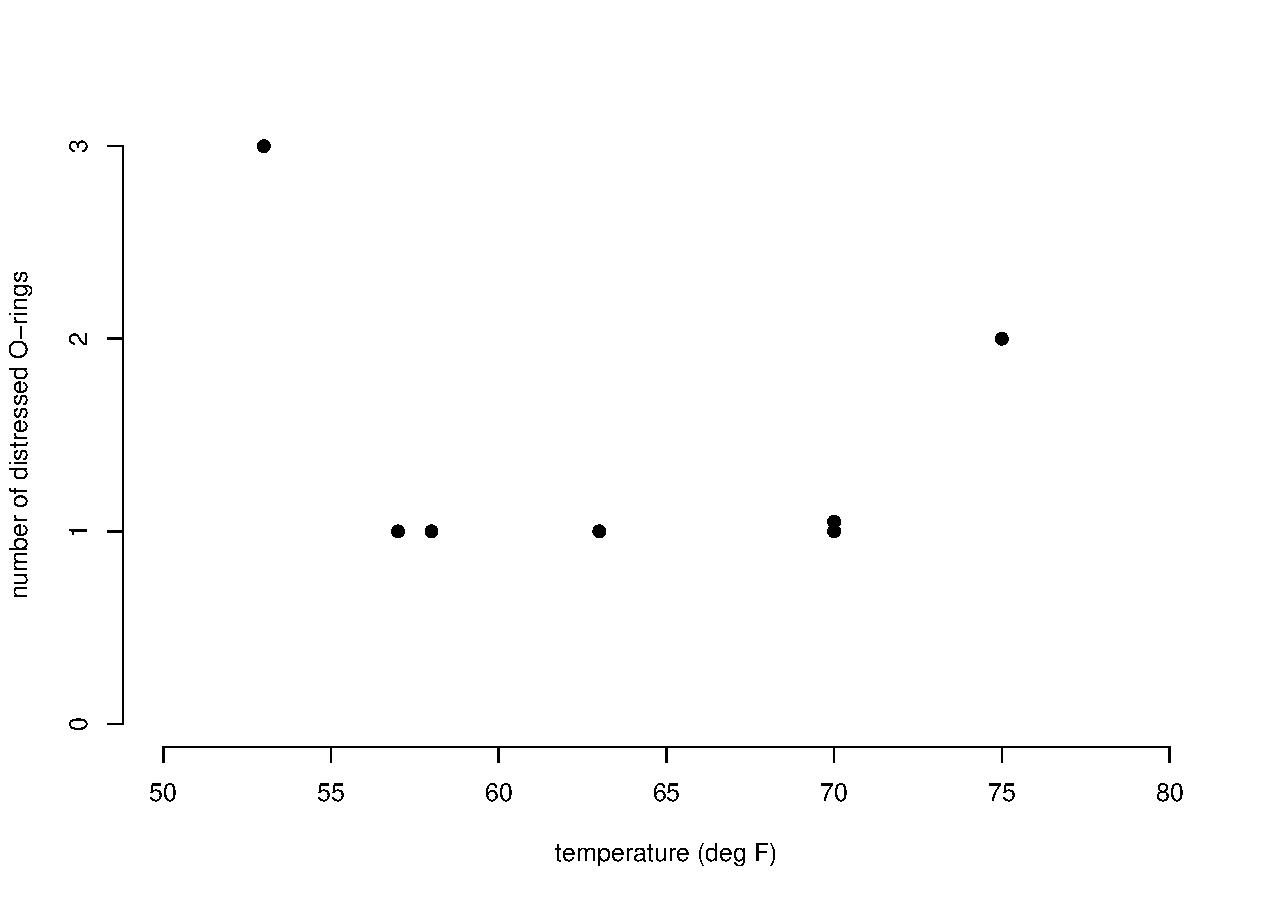
\includegraphics[width=0.75\linewidth]{images/shuttle1} 

}

\caption{Number of damaged O-rings plotted against temperature, for flights prior to 28/01/1986. Flights showing no incidents of distress have been omitted.  No clear association between the number of distressed O-rings and temperature is evident.}\label{fig:shuttle1}
\end{figure}

Flights giving zero incidents of thermal distress were not included in the graph. This was because it was felt that these flights did not contribute any information about the temperature effect. When the complete dataset (see Table \ref{tab:tabshuttle2} and Figure \ref{fig:shuttle2}) is examined it is clear that these flights \textbf{do} contribute extra information.

\begin{table}

\caption{\label{tab:tabshuttle2}Complete space shuttle data.  Number of damaged O-rings (out of a total of 6) for launches at a given temperature}
\centering
\begin{tabular}[t]{rllr}
\toprule
flight & date & damaged & temperature\\
\midrule
1 & 21/04/1981 & 0 & 66\\
2 & 12/11/1981 & 1 & 70\\
3 & 22/03/1982 & 0 & 69\\
4 & 11/11/1982 & 0 & 68\\
5 & 04/04/1983 & 0 & 67\\
\addlinespace
6 & 18/06/1983 & 0 & 72\\
7 & 30/08/1983 & 0 & 73\\
8 & 28/11/1983 & 0 & 70\\
9 & 03/02/1984 & 1 & 57\\
10 & 06/04/1984 & 1 & 63\\
\addlinespace
11 & 30/08/1984 & 1 & 70\\
12 & 05/10/1984 & 0 & 78\\
13 & 08/11/1984 & 0 & 67\\
14 & 24/01/1985 & 3 & 53\\
15 & 12/04/1985 & 0 & 67\\
\addlinespace
16 & 29/04/1985 & 0 & 75\\
17 & 17/06/1985 & 0 & 70\\
18 & 29/07/1985 & 0 & 81\\
19 & 27/08/1985 & 0 & 76\\
20 & 03/10/1985 & 0 & 79\\
\addlinespace
21 & 30/10/1985 & 2 & 75\\
22 & 26/11/1986 & 0 & 76\\
23 & 21/01/1986 & 1 & 58\\
24 & 28/01/1986 & ? & 31\\
\bottomrule
\end{tabular}
\end{table}

\begin{figure}

{\centering 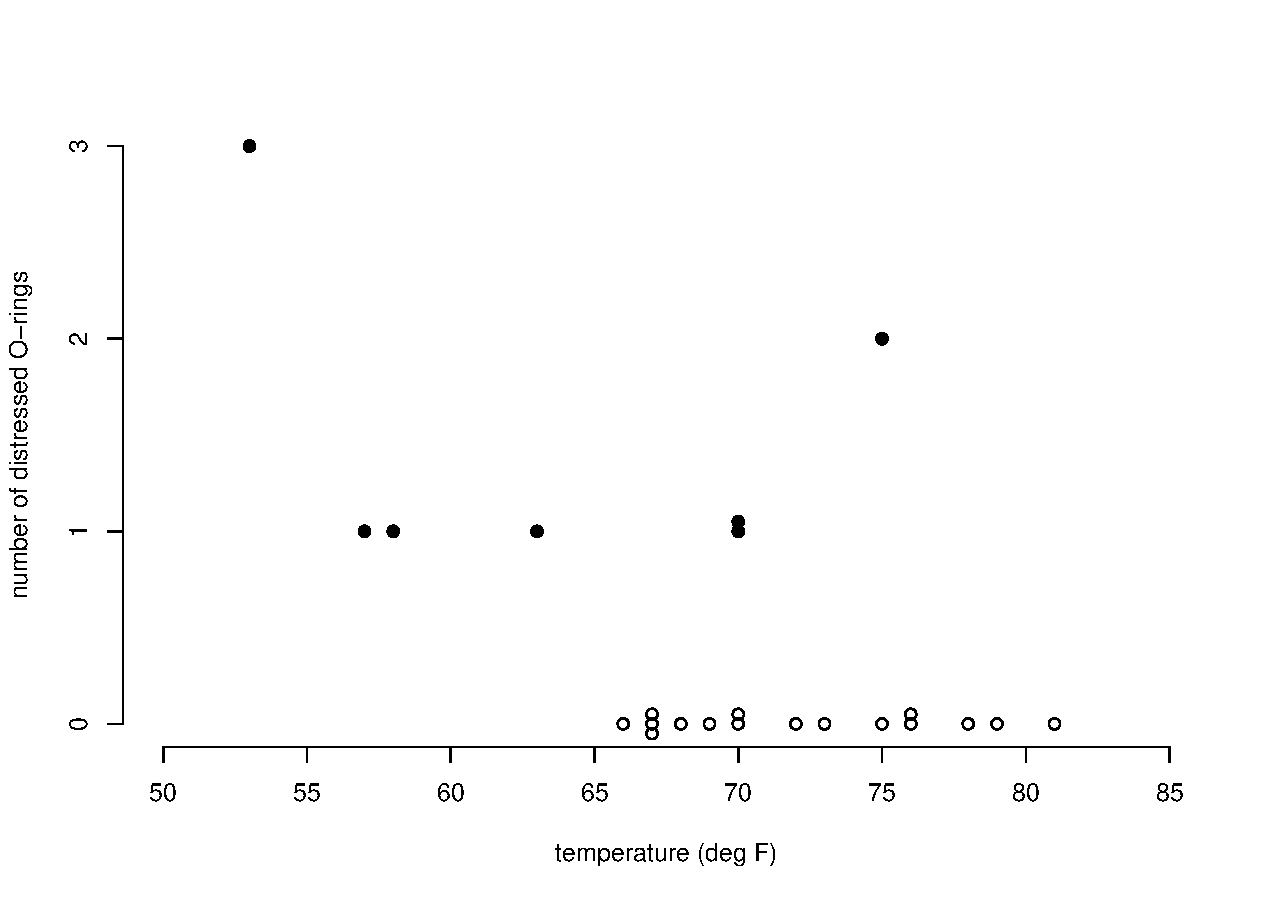
\includegraphics[width=0.75\linewidth]{images/shuttle2} 

}

\caption{Number of damaged O-rings plotted against temperature, for flights prior to 28/01/1986. Flights showing no incidents of distress have been included as hollow circles.  A clear negative association between the number of distress O-rings and temperature is evident.}\label{fig:shuttle2}
\end{figure}

The enquiry into the Challenger accident concluded that a more careful analysis of the O-ring data would have revealed the apparent effect of temperature on O-ring performance.

What can we learn from this example?

\begin{itemize}
\tightlist
\item
  Data analyses can have life and death consequences. Statisticians can be very important people!\\
\item
  Statistical analyses should use \textbf{all} the data. In this example only a non-random sample of the data are used. Removing some of the data had dire consequences. Values of zero are still data.
\item
  It is dangerous to extrapolate beyond the range of your data. No data were available below 50\(^\circ\)F. The forecast temperature of 31\(^\circ\)F was much lower than this.
\end{itemize}

After the accident \citet{shuttle} estimated the probability of a catastrophic O-ring failure (that is, one that would cause an explosion) at 31\(^\circ\)F to be at least 0.13, which is large considering that seven lives were at stake. {[}To quantify their \textbf{uncertainty} they estimate that the probability is 90\% certain to be between 0.03 and 0.37.{]} However, it should certainly be made clear that this estimate may not be at all reliable. For example, it could be that as temperature decreases below 50\(^\circ\)F the risk of an accident increases much more quickly than the statistical analysis suggests.

The plot in Figure \ref{fig:shuttle3} gives you an idea of one of the analyses that \citet{shuttle} carried out. The sample proportions
of O-rings showing thermal distress (number of O-rings showing distress divided by 6) are plotted against temperature. Also plotted is a smooth curve fitted to these data. {[}This analysis is beyond scope of STAT0002/0003. You may study this type of model in STAT0023.{]}

\begin{figure}

{\centering 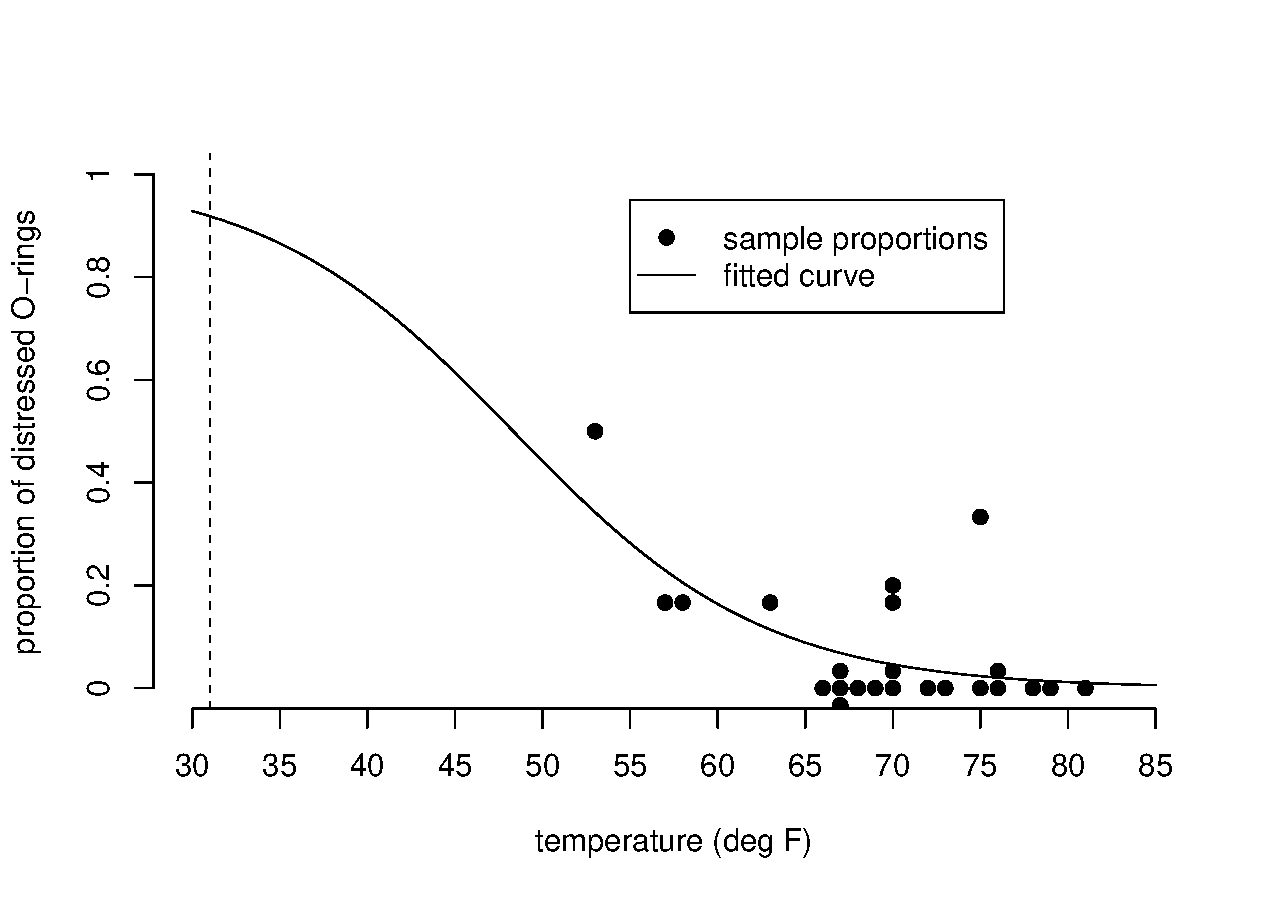
\includegraphics[width=0.75\linewidth]{images/shuttle3} 

}

\caption{Proportion of O-rings showing some thermal distress plotted against temperature, with fitted logistic curve.  The fitted curve reflects the apparent negative association between this proportion and temperature.}\label{fig:shuttle3}
\end{figure}

\hypertarget{uncertainty}{%
\subsection{Uncertainty}\label{uncertainty}}

Suppose there is a true curve, of the same general type as the one in Figure \ref{fig:shuttle3}, which describes how the probability that an O-ring is damaged depends on temperature. We use the NASA test flight data to guess, or \textbf{estimate} the exact shape of this true curve. The curve in figure \ref{fig:shuttle3} is \textbf{not} the true curve, it is an \textbf{estimate} of the true curve based on these data.

If NASA repeated their launches, at exactly the same temperatures, these new data on the number of damaged O-rings would not be the same as the old data and the shape of the new estimated curve would be different from the shape of the old estimated curve. It may be that these 2 curves are quite similar or it could be that they are very different. We could ask them, very politely, repeat this process many times to get a large number of different sets of data. Each set of data produces an estimated curve.

The dataset (and its estimated curve) we have is just one of many possible datasets that could be produced. We can imagine picking this dataset (and curve) at random from a big bag of possible datasets (and curves). These ideas are summarised in Figure \ref{fig:shuttlediagram}.

\begin{figure}

{\centering 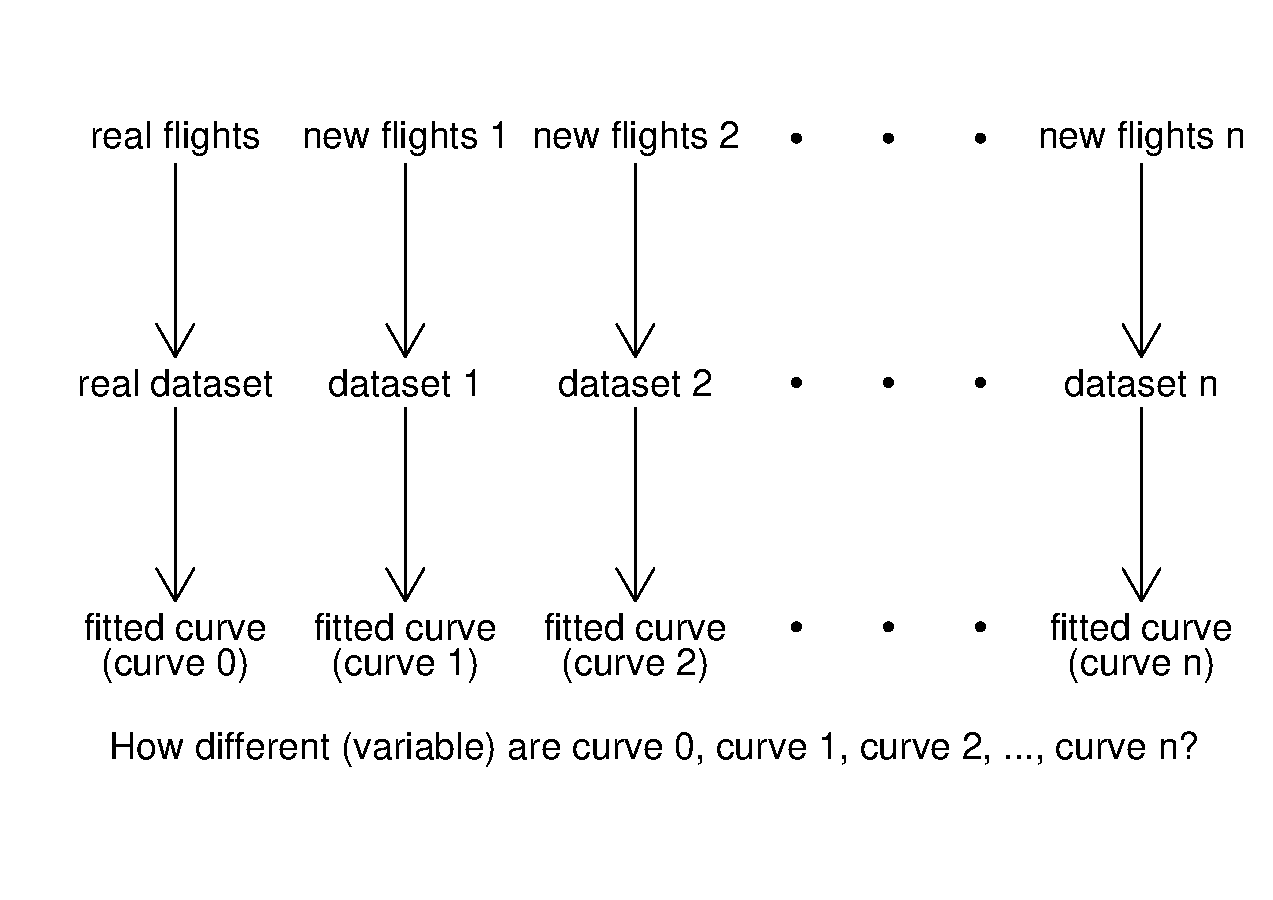
\includegraphics[width=0.75\linewidth]{images/shuttle_diagram} 

}

\caption{Diagram to illustrate the idea of repeating an experiment many times.  Each simulated set of flights leads to its own dataset and fitted logistic curve.}\label{fig:shuttlediagram}
\end{figure}

Suppose that the estimated curves from the possible datasets are very similar to each other. We say that their \textbf{variability} is small. If this is the case then it doesn't matter much which dataset we picked from the big bag of possible datasets: the results are similar for all datasets. Therefore, we can be fairly certain that the results we got from the dataset we have are close to the truth. Therefore the \textbf{uncertainty} surrounding the results is small.

On the other hand, if the estimated curves from the possible datasets are very different to each other then their \textbf{variability} is large. If this is the case then the results will be very different depending on which dataset we pick. Therefore, it is possible that the results we got from the dataset are very far from the truth. Therefore the \textbf{uncertainty} about the results is large.

We can see that \textbf{variability} and \textbf{uncertainty} are closely related. Small variability tends to produce small uncertainty, whereas large variability tends to produce large uncertainty. As we might expect the amount of data, (or, more precisely, the amount of \textbf{information} in the data) matters. Large datasets, with lots of information, tend to produce small variability in the results and therefore small uncertainty. Small datasets, with small amounts of information, tend to produce large variability in the results and therefore large uncertainty.

So, how can we quantify how much uncertainty there is in the space shuttle example? It is unlikely that NASA will carry out all their launches again just for us. However, it is possible for us to produce (\textbf{simulate}) on a computer our own, fake, datasets using the estimated curve in Figure \ref{fig:shuttle3}. If this curve (and the assumptions used to produce it) are correct, this is equivalent to NASA carrying out more test flights: the simulated datasets have exactly the same statistical properties as the real dataset. In summary, we

\begin{itemize}
\tightlist
\item
  create a large number of fake (\textbf{simulated}) datasets;
\item
  for each dataset we estimate a curve to describe how the probability of O-ring damage depends on temperature;
\item
  examine how much the curves, and the estimate of probability at different temperatures vary between the simulated datasets.
\end{itemize}

Figure \ref{fig:shuttlesimcurves} shows 50 simulated curves and the curve estimated from the real data.

\begin{figure}

{\centering 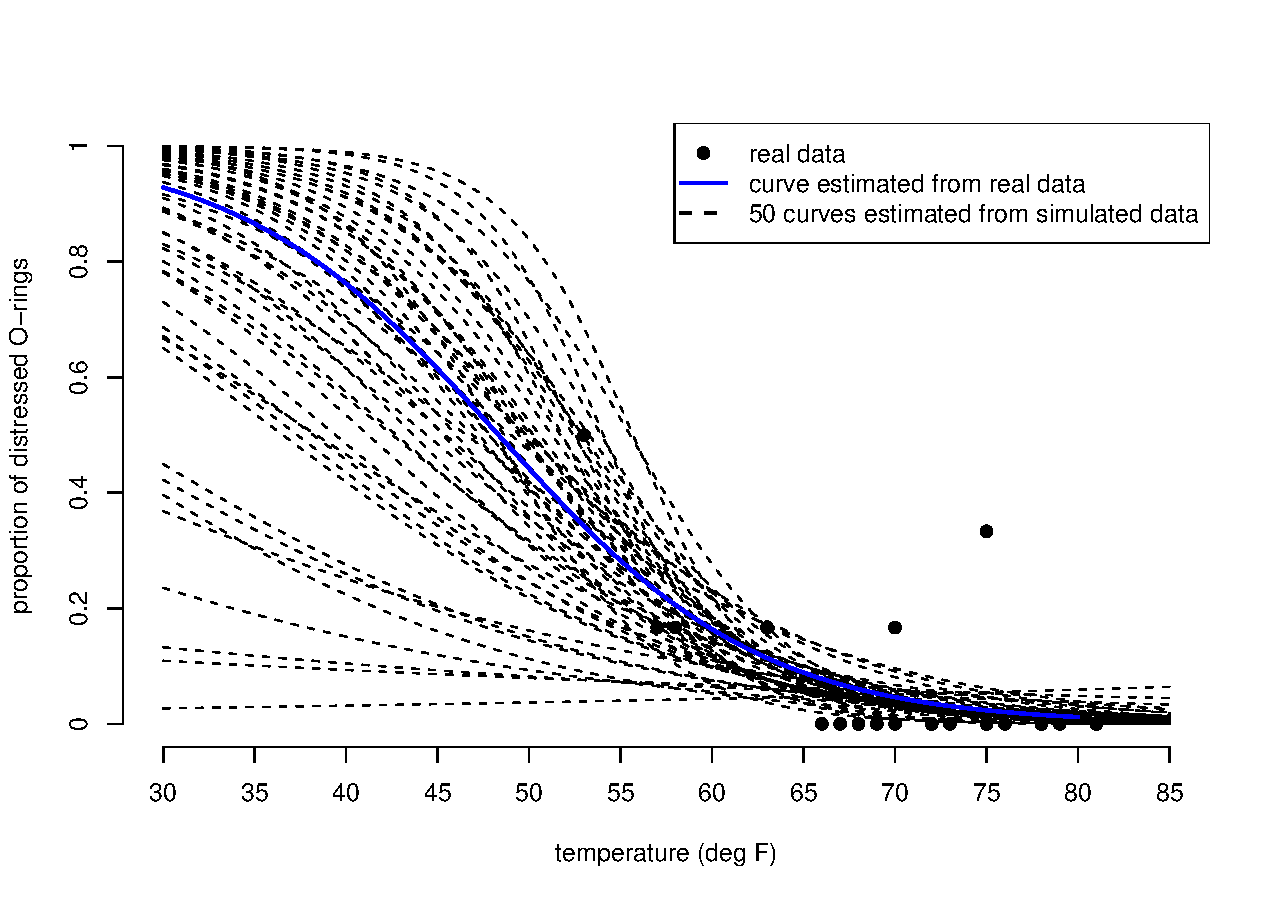
\includegraphics[width=0.75\linewidth]{images/shuttle_simcurves} 

}

\caption{50 curves fitted to simulated shuttle test flight data. The curves are similar over the range of temperatures observed in the data (53 to 81 degrees F), but vary greatly for lower temperatures, such as 31 degrees F.}\label{fig:shuttlesimcurves}
\end{figure}

There is a lot of variability in these curves. Notice that the curves are quite close to each other for high temperatures - where we have some data - but that they are very spread out for low temperatures - where we have no data. This is confirmed by figure \ref{fig:shuttlesim} which shows how the estimated probability of O-ring damage depends on temperature.

\begin{figure}

{\centering 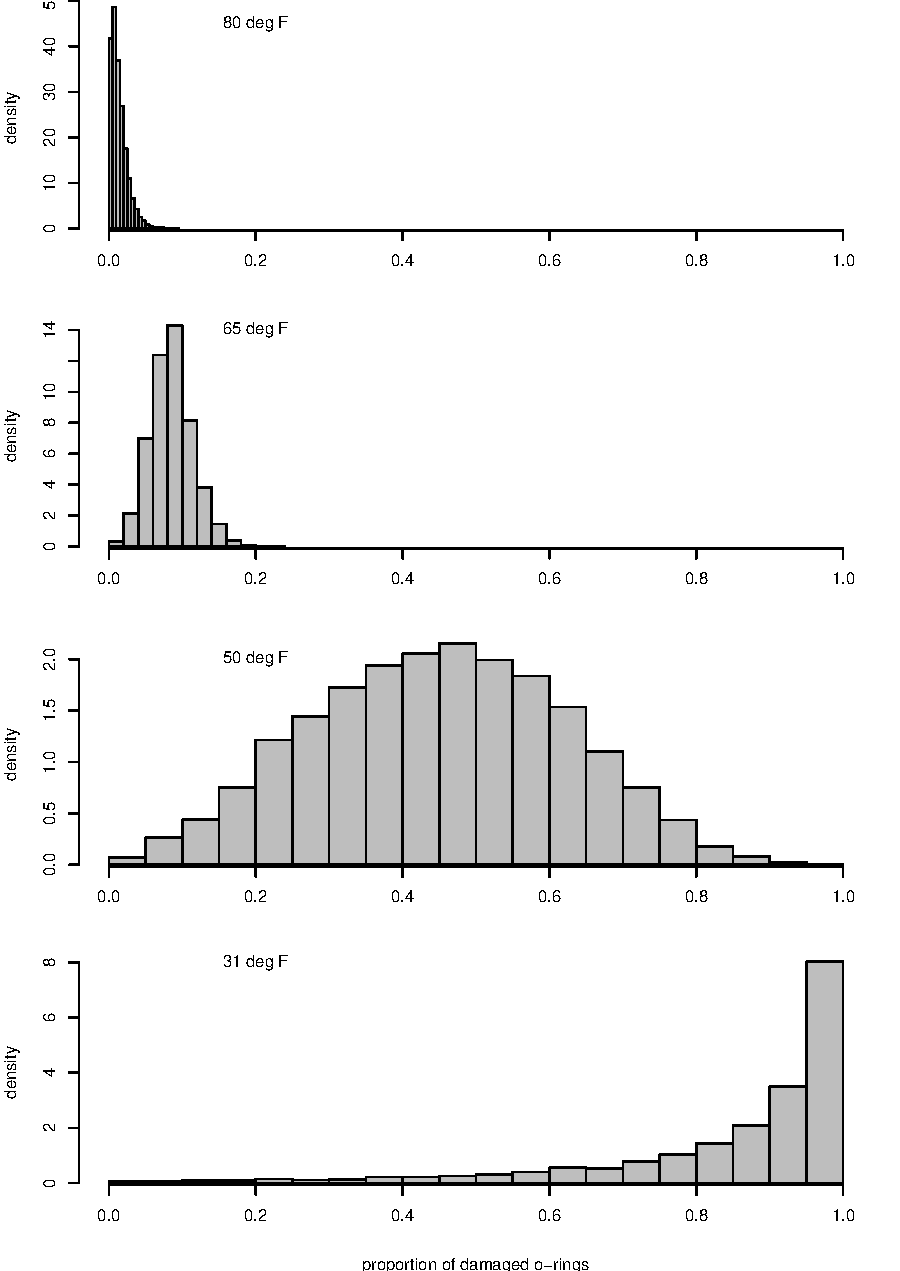
\includegraphics[width=0.75\linewidth]{images/shuttle_sim} 

}

\caption{Histograms of estimated probabilities of O-ring damage at different temperatures.}\label{fig:shuttlesim}
\end{figure}

There is a large amount of uncertainty about the esimatated probabilities, particularly at 31\(^\circ\)F, where it really mattered.

To show the effect of sample size (the size of the dataset) we simulate datasets which are larger than the real dataset and see how much the curves fitted to these data vary between the datasets. Figure \ref{fig:shuttlesimcurves10} shows the estimated curves from 50 datasets, each of which is 10 times the size of the real dataset. Figure \ref{fig:shuttlesimcurves100} shows curves for datasets which are 100 times the size of the original dataset. As the sample size increases the variability decreases and so the uncertainty decreases.

\begin{figure}

{\centering 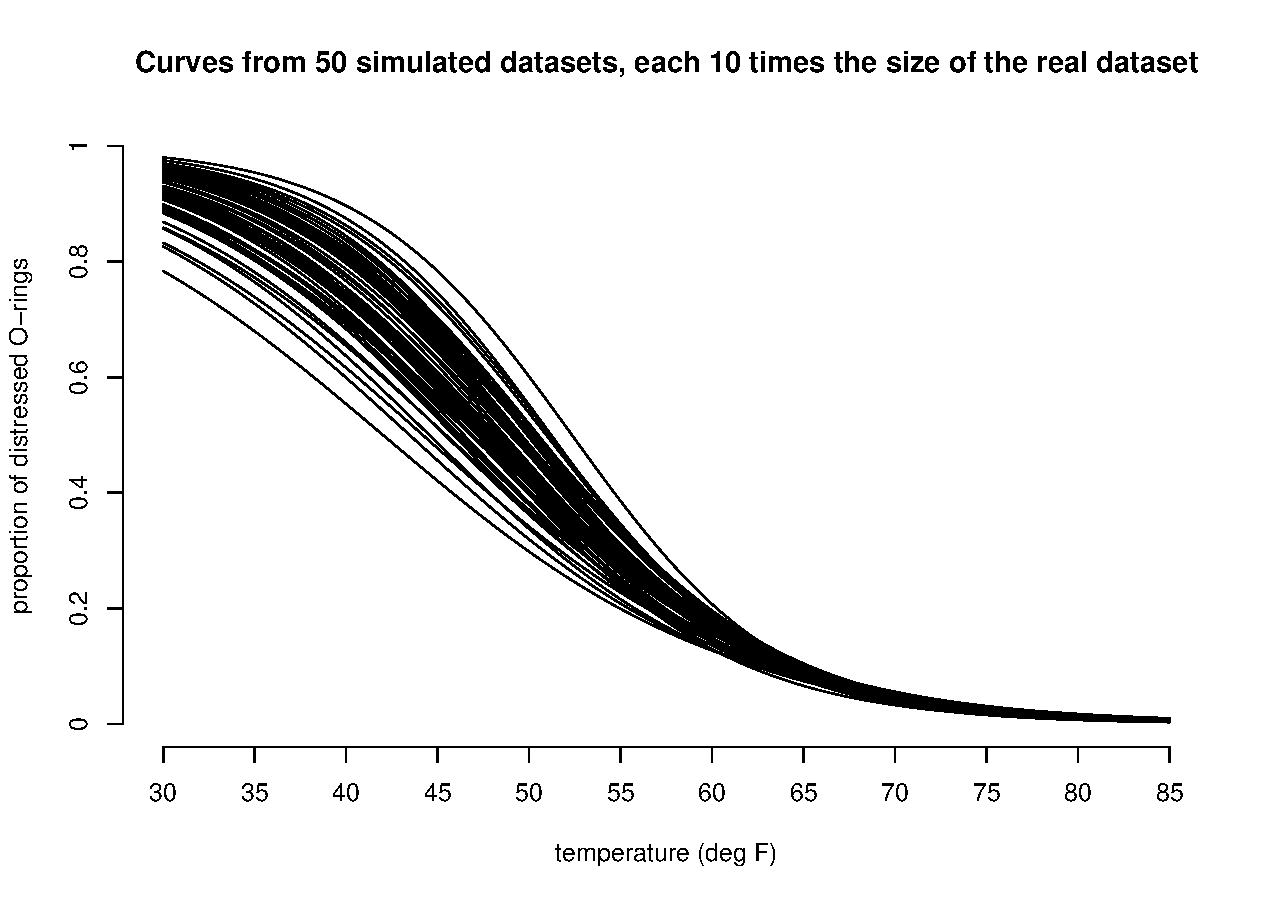
\includegraphics[width=0.75\linewidth]{images/shuttle_simcurves10} 

}

\caption{50 curves fitted to simulated shuttle test flight datasets that are each 10 times the size of the real dataset.  In comparision to the curves based on the real dataset these curves vary less, but are still most variable for low temperatures.}\label{fig:shuttlesimcurves10}
\end{figure}

\begin{figure}

{\centering 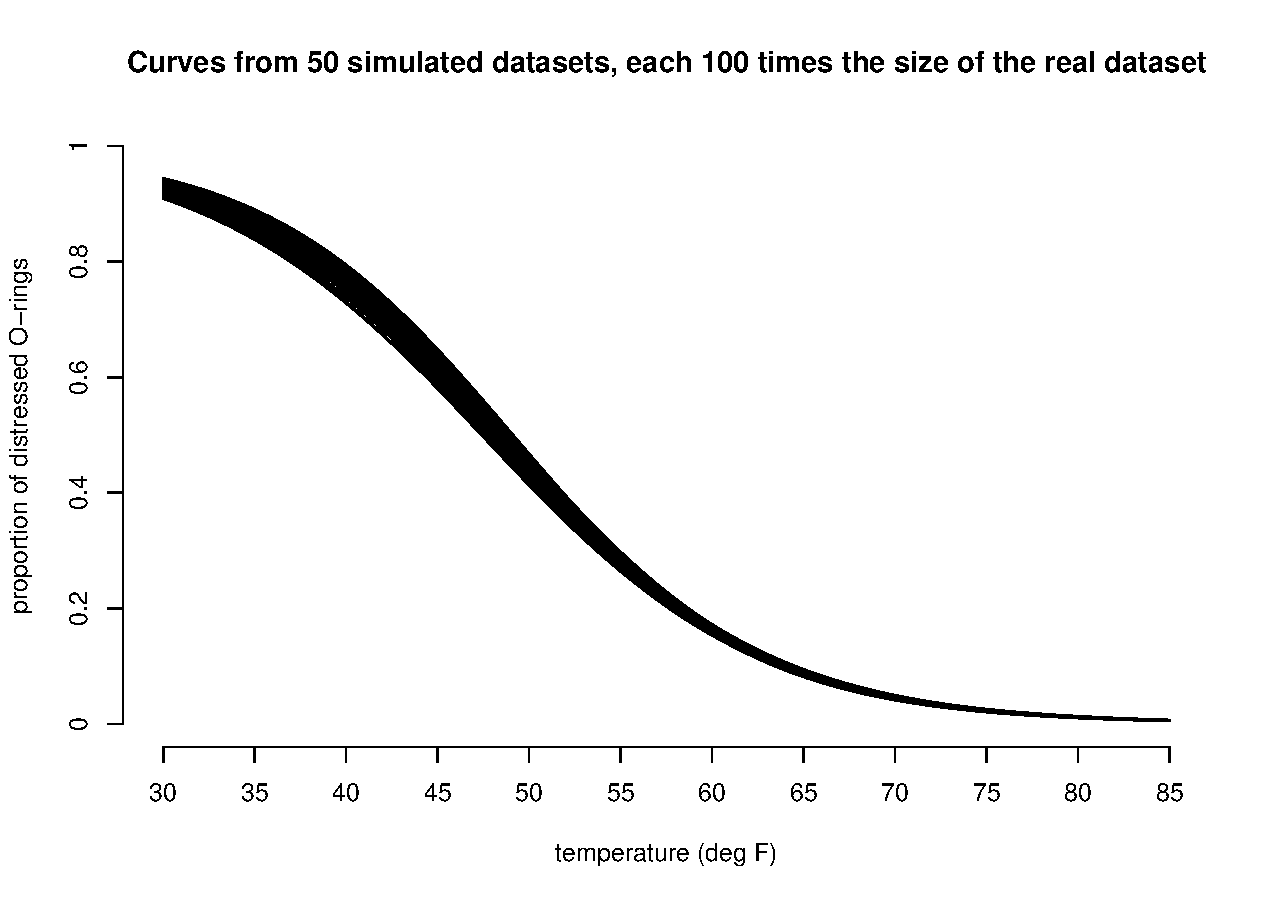
\includegraphics[width=0.75\linewidth]{images/shuttle_simcurves100} 

}

\caption{50 curves fitted to simulated shuttle test flight datasets that are each 100 times the size of the real dataset. In comparision to the curves based on the real dataset these curves vary much less, but are still most variable for low temperatures.}\label{fig:shuttlesimcurves100}
\end{figure}

\hypertarget{a-very-brief-introduction-to-stochastic-simulation}{%
\section{A very brief introduction to stochastic simulation}\label{a-very-brief-introduction-to-stochastic-simulation}}

This section contains words that we will not define until later in the course. Further information about stochastic simulation is available from the Stochastic Simulation section of the STAT0002 Moodle page.

In Statistics it is common to assess a statistical method based on how well it would perform if used repeatedly on a large number of new datasets, where we imagine that the new datasets have exactly the same statistical properties as the real data. In some cases it is possible to do this using mathematics. Alternatively, we can use a computer to produce some fake (simulated) datasets from a model that has been fitted to the real data. How can we do this?

Stochastic (stochastic simply means ``involving randomness'') simulation is based on the ability to generate a random number \(u\) between 0 and 1. Stochastic simply means ``involving randomness''. Your pocket calculator probably has a button to do this, perhaps called RAN\#. It is possible to transform this number \(u\) so that it looks like it has been drawn from the distribution required, e.g.~a binomial distribution or a normal distribution. If we produce a sequence \(u_1, u_2, \ldots, u_n\) of random numbers between 0 and 1 and transform them appropriately, then the transformed values will look like a random sample from the distribution required. Of course, because these values are produced by rule implemented by a computer they are not really random. However, if the rule is designed carefully, these values are close enough to being a random sample for our purposes.

For the purposes of the space shuttle experiment we simply need to simulate a 1 (O-ring distressed) with probability \(p\), and a 0 (0-ring not distressed) with probability \(1-p\). This is easy. If \(U\) is a random number between 0 and 1 then the probability that \(U < p\) is \(p\). Therefore, we define

\begin{equation}
X = 
\begin{cases} 
1 & \text{if } U < p, \\
0 & \text{if } U \geq p.
\end{cases}
\label{eq:xbin}
\end{equation}

For \(p=1/2\) this is like using a computer to flip an unbiased coin.

To simulate a fake space shuttle dataset we do the following for each of the 23 flights:

\begin{enumerate}
\def\labelenumi{\arabic{enumi}.}
\tightlist
\item
  set \(p\) to be the value of the fitted curve in Figure \ref{fig:shuttle3} corresponding to the flight temperature;
\item
  generate 6 random numbers \(u_1, \ldots, u_6\) between 0 and 1;
\item
  calculate \(x_1, \ldots, x_6\) using equation \eqref{eq:xbin};
\item
  calculate \(y=x_1+\cdots+x_6\), the total number of distressed O-rings.
\end{enumerate}

We have assumed that the 6 O-rings have the same probability of becoming distressed and are distressed independently of each other. In Chapter \ref{rvs} we will see that \(y\) is a value simulated from a binomial(6, \(p\)) distribution. We will use simulation several times in STAT0002 to study properties of statistical methods. All you need to know is that we can use a computer to produce fake data that look like they come from a certain probability distribution.

\hypertarget{descriptive}{%
\chapter{Descriptive statistics}\label{descriptive}}

The first important step in any data analysis is to \textbf{describe} the
available data. This is often called an \textbf{exploratory} or \textbf{initial} data analysis. It is normally not possible to just look at the dataset, especially if it is large, and just see any interesting structures. The task of a statistician is therefore to \textbf{extract} and \textbf{condense} the relevant information -- what is relevant will depend on the aim of the analysis. Some of the standard methods to do so are addressed in the next sections. Despite all the technicalities, always remember that the numbers / figures / plots produced for data must be \textbf{interpreted with regard to the problem or question at hand}, that is, always ask yourself ``what does this number / plot mean?''.

Before embarking on a formal statistical analysis of the data we should look at summaries of the data such as graphs, tables and summary statistics. This can be important to

\begin{enumerate}
\def\labelenumi{\arabic{enumi}.}
\tightlist
\item
  reveal problems with, or errors in, the data;
\item
  get a `feel' for the data;
\item
  identify interesting features of the data, e.g.~is treatment A very
  obviously better at treating a disease than treatment B?;
\item
  suggest how the data should be analysed;
\item
  present conclusions.
\end{enumerate}

In some cases the data summaries make it very clear what is going on and may
make more formal methods of statistical analysis unnecessary.

\hypertarget{types-of-data}{%
\section{Types of data}\label{types-of-data}}

Before analysing data it is important to consider what \textbf{type} they are. This will affect which statistics it is sensible to calculate, which graphs it is sensible to plot and which of the simple distributions we will study in Chapter \ref{simple} might be used for these data.

\hypertarget{qualitative-or-categorical-data}{%
\subsection{Qualitative or categorical data}\label{qualitative-or-categorical-data}}

Items are assigned to \textbf{groups} or \textbf{categories} based on some \textbf{qualitative} property. Examples:

\begin{itemize}
\tightlist
\item
  Hair colour: blonde, brown, red, black etc.
\item
  Smoking status: smoker, non-smoker;
\item
  Severity of illness: none, mild, moderate, severe;
\item
  Degree class: 3, 2ii, 2i, 1.
\end{itemize}

The data are \textbf{labels}: if numbers are assigned to the categories (e.g.~
0=smoker, 1=non-smoker) the numbers chosen do not mean anything in themselves.

Categorial data can be classified as either

\begin{itemize}
\tightlist
\item
  \textbf{nominal}: the categories are unordered, e.g.~hair colour, smoking status;
\item
  \textbf{ordinal}: the categories are ordered, e.g.~severity of illness, degree class.
\end{itemize}

An important special case is \textbf{binary} data: categorical data with only 2 categories. These data can be nominal (e.g.~male, female) or ordinal (e.g.~small, large).

Nominal data: describe by (relative) frequencies. It is sensible to quote the mode, but not the mean or median.

Ordinal data: It is sensible to quote the mode or median, but not the mean.

\hypertarget{quantitative-or-numerical-data}{%
\subsection{Quantitative or numerical data}\label{quantitative-or-numerical-data}}

Items are measured in some way based on some \textbf{quantitative} property. This produces a one, or more, \textbf{numbers}. Examples:

\begin{itemize}
\tightlist
\item
  Time, in hours;
\item
  Height, in cm;
\item
  Age, in years;
\item
  Number of damaged O-rings (see space shuttle investigation);
\item
  Number of births on one day at a particular hospital;
\item
  Number of units passed in first year.
\end{itemize}

Numerical data can be classified as either

\begin{itemize}
\tightlist
\item
  \textbf{Discrete}. Only certain values are possible (there are gaps between the possible values), e.g.~number of damaged O-rings, number of births, number of units passed in first year (0, 0.5, 1, 1.5, 2, 2.5, 3, 3.5, 4);
\item
  \textbf{Continuous}. In theory, \textbf{any} value within an interval of the real line
  is possible, e.g.~time, height, age.
\end{itemize}

Often discrete data are \textbf{counts}. Continuous data usually come from measurement. In practice continuous data are recorded discretely, e.g.~to two decimal places.

\hypertarget{interval-data-and-ratio-data}{%
\subsubsection*{Interval data and ratio data}\label{interval-data-and-ratio-data}}
\addcontentsline{toc}{subsubsection}{Interval data and ratio data}

Quantitative data can be further classified as \textbf{interval} or \textbf{ratio}. Both interval data and ratio data have the property that an increase of 1 unit means the same whether it is from, say, 1 to 2 or from 10 to 11. However,

\begin{itemize}
\tightlist
\item
  a ratio scale has a natural zero, for example, temperature measured in degrees Kelvin;
\item
  an interval scale does not have a natural zero, for example temperature
  measured in Fahrenheit.
\end{itemize}

Ratios are only meaningful on a ratio scale. For example,

\begin{itemize}
\tightlist
\item
  IQ: A zero IQ does not exist. A person with an IQ of 120 is not twice as intelligent as a person with an IQ of 60. Therefore, IQs are interval data.
\item
  Income: A zero income does exist. A person whose take-home income is \pounds 20,000 does earn twice as much as some whose take-home income is \pounds 10,000.Therefore, incomes are ratio data.
\end{itemize}

\hypertarget{describing-distributions}{%
\section{Describing distributions}\label{describing-distributions}}

In describing the distribution of one variable the following it is important to
examine the following.

\begin{enumerate}
\def\labelenumi{\arabic{enumi}.}
\tightlist
\item
  \textbf{Location / average / central tendency of the data}. Where is the centre of the distribution? What is a typical value?\\
\item
  \textbf{Spread / variability / dispersion / scale}. How \textbf{variable} are the data? How far are they spread out?
\item
  \textbf{Shape}. What shape is the distribution of the data? In particular, is it \textbf{symmetric} or \textbf{skewed}, and if skewed, which way? A long tail to the right is called \textbf{positive skew} (or right skew or skewed to the right). A long tail to the left is known as a \textbf{negative skew} (or left skew or skewed to the left). Positive skew is much more common than negative skew. Figure \ref{fig:shapes} gives some examples of shapes of symmetric, positive skew and negative skew distributions. In addition to being symmetric the plot in the top left of Figure \ref{fig:shapes} of figure is bell-shaped. This shape is the shape of a \textbf{normal distribution} (see Section \ref{normal}). The normal distribution is an important distribution in Statistics. We may wish to decide whether the data look like they have come from a normal distribution.
\item
  \textbf{Outliers}. Are there any outliers, that is, observations that appear to be out of line with the pattern of the rest of the data? This issue can also be hard to judge. For example, with a small number of observations, it is difficult to distinguish between data from a heavily skewed distribution and data from a symmetric distribution with outliers. What constitutes an outlier depends on the context so there is no rigid rule for defining/detecting outliers. The intended statistical analysis also matters. We will consider how to deal with outliers (in the context of linear regression) in Section \ref{outliers}.
\item
  \textbf{Is there anything else to report?} Note any \textbf{unusual features}
  about the data. Are there particular numbers which appear more often than we could expect? Do the data separate into groups?
\end{enumerate}

\begin{figure}

{\centering 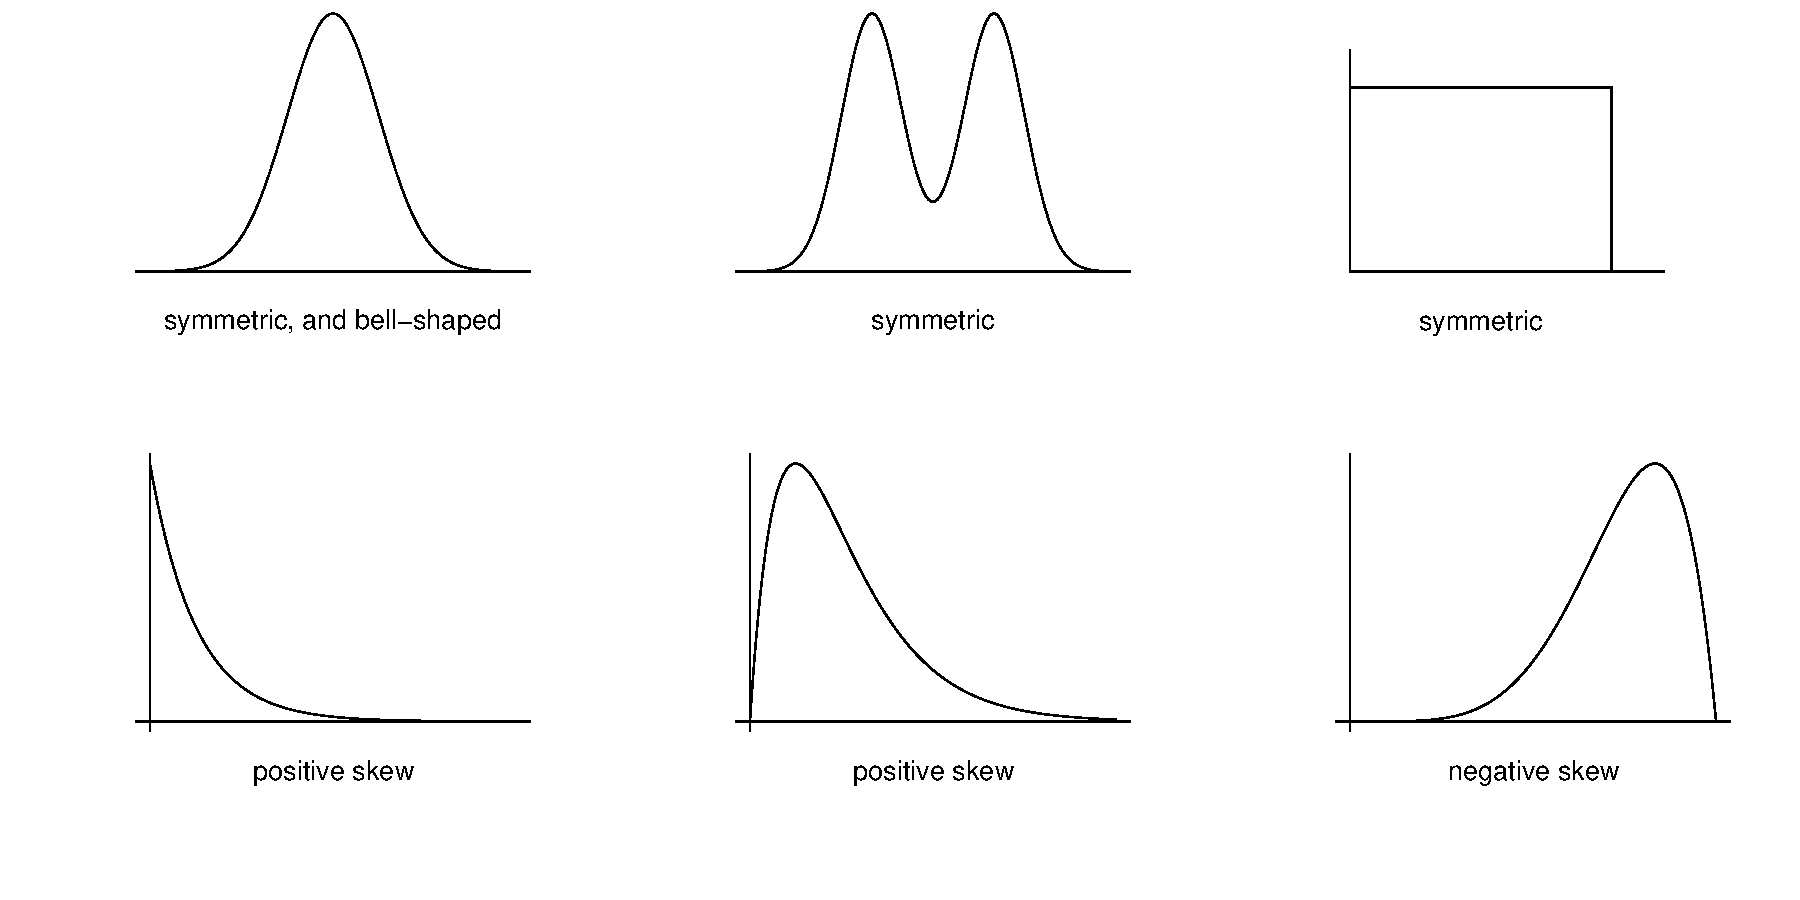
\includegraphics[width=0.75\linewidth]{images/shapes} 

}

\caption{Examples of shapes of symmetric, positively skewed and negatively skewed distributions.}\label{fig:shapes}
\end{figure}

We will look at 3 ways basic tools which are used to describe and summarise data: summary statistics, tables and graphs. We can use a combination of these. For example summary statistics may be presented in a table or a graph. Carefully produced graphs are often the best way to describe, explore and summarise a set of data. Summary statistics reduce the data to a small set of numbers. Tables can retain more information but do not work well for datasets which are large or have many variables. In contrast graphs can show most, if not all, the information in the data and reveal complex relationships.

\hypertarget{example-oxford-births-data}{%
\subsection*{Example: Oxford births data}\label{example-oxford-births-data}}
\addcontentsline{toc}{subsection}{Example: Oxford births data}

Table \ref{tab:taboxbirths} shows the times (in hours) spent by 95 women giving birth in the delivery suite of the John Radcliffe Hospital in Oxford during 1 week. These are ratio data. At first we ignore the fact that the data are recorded on different days.

\begin{table}

\caption{\label{tab:taboxbirths}Time (in hours) spent by each of 95 women giving birth at the John 
Radcliffe hospital in Oxford, UK, during a particular week.}
\centering
\begin{tabular}[t]{rrrrrrr}
\toprule
day1 & day2 & day3 & day4 & day5 & day6 & day7\\
\midrule
2.10 & 4.00 & 2.60 & 1.50 & 2.50 & 4.00 & 2.00\\
3.40 & 4.10 & 3.60 & 4.70 & 2.50 & 4.00 & 2.70\\
4.25 & 5.00 & 3.60 & 4.70 & 3.40 & 5.25 & 2.75\\
5.60 & 5.50 & 6.40 & 7.20 & 4.20 & 6.10 & 3.40\\
6.40 & 5.70 & 6.80 & 7.25 & 5.90 & 6.50 & 4.20\\
\addlinespace
7.30 & 6.50 & 7.50 & 8.10 & 6.25 & 6.90 & 4.30\\
8.50 & 7.25 & 7.50 & 8.50 & 7.30 & 7.00 & 4.90\\
8.75 & 7.30 & 8.25 & 9.20 & 7.50 & 8.45 & 6.25\\
8.90 & 7.50 & 8.50 & 9.50 & 7.80 & 9.25 & 7.00\\
9.50 & 8.20 & 10.40 & 10.70 & 8.30 & 10.10 & 9.00\\
\addlinespace
9.75 & 8.50 & 10.75 & 11.50 & 8.30 & 10.20 & 9.25\\
10.00 & 9.75 & 14.25 &  & 10.25 & 12.75 & 10.70\\
10.40 & 11.00 & 14.50 &  & 12.90 & 14.60 & \\
10.40 & 11.20 &  &  & 14.30 &  & \\
16.00 & 15.00 &  &  &  &  & \\
\addlinespace
19.00 & 16.50 &  &  &  &  & \\
\bottomrule
\end{tabular}
\end{table}

\hypertarget{summary-statistics}{%
\section{Summary statistics}\label{summary-statistics}}

One way to summarise a dataset is to calculate numerical summaries called \textbf{summary statistics}. Summary statistics can be used as indicators of the location, spread and shape of the data (although looking at a plot can be more helpful).

\hypertarget{fivenumber}{%
\subsection{Five number summary}\label{fivenumber}}

A useful first impression of the distribution of quantitative or ordinal data is given by the a five number summary. As we will see later, the five number summary involves quantities called \textbf{sample quantiles}. These are estimates of theoretical quantities that we will study in Chapter \ref{rvs}. There is more than one way to calculate sample quantiles. For example, the R statistical package has 9 options in its \texttt{quantile()} function. The particular method given below is just one of these options.

If a dataset of observations, \(x_1,x_2,\ldots,x_n\), is arranged in order of size as \[ x_{(1)} \leq x_{(2)} \leq \cdots \leq x_{(n)}\] then the \textbf{sample median} is the `middle' value (halfway between \(x_{(1)}\) and \(x_{(n)}\)), that is,
\[ m=x_{(\frac{1}{2}(n+1))}\,.\]
The median is a measure of location.

Informally, we can think of the \textbf{sample lower quartile} as the sample median of the lower half of the data, or, equivalently, as the value that divides the lower 25\% of the data from the rest of the data. One way to estimate this is
\[ q_L=x_{(\frac{1}{4}(n+1))} \,.\]
Similarly, we can think of the \textbf{sample upper quartile} as the sample median of the upper half of the data, which we could estimate using
\[ q_U=x_{(\frac{3}{4}(n+1))}\,.\]
If \(m, q_L\) or \(q_U\) do not correspond directly with one of the observations
then we can use linear interpolation. Suppose that \(n=44\). Then we could calculate the sample median using
\[x_{(22.5)}=x_{(22)}+\frac12\left(x_{(23)}-
x_{(22)}\right)=\frac{x_{(22)}+x_{(23)}}{2}, \]
the sample lower quartile using
\[ x_{(11.25)}=x_{(11)}+\frac14\left(x_{(12)}-
x_{(11)}\right)=\frac34\,x_{(11)}+\frac14\,x_{(12)}, \]
and the sample upper quartile using
\[x_{(33.75)}=x_{(33)}+\frac34\left(x_{(34)}-
x_{(33)}\right)=\frac14\,x_{(33)}+\frac34\,x_{(34)}.\]
This is not the only possibility: you may find that different methods are used in some textbooks and by some computer packages. If the data are ordinal then interpolating may not make sense.

The quartiles \(q_L, m, q_U\) (so called because they divide the data into 4 equal parts) are sometimes denoted \(q_1, q_2\) and \(q_3\).

The \textbf{five number summary} of the data set is the set of values
\[(x_{(1)},q_L,m,q_U,x_{(n)})\,\]
that is, the sample minimum, lower quartile, median, upper quartile and maximum.

The \textbf{range} is defined as \(x_{(n)}-x_{(1)}\) and the \textbf{inter-quartile
range} (IQR) as \(q_U-q_L\). The range and IQR are measures of spread.

More generally, we could could calculate sample \textbf{quantiles}, or \textbf{percentiles}. The 30\% quantile, for example, is the value at or below which 30\% of the data lie. The 100\(p\)\% sample quantile is \(x_{(p(n+1))}\). When \(p(n+1)\) is not an integer, \(x_{(p(n+1))}\) can be calculated using linear interpolation. Note: the number of quantiles which we can estimate reliably depends on the \textbf{sample size} \(n\). For example, if \(n=3\), it doesn't make sense to try to estimate the 10\% quantile. In this case \(q_L=x_{(1)}, m=x_{(2)}\) and \(q_U=x_{(3)}\).

Sometimes the sample size \(n\) is added to the five number summary. The
sample size can be of interest in its own right, for example when it records the
number of times an event of interest occurs in a fixed period of time,
for example, the number of births in the delivery suite of the John Radcliffe
hospital in Oxford during one week.

\hypertarget{meanstdev}{%
\subsection{Mean and standard deviation}\label{meanstdev}}

The most well known descriptive measures of \textbf{numerical} data are the (arithmetic) mean and the standard deviation.

The \textbf{sample mean}, a measure of location, is defined as the arithmetic average
\[ \bar{x}\,=\,\frac{1}{n}(x_1+x_2+\cdots+x_n)=\frac{1}{n}\sum_{i=1}^n x_i\,.\]
The \textbf{sample variance}, a measure of spread, is
\[ s^2 \,\,=\,\, \frac{1}{n-1}\sum_{i=1}^n (x_i-\bar{x})^2 \,\,=\,\, \frac{1}{n-1}\left\{\sum_{i=1}^n x_i^2 - n(\bar{x})^2\right\}\,.\]
The \textbf{sample standard deviation}, also a measure of spread, but has the same units as the data, is
\[ s=\sqrt{s^2} \,.\]
For example, if the units of the data are metres then the units of the variance are metres\(^2\) and the units of the standard deviation are metres.

The formula (with a different denominator)
\[ \frac{1}{n}\sum_{i=1}^n (x_i-\bar{x})^2 \,,\]
which is used by some calculators is equal to \(s^2 (1-1/n)\), \textbf{not} \(s^2\). For large \(n\) the values of \(s^2\) and \(s^2(1-1/n)\) will be close.

For data that are very skewed, or contain outliers, the sample median may be a more appropriate measure of location than the sample mean. This is because the value of the sample mean is strongly influenced by large or small values. For example, if the data are positively skewed the value of the mean may be much larger than where we would judge by eye the centre of the data to be. However, for data which are fairly symmetric there are reasons to prefer the sample mean to the sample median. For example,

\begin{itemize}
\tightlist
\item
  the sample mean is easier to calculate;
\item
  if samples are taken repeatedly the sample mean varies less than the sample median.
\end{itemize}

We will examine this in more detail in Section \ref{good}. Similarly, for a measure of spread, the sample standard deviation may be preferred for approximately symmetric data with no outliers, otherwise the IQR is preferable.

\hypertarget{mode}{%
\subsection{Mode}\label{mode}}

For categorical data or discrete data the mode is the value (or values) which occurs most often. The concept of a mode is relevant to continuous data, but it is less obvious how we might estimate this using data. We return to this in Section \ref{locations}. The mode is a measure of location.

\hypertarget{examples}{%
\subsubsection*{Examples}\label{examples}}
\addcontentsline{toc}{subsubsection}{Examples}

What are the sample mean, median and mode of the following data?

\begin{quote}
blonde hair, red hair, red hair, black hair
\end{quote}

What are the sample mean, median and mode of the degree classes?

\begin{quote}
3, 2ii, 2i, 1, 1
\end{quote}

What are the sample mean, median and mode of the following numbers?

\begin{quote}
10, 350
\end{quote}

Which measures of location are sensible for different types of data? Consider each case in Table \ref{tab:whichmeasures}.

\begin{longtable}[]{@{}lccc@{}}
\caption{\label{tab:whichmeasures} Types of data and measures of location.}\tabularnewline
\toprule()
& mean & median & mode \\
\midrule()
\endfirsthead
\toprule()
& mean & median & mode \\
\midrule()
\endhead
nominal & & & \\
ordinal & & & \\
numerical & & & \\
\bottomrule()
\end{longtable}

\hypertarget{symmetry}{%
\subsection{Symmetry}\label{symmetry}}

Many standard statistical methods work best when the data are distributed symmetrically. Looking at a graph is the best way to examine whether this is true. Some books/websites suggest comparing the values of the sample mean and sample median as a way to judge whether the data are approximately symmetric, as summarised in Table \ref{tab:thumb}. However, we will see that this rule-of-thumb can be \textbf{very misleading}.

\begin{longtable}[]{@{}cccc@{}}
\caption{\label{tab:thumb} Relative values of the sample mean and median and what this \textbf{might} suggest in some cases.}\tabularnewline
\toprule()
mean \(<\) median & mean = median & mean \(>\) median & \\
\midrule()
\endfirsthead
\toprule()
mean \(<\) median & mean = median & mean \(>\) median & \\
\midrule()
\endhead
negative skew & symmetric & positive skew & \\
\bottomrule()
\end{longtable}

\hypertarget{example.-oxford-births-data}{%
\subsubsection*{Example. Oxford births data}\label{example.-oxford-births-data}}
\addcontentsline{toc}{subsubsection}{Example. Oxford births data}

Table \ref{tab:oxfivenum} gives the five-number summary of the Oxford birth times data.

\begin{longtable}[]{@{}ccccc@{}}
\caption{\label{tab:oxfivenum} Sample five-number summary of the Oxford birth times data.}\tabularnewline
\toprule()
\(x_{(1)}\) & \(q_L\) & \(m\) & \(q_U\) & \(x_{(n)}\) \\
\midrule()
\endfirsthead
\toprule()
\(x_{(1)}\) & \(q_L\) & \(m\) & \(q_U\) & \(x_{(n)}\) \\
\midrule()
\endhead
1.50 & 4.90 & 7.50 & 9.75 & 19.00 \\
\bottomrule()
\end{longtable}

Half of the women took between approximately 5 and 10 hours to give birth.The quickest delivery was 90 minutes and the longest 19 hours. The mean \(\bar{x}\) is 7.72 hours and the standard deviation is 3.57 hours. The fact that sample mean \(>\) sample median suggest that the data are slightly positively skewed, but this is something that we should confirm by looking at a suitable graph (see Section \ref{graphs}).

\hypertarget{measures-of-skewness}{%
\subsubsection*{Measures of skewness}\label{measures-of-skewness}}
\addcontentsline{toc}{subsubsection}{Measures of skewness}

Usually the best way to examine the shape of a distribution is to look at a graph see section \ref{graphs}. In addition we could calculate summary measures of skewness, such as: the \textbf{standardized sample skewness}
\[\mbox{skewness} = \frac{\displaystyle\frac1n \sum_{i=1}^n (x_i-
\overline{x})^3}{s^3}, \]
where \(s\) is the sample standard deviation, and the \textbf{sample quartile
skewness}
\[\mbox{quartile skewness} = \frac{(q_U-m)-(m-q_L)}{q_U-q_L}, \]
where \(q_L, m\) and \(q_U\) are the sample quartiles.

These measures are each 0 for perfectly symmetric data, negative for negative skew data and positive for positive skew data. The standardized sample skewness can take any value on the real line. The quartile skewness must lie in \([-1, 1]\). The quartile skewness has the advantage that it is less sensitive to outliers than the standardized sample skewness.

For the Oxford births data the standardized sample skewness is 0.63 and the sample quartile skewness is -0.072. In this example, the standardized sample skewness suggests that the data are positively skewed, whereas the quartile skewness suggests that the data are (slightly) negatively skewed.

Table \ref{tab:sumstats} summarises the summary statistics may be used as measures of location, spread and shape.

\begin{longtable}[]{@{}ccc@{}}
\caption{\label{tab:sumstats} Summary of summary statistics}\tabularnewline
\toprule()
location & spread & shape \\
\midrule()
\endfirsthead
\toprule()
location & spread & shape \\
\midrule()
\endhead
median & inter-quartile range & quartile skewness \\
mean & standard deviation or variance & skewness \\
mode & & \\
\bottomrule()
\end{longtable}

\hypertarget{corr1}{%
\subsection{Correlation}\label{corr1}}

Measures of correlation aim to summarise the strength of the relationship between two variables. Suppose that we have two samples \(x_1,\ldots,x_n\) and \(y_1,\ldots,y_n\) of \textbf{paired} data. For example, \(x_1\) and \(y_1\) could be the height and weight of person 1, \(x_2\) and \(y_2\) the height and weight of person 2, etc.

The sample correlation coefficient
\begin{equation}
r = \frac{\displaystyle\sum_{i=1}^n (x_i-\bar{x})(y_i-
\bar{y})}{\sqrt{\displaystyle\sum_{i=1}^n (x_i-\bar{x})^2 \displaystyle\sum_{i=1}^n(y_i-
\bar{y})^2}} \,\,\, \in [-1, 1]. 
\label{eq:corr}
\end{equation}
measures the strength of \textbf{linear} association between the two variables.

We will look at correlation in detail later in the course (in Chapter \ref{correlationchapter}). We must be careful to use the sample correlation coefficient only when it is appropriate to do so. We will see that it is important to plot the data.

The product-moment correlation coefficient \(r\) is not the only possible measure of correlation. An alternative is \textbf{Spearman's rank correlation coefficient} \(r_S\). First we rank the \(x_1,\ldots,x_n\) values, giving a rank of 1 to the largest \(x\) value, a rank of 2 to the second largest, down to a rank of \(n\) for the smallest value. This gives ranks \(r^x_1, \ldots, r^x_n\). Then we do the same with \(y_1,\ldots,y_n\) to produce ranks \(r^y_1, \ldots, r^y_n\). {[}If there are ties then we average the ranks of tied observations, e.g.~if the 3rd and 4th largest values are equal then they each get a rank a 3.5.{]} Then we calculate the product-moment correlation of the paired ranks \((r^x_i, r^y_i), i=1,\ldots,n\), using equation \eqref{eq:corr} with \((x_i, y_i) = (r^x_i, r^y_i), i=1,\ldots,n\). If there are no ties then \(r_S\) simplifies to
\[r_S = 1- \frac{6\displaystyle\sum_{i=1}^n d_i^2}{n(n^2-1)}, \]
where \(d_i=r^x_i-r^y_i\) is the difference in the ranks of \(x_i\) and \(y_i\). The general idea is to extract from the raw data only the ordering of the data points.

The choice between using \(r\) or \(r_S\) as a measure of correlation is similar to the choice between using the sample mean or the sample median as a measure of location. In particular, \(r_S\) is less sensitive to outliers than \(r\).\\
We have noted that \(r\) measures the strength of \textbf{linear} association between two variables. In contrast \(r_S\) is a measure of how close the relationship between the variables is to being \textbf{monotone}, i.e.~either increasing or decreasing but not necessarily linear. If \(r_S=1\) then the data have a perfect monotone increasing relationship. If \(r_S=-1\) then the data have a perfect monotone decreasing relationship.

\hypertarget{a-simple-example}{%
\subsubsection*{A simple example}\label{a-simple-example}}
\addcontentsline{toc}{subsubsection}{A simple example}

Consider the small dataset in Table \ref{tab:smalldata}.

\begin{longtable}[]{@{}rrrrr@{}}
\caption{\label{tab:smalldata} A small example dataset.}\tabularnewline
\toprule()
\(x_i\) & rank \(x_i\) & \(y_i\) & rank \(y_i\) & \(d_i\) \\
\midrule()
\endfirsthead
\toprule()
\(x_i\) & rank \(x_i\) & \(y_i\) & rank \(y_i\) & \(d_i\) \\
\midrule()
\endhead
\(-2\) & \(6\) & \(-1.5\) & \(6\) & \(0\) \\
\(-1\) & \(5\) & \(-1.1\) & \(5\) & \(0\) \\
\(0\) & \(4\) & \(0.2\) & \(4\) & \(0\) \\
\(1\) & \(3\) & \(1.1\) & \(3\) & \(0\) \\
\(2\) & \(2\) & \(1.6\) & \(1\) & \(1\) \\
\(10\) & \(1\) & \(1.5\) & \(2\) & \(-1\) \\
\bottomrule()
\end{longtable}

\textbf{Exercise}. Show that for these data \(r=0.70\) and \(r_S=0.94\). Can you explain why \(r_S>r\)? Looking at a scatter plot of \(y\) against \(x\) will help you see why.

\hypertarget{tables}{%
\section{Tables}\label{tables}}

We saw in the Space shuttle investigation (Section \ref{shuttle}) that data can be presented in a table. We also saw that a graph can be a better way to see relationships and patterns in the data. In this section we look at a table which summarises the distribution of a set of data on one variable. We also look at a graph based on this table.

\hypertarget{frequency-distribution}{%
\subsection{Frequency distribution}\label{frequency-distribution}}

A \textbf{frequency distribution} is a tabular summary of a set of data that shows the number of items in each of several non-overlapping classes. To construct a frequency distribution for a sample we need to choose:

\begin{itemize}
\tightlist
\item
  the number of classes;
\item
  the width of classes.
\end{itemize}

It is common to choose all classes to have the same width, but there may be situations where it makes sense to use classes with different widths. For
discrete data each data value usually constitutes a class.

The first and second columns of Table \ref{tab:oxfreq} show the frequency distribution of the Oxford birth times. The first column defines the classes, the second column gives the number of observations (the \textbf{frequency}) which fall into each class. The frequencies sum to 95, the total number of observations. The frequency distribution provides a quick way to summarise the birth times. From the table we can see that the class 6--8 hours has the largest frequency. Therefore, 6--8 hours is called the \textbf{modal class}. However, note that the frequency distribution depends on the choice of the classes.



 
  \providecommand{\huxb}[2]{\arrayrulecolor[RGB]{#1}\global\arrayrulewidth=#2pt}
  \providecommand{\huxvb}[2]{\color[RGB]{#1}\vrule width #2pt}
  \providecommand{\huxtpad}[1]{\rule{0pt}{#1}}
  \providecommand{\huxbpad}[1]{\rule[-#1]{0pt}{#1}}

\begin{table}[ht]
\begin{centerbox}
\begin{threeparttable}
\captionsetup{justification=centering,singlelinecheck=off}
\caption{\label{tab:oxfreq} Frequency table of the Oxford birth times. \(x\)--\(y\) means \(x\) \(<\) time \(\leq y\).}
 \setlength{\tabcolsep}{0pt}
\begin{tabularx}{0.8\textwidth}{p{0.16\textwidth} p{0.16\textwidth} p{0.16\textwidth} p{0.16\textwidth} p{0.16\textwidth}}


\hhline{>{\huxb{0, 0, 0}{1}}->{\huxb{0, 0, 0}{1}}->{\huxb{0, 0, 0}{1}}->{\huxb{0, 0, 0}{1}}->{\huxb{0, 0, 0}{1}}-}
\arrayrulecolor{black}

\multicolumn{1}{!{\huxvb{0, 0, 0}{0}}p{0.16\textwidth}!{\huxvb{0, 0, 0}{0}}}{\cellcolor[RGB]{255, 255, 255}\hspace{6pt}\parbox[b]{0.16\textwidth-6pt-6pt}{\huxtpad{0pt + 1em}\centering time (hours)\huxbpad{0pt}}} &
\multicolumn{1}{p{0.16\textwidth}!{\huxvb{0, 0, 0}{0}}}{\cellcolor[RGB]{255, 255, 255}\hspace{6pt}\parbox[b]{0.16\textwidth-6pt-6pt}{\huxtpad{0pt + 1em}\centering frequency\huxbpad{0pt}}} &
\multicolumn{1}{p{0.16\textwidth}!{\huxvb{0, 0, 0}{0}}}{\cellcolor[RGB]{255, 255, 255}\hspace{6pt}\parbox[b]{0.16\textwidth-6pt-6pt}{\huxtpad{0pt + 1em}\centering relative frequency\huxbpad{0pt}}} &
\multicolumn{1}{p{0.16\textwidth}!{\huxvb{0, 0, 0}{0}}}{\cellcolor[RGB]{255, 255, 255}\hspace{6pt}\parbox[b]{0.16\textwidth-6pt-6pt}{\huxtpad{0pt + 1em}\centering cumulative frequency\huxbpad{0pt}}} &
\multicolumn{1}{p{0.16\textwidth}!{\huxvb{0, 0, 0}{0}}}{\cellcolor[RGB]{255, 255, 255}\hspace{6pt}\parbox[b]{0.16\textwidth-6pt-6pt}{\huxtpad{0pt + 1em}\centering cumulative relative frequency\huxbpad{0pt}}} \tabularnewline[-0.5pt]


\hhline{>{\huxb{0, 0, 0}{1}}->{\huxb{0, 0, 0}{1}}->{\huxb{0, 0, 0}{1}}->{\huxb{0, 0, 0}{1}}->{\huxb{0, 0, 0}{1}}-}
\arrayrulecolor{black}

\multicolumn{1}{!{\huxvb{0, 0, 0}{0}}p{0.16\textwidth}!{\huxvb{0, 0, 0}{0}}}{\cellcolor[RGB]{255, 255, 255}\hspace{6pt}\parbox[b]{0.16\textwidth-6pt-6pt}{\huxtpad{0pt + 1em}\centering 0-2\huxbpad{0pt}}} &
\multicolumn{1}{p{0.16\textwidth}!{\huxvb{0, 0, 0}{0}}}{\cellcolor[RGB]{255, 255, 255}\hspace{6pt}\parbox[b]{0.16\textwidth-6pt-6pt}{\huxtpad{0pt + 1em}\centering 2\huxbpad{0pt}}} &
\multicolumn{1}{p{0.16\textwidth}!{\huxvb{0, 0, 0}{0}}}{\cellcolor[RGB]{255, 255, 255}\hspace{6pt}\parbox[b]{0.16\textwidth-6pt-6pt}{\huxtpad{0pt + 1em}\centering 0.02\huxbpad{0pt}}} &
\multicolumn{1}{p{0.16\textwidth}!{\huxvb{0, 0, 0}{0}}}{\cellcolor[RGB]{255, 255, 255}\hspace{6pt}\parbox[b]{0.16\textwidth-6pt-6pt}{\huxtpad{0pt + 1em}\centering 2\huxbpad{0pt}}} &
\multicolumn{1}{p{0.16\textwidth}!{\huxvb{0, 0, 0}{0}}}{\cellcolor[RGB]{255, 255, 255}\hspace{6pt}\parbox[b]{0.16\textwidth-6pt-6pt}{\huxtpad{0pt + 1em}\centering 0.02\huxbpad{0pt}}} \tabularnewline[-0.5pt]


\hhline{>{\huxb{255, 255, 255}{0.1}}->{\huxb{255, 255, 255}{0.1}}->{\huxb{255, 255, 255}{0.1}}->{\huxb{255, 255, 255}{0.1}}->{\huxb{255, 255, 255}{0.1}}-}
\arrayrulecolor{black}

\multicolumn{1}{!{\huxvb{0, 0, 0}{0}}p{0.16\textwidth}!{\huxvb{0, 0, 0}{0}}}{\cellcolor[RGB]{255, 255, 255}\hspace{6pt}\parbox[b]{0.16\textwidth-6pt-6pt}{\huxtpad{0pt + 1em}\centering 2-4\huxbpad{0pt}}} &
\multicolumn{1}{p{0.16\textwidth}!{\huxvb{0, 0, 0}{0}}}{\cellcolor[RGB]{255, 255, 255}\hspace{6pt}\parbox[b]{0.16\textwidth-6pt-6pt}{\huxtpad{0pt + 1em}\centering 14\huxbpad{0pt}}} &
\multicolumn{1}{p{0.16\textwidth}!{\huxvb{0, 0, 0}{0}}}{\cellcolor[RGB]{255, 255, 255}\hspace{6pt}\parbox[b]{0.16\textwidth-6pt-6pt}{\huxtpad{0pt + 1em}\centering 0.15\huxbpad{0pt}}} &
\multicolumn{1}{p{0.16\textwidth}!{\huxvb{0, 0, 0}{0}}}{\cellcolor[RGB]{255, 255, 255}\hspace{6pt}\parbox[b]{0.16\textwidth-6pt-6pt}{\huxtpad{0pt + 1em}\centering 16\huxbpad{0pt}}} &
\multicolumn{1}{p{0.16\textwidth}!{\huxvb{0, 0, 0}{0}}}{\cellcolor[RGB]{255, 255, 255}\hspace{6pt}\parbox[b]{0.16\textwidth-6pt-6pt}{\huxtpad{0pt + 1em}\centering 0.17\huxbpad{0pt}}} \tabularnewline[-0.5pt]


\hhline{>{\huxb{255, 255, 255}{0.1}}->{\huxb{255, 255, 255}{0.1}}->{\huxb{255, 255, 255}{0.1}}->{\huxb{255, 255, 255}{0.1}}->{\huxb{255, 255, 255}{0.1}}-}
\arrayrulecolor{black}

\multicolumn{1}{!{\huxvb{0, 0, 0}{0}}p{0.16\textwidth}!{\huxvb{0, 0, 0}{0}}}{\cellcolor[RGB]{255, 255, 255}\hspace{6pt}\parbox[b]{0.16\textwidth-6pt-6pt}{\huxtpad{0pt + 1em}\centering 4-6\huxbpad{0pt}}} &
\multicolumn{1}{p{0.16\textwidth}!{\huxvb{0, 0, 0}{0}}}{\cellcolor[RGB]{255, 255, 255}\hspace{6pt}\parbox[b]{0.16\textwidth-6pt-6pt}{\huxtpad{0pt + 1em}\centering 14\huxbpad{0pt}}} &
\multicolumn{1}{p{0.16\textwidth}!{\huxvb{0, 0, 0}{0}}}{\cellcolor[RGB]{255, 255, 255}\hspace{6pt}\parbox[b]{0.16\textwidth-6pt-6pt}{\huxtpad{0pt + 1em}\centering 0.15\huxbpad{0pt}}} &
\multicolumn{1}{p{0.16\textwidth}!{\huxvb{0, 0, 0}{0}}}{\cellcolor[RGB]{255, 255, 255}\hspace{6pt}\parbox[b]{0.16\textwidth-6pt-6pt}{\huxtpad{0pt + 1em}\centering 30\huxbpad{0pt}}} &
\multicolumn{1}{p{0.16\textwidth}!{\huxvb{0, 0, 0}{0}}}{\cellcolor[RGB]{255, 255, 255}\hspace{6pt}\parbox[b]{0.16\textwidth-6pt-6pt}{\huxtpad{0pt + 1em}\centering 0.32\huxbpad{0pt}}} \tabularnewline[-0.5pt]


\hhline{>{\huxb{255, 255, 255}{0.1}}->{\huxb{255, 255, 255}{0.1}}->{\huxb{255, 255, 255}{0.1}}->{\huxb{255, 255, 255}{0.1}}->{\huxb{255, 255, 255}{0.1}}-}
\arrayrulecolor{black}

\multicolumn{1}{!{\huxvb{0, 0, 0}{0}}p{0.16\textwidth}!{\huxvb{0, 0, 0}{0}}}{\cellcolor[RGB]{255, 255, 255}\hspace{6pt}\parbox[b]{0.16\textwidth-6pt-6pt}{\huxtpad{0pt + 1em}\centering 6-8\huxbpad{0pt}}} &
\multicolumn{1}{p{0.16\textwidth}!{\huxvb{0, 0, 0}{0}}}{\cellcolor[RGB]{255, 255, 255}\hspace{6pt}\parbox[b]{0.16\textwidth-6pt-6pt}{\huxtpad{0pt + 1em}\centering 22\huxbpad{0pt}}} &
\multicolumn{1}{p{0.16\textwidth}!{\huxvb{0, 0, 0}{0}}}{\cellcolor[RGB]{255, 255, 255}\hspace{6pt}\parbox[b]{0.16\textwidth-6pt-6pt}{\huxtpad{0pt + 1em}\centering 0.23\huxbpad{0pt}}} &
\multicolumn{1}{p{0.16\textwidth}!{\huxvb{0, 0, 0}{0}}}{\cellcolor[RGB]{255, 255, 255}\hspace{6pt}\parbox[b]{0.16\textwidth-6pt-6pt}{\huxtpad{0pt + 1em}\centering 52\huxbpad{0pt}}} &
\multicolumn{1}{p{0.16\textwidth}!{\huxvb{0, 0, 0}{0}}}{\cellcolor[RGB]{255, 255, 255}\hspace{6pt}\parbox[b]{0.16\textwidth-6pt-6pt}{\huxtpad{0pt + 1em}\centering 0.55\huxbpad{0pt}}} \tabularnewline[-0.5pt]


\hhline{>{\huxb{255, 255, 255}{0.1}}->{\huxb{255, 255, 255}{0.1}}->{\huxb{255, 255, 255}{0.1}}->{\huxb{255, 255, 255}{0.1}}->{\huxb{255, 255, 255}{0.1}}-}
\arrayrulecolor{black}

\multicolumn{1}{!{\huxvb{0, 0, 0}{0}}p{0.16\textwidth}!{\huxvb{0, 0, 0}{0}}}{\cellcolor[RGB]{255, 255, 255}\hspace{6pt}\parbox[b]{0.16\textwidth-6pt-6pt}{\huxtpad{0pt + 1em}\centering 8-10\huxbpad{0pt}}} &
\multicolumn{1}{p{0.16\textwidth}!{\huxvb{0, 0, 0}{0}}}{\cellcolor[RGB]{255, 255, 255}\hspace{6pt}\parbox[b]{0.16\textwidth-6pt-6pt}{\huxtpad{0pt + 1em}\centering 21\huxbpad{0pt}}} &
\multicolumn{1}{p{0.16\textwidth}!{\huxvb{0, 0, 0}{0}}}{\cellcolor[RGB]{255, 255, 255}\hspace{6pt}\parbox[b]{0.16\textwidth-6pt-6pt}{\huxtpad{0pt + 1em}\centering 0.22\huxbpad{0pt}}} &
\multicolumn{1}{p{0.16\textwidth}!{\huxvb{0, 0, 0}{0}}}{\cellcolor[RGB]{255, 255, 255}\hspace{6pt}\parbox[b]{0.16\textwidth-6pt-6pt}{\huxtpad{0pt + 1em}\centering 73\huxbpad{0pt}}} &
\multicolumn{1}{p{0.16\textwidth}!{\huxvb{0, 0, 0}{0}}}{\cellcolor[RGB]{255, 255, 255}\hspace{6pt}\parbox[b]{0.16\textwidth-6pt-6pt}{\huxtpad{0pt + 1em}\centering 0.77\huxbpad{0pt}}} \tabularnewline[-0.5pt]


\hhline{>{\huxb{255, 255, 255}{0.1}}->{\huxb{255, 255, 255}{0.1}}->{\huxb{255, 255, 255}{0.1}}->{\huxb{255, 255, 255}{0.1}}->{\huxb{255, 255, 255}{0.1}}-}
\arrayrulecolor{black}

\multicolumn{1}{!{\huxvb{0, 0, 0}{0}}p{0.16\textwidth}!{\huxvb{0, 0, 0}{0}}}{\cellcolor[RGB]{255, 255, 255}\hspace{6pt}\parbox[b]{0.16\textwidth-6pt-6pt}{\huxtpad{0pt + 1em}\centering 10-12\huxbpad{0pt}}} &
\multicolumn{1}{p{0.16\textwidth}!{\huxvb{0, 0, 0}{0}}}{\cellcolor[RGB]{255, 255, 255}\hspace{6pt}\parbox[b]{0.16\textwidth-6pt-6pt}{\huxtpad{0pt + 1em}\centering 12\huxbpad{0pt}}} &
\multicolumn{1}{p{0.16\textwidth}!{\huxvb{0, 0, 0}{0}}}{\cellcolor[RGB]{255, 255, 255}\hspace{6pt}\parbox[b]{0.16\textwidth-6pt-6pt}{\huxtpad{0pt + 1em}\centering 0.13\huxbpad{0pt}}} &
\multicolumn{1}{p{0.16\textwidth}!{\huxvb{0, 0, 0}{0}}}{\cellcolor[RGB]{255, 255, 255}\hspace{6pt}\parbox[b]{0.16\textwidth-6pt-6pt}{\huxtpad{0pt + 1em}\centering 85\huxbpad{0pt}}} &
\multicolumn{1}{p{0.16\textwidth}!{\huxvb{0, 0, 0}{0}}}{\cellcolor[RGB]{255, 255, 255}\hspace{6pt}\parbox[b]{0.16\textwidth-6pt-6pt}{\huxtpad{0pt + 1em}\centering 0.89\huxbpad{0pt}}} \tabularnewline[-0.5pt]


\hhline{>{\huxb{255, 255, 255}{0.1}}->{\huxb{255, 255, 255}{0.1}}->{\huxb{255, 255, 255}{0.1}}->{\huxb{255, 255, 255}{0.1}}->{\huxb{255, 255, 255}{0.1}}-}
\arrayrulecolor{black}

\multicolumn{1}{!{\huxvb{0, 0, 0}{0}}p{0.16\textwidth}!{\huxvb{0, 0, 0}{0}}}{\cellcolor[RGB]{255, 255, 255}\hspace{6pt}\parbox[b]{0.16\textwidth-6pt-6pt}{\huxtpad{0pt + 1em}\centering 12-14\huxbpad{0pt}}} &
\multicolumn{1}{p{0.16\textwidth}!{\huxvb{0, 0, 0}{0}}}{\cellcolor[RGB]{255, 255, 255}\hspace{6pt}\parbox[b]{0.16\textwidth-6pt-6pt}{\huxtpad{0pt + 1em}\centering 2\huxbpad{0pt}}} &
\multicolumn{1}{p{0.16\textwidth}!{\huxvb{0, 0, 0}{0}}}{\cellcolor[RGB]{255, 255, 255}\hspace{6pt}\parbox[b]{0.16\textwidth-6pt-6pt}{\huxtpad{0pt + 1em}\centering 0.02\huxbpad{0pt}}} &
\multicolumn{1}{p{0.16\textwidth}!{\huxvb{0, 0, 0}{0}}}{\cellcolor[RGB]{255, 255, 255}\hspace{6pt}\parbox[b]{0.16\textwidth-6pt-6pt}{\huxtpad{0pt + 1em}\centering 87\huxbpad{0pt}}} &
\multicolumn{1}{p{0.16\textwidth}!{\huxvb{0, 0, 0}{0}}}{\cellcolor[RGB]{255, 255, 255}\hspace{6pt}\parbox[b]{0.16\textwidth-6pt-6pt}{\huxtpad{0pt + 1em}\centering 0.92\huxbpad{0pt}}} \tabularnewline[-0.5pt]


\hhline{>{\huxb{255, 255, 255}{0.1}}->{\huxb{255, 255, 255}{0.1}}->{\huxb{255, 255, 255}{0.1}}->{\huxb{255, 255, 255}{0.1}}->{\huxb{255, 255, 255}{0.1}}-}
\arrayrulecolor{black}

\multicolumn{1}{!{\huxvb{0, 0, 0}{0}}p{0.16\textwidth}!{\huxvb{0, 0, 0}{0}}}{\cellcolor[RGB]{255, 255, 255}\hspace{6pt}\parbox[b]{0.16\textwidth-6pt-6pt}{\huxtpad{0pt + 1em}\centering 14-16\huxbpad{0pt}}} &
\multicolumn{1}{p{0.16\textwidth}!{\huxvb{0, 0, 0}{0}}}{\cellcolor[RGB]{255, 255, 255}\hspace{6pt}\parbox[b]{0.16\textwidth-6pt-6pt}{\huxtpad{0pt + 1em}\centering 6\huxbpad{0pt}}} &
\multicolumn{1}{p{0.16\textwidth}!{\huxvb{0, 0, 0}{0}}}{\cellcolor[RGB]{255, 255, 255}\hspace{6pt}\parbox[b]{0.16\textwidth-6pt-6pt}{\huxtpad{0pt + 1em}\centering 0.06\huxbpad{0pt}}} &
\multicolumn{1}{p{0.16\textwidth}!{\huxvb{0, 0, 0}{0}}}{\cellcolor[RGB]{255, 255, 255}\hspace{6pt}\parbox[b]{0.16\textwidth-6pt-6pt}{\huxtpad{0pt + 1em}\centering 93\huxbpad{0pt}}} &
\multicolumn{1}{p{0.16\textwidth}!{\huxvb{0, 0, 0}{0}}}{\cellcolor[RGB]{255, 255, 255}\hspace{6pt}\parbox[b]{0.16\textwidth-6pt-6pt}{\huxtpad{0pt + 1em}\centering 0.98\huxbpad{0pt}}} \tabularnewline[-0.5pt]


\hhline{>{\huxb{255, 255, 255}{0.1}}->{\huxb{255, 255, 255}{0.1}}->{\huxb{255, 255, 255}{0.1}}->{\huxb{255, 255, 255}{0.1}}->{\huxb{255, 255, 255}{0.1}}-}
\arrayrulecolor{black}

\multicolumn{1}{!{\huxvb{0, 0, 0}{0}}p{0.16\textwidth}!{\huxvb{0, 0, 0}{0}}}{\cellcolor[RGB]{255, 255, 255}\hspace{6pt}\parbox[b]{0.16\textwidth-6pt-6pt}{\huxtpad{0pt + 1em}\centering 16-18\huxbpad{0pt}}} &
\multicolumn{1}{p{0.16\textwidth}!{\huxvb{0, 0, 0}{0}}}{\cellcolor[RGB]{255, 255, 255}\hspace{6pt}\parbox[b]{0.16\textwidth-6pt-6pt}{\huxtpad{0pt + 1em}\centering 1\huxbpad{0pt}}} &
\multicolumn{1}{p{0.16\textwidth}!{\huxvb{0, 0, 0}{0}}}{\cellcolor[RGB]{255, 255, 255}\hspace{6pt}\parbox[b]{0.16\textwidth-6pt-6pt}{\huxtpad{0pt + 1em}\centering 0.01\huxbpad{0pt}}} &
\multicolumn{1}{p{0.16\textwidth}!{\huxvb{0, 0, 0}{0}}}{\cellcolor[RGB]{255, 255, 255}\hspace{6pt}\parbox[b]{0.16\textwidth-6pt-6pt}{\huxtpad{0pt + 1em}\centering 94\huxbpad{0pt}}} &
\multicolumn{1}{p{0.16\textwidth}!{\huxvb{0, 0, 0}{0}}}{\cellcolor[RGB]{255, 255, 255}\hspace{6pt}\parbox[b]{0.16\textwidth-6pt-6pt}{\huxtpad{0pt + 1em}\centering 0.99\huxbpad{0pt}}} \tabularnewline[-0.5pt]


\hhline{>{\huxb{255, 255, 255}{0.1}}->{\huxb{255, 255, 255}{0.1}}->{\huxb{255, 255, 255}{0.1}}->{\huxb{255, 255, 255}{0.1}}->{\huxb{255, 255, 255}{0.1}}-}
\arrayrulecolor{black}

\multicolumn{1}{!{\huxvb{0, 0, 0}{0}}p{0.16\textwidth}!{\huxvb{0, 0, 0}{0}}}{\cellcolor[RGB]{255, 255, 255}\hspace{6pt}\parbox[b]{0.16\textwidth-6pt-6pt}{\huxtpad{0pt + 1em}\centering 18-20\huxbpad{0pt}}} &
\multicolumn{1}{p{0.16\textwidth}!{\huxvb{0, 0, 0}{0}}}{\cellcolor[RGB]{255, 255, 255}\hspace{6pt}\parbox[b]{0.16\textwidth-6pt-6pt}{\huxtpad{0pt + 1em}\centering 1\huxbpad{0pt}}} &
\multicolumn{1}{p{0.16\textwidth}!{\huxvb{0, 0, 0}{0}}}{\cellcolor[RGB]{255, 255, 255}\hspace{6pt}\parbox[b]{0.16\textwidth-6pt-6pt}{\huxtpad{0pt + 1em}\centering 0.01\huxbpad{0pt}}} &
\multicolumn{1}{p{0.16\textwidth}!{\huxvb{0, 0, 0}{0}}}{\cellcolor[RGB]{255, 255, 255}\hspace{6pt}\parbox[b]{0.16\textwidth-6pt-6pt}{\huxtpad{0pt + 1em}\centering 95\huxbpad{0pt}}} &
\multicolumn{1}{p{0.16\textwidth}!{\huxvb{0, 0, 0}{0}}}{\cellcolor[RGB]{255, 255, 255}\hspace{6pt}\parbox[b]{0.16\textwidth-6pt-6pt}{\huxtpad{0pt + 1em}\centering 1\huxbpad{0pt}}} \tabularnewline[-0.5pt]


\hhline{>{\huxb{0, 0, 0}{1}}->{\huxb{0, 0, 0}{1}}->{\huxb{0, 0, 0}{1}}->{\huxb{0, 0, 0}{1}}->{\huxb{0, 0, 0}{1}}-}
\arrayrulecolor{black}

\multicolumn{1}{!{\huxvb{0, 0, 0}{0}}p{0.16\textwidth}!{\huxvb{0, 0, 0}{0}}}{\cellcolor[RGB]{255, 255, 255}\hspace{6pt}\parbox[b]{0.16\textwidth-6pt-6pt}{\huxtpad{0pt + 1em}\centering total\huxbpad{0pt}}} &
\multicolumn{1}{p{0.16\textwidth}!{\huxvb{0, 0, 0}{0}}}{\cellcolor[RGB]{255, 255, 255}\hspace{6pt}\parbox[b]{0.16\textwidth-6pt-6pt}{\huxtpad{0pt + 1em}\centering 95\huxbpad{0pt}}} &
\multicolumn{1}{p{0.16\textwidth}!{\huxvb{0, 0, 0}{0}}}{\cellcolor[RGB]{255, 255, 255}\hspace{6pt}\parbox[b]{0.16\textwidth-6pt-6pt}{\huxtpad{0pt + 1em}\centering 1\huxbpad{0pt}}} &
\multicolumn{1}{p{0.16\textwidth}!{\huxvb{0, 0, 0}{0}}}{\cellcolor[RGB]{255, 255, 255}\hspace{6pt}\parbox[b]{0.16\textwidth-6pt-6pt}{\huxtpad{0pt + 1em}\centering \huxbpad{0pt}}} &
\multicolumn{1}{p{0.16\textwidth}!{\huxvb{0, 0, 0}{0}}}{\cellcolor[RGB]{255, 255, 255}\hspace{6pt}\parbox[b]{0.16\textwidth-6pt-6pt}{\huxtpad{0pt + 1em}\centering \huxbpad{0pt}}} \tabularnewline[-0.5pt]


\hhline{}
\arrayrulecolor{black}
\end{tabularx}
\end{threeparttable}\par\end{centerbox}

\end{table}
 

\hypertarget{relative-frequency-distribution}{%
\subsubsection*{Relative frequency distribution}\label{relative-frequency-distribution}}
\addcontentsline{toc}{subsubsection}{Relative frequency distribution}

Column 3 of Table \ref{tab:oxfreq} contains the \textbf{proportion} or \textbf{relative frequency} of observations in each class. Column 3 is calculated by dividing column 2 (the frequencies) by the total frequency (95 in this example). This produces the \textbf{relative frequency distribution} of the data. Column 3 shows that, for example, 15\% of the women took between 2 and 4 hours to give birth. A graphical display of the relative frequency distribution of a set of data is provided by a \textbf{histogram} (see Section \ref{histogram}).

\hypertarget{cumulative-distribution}{%
\subsubsection*{Cumulative distribution}\label{cumulative-distribution}}
\addcontentsline{toc}{subsubsection}{Cumulative distribution}

Column 4 of Table \ref{tab:oxfreq} contains the total number of observations with values less than or equal to the upper limit of each class. This is the \textbf{cumulative frequency}. We can see that 73 of the women took no longer than 10 hours to give birth. Column 5 contains the proportion of observations with values less than the upper limit of each class. This is the \textbf{cumulative relative frequency}. It is calculated by dividing column 4 by 95. We can see that approximately 77\% of the women took no longer than 10 hours to give birth. It can be helpful to display the cumulative relative frequencies in a graph as in Figure \ref{fig:oxcumfreq}.

\begin{figure}

{\centering 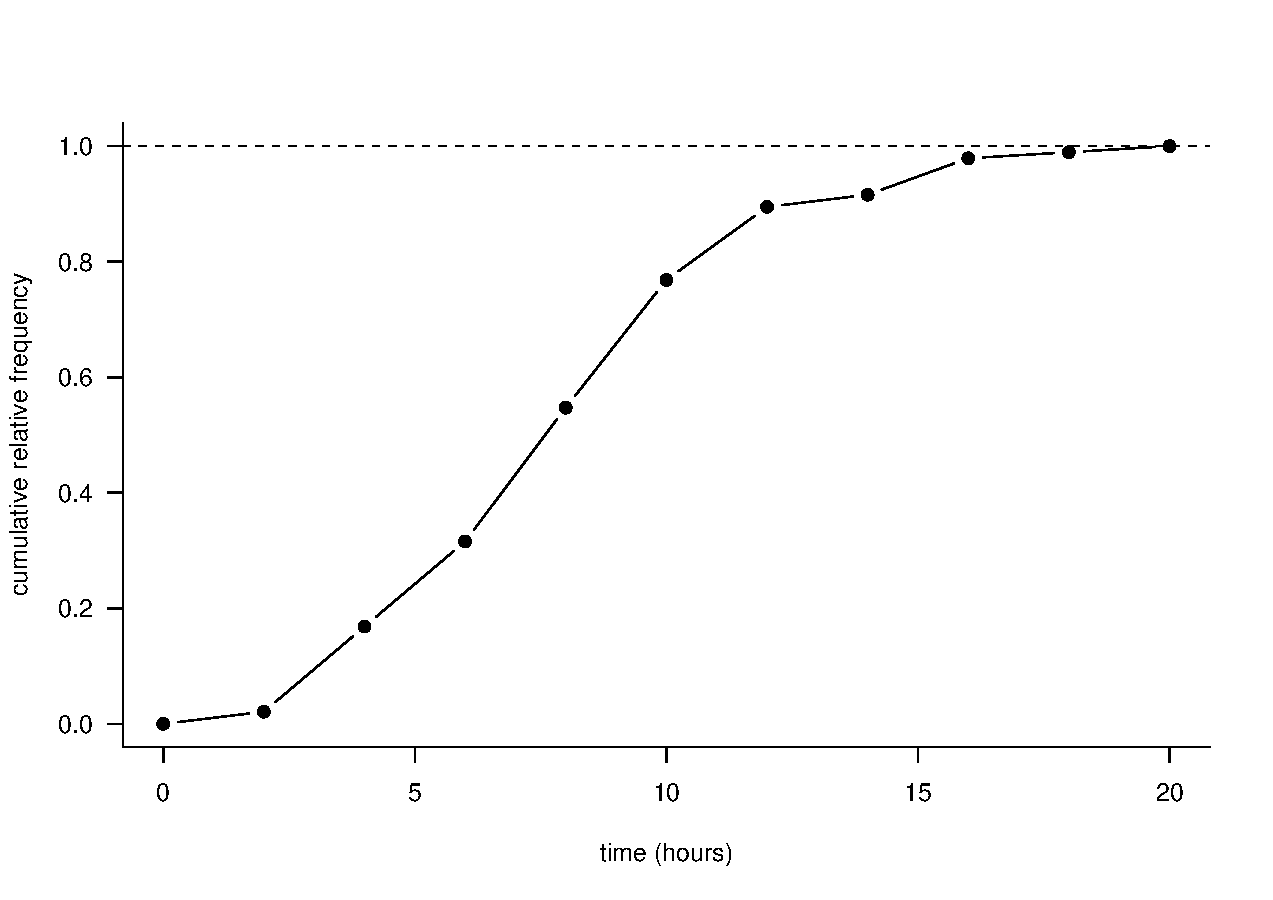
\includegraphics[width=0.75\linewidth]{images/ox_cum_freq} 

}

\caption{A cumulative relative frequency distribution of the Oxford birth times.}\label{fig:oxcumfreq}
\end{figure}

The shape of this plot depends on the choice of the classes. We could increase the detail in the plot by increasing the number of classes, that is, by decreasing the class width. In an extreme case we could choose the classes so that there is a class for every unique value in the data. Table \ref{tab:oxfreqecdf} shows how this could be done.



 
  \providecommand{\huxb}[2]{\arrayrulecolor[RGB]{#1}\global\arrayrulewidth=#2pt}
  \providecommand{\huxvb}[2]{\color[RGB]{#1}\vrule width #2pt}
  \providecommand{\huxtpad}[1]{\rule{0pt}{#1}}
  \providecommand{\huxbpad}[1]{\rule[-#1]{0pt}{#1}}

\begin{table}[ht]
\begin{centerbox}
\begin{threeparttable}
\captionsetup{justification=centering,singlelinecheck=off}
\caption{\label{tab:oxfreqecdf} Frequency table of the Oxford birth times, with one observation per class.}
 \setlength{\tabcolsep}{0pt}
\begin{tabularx}{0.8\textwidth}{p{0.16\textwidth} p{0.16\textwidth} p{0.16\textwidth} p{0.16\textwidth} p{0.16\textwidth}}


\hhline{>{\huxb{0, 0, 0}{1}}->{\huxb{0, 0, 0}{1}}->{\huxb{0, 0, 0}{1}}->{\huxb{0, 0, 0}{1}}->{\huxb{0, 0, 0}{1}}-}
\arrayrulecolor{black}

\multicolumn{1}{!{\huxvb{0, 0, 0}{0}}p{0.16\textwidth}!{\huxvb{0, 0, 0}{0}}}{\cellcolor[RGB]{255, 255, 255}\hspace{6pt}\parbox[b]{0.16\textwidth-6pt-6pt}{\huxtpad{0pt + 1em}\centering time (hours)\huxbpad{0pt}}} &
\multicolumn{1}{p{0.16\textwidth}!{\huxvb{0, 0, 0}{0}}}{\cellcolor[RGB]{255, 255, 255}\hspace{6pt}\parbox[b]{0.16\textwidth-6pt-6pt}{\huxtpad{0pt + 1em}\centering frequency\huxbpad{0pt}}} &
\multicolumn{1}{p{0.16\textwidth}!{\huxvb{0, 0, 0}{0}}}{\cellcolor[RGB]{255, 255, 255}\hspace{6pt}\parbox[b]{0.16\textwidth-6pt-6pt}{\huxtpad{0pt + 1em}\centering relative frequency\huxbpad{0pt}}} &
\multicolumn{1}{p{0.16\textwidth}!{\huxvb{0, 0, 0}{0}}}{\cellcolor[RGB]{255, 255, 255}\hspace{6pt}\parbox[b]{0.16\textwidth-6pt-6pt}{\huxtpad{0pt + 1em}\centering cumulative frequency\huxbpad{0pt}}} &
\multicolumn{1}{p{0.16\textwidth}!{\huxvb{0, 0, 0}{0}}}{\cellcolor[RGB]{255, 255, 255}\hspace{6pt}\parbox[b]{0.16\textwidth-6pt-6pt}{\huxtpad{0pt + 1em}\centering cumulative relative frequency\huxbpad{0pt}}} \tabularnewline[-0.5pt]


\hhline{>{\huxb{0, 0, 0}{1}}->{\huxb{0, 0, 0}{1}}->{\huxb{0, 0, 0}{1}}->{\huxb{0, 0, 0}{1}}->{\huxb{0, 0, 0}{1}}-}
\arrayrulecolor{black}

\multicolumn{1}{!{\huxvb{0, 0, 0}{0}}p{0.16\textwidth}!{\huxvb{0, 0, 0}{0}}}{\cellcolor[RGB]{255, 255, 255}\hspace{6pt}\parbox[b]{0.16\textwidth-6pt-6pt}{\huxtpad{0pt + 1em}\centering 0.0-1.5\huxbpad{0pt}}} &
\multicolumn{1}{p{0.16\textwidth}!{\huxvb{0, 0, 0}{0}}}{\cellcolor[RGB]{255, 255, 255}\hspace{6pt}\parbox[b]{0.16\textwidth-6pt-6pt}{\huxtpad{0pt + 1em}\centering 1\huxbpad{0pt}}} &
\multicolumn{1}{p{0.16\textwidth}!{\huxvb{0, 0, 0}{0}}}{\cellcolor[RGB]{255, 255, 255}\hspace{6pt}\parbox[b]{0.16\textwidth-6pt-6pt}{\huxtpad{0pt + 1em}\centering 1/95\huxbpad{0pt}}} &
\multicolumn{1}{p{0.16\textwidth}!{\huxvb{0, 0, 0}{0}}}{\cellcolor[RGB]{255, 255, 255}\hspace{6pt}\parbox[b]{0.16\textwidth-6pt-6pt}{\huxtpad{0pt + 1em}\centering 1\huxbpad{0pt}}} &
\multicolumn{1}{p{0.16\textwidth}!{\huxvb{0, 0, 0}{0}}}{\cellcolor[RGB]{255, 255, 255}\hspace{6pt}\parbox[b]{0.16\textwidth-6pt-6pt}{\huxtpad{0pt + 1em}\centering 1/95\huxbpad{0pt}}} \tabularnewline[-0.5pt]


\hhline{>{\huxb{255, 255, 255}{0.1}}->{\huxb{255, 255, 255}{0.1}}->{\huxb{255, 255, 255}{0.1}}->{\huxb{255, 255, 255}{0.1}}->{\huxb{255, 255, 255}{0.1}}-}
\arrayrulecolor{black}

\multicolumn{1}{!{\huxvb{0, 0, 0}{0}}p{0.16\textwidth}!{\huxvb{0, 0, 0}{0}}}{\cellcolor[RGB]{255, 255, 255}\hspace{6pt}\parbox[b]{0.16\textwidth-6pt-6pt}{\huxtpad{0pt + 1em}\centering 1.5-2.0\huxbpad{0pt}}} &
\multicolumn{1}{p{0.16\textwidth}!{\huxvb{0, 0, 0}{0}}}{\cellcolor[RGB]{255, 255, 255}\hspace{6pt}\parbox[b]{0.16\textwidth-6pt-6pt}{\huxtpad{0pt + 1em}\centering 1\huxbpad{0pt}}} &
\multicolumn{1}{p{0.16\textwidth}!{\huxvb{0, 0, 0}{0}}}{\cellcolor[RGB]{255, 255, 255}\hspace{6pt}\parbox[b]{0.16\textwidth-6pt-6pt}{\huxtpad{0pt + 1em}\centering 1/95\huxbpad{0pt}}} &
\multicolumn{1}{p{0.16\textwidth}!{\huxvb{0, 0, 0}{0}}}{\cellcolor[RGB]{255, 255, 255}\hspace{6pt}\parbox[b]{0.16\textwidth-6pt-6pt}{\huxtpad{0pt + 1em}\centering 2\huxbpad{0pt}}} &
\multicolumn{1}{p{0.16\textwidth}!{\huxvb{0, 0, 0}{0}}}{\cellcolor[RGB]{255, 255, 255}\hspace{6pt}\parbox[b]{0.16\textwidth-6pt-6pt}{\huxtpad{0pt + 1em}\centering 2/95\huxbpad{0pt}}} \tabularnewline[-0.5pt]


\hhline{>{\huxb{255, 255, 255}{0.1}}->{\huxb{255, 255, 255}{0.1}}->{\huxb{255, 255, 255}{0.1}}->{\huxb{255, 255, 255}{0.1}}->{\huxb{255, 255, 255}{0.1}}-}
\arrayrulecolor{black}

\multicolumn{1}{!{\huxvb{0, 0, 0}{0}}p{0.16\textwidth}!{\huxvb{0, 0, 0}{0}}}{\cellcolor[RGB]{255, 255, 255}\hspace{6pt}\parbox[b]{0.16\textwidth-6pt-6pt}{\huxtpad{0pt + 1em}\centering 2.0-2.1\huxbpad{0pt}}} &
\multicolumn{1}{p{0.16\textwidth}!{\huxvb{0, 0, 0}{0}}}{\cellcolor[RGB]{255, 255, 255}\hspace{6pt}\parbox[b]{0.16\textwidth-6pt-6pt}{\huxtpad{0pt + 1em}\centering 1\huxbpad{0pt}}} &
\multicolumn{1}{p{0.16\textwidth}!{\huxvb{0, 0, 0}{0}}}{\cellcolor[RGB]{255, 255, 255}\hspace{6pt}\parbox[b]{0.16\textwidth-6pt-6pt}{\huxtpad{0pt + 1em}\centering 1/95\huxbpad{0pt}}} &
\multicolumn{1}{p{0.16\textwidth}!{\huxvb{0, 0, 0}{0}}}{\cellcolor[RGB]{255, 255, 255}\hspace{6pt}\parbox[b]{0.16\textwidth-6pt-6pt}{\huxtpad{0pt + 1em}\centering 3\huxbpad{0pt}}} &
\multicolumn{1}{p{0.16\textwidth}!{\huxvb{0, 0, 0}{0}}}{\cellcolor[RGB]{255, 255, 255}\hspace{6pt}\parbox[b]{0.16\textwidth-6pt-6pt}{\huxtpad{0pt + 1em}\centering 3/95\huxbpad{0pt}}} \tabularnewline[-0.5pt]


\hhline{>{\huxb{255, 255, 255}{0.1}}->{\huxb{255, 255, 255}{0.1}}->{\huxb{255, 255, 255}{0.1}}->{\huxb{255, 255, 255}{0.1}}->{\huxb{255, 255, 255}{0.1}}-}
\arrayrulecolor{black}

\multicolumn{1}{!{\huxvb{0, 0, 0}{0}}p{0.16\textwidth}!{\huxvb{0, 0, 0}{0}}}{\cellcolor[RGB]{255, 255, 255}\hspace{6pt}\parbox[b]{0.16\textwidth-6pt-6pt}{\huxtpad{0pt + 1em}\centering 2.1-2.5\huxbpad{0pt}}} &
\multicolumn{1}{p{0.16\textwidth}!{\huxvb{0, 0, 0}{0}}}{\cellcolor[RGB]{255, 255, 255}\hspace{6pt}\parbox[b]{0.16\textwidth-6pt-6pt}{\huxtpad{0pt + 1em}\centering 2\huxbpad{0pt}}} &
\multicolumn{1}{p{0.16\textwidth}!{\huxvb{0, 0, 0}{0}}}{\cellcolor[RGB]{255, 255, 255}\hspace{6pt}\parbox[b]{0.16\textwidth-6pt-6pt}{\huxtpad{0pt + 1em}\centering 2/95\huxbpad{0pt}}} &
\multicolumn{1}{p{0.16\textwidth}!{\huxvb{0, 0, 0}{0}}}{\cellcolor[RGB]{255, 255, 255}\hspace{6pt}\parbox[b]{0.16\textwidth-6pt-6pt}{\huxtpad{0pt + 1em}\centering 5\huxbpad{0pt}}} &
\multicolumn{1}{p{0.16\textwidth}!{\huxvb{0, 0, 0}{0}}}{\cellcolor[RGB]{255, 255, 255}\hspace{6pt}\parbox[b]{0.16\textwidth-6pt-6pt}{\huxtpad{0pt + 1em}\centering 5/95\huxbpad{0pt}}} \tabularnewline[-0.5pt]


\hhline{>{\huxb{255, 255, 255}{0.1}}->{\huxb{255, 255, 255}{0.1}}->{\huxb{255, 255, 255}{0.1}}->{\huxb{255, 255, 255}{0.1}}->{\huxb{255, 255, 255}{0.1}}-}
\arrayrulecolor{black}

\multicolumn{1}{!{\huxvb{0, 0, 0}{0}}p{0.16\textwidth}!{\huxvb{0, 0, 0}{0}}}{\cellcolor[RGB]{255, 255, 255}\hspace{6pt}\parbox[b]{0.16\textwidth-6pt-6pt}{\huxtpad{0pt + 1em}\centering ...\huxbpad{0pt}}} &
\multicolumn{1}{p{0.16\textwidth}!{\huxvb{0, 0, 0}{0}}}{\cellcolor[RGB]{255, 255, 255}\hspace{6pt}\parbox[b]{0.16\textwidth-6pt-6pt}{\huxtpad{0pt + 1em}\centering ...\huxbpad{0pt}}} &
\multicolumn{1}{p{0.16\textwidth}!{\huxvb{0, 0, 0}{0}}}{\cellcolor[RGB]{255, 255, 255}\hspace{6pt}\parbox[b]{0.16\textwidth-6pt-6pt}{\huxtpad{0pt + 1em}\centering ...\huxbpad{0pt}}} &
\multicolumn{1}{p{0.16\textwidth}!{\huxvb{0, 0, 0}{0}}}{\cellcolor[RGB]{255, 255, 255}\hspace{6pt}\parbox[b]{0.16\textwidth-6pt-6pt}{\huxtpad{0pt + 1em}\centering ...\huxbpad{0pt}}} &
\multicolumn{1}{p{0.16\textwidth}!{\huxvb{0, 0, 0}{0}}}{\cellcolor[RGB]{255, 255, 255}\hspace{6pt}\parbox[b]{0.16\textwidth-6pt-6pt}{\huxtpad{0pt + 1em}\centering ...\huxbpad{0pt}}} \tabularnewline[-0.5pt]


\hhline{>{\huxb{255, 255, 255}{0.1}}->{\huxb{255, 255, 255}{0.1}}->{\huxb{255, 255, 255}{0.1}}->{\huxb{255, 255, 255}{0.1}}->{\huxb{255, 255, 255}{0.1}}-}
\arrayrulecolor{black}

\multicolumn{1}{!{\huxvb{0, 0, 0}{0}}p{0.16\textwidth}!{\huxvb{0, 0, 0}{0}}}{\cellcolor[RGB]{255, 255, 255}\hspace{6pt}\parbox[b]{0.16\textwidth-6pt-6pt}{\huxtpad{0pt + 1em}\centering 16.0-16.5\huxbpad{0pt}}} &
\multicolumn{1}{p{0.16\textwidth}!{\huxvb{0, 0, 0}{0}}}{\cellcolor[RGB]{255, 255, 255}\hspace{6pt}\parbox[b]{0.16\textwidth-6pt-6pt}{\huxtpad{0pt + 1em}\centering 1\huxbpad{0pt}}} &
\multicolumn{1}{p{0.16\textwidth}!{\huxvb{0, 0, 0}{0}}}{\cellcolor[RGB]{255, 255, 255}\hspace{6pt}\parbox[b]{0.16\textwidth-6pt-6pt}{\huxtpad{0pt + 1em}\centering 1/95\huxbpad{0pt}}} &
\multicolumn{1}{p{0.16\textwidth}!{\huxvb{0, 0, 0}{0}}}{\cellcolor[RGB]{255, 255, 255}\hspace{6pt}\parbox[b]{0.16\textwidth-6pt-6pt}{\huxtpad{0pt + 1em}\centering 94\huxbpad{0pt}}} &
\multicolumn{1}{p{0.16\textwidth}!{\huxvb{0, 0, 0}{0}}}{\cellcolor[RGB]{255, 255, 255}\hspace{6pt}\parbox[b]{0.16\textwidth-6pt-6pt}{\huxtpad{0pt + 1em}\centering 94/95\huxbpad{0pt}}} \tabularnewline[-0.5pt]


\hhline{>{\huxb{255, 255, 255}{0.1}}->{\huxb{255, 255, 255}{0.1}}->{\huxb{255, 255, 255}{0.1}}->{\huxb{255, 255, 255}{0.1}}->{\huxb{255, 255, 255}{0.1}}-}
\arrayrulecolor{black}

\multicolumn{1}{!{\huxvb{0, 0, 0}{0}}p{0.16\textwidth}!{\huxvb{0, 0, 0}{0}}}{\cellcolor[RGB]{255, 255, 255}\hspace{6pt}\parbox[b]{0.16\textwidth-6pt-6pt}{\huxtpad{0pt + 1em}\centering 16.5-19.0\huxbpad{0pt}}} &
\multicolumn{1}{p{0.16\textwidth}!{\huxvb{0, 0, 0}{0}}}{\cellcolor[RGB]{255, 255, 255}\hspace{6pt}\parbox[b]{0.16\textwidth-6pt-6pt}{\huxtpad{0pt + 1em}\centering 1\huxbpad{0pt}}} &
\multicolumn{1}{p{0.16\textwidth}!{\huxvb{0, 0, 0}{0}}}{\cellcolor[RGB]{255, 255, 255}\hspace{6pt}\parbox[b]{0.16\textwidth-6pt-6pt}{\huxtpad{0pt + 1em}\centering 1/95\huxbpad{0pt}}} &
\multicolumn{1}{p{0.16\textwidth}!{\huxvb{0, 0, 0}{0}}}{\cellcolor[RGB]{255, 255, 255}\hspace{6pt}\parbox[b]{0.16\textwidth-6pt-6pt}{\huxtpad{0pt + 1em}\centering 95\huxbpad{0pt}}} &
\multicolumn{1}{p{0.16\textwidth}!{\huxvb{0, 0, 0}{0}}}{\cellcolor[RGB]{255, 255, 255}\hspace{6pt}\parbox[b]{0.16\textwidth-6pt-6pt}{\huxtpad{0pt + 1em}\centering 1\huxbpad{0pt}}} \tabularnewline[-0.5pt]


\hhline{>{\huxb{0, 0, 0}{1}}->{\huxb{0, 0, 0}{1}}->{\huxb{0, 0, 0}{1}}->{\huxb{0, 0, 0}{1}}->{\huxb{0, 0, 0}{1}}-}
\arrayrulecolor{black}

\multicolumn{1}{!{\huxvb{0, 0, 0}{0}}p{0.16\textwidth}!{\huxvb{0, 0, 0}{0}}}{\cellcolor[RGB]{255, 255, 255}\hspace{6pt}\parbox[b]{0.16\textwidth-6pt-6pt}{\huxtpad{0pt + 1em}\centering total\huxbpad{0pt}}} &
\multicolumn{1}{p{0.16\textwidth}!{\huxvb{0, 0, 0}{0}}}{\cellcolor[RGB]{255, 255, 255}\hspace{6pt}\parbox[b]{0.16\textwidth-6pt-6pt}{\huxtpad{0pt + 1em}\centering 95\huxbpad{0pt}}} &
\multicolumn{1}{p{0.16\textwidth}!{\huxvb{0, 0, 0}{0}}}{\cellcolor[RGB]{255, 255, 255}\hspace{6pt}\parbox[b]{0.16\textwidth-6pt-6pt}{\huxtpad{0pt + 1em}\centering 1\huxbpad{0pt}}} &
\multicolumn{1}{p{0.16\textwidth}!{\huxvb{0, 0, 0}{0}}}{\cellcolor[RGB]{255, 255, 255}\hspace{6pt}\parbox[b]{0.16\textwidth-6pt-6pt}{\huxtpad{0pt + 1em}\centering \huxbpad{0pt}}} &
\multicolumn{1}{p{0.16\textwidth}!{\huxvb{0, 0, 0}{0}}}{\cellcolor[RGB]{255, 255, 255}\hspace{6pt}\parbox[b]{0.16\textwidth-6pt-6pt}{\huxtpad{0pt + 1em}\centering \huxbpad{0pt}}} \tabularnewline[-0.5pt]


\hhline{}
\arrayrulecolor{black}
\end{tabularx}
\end{threeparttable}\par\end{centerbox}

\end{table}
 

Figure \ref{fig:oxcumfreq2} shows the resulting graph. Notice that the shape is similar to Figure \ref{fig:oxcumfreq} but it is less smooth. The function (from time on the horizontal axis to cumulative relative frequency on the vertical axis) is often called the \textbf{empirical cumulative distribution function} or \textbf{empirical c.d.f}. The meaning will become clearer when we look at c.d.f.s in Section \ref{discrete}.

\begin{figure}

{\centering \includegraphics[width=0.75\linewidth]{images/ox_cum_freq2new} 

}

\caption{A cumulative relative frequency distribution of the Oxford birth times, with classes defined so that there is one data value in each class.}\label{fig:oxcumfreq2}
\end{figure}

Sometimes data are given to us in the form of Table \ref{tab:oxfreq} and the individual data values are not available. For example, some birth data published by the Office of National Statistics data give mother's age in 5 year age bands. Data provided in this form are called \textbf{grouped data}. We will analyse data from tables in Chapter \ref{contingency}.

\hypertarget{graphs}{%
\section{Graphs (1 variable)}\label{graphs}}

These days it is very easy to plot a graph using a computer. However, \textbf{you} need to decide which type of graph is appropriate and the default graph produced by the computer may not be very good. Some general rules:

\begin{itemize}
\tightlist
\item
  \textbf{Always plot the data}. Often this will show clearly the important features of the data. Formal statistical methods may be unnecessary or simply confirm the visual impression given by the plot. Also, plotting the data can reveal potential problems with the data, for example, outlying observations which do not fit in the with the general pattern of the data, or data which are clearly wrong.
\item
  For datasets with more than one variable always plot the variables against
  each other. There may be observations which are not unusual when variables are considered separately but are clearly unusual when 2 variables are plotted. See Section \ref{graphs2}.
\item
  A good graph draws attention to important aspects of the data. Anything which distracts the viewer, for example, excessive shading, symbols, 3-dimensional effects, should be removed.\\
\item
  Axis labels (remember the units!), the legend and caption should enable the viewer of the graph to understand the content of the graph.
\end{itemize}

\hypertarget{histogram}{%
\subsection{Histograms}\label{histogram}}

A \textbf{histogram} is a graphical display based on the relative frequency distribution of a set of data on a \textbf{continuous} variable. The variable of interest is plotted on the \(x\)-axis, which is divided into \textbf{bins} based on the classes of the frequency distribution. A rectangle is plotted for each bin. The height of a rectangle is calculated as
\begin{equation}
\mbox{height} = \frac{\mbox{relative frequency}}{\mbox{bin width}} = \frac{\mbox{frequency}}{n \times \mbox{bin width}}.
\label{eq:hist}
\end{equation}
Therefore, for a given box in the histogram:

\begin{itemize}
\tightlist
\item
  the \textbf{area} represents the relative frequency of the observations in
  the interval;
\item
  the \textbf{height} represents the relative frequency of the observations in
  the interval \textbf{per unit of measurement}, commonly known as the \textbf{density}.
\end{itemize}

The total area under a histogram is equal to 1. In fact a histogram is an estimate of a probability density function (see Section \ref{continuous}). The vertical axis is commonly labelled \textbf{density}.

It is common for people to plot frequencies (rather than relative frequencies per unit), giving what I will call a \textbf{frequency plot}, that is, \textbf{not} a true histogram.

If the bin widths are equal the shape of frequency plot is the same as the corresponding histogram. However, when drawing a frequency plot using unequal bin widths it is important to take into account the differing widths of the bins. For example, in the plot on the bottom left of Figure \ref{fig:oxhistbasic}, the frequency in the box for 12-20 hours is 4 times too high because the longer width of this interval has not been taken into account.
One solution is to divide the frequencies by the bin width to produce frequencies \textbf{per unit}, but then we may as well produce a true histogram, using equation \eqref{eq:hist}.

\begin{figure}

{\centering \includegraphics[width=0.75\linewidth]{images/ox_hist_basic} 

}

\caption{Frequency plots (left) and histograms (right) of the Oxford birth times.}\label{fig:oxhistbasic}
\end{figure}

A histogram can be useful to look at the shape of a distribution. However,
especially for a small dataset, the shape of the histogram can depend greatly on the classes chosen to define the bins. Figure \ref{fig:oxhistbasic} contains histograms and frequency histograms of the all the times in Table \ref{tab:taboxbirths}. From the histograms we can easily see that the birth times data are slightly positively skewed.

\hypertarget{stem}{%
\subsection{Stem-and-leaf plots}\label{stem}}

A \textbf{stem-and-leaf plot} (or stem plot) is like an enhanced histogram. The \textbf{stem}, on the left, contain the times in whole hours. The \textbf{leaves},
on the right, contain the first digit after the decimal point. An advantage of a stem-and-leaf plot is that it gives the entire dataset (perhaps rounded) in sorted order. It is easy to calculate the five number summary of the data from a stem-and-leaf plot. Figure \ref{fig:oxstem} shows a stem-and-leaf plot of the Oxford births data.

\begin{figure}

{\centering \includegraphics[width=0.6\linewidth]{images/ox_stem} 

}

\caption{Stem-and-leaf plot of the Oxford birth times. The decimal point is at the vertical line |. The data are rounded to the nearest 0.1 before plotting.}\label{fig:oxstem}
\end{figure}

\hypertarget{dotplots}{%
\subsection{Dotplots}\label{dotplots}}

Dotplots are simple plots in which each observation is represented by a dot. If there are repeated observations, that is, observations with the same value (perhaps after rounding), then their dots are stacked on top of each other. Figure \ref{fig:oxdotbasic} shows two dotplots. In the right hand plot the data were rounded to the nearest hour, producing a plot that looks a bit like a histogram with a bin width of 1 hour, with rectangles replaced by vertical lines of dots.

\begin{figure}

{\centering 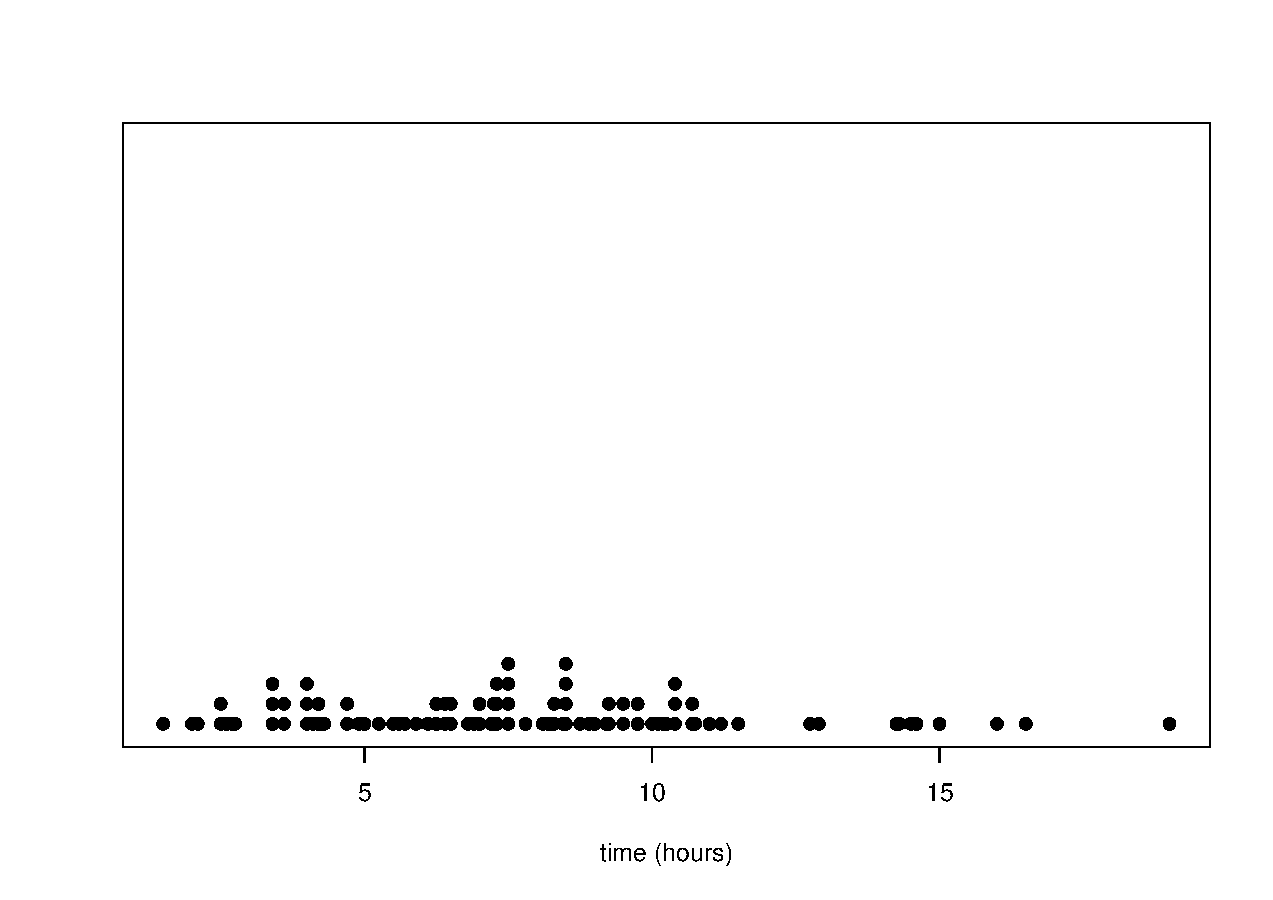
\includegraphics[width=0.75\linewidth]{images/ox_dot_basic} 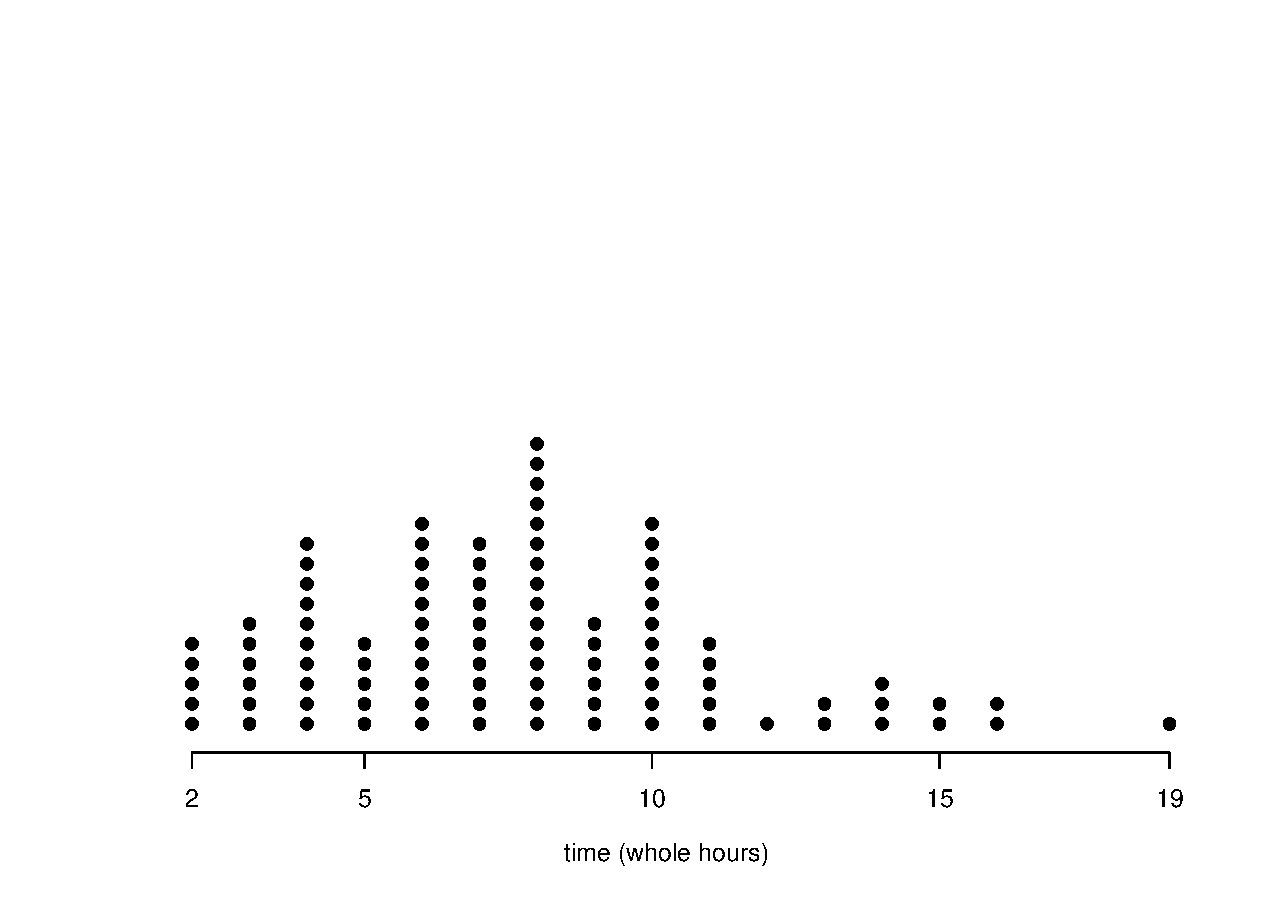
\includegraphics[width=0.75\linewidth]{images/ox_dot_adv} 

}

\caption{Dotplots of the Oxford birth times. Top: raw data (and lots of wasted white space).  Bottom: data rounded to the nearest hour.}\label{fig:oxdotbasic}
\end{figure}

\hypertarget{boxplots}{%
\subsection{Boxplots}\label{boxplots}}

A \textbf{boxplot} (or box-and-whisker plot) is a graphical display containing the five-number summary. It also provides ways to assess the overall shape of the data. Figure \ref{fig:oxdotbasic} explains how a standard boxplot is constructed.

\begin{figure}

{\centering 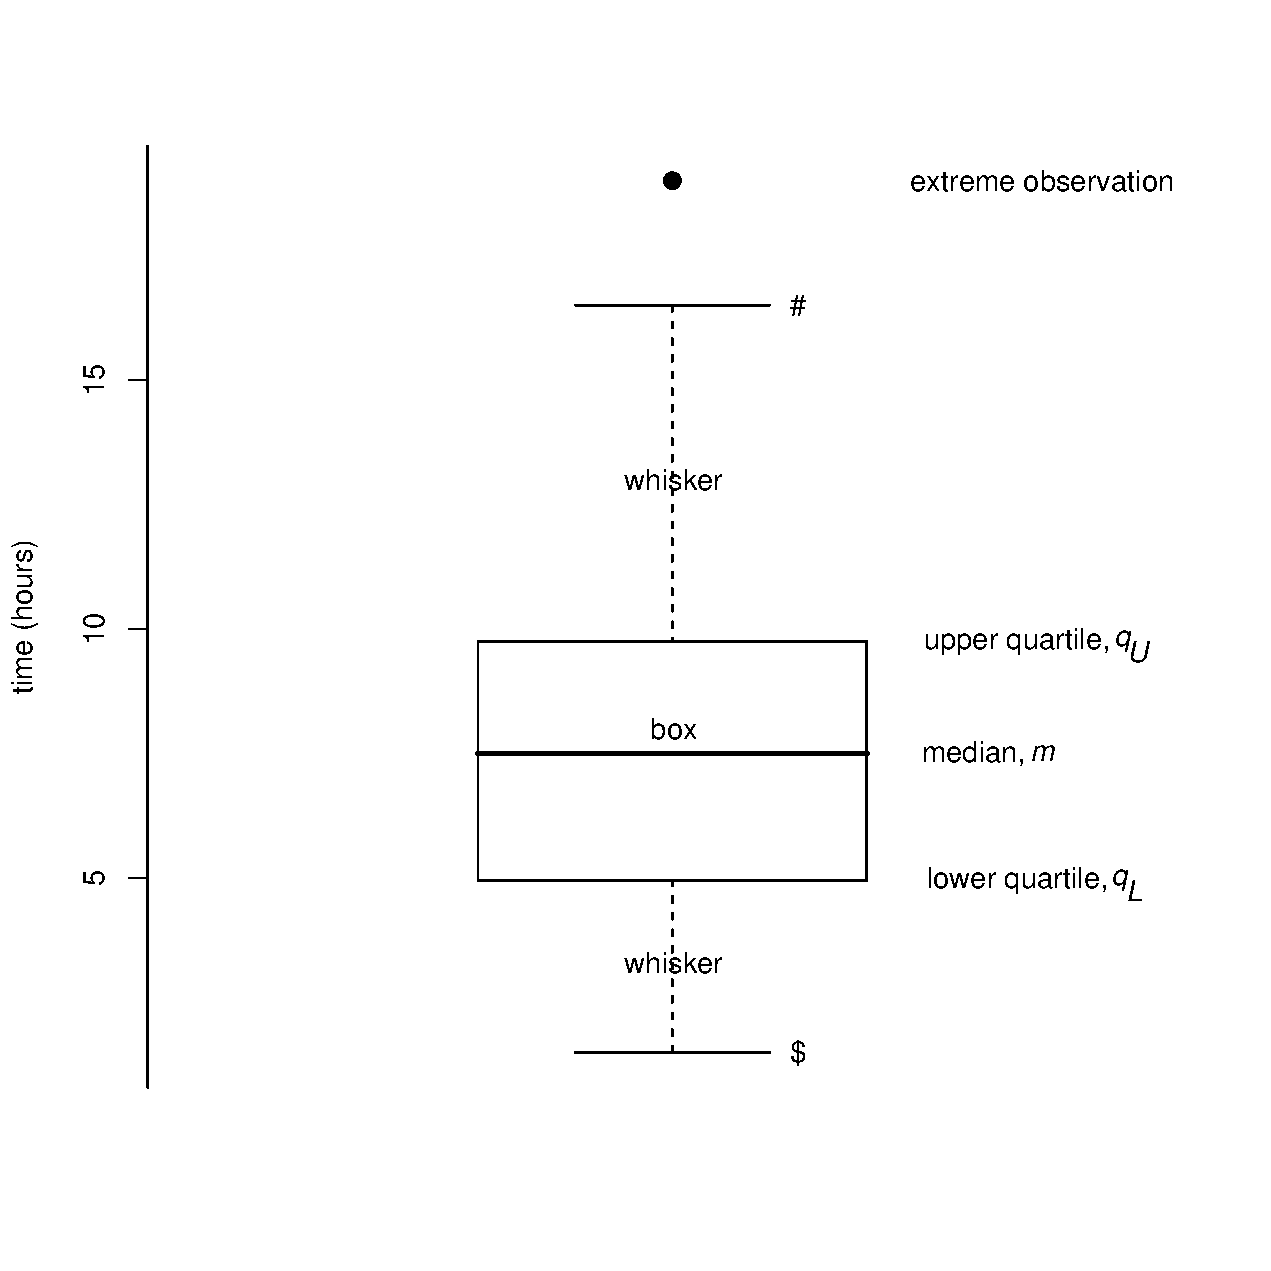
\includegraphics[width=0.75\linewidth]{images/ox_box_basic} 

}

\caption{Boxplot of the Oxford birth times. The upper end (\#) of the upper whisker is drawn at the largest observation within a distance $1.5 (q_U-q_L)$ of $q_U$. The lower end (\$) of the lower whisker is drawn at the smallest observation within a distance $1.5 (q_U-q_L)$ of $q_L$.}\label{fig:oxboxbasic}
\end{figure}

The `box' shows where 50\% of the data lie, that is, between the lower and uper
quartiles. The `whiskers' extend to the most extreme observations that are within 1.5 IQR of the ends of the box. Sometimes a different criterion is used to determine the ends of the whiskers. Any more extreme values are individually identified (with a dot here).

It can less easy easy to come to a conclusion concerning the nature of skewness using a boxplot than using a histogram. In this example the lengths of the whiskers and the presence of the value at 19 hours suggest slight positive skewness. However, the relative positions of the samples quartiles suggest (very slight) negative skewness, which is the cause of the slightly negative value of sample quartiles skewness towards the end of Section \ref{symmetry}.

Some alternatives are given in Figure \ref{fig:oxboxadv}. Which do you prefer?

\begin{figure}

{\centering 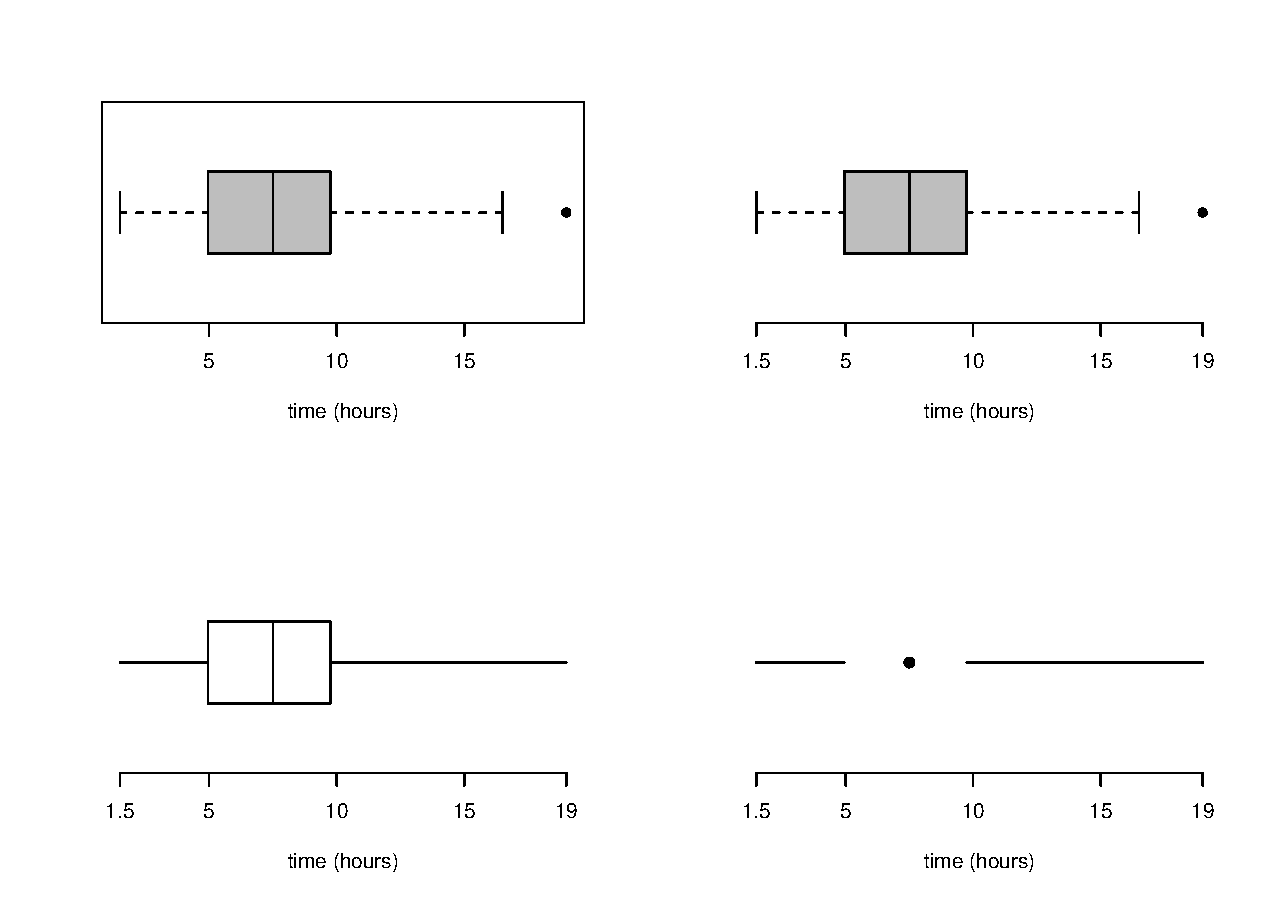
\includegraphics[width=0.75\linewidth]{images/ox_box_adv} 

}

\caption{Alternative plots of the Oxford birth times based on the five-figure summary.}\label{fig:oxboxadv}
\end{figure}

\hypertarget{barplots}{%
\subsection{Barplots}\label{barplots}}

A \textbf{barplot} (or bar chart) has a similar appearance to a histogram but is used for numerical discrete data or categorical data. Therefore there are gaps between the bars in a barplot.

\hypertarget{example-numerical-discrete-data}{%
\subsubsection*{Example: numerical discrete data}\label{example-numerical-discrete-data}}
\addcontentsline{toc}{subsubsection}{Example: numerical discrete data}

Table \ref{tab:shuttlenew} shows the frequencies of the number of damaged O-rings in the space shuttle example. Figure \ref{fig:shuttlebarplots} shows barplots (or equivalent) of these data. Which do you prefer?

\begin{table}

\caption{\label{tab:shuttlenew}Frequencies of numbers of damaged O-rings for the space shuttle data.}
\centering
\begin{tabular}[t]{lllll}
\toprule
number of damaged O-rings & 0 & 1 & 2 & 3\\
frequency & 16 & 5 & 1 & 1\\
\bottomrule
\end{tabular}
\end{table}

\begin{figure}

{\centering 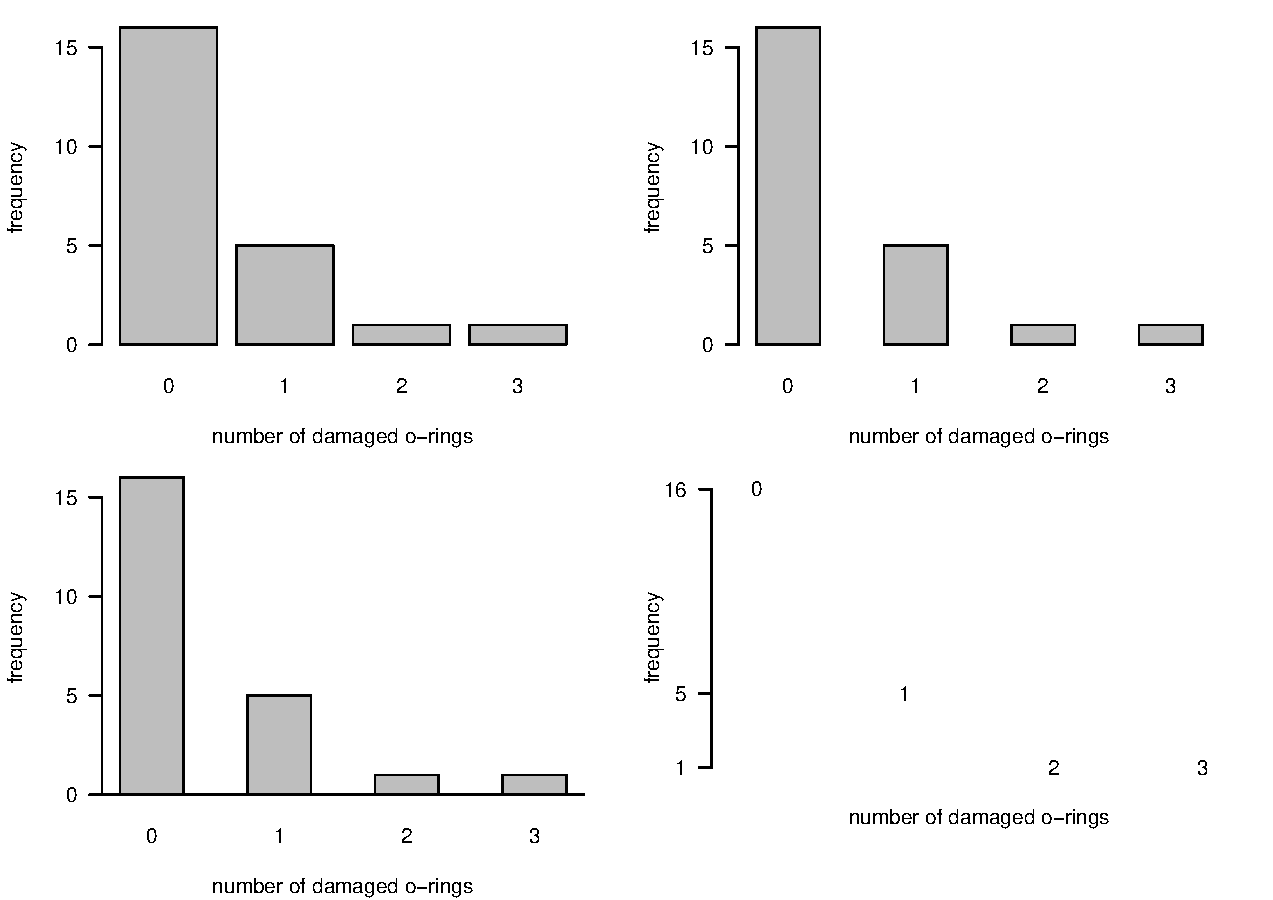
\includegraphics[width=0.75\linewidth]{images/shuttle_barplots} 

}

\caption{Barplots of numbers of damaged O-rings on space shuttle flights.}\label{fig:shuttlebarplots}
\end{figure}

\hypertarget{example-categorical-data}{%
\subsubsection*{Example: categorical data}\label{example-categorical-data}}
\addcontentsline{toc}{subsubsection}{Example: categorical data}

Table \ref{tab:ABOnew} shows the percentages of people in the UK with the 8 main blood groups O\(+\), A\(+\), B\(+\), AB\(+\), O\(-\), A\(-\), B\(-\) and AB\(-\). See section \ref{bloodindep} for more details about blood groups. These data are nominal.

 
  \providecommand{\huxb}[2]{\arrayrulecolor[RGB]{#1}\global\arrayrulewidth=#2pt}
  \providecommand{\huxvb}[2]{\color[RGB]{#1}\vrule width #2pt}
  \providecommand{\huxtpad}[1]{\rule{0pt}{#1}}
  \providecommand{\huxbpad}[1]{\rule[-#1]{0pt}{#1}}

\begin{table}[ht]
\begin{centerbox}
\begin{threeparttable}
\captionsetup{justification=centering,singlelinecheck=off}
\caption{\label{tab:ABOnew} Percentages of people in the UK with the 8 main blood groups}
 \setlength{\tabcolsep}{0pt}
\begin{tabularx}{0.8\textwidth}{p{0.2\textwidth} p{0.2\textwidth} p{0.2\textwidth} p{0.2\textwidth}}


\hhline{>{\huxb{255, 255, 255}{0.1}}->{\huxb{255, 255, 255}{0.1}}->{\huxb{255, 255, 255}{0.1}}->{\huxb{255, 255, 255}{0.1}}-}
\arrayrulecolor{black}

\multicolumn{1}{!{\huxvb{0, 0, 0}{0}}p{0.2\textwidth}!{\huxvb{0, 0, 0}{1}}}{\cellcolor[RGB]{255, 255, 255}\hspace{6pt}\parbox[b]{0.2\textwidth-6pt-6pt}{\huxtpad{6pt + 1em}\centering blood type\huxbpad{6pt}}} &
\multicolumn{1}{p{0.2\textwidth}!{\huxvb{0, 0, 0}{0}}}{\cellcolor[RGB]{255, 255, 255}\hspace{6pt}\parbox[b]{0.2\textwidth-6pt-6pt}{\huxtpad{6pt + 1em}\centering Rh+\huxbpad{6pt}}} &
\multicolumn{1}{p{0.2\textwidth}!{\huxvb{0, 0, 0}{1}}}{\cellcolor[RGB]{255, 255, 255}\hspace{6pt}\parbox[b]{0.2\textwidth-6pt-6pt}{\huxtpad{6pt + 1em}\centering Rh-\huxbpad{6pt}}} &
\multicolumn{1}{p{0.2\textwidth}!{\huxvb{0, 0, 0}{0}}}{\cellcolor[RGB]{255, 255, 255}\hspace{6pt}\parbox[b]{0.2\textwidth-6pt-6pt}{\huxtpad{6pt + 1em}\centering total\huxbpad{6pt}}} \tabularnewline[-0.5pt]


\hhline{>{\huxb{0, 0, 0}{1}}->{\huxb{0, 0, 0}{1}}->{\huxb{0, 0, 0}{1}}->{\huxb{0, 0, 0}{1}}-}
\arrayrulecolor{black}

\multicolumn{1}{!{\huxvb{0, 0, 0}{0}}p{0.2\textwidth}!{\huxvb{0, 0, 0}{1}}}{\cellcolor[RGB]{255, 255, 255}\hspace{6pt}\parbox[b]{0.2\textwidth-6pt-6pt}{\huxtpad{6pt + 1em}\centering O\huxbpad{6pt}}} &
\multicolumn{1}{p{0.2\textwidth}!{\huxvb{0, 0, 0}{0}}}{\cellcolor[RGB]{255, 255, 255}\hspace{6pt}\parbox[b]{0.2\textwidth-6pt-6pt}{\huxtpad{6pt + 1em}\centering 37\huxbpad{6pt}}} &
\multicolumn{1}{p{0.2\textwidth}!{\huxvb{0, 0, 0}{1}}}{\cellcolor[RGB]{255, 255, 255}\hspace{6pt}\parbox[b]{0.2\textwidth-6pt-6pt}{\huxtpad{6pt + 1em}\centering 7\huxbpad{6pt}}} &
\multicolumn{1}{p{0.2\textwidth}!{\huxvb{0, 0, 0}{0}}}{\cellcolor[RGB]{255, 255, 255}\hspace{6pt}\parbox[b]{0.2\textwidth-6pt-6pt}{\huxtpad{6pt + 1em}\centering 44\huxbpad{6pt}}} \tabularnewline[-0.5pt]


\hhline{>{\huxb{255, 255, 255}{0.1}}->{\huxb{255, 255, 255}{0.1}}->{\huxb{255, 255, 255}{0.1}}->{\huxb{255, 255, 255}{0.1}}-}
\arrayrulecolor{black}

\multicolumn{1}{!{\huxvb{0, 0, 0}{0}}p{0.2\textwidth}!{\huxvb{0, 0, 0}{1}}}{\cellcolor[RGB]{255, 255, 255}\hspace{6pt}\parbox[b]{0.2\textwidth-6pt-6pt}{\huxtpad{6pt + 1em}\centering A\huxbpad{6pt}}} &
\multicolumn{1}{p{0.2\textwidth}!{\huxvb{0, 0, 0}{0}}}{\cellcolor[RGB]{255, 255, 255}\hspace{6pt}\parbox[b]{0.2\textwidth-6pt-6pt}{\huxtpad{6pt + 1em}\centering 35\huxbpad{6pt}}} &
\multicolumn{1}{p{0.2\textwidth}!{\huxvb{0, 0, 0}{1}}}{\cellcolor[RGB]{255, 255, 255}\hspace{6pt}\parbox[b]{0.2\textwidth-6pt-6pt}{\huxtpad{6pt + 1em}\centering 7\huxbpad{6pt}}} &
\multicolumn{1}{p{0.2\textwidth}!{\huxvb{0, 0, 0}{0}}}{\cellcolor[RGB]{255, 255, 255}\hspace{6pt}\parbox[b]{0.2\textwidth-6pt-6pt}{\huxtpad{6pt + 1em}\centering 42\huxbpad{6pt}}} \tabularnewline[-0.5pt]


\hhline{>{\huxb{255, 255, 255}{0.1}}->{\huxb{255, 255, 255}{0.1}}->{\huxb{255, 255, 255}{0.1}}->{\huxb{255, 255, 255}{0.1}}-}
\arrayrulecolor{black}

\multicolumn{1}{!{\huxvb{0, 0, 0}{0}}p{0.2\textwidth}!{\huxvb{0, 0, 0}{1}}}{\cellcolor[RGB]{255, 255, 255}\hspace{6pt}\parbox[b]{0.2\textwidth-6pt-6pt}{\huxtpad{6pt + 1em}\centering B\huxbpad{6pt}}} &
\multicolumn{1}{p{0.2\textwidth}!{\huxvb{0, 0, 0}{0}}}{\cellcolor[RGB]{255, 255, 255}\hspace{6pt}\parbox[b]{0.2\textwidth-6pt-6pt}{\huxtpad{6pt + 1em}\centering 8\huxbpad{6pt}}} &
\multicolumn{1}{p{0.2\textwidth}!{\huxvb{0, 0, 0}{1}}}{\cellcolor[RGB]{255, 255, 255}\hspace{6pt}\parbox[b]{0.2\textwidth-6pt-6pt}{\huxtpad{6pt + 1em}\centering 2\huxbpad{6pt}}} &
\multicolumn{1}{p{0.2\textwidth}!{\huxvb{0, 0, 0}{0}}}{\cellcolor[RGB]{255, 255, 255}\hspace{6pt}\parbox[b]{0.2\textwidth-6pt-6pt}{\huxtpad{6pt + 1em}\centering 10\huxbpad{6pt}}} \tabularnewline[-0.5pt]


\hhline{>{\huxb{255, 255, 255}{0.1}}->{\huxb{255, 255, 255}{0.1}}->{\huxb{255, 255, 255}{0.1}}->{\huxb{255, 255, 255}{0.1}}-}
\arrayrulecolor{black}

\multicolumn{1}{!{\huxvb{0, 0, 0}{0}}p{0.2\textwidth}!{\huxvb{0, 0, 0}{1}}}{\cellcolor[RGB]{255, 255, 255}\hspace{6pt}\parbox[b]{0.2\textwidth-6pt-6pt}{\huxtpad{6pt + 1em}\centering AB\huxbpad{6pt}}} &
\multicolumn{1}{p{0.2\textwidth}!{\huxvb{0, 0, 0}{0}}}{\cellcolor[RGB]{255, 255, 255}\hspace{6pt}\parbox[b]{0.2\textwidth-6pt-6pt}{\huxtpad{6pt + 1em}\centering 3\huxbpad{6pt}}} &
\multicolumn{1}{p{0.2\textwidth}!{\huxvb{0, 0, 0}{1}}}{\cellcolor[RGB]{255, 255, 255}\hspace{6pt}\parbox[b]{0.2\textwidth-6pt-6pt}{\huxtpad{6pt + 1em}\centering 1\huxbpad{6pt}}} &
\multicolumn{1}{p{0.2\textwidth}!{\huxvb{0, 0, 0}{0}}}{\cellcolor[RGB]{255, 255, 255}\hspace{6pt}\parbox[b]{0.2\textwidth-6pt-6pt}{\huxtpad{6pt + 1em}\centering 4\huxbpad{6pt}}} \tabularnewline[-0.5pt]


\hhline{>{\huxb{0, 0, 0}{1}}->{\huxb{0, 0, 0}{1}}->{\huxb{0, 0, 0}{1}}->{\huxb{0, 0, 0}{1}}-}
\arrayrulecolor{black}

\multicolumn{1}{!{\huxvb{0, 0, 0}{0}}p{0.2\textwidth}!{\huxvb{0, 0, 0}{1}}}{\cellcolor[RGB]{255, 255, 255}\hspace{6pt}\parbox[b]{0.2\textwidth-6pt-6pt}{\huxtpad{6pt + 1em}\centering total\huxbpad{6pt}}} &
\multicolumn{1}{p{0.2\textwidth}!{\huxvb{0, 0, 0}{0}}}{\cellcolor[RGB]{255, 255, 255}\hspace{6pt}\parbox[b]{0.2\textwidth-6pt-6pt}{\huxtpad{6pt + 1em}\centering 83\huxbpad{6pt}}} &
\multicolumn{1}{p{0.2\textwidth}!{\huxvb{0, 0, 0}{1}}}{\cellcolor[RGB]{255, 255, 255}\hspace{6pt}\parbox[b]{0.2\textwidth-6pt-6pt}{\huxtpad{6pt + 1em}\centering 17\huxbpad{6pt}}} &
\multicolumn{1}{p{0.2\textwidth}!{\huxvb{0, 0, 0}{0}}}{\cellcolor[RGB]{255, 255, 255}\hspace{6pt}\parbox[b]{0.2\textwidth-6pt-6pt}{\huxtpad{6pt + 1em}\centering 100\huxbpad{6pt}}} \tabularnewline[-0.5pt]


\hhline{>{\huxb{0, 0, 0}{1}}|>{\huxb{0, 0, 0}{1}}|}
\arrayrulecolor{black}
\end{tabularx}
\end{threeparttable}\par\end{centerbox}

\end{table}
 

Figure \ref{fig:ABObar} displays these percentages in the form of a barplot. \ref{fig:ABOpie} does this using a pie chart. Note that in the barplot we have sorted the categories, separately within the \(+\) and \(-\) blood groups, in decreasing order of frequency. Do you prefer the table, the barplot or the pie chart? (Please do \textbf{not} choose the pie chart!)

\begin{figure}

{\centering 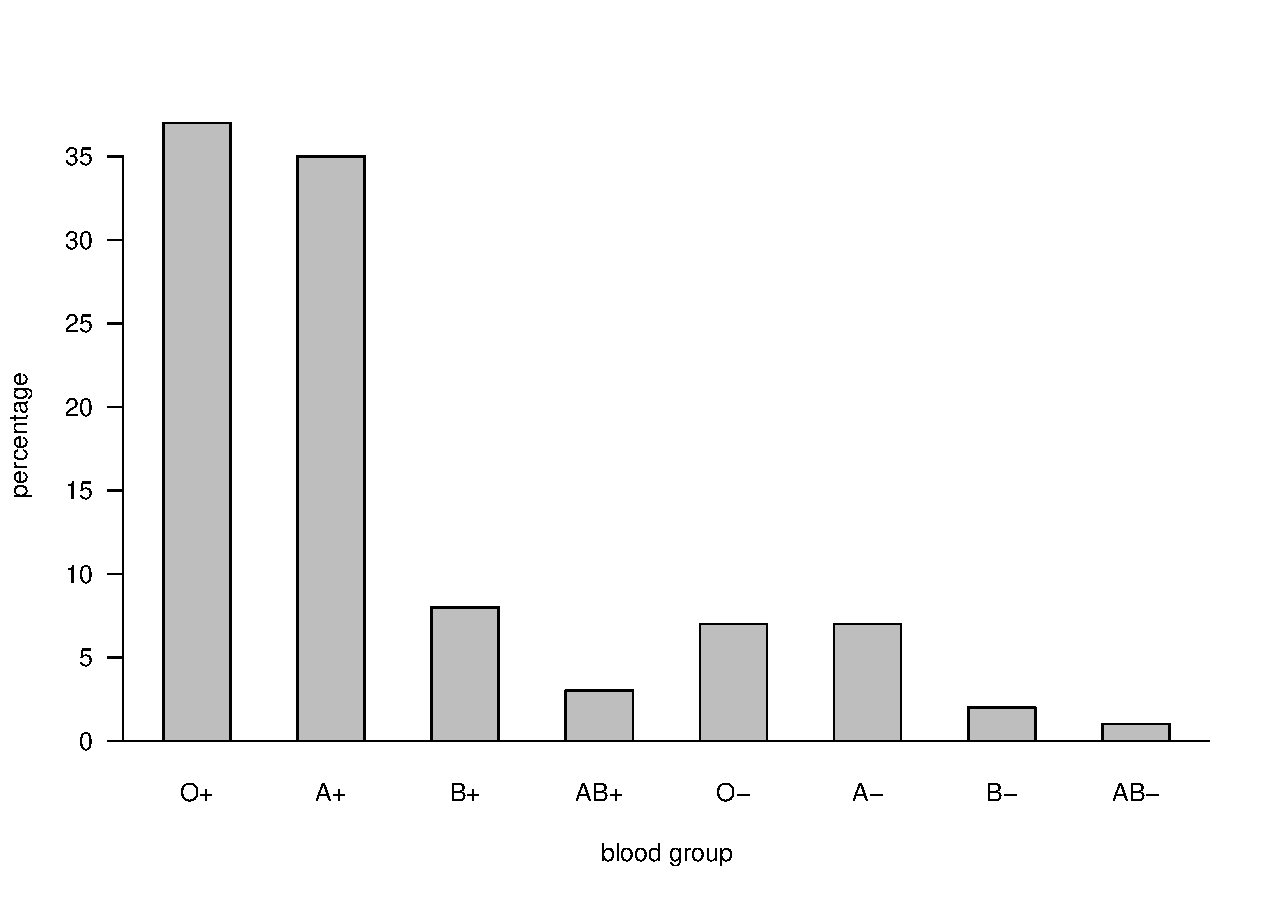
\includegraphics[width=0.6\linewidth]{images/ABO_barplots} 

}

\caption{Barplot of the UK ABO blood group percentages.}\label{fig:ABObar}
\end{figure}

\begin{figure}

{\centering 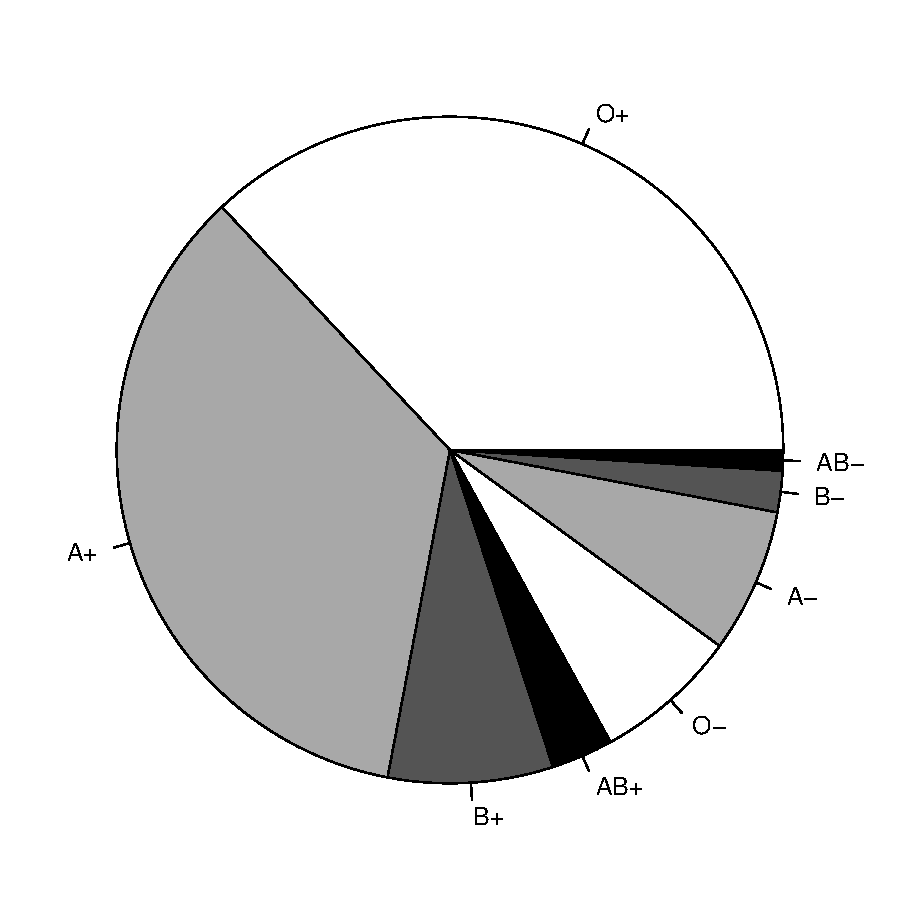
\includegraphics[width=0.75\linewidth]{images/ABO_pie} 

}

\caption{Pie chart (right) of the UK ABO blood group percentages.}\label{fig:ABOpie}
\end{figure}

\hypertarget{times-series-plots}{%
\subsection{Times series plots}\label{times-series-plots}}

The top plot of Figure \ref{fig:ftsenew} shows a \textbf{time series plot} (or time plot) of the weekly closing prices of the FTSE 100 share index from 2nd April 1984 to 13th August 2007. The bottom plot in this figure shows a different version of the same plot.

\begin{figure}

{\centering 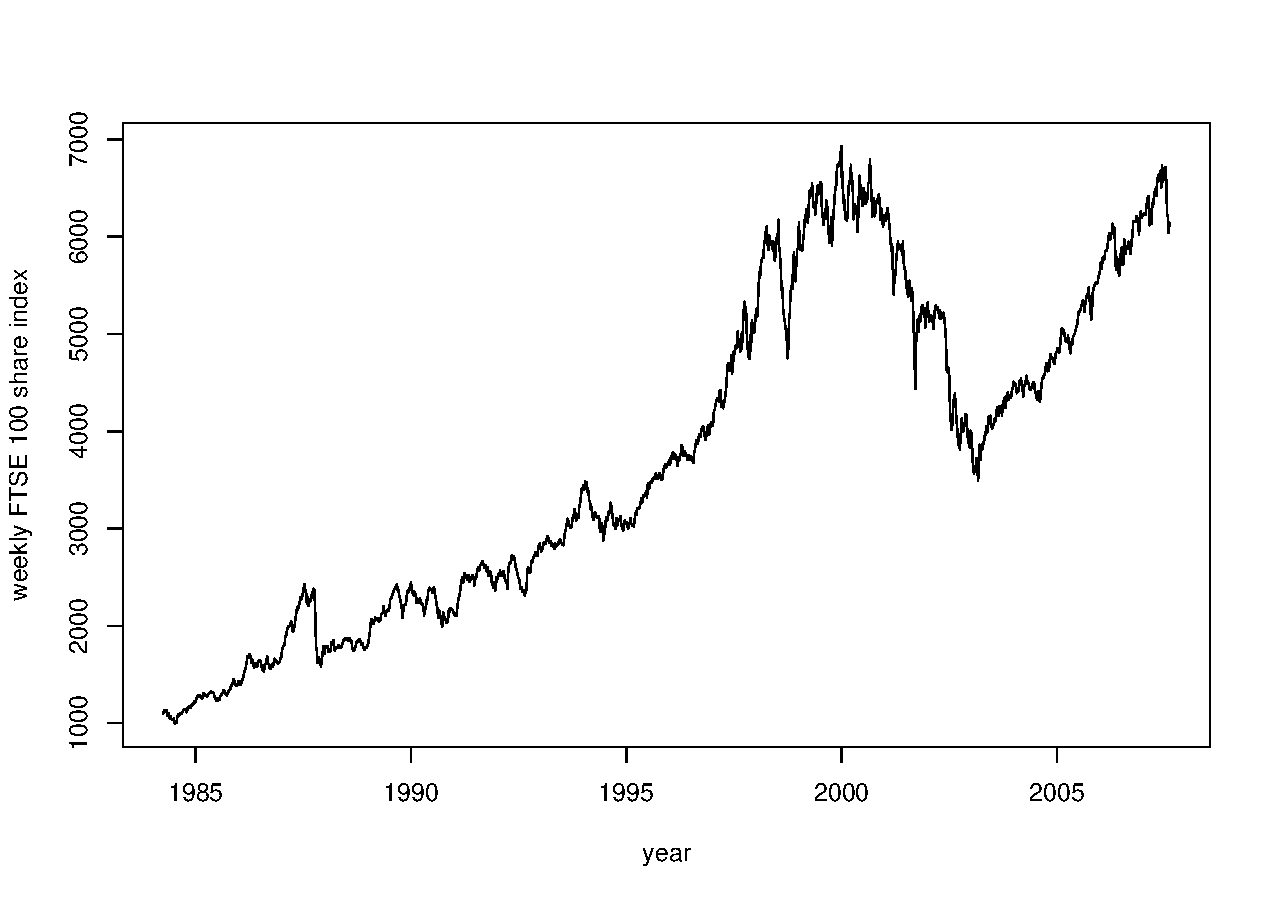
\includegraphics[width=0.75\linewidth]{images/ftse_weekly} 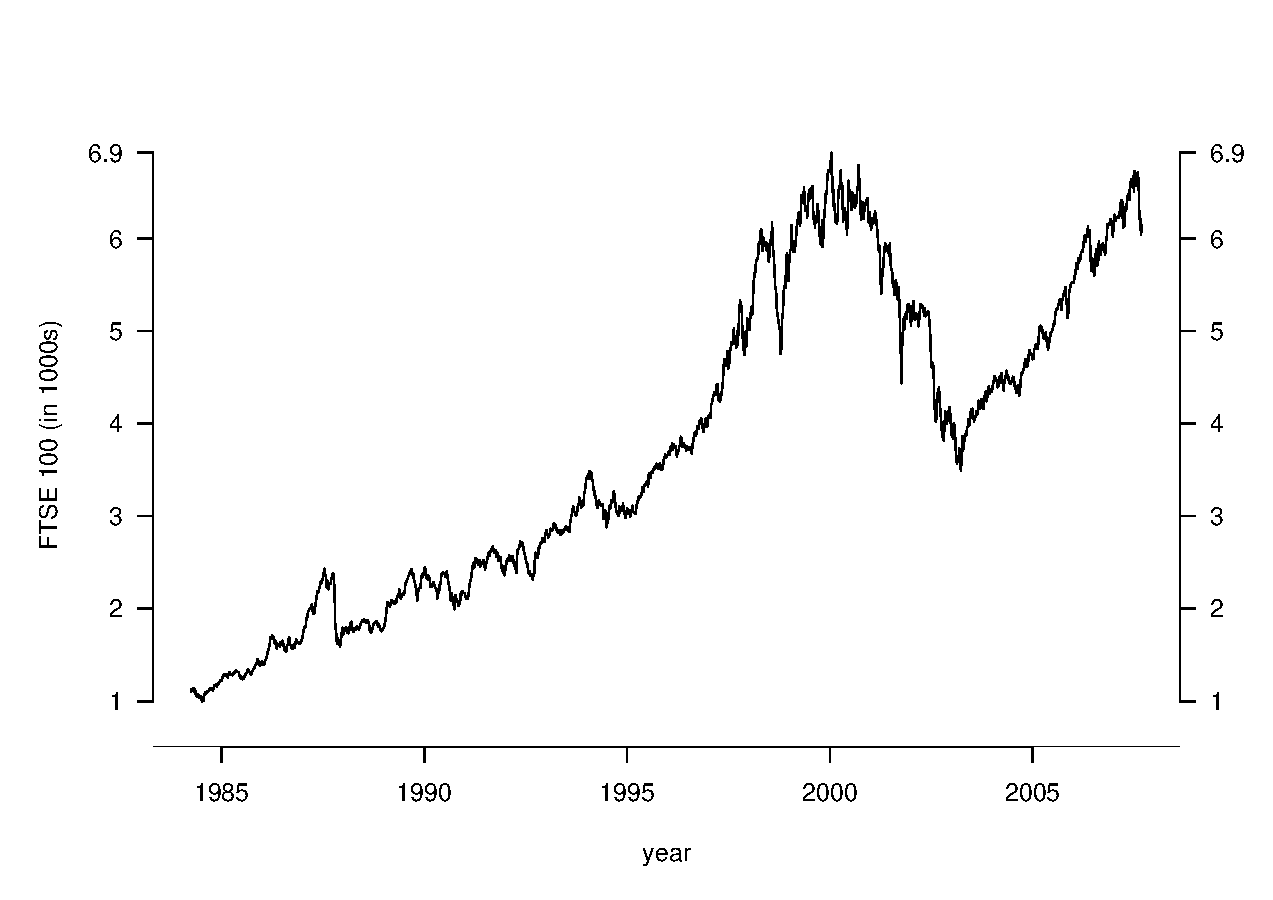
\includegraphics[width=0.75\linewidth]{images/ftse_weekly_tufte} 

}

\caption{Time series plots of the FTSE 100 weekly closing values, 1984--2007.  Top: default plot.  Bottom: modified version, with two vertical axes and the index measured in 1000s.}\label{fig:ftsenew}
\end{figure}

When observations are a time series, that is they are in time order, it is important to plot them against time to look for patterns. The sort of features that often turn up are upward or downward trends, or cyclical behaviour (alternative increases and decreases, often the result of seasonal behaviour),
but you may see other aspects worth noting. Note that

\begin{itemize}
\tightlist
\item
  time should be plotted on the horizontal axis;
\item
  the plot should be wider than it is high;
\item
  joining the dots can help to make interesting patterns easier to see.
\end{itemize}

Figure \ref{fig:fluts} shows a time series plot of another set of data. Can you guess what these data might be?

\begin{figure}

{\centering 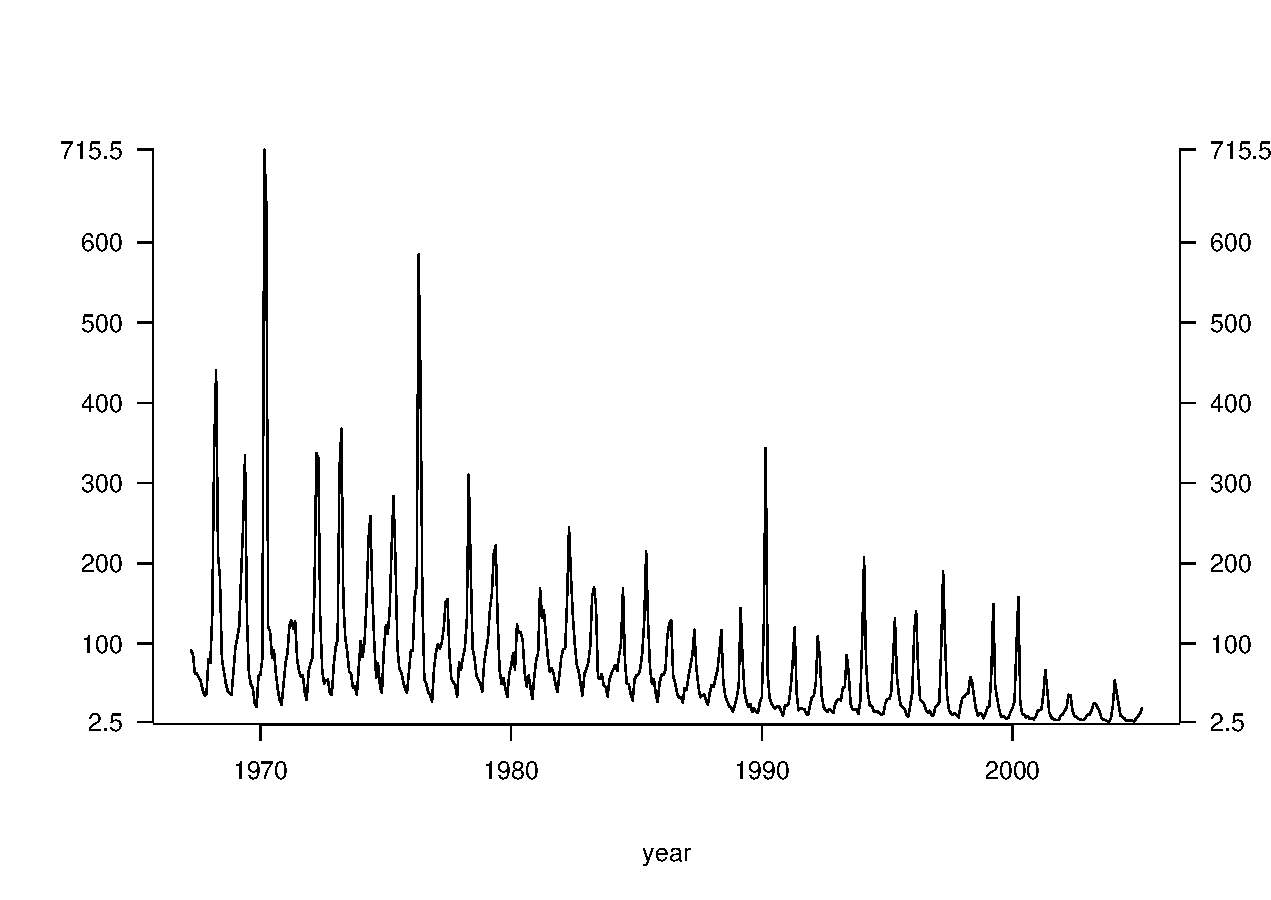
\includegraphics[width=0.75\linewidth]{images/flu_tufte_no_label} 

}

\caption{A time series plot of ?.}\label{fig:fluts}
\end{figure}

\hypertarget{election}{%
\section{2000 US presidential election}\label{election}}

Smith, R. L. (2002) \href{https://doi.org/10.1214/ss/1049993203}{A Statistical Assessment of Buchanan's Vote in Palm Beach County}. \emph{Statistcal Science}, \textbf{17}(4), 441--457.

In the 2000 U.S. Presidential election George W. Bush, the Republican candidate, narrowly beat Al Gore, the Democrat candidate. The result in the state of Florida was particularly close: Al Gore lost by only 537 votes out of 6 million votes cast. If Al Gore had won in Florida he would have become the U.S. President. After the election many allegations of voting irregularities were made and it was a month before Al Gore conceded defeat.

One of the results which caused most surprise was in Palm Beach County, Florida. Pat Buchanan, the Reform Party candidate, got an unexpectedly large 3,407 votes. Based on results in Florida as a whole only 1,300 votes would be expected. Also, given that Palm Beach is largely a Democratic County, a right-wing candidate such as Buchanan would expect even fewer votes.

In the days following the election it was suggested that the type of ballot paper, a so-called Butterfly Ballot \ref{fig:butterfly} used in Palm Beach had confused voters and lead to votes being cast for Buchanan by mistake. People found the Buchanan vote in Palm Beach surprising and there is a plausible explanation for how it occurred.

\begin{figure}

{\centering \includegraphics[width=0.75\linewidth]{images/butterflyballot} 

}

\caption{The Butterfly Ballot used in Palm Beach county.}\label{fig:butterfly}
\end{figure}

\citet{election} uses election results, and other data (on race, age, education and income), from Florida to answer the following questions:

\begin{enumerate}
\def\labelenumi{\arabic{enumi}.}
\tightlist
\item
  Is Buchanan's vote of 3,407 very clearly out of line with the pattern of results form the rest of Florida? In Statistics we call such data values \textbf{outliers}.
\item
  What level of vote for Buchanan would have been realistic in Palm Beach County?
\end{enumerate}

Figure \ref{fig:election1} suggests that the answer to question 1. is ``Yes''.

\begin{figure}

{\centering 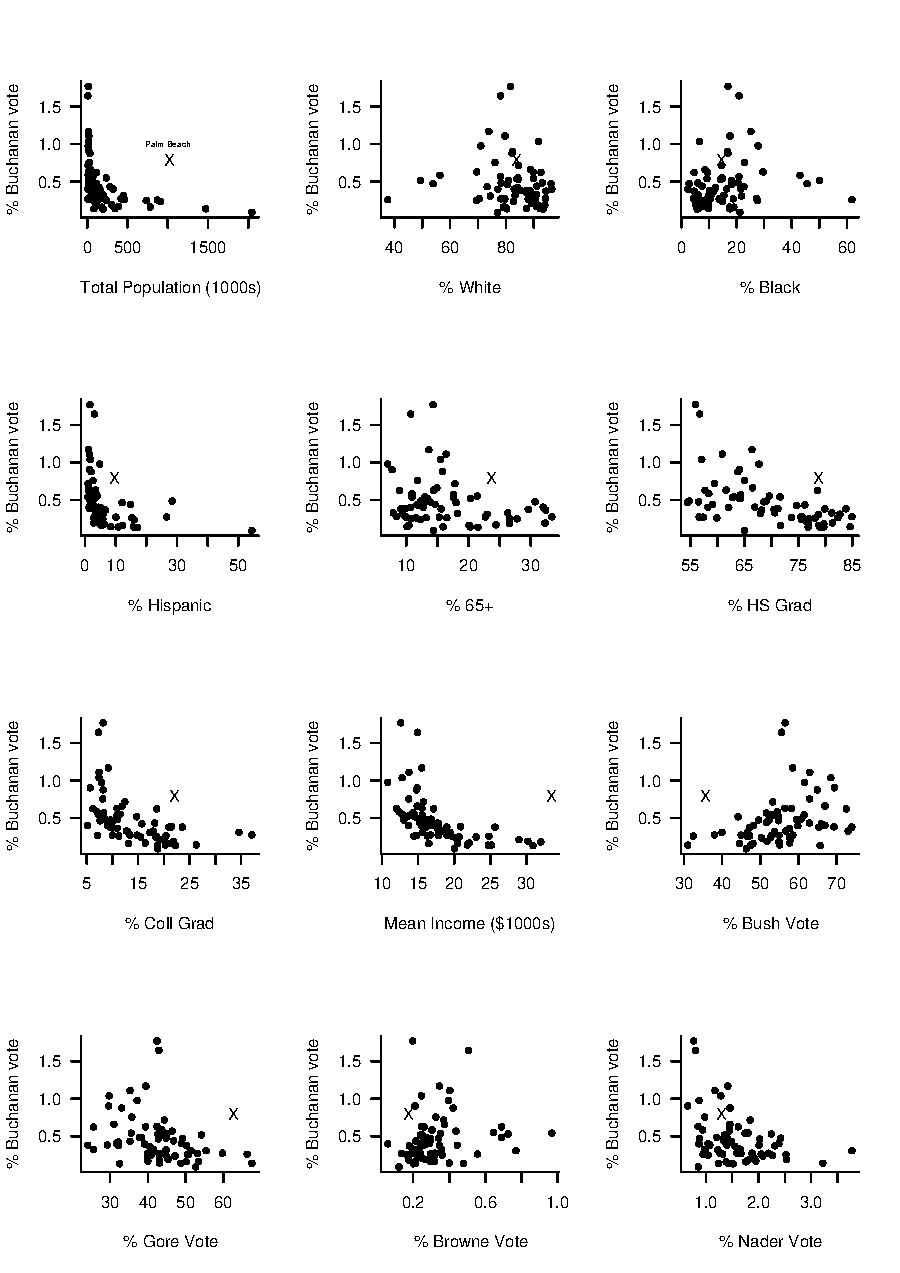
\includegraphics[width=0.75\linewidth]{images/election1} 

}

\caption{ Percentage of Buchanan votes against explanatory variables.  Palm Beach County is marked with a cross.}\label{fig:election1}
\end{figure}

On several of these plots Palm Beach stands out as a clear outlier. In these cases Buchanan gets many more votes than the pattern of the other points would suggest. We also see that the percentage of the vote that Buchanan gets tends to

\begin{itemize}
\tightlist
\item
  decrease with population size;
\item
  decrease with the percentage of of Hispanics;
\item
  decrease with the percentage of voters aged 65 or over;
\item
  decrease with high school and college graduation rate;
\item
  decrease with mean personal income;
\item
  decrease with the percentage of Gore votes;
\item
  increase with the percentage of Bush votes.
\end{itemize}

\citet{election} answers questions 1. and 2. more formally by building a linear regression model. This model quantifies how the percentage of Buchanan vote \(Y\), the \textbf{response variable}, depends on the other variables,the \textbf{explanatory variables} \(x_1,\ldots,x_{12}\). The general idea is to

\begin{itemize}
\tightlist
\item
  build the model using all the data for Florida, apart from the data from Palm Beach, using only the explanatory variables that have a significant effect;
\item
  predict the value of the Buchanan's vote in Palm Beach using the model.
\end{itemize}

We will study simple linear regression models (with only one explanatory variable) towards the end of STAT0002 (Chapter \ref{linreg}) and in STAT0003. The basic idea is to assume that a response variable has a linear (straight line) relationship with explanatory variables. The relationship will not be exact, so the model includes a \textbf{random error} term.

\citet{election} finds that transformations are required in order that the assumptions of the model are satisfied approximately. In particular he finds that using the response variable \(\sqrt{Y}\) is better than using \(Y\) itself (and better than other possible transformations). He also uses a \(\log_{10}\) transformation on some of the explanatory variables (for example Total Population), that is, he uses \(\log_{10}(x)\) rather than \(x\). Figure \ref{fig:election2} is a new version of figure \ref{fig:election1} in which the square root of the percentage of the vote obtained by Buchanan is plotted against the (possibly log-transformed) explanatory variables.

\citet{election} uses transformations of the original data in order to satisfy more closely the assumptions of the linear regression model:

\begin{itemize}
\tightlist
\item
  response = \(\sqrt{Y}\), instead of \(Y\);
\item
  for some explanatory variables, use \(\log_{10}(x)\) instead of \(x\).
\end{itemize}

\begin{figure}

{\centering 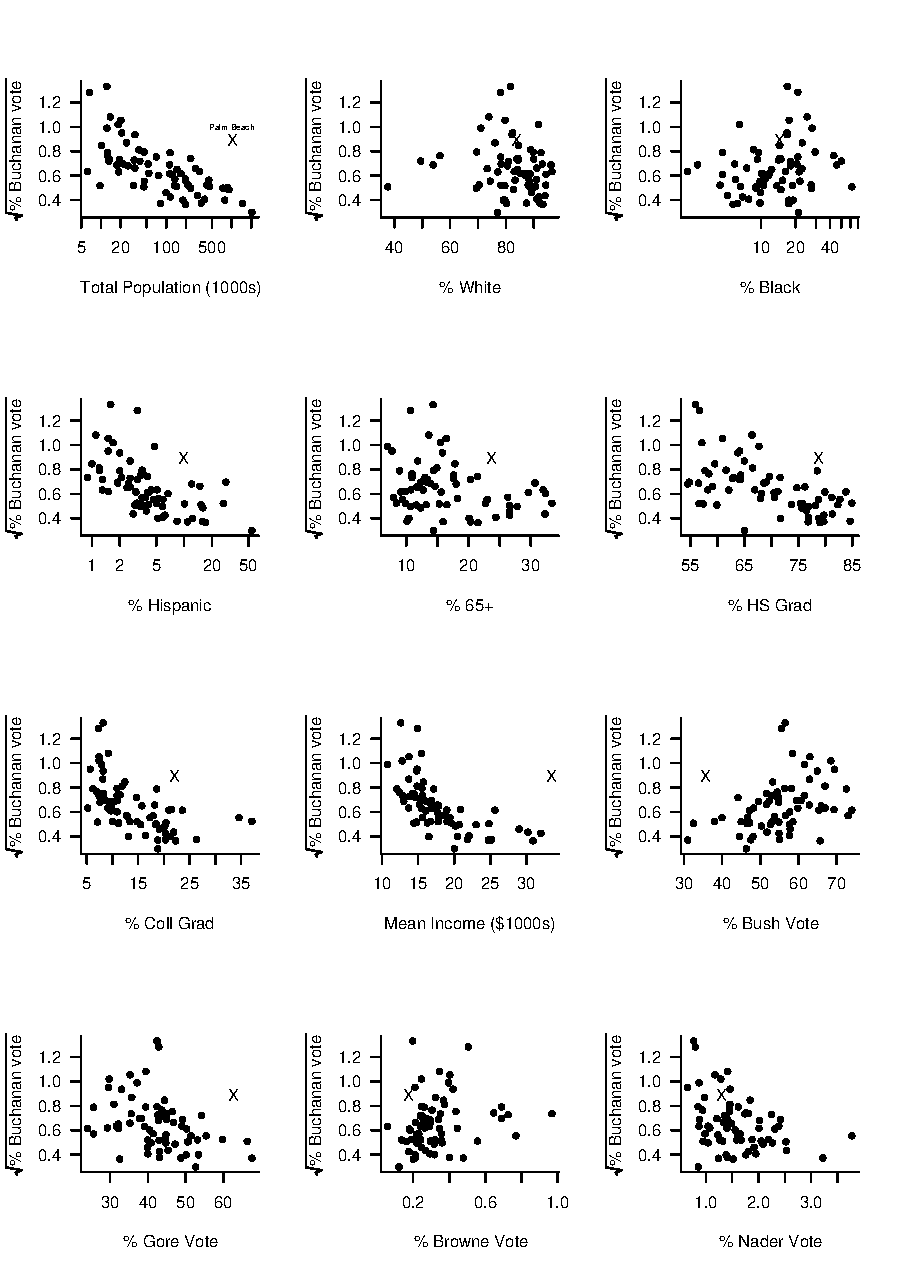
\includegraphics[width=0.75\linewidth]{images/election2} 

}

\caption{The square root of the percentage of Buchanan votes against explanatory variables.  Palm Beach County is marked with a cross.  Note the log scale on the $x$-axis of some plots.}\label{fig:election2}
\end{figure}

\hypertarget{log-scales-on-axes}{%
\subsubsection*{Log scales on axes}\label{log-scales-on-axes}}
\addcontentsline{toc}{subsubsection}{Log scales on axes}

Suppose that we produce a scatter plot where the data on the \(x\)-axis are 0.1, 1, 10, 100 and 1000. If we wish to plot \(\log_{10}(x)\) on the axis instead of \(x\) we have two choices:

\begin{enumerate}
\def\labelenumi{(\alph{enumi})}
\tightlist
\item
  Calculate \(\log_{10}(x)\) and plot these values on the axis.
\item
  Plot the values of \(x\) but on a \(\log_{10}\) scale. On a \(\log_{10}\) scale the values 0.1, 1, 10, 100 and 1000 are equally spaced. For example, from the basic rules of logs we have
  \[\log_{10}(10r) = \log_{10}(10)+\log_{10}(r)=1+\log_{10}(r).\]
  Therefore, on a \(\log_{10}\) scale the values \(10r\) and \(r\) are 1 unit apart. In other words adding 1 unit on a \(\log_{10}(x)\) scale corresponds to \textbf{multiplying} by 10 on the original \(x\)-scale.
\end{enumerate}

Both a. and b. will give exactly the same pattern of plot. The advantage of b. is that the original values are on the plot rather than the \(\log_{10}(x)\)
values. Figure \ref{fig:logaxes} illustrates this.

\begin{figure}

{\centering \includegraphics[width=0.75\linewidth]{images/log_axes} 

}

\caption{Plots to illustrate log-transformation of axes. Top: values of $x$ plotted. Middle: values of $\log_{10}(x)$ plotted. Bottom: values of $x$ plotted on a log-scale.}\label{fig:logaxes}
\end{figure}

Other notes on logs:

\begin{itemize}
\tightlist
\item
  we have used logs to base 10 for simplicity but the base doesn't matter;
\item
  logs are often helpful when the raw data are ratios (e.g.~\(x/y\)) or products (e.g.~\(xy\)). For example, exchange rates and price indices are ratios. If \(x=y\) then \(\log (x/y)=0\); if \(x=k\,y\) then \(\log (x/y)=\log k\); if \(y=k\,x\) then \(\log (x/y)=\log(1/k)=-\log k\); which is a nice symmetry.
\end{itemize}

Imagine that the model has only one explanatory variable, Total Population. You can imagine fitting this linear regression model as drawing a line of best fit through the points on the graph in the top left hand corner of figure \ref{fig:election2}. With more than one explanatory variable it is more complicated than this but the basic idea is the same.

After removing the Buchanan vote in Palm Beach (which we have decided is an outlier) \citet{election} finds that the model fits the data well.

The model predicts the Buchanan vote in Palm Beach to be 371, much lower than the official result of 3,407. This number (371) represents the `best guess' at the Buchanan vote given the other data. To show just how unlikely was the vote of 3,407, \citet{election} calculates a 95\% prediction interval of (219,534) for the Buchanan vote at Palm Beach. If the model is true, this interval has a probability of 95\% of containing the true value of the Buchanan vote.

Smith's analysis suggests that the true Buchanan vote should be approximately 3,000 votes lower than the official result. Given the design of the Butterfly Ballot it seems likely that most of these votes were intended for Al Gore. This would have given Gore the presidency instead of Bush.

\hypertarget{graphs2}{%
\section{Graphs (2 variables)}\label{graphs2}}

When we have 2 continuous variables it is common to examine the relationship between them using a \textbf{scatter plot}.

\hypertarget{scatter-plots}{%
\subsection{Scatter plots}\label{scatter-plots}}

We have already seen some scatter plots in the 2000 US Presidential Election example. We reproduce two of these plots in Figures \ref{fig:scatter1a} and \ref{fig:scatter1b}. A scatter plot is used to examine the relationship between two variables. We need the data to occur in pairs. In Figures \ref{fig:scatter1a} and \ref{fig:scatter1b} each county has a pair of observations: the percentage of votes for Buchanan and the value of the explanatory variable.

\begin{figure}

{\centering 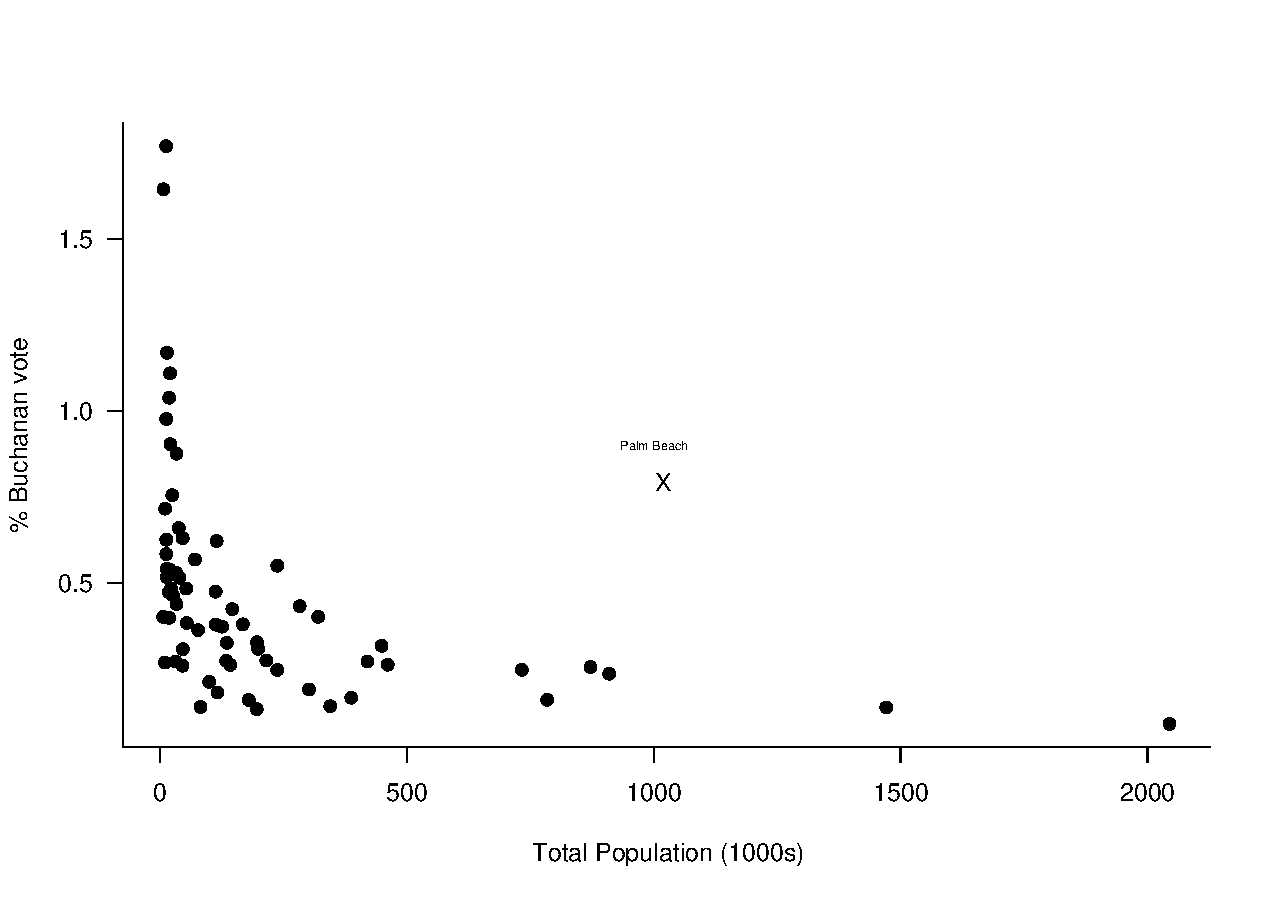
\includegraphics[width=0.75\linewidth]{images/election_scatter1a} 

}

\caption{Scatter plot of the percentage of the vote obtained by Buchanan against the total population from the 2000 US Presidential Election data.}\label{fig:scatter1a}
\end{figure}

\begin{figure}

{\centering 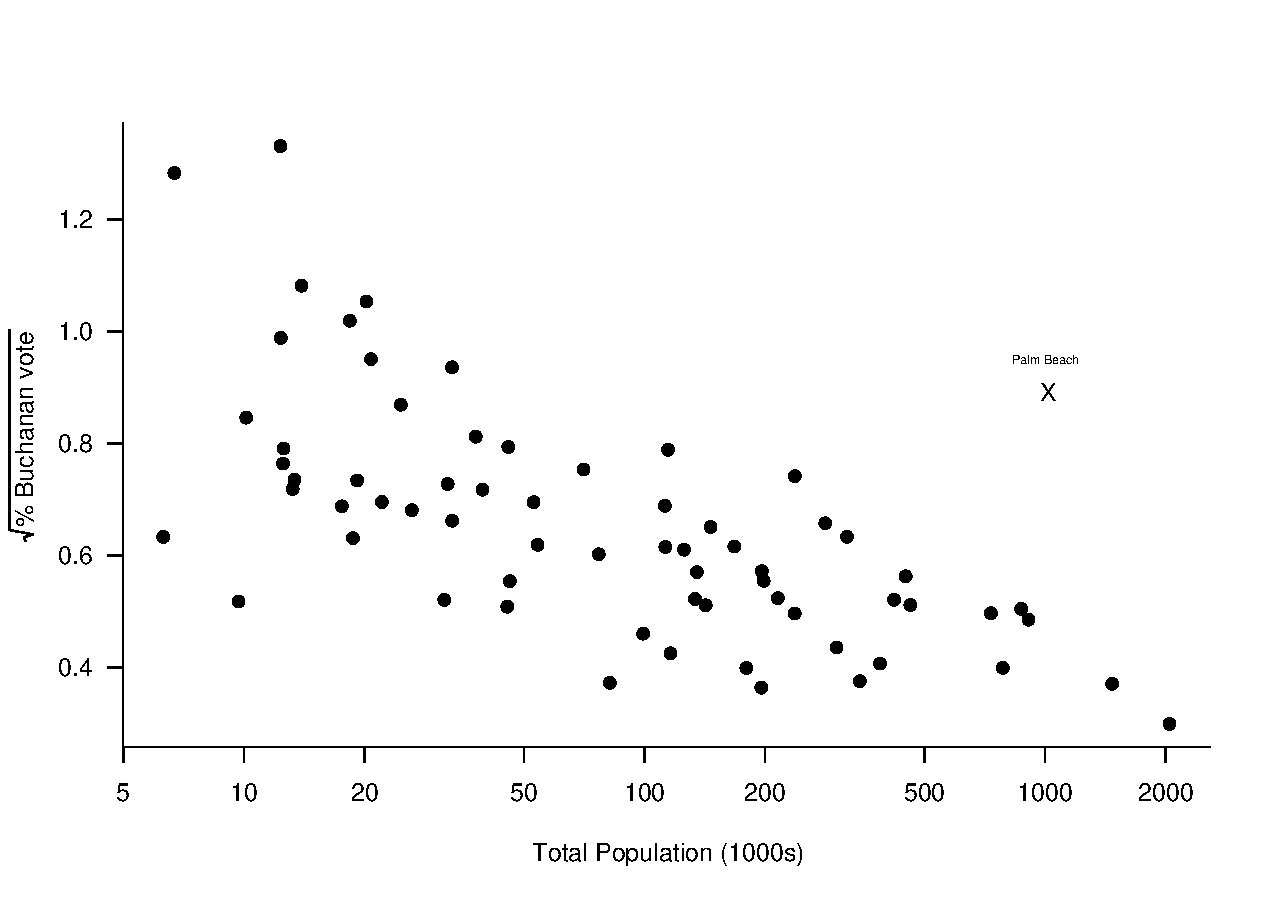
\includegraphics[width=0.75\linewidth]{images/election_scatter1b} 

}

\caption{Scatter plot of the square root of the percentage of the vote obtained by Buchanan against the log of the total population from the 2000 US Presidential Election data.  The plot suggests that these variables are aproximately linearly related.}\label{fig:scatter1b}
\end{figure}

Notice that we have plotted \% Buchanan vote (on the vertical \(y\)-axis) against total population (on the horizontal \(x\)-axis). This is because it makes sense that \% Buchanan vote depends on total population, that is, the size of population influences the vote, not the other way round.

Rules for deciding which variable to plot on the \(y\)-axis and which on the \(x\)-axis are:

\begin{itemize}
\tightlist
\item
  If the direction of dependence is clear, so that variable \(Y\) depends on variable \(X\). For example, \(X\)=river depth influencing \(Y\)=flow rate.
\item
  If one variable, \(X\), is fixed by an experimenter and then the value of another variable, \(Y\) is observed. For example, \(X\)=dosage of drug and \(Y\)=reduction in blood pressure.
\item
  If we wish to predict one variable, \(Y\), using another, \(X\). For example,
  \(X\)=share value today and \(Y\)=share value tomorrow.
\end{itemize}

It is clear in both these plots that the vote in Palm Beach is an outlier.
However, if we had produced separate plots of \% Buchanan vote and total
population Palm Beach would not appear as an outlier.

\hypertarget{transformation}{%
\section{Transformation of data}\label{transformation}}

Some simple statistical methods are based on assumptions about the statistical properties of the data to which they are applied. For example, there are methods that work well provided that a variable of interest is approximately symmetrically distributed. If a variable has a distribution that is strongly skewed then the method will not have the properties that are expected and the results may be misleading. In linear regression (see Chapter \ref{linreg}) the mean of one variable is represented as being related linearly to the value of another variable. If the reality is that this relationship is far from being linear then results may be very misleading.

If we wish to make use of simple assumptions like symmetry of distribution and/or linearity of relationship, but it is clear that the raw data do not support these assumption, then a legitimate approach is to consider whether the assumptions are satisfied better after we transform the data. We illustrate this idea in Sections \ref{transsymmetry} and \ref{straighten}.

\hypertarget{transsymmetry}{%
\subsection{Transformation to approximate symmetry}\label{transsymmetry}}

The data in Table \ref{tab:clouds} resulted from an experiment (\citet{clouds}) to see whether spraying silver nitrate into a cloud (known as \textbf{seeding} the cloud)
could make it produce more rainfall. 52 clouds were studied. 26 of the clouds were chosen at random and seeded with silver nitrate. The amounts of rainfall, in acre-feet, produced by each cloud is recorded. (An acre-foot is a unit of volume equal to 43,560 feet\(^3\) or, approximately, 1233.5m\(^3\).)

 
  \providecommand{\huxb}[2]{\arrayrulecolor[RGB]{#1}\global\arrayrulewidth=#2pt}
  \providecommand{\huxvb}[2]{\color[RGB]{#1}\vrule width #2pt}
  \providecommand{\huxtpad}[1]{\rule{0pt}{#1}}
  \providecommand{\huxbpad}[1]{\rule[-#1]{0pt}{#1}}

\begin{table}[ht]
\begin{centerbox}
\begin{threeparttable}
\captionsetup{justification=centering,singlelinecheck=off}
\caption{\label{tab:clouds} The rainfall, in acre-feet, from 52 clouds, 26 of which were chosen at random to be seeded with silver nitrate.}
 \setlength{\tabcolsep}{0pt}
\begin{tabularx}{0.75\textwidth}{p{0.1875\textwidth} p{0.1875\textwidth} p{0.1875\textwidth} p{0.1875\textwidth}}


\hhline{>{\huxb{0, 0, 0}{1}}->{\huxb{0, 0, 0}{1}}->{\huxb{0, 0, 0}{1}}->{\huxb{0, 0, 0}{1}}-}
\arrayrulecolor{black}

\multicolumn{2}{!{\huxvb{0, 0, 0}{1}}p{0.375\textwidth+2\tabcolsep}!{\huxvb{0, 0, 0}{4}}!{\huxvb{0, 0, 0}{4}}}{\cellcolor[RGB]{255, 255, 255}\hspace{0pt}\parbox[b]{0.375\textwidth+2\tabcolsep-0pt-6pt}{\huxtpad{0pt + 1em}\centering unseeded\huxbpad{0pt}}} &
\multicolumn{2}{p{0.375\textwidth+2\tabcolsep}!{\huxvb{0, 0, 0}{1}}}{\cellcolor[RGB]{255, 255, 255}\hspace{0pt}\parbox[b]{0.375\textwidth+2\tabcolsep-0pt-6pt}{\huxtpad{0pt + 1em}\centering seeded\huxbpad{0pt}}} \tabularnewline[-0.5pt]


\hhline{>{\huxb{0, 0, 0}{1}}->{\huxb{0, 0, 0}{1}}->{\huxb{0, 0, 0}{1}}->{\huxb{0, 0, 0}{1}}-}
\arrayrulecolor{black}

\multicolumn{1}{!{\huxvb{0, 0, 0}{1}}p{0.1875\textwidth}!{\huxvb{0, 0, 0}{1}}}{\cellcolor[RGB]{255, 255, 255}\hspace{0pt}\parbox[b]{0.1875\textwidth-0pt-35pt}{\huxtpad{0pt + 1em}\raggedleft 1202.6\huxbpad{0pt}}} &
\multicolumn{1}{p{0.1875\textwidth}!{\huxvb{0, 0, 0}{4}}!{\huxvb{0, 0, 0}{4}}}{\cellcolor[RGB]{255, 255, 255}\hspace{0pt}\parbox[b]{0.1875\textwidth-0pt-35pt}{\huxtpad{0pt + 1em}\raggedleft 41.1\huxbpad{0pt}}} &
\multicolumn{1}{p{0.1875\textwidth}!{\huxvb{0, 0, 0}{1}}}{\cellcolor[RGB]{255, 255, 255}\hspace{0pt}\parbox[b]{0.1875\textwidth-0pt-35pt}{\huxtpad{0pt + 1em}\raggedleft 2745.6\huxbpad{0pt}}} &
\multicolumn{1}{p{0.1875\textwidth}!{\huxvb{0, 0, 0}{1}}}{\cellcolor[RGB]{255, 255, 255}\hspace{0pt}\parbox[b]{0.1875\textwidth-0pt-35pt}{\huxtpad{0pt + 1em}\raggedleft 200.7\huxbpad{0pt}}} \tabularnewline[-0.5pt]


\hhline{>{\huxb{255, 255, 255}{0.1}}->{\huxb{255, 255, 255}{0.1}}->{\huxb{255, 255, 255}{0.1}}->{\huxb{255, 255, 255}{0.1}}-}
\arrayrulecolor{black}

\multicolumn{1}{!{\huxvb{0, 0, 0}{1}}p{0.1875\textwidth}!{\huxvb{0, 0, 0}{1}}}{\cellcolor[RGB]{255, 255, 255}\hspace{0pt}\parbox[b]{0.1875\textwidth-0pt-35pt}{\huxtpad{0pt + 1em}\raggedleft 830.1\huxbpad{0pt}}} &
\multicolumn{1}{p{0.1875\textwidth}!{\huxvb{0, 0, 0}{4}}!{\huxvb{0, 0, 0}{4}}}{\cellcolor[RGB]{255, 255, 255}\hspace{0pt}\parbox[b]{0.1875\textwidth-0pt-35pt}{\huxtpad{0pt + 1em}\raggedleft 36.6\huxbpad{0pt}}} &
\multicolumn{1}{p{0.1875\textwidth}!{\huxvb{0, 0, 0}{1}}}{\cellcolor[RGB]{255, 255, 255}\hspace{0pt}\parbox[b]{0.1875\textwidth-0pt-35pt}{\huxtpad{0pt + 1em}\raggedleft 1697.8\huxbpad{0pt}}} &
\multicolumn{1}{p{0.1875\textwidth}!{\huxvb{0, 0, 0}{1}}}{\cellcolor[RGB]{255, 255, 255}\hspace{0pt}\parbox[b]{0.1875\textwidth-0pt-35pt}{\huxtpad{0pt + 1em}\raggedleft 198.6\huxbpad{0pt}}} \tabularnewline[-0.5pt]


\hhline{>{\huxb{255, 255, 255}{0.1}}->{\huxb{255, 255, 255}{0.1}}->{\huxb{255, 255, 255}{0.1}}->{\huxb{255, 255, 255}{0.1}}-}
\arrayrulecolor{black}

\multicolumn{1}{!{\huxvb{0, 0, 0}{1}}p{0.1875\textwidth}!{\huxvb{0, 0, 0}{1}}}{\cellcolor[RGB]{255, 255, 255}\hspace{0pt}\parbox[b]{0.1875\textwidth-0pt-35pt}{\huxtpad{0pt + 1em}\raggedleft 372.4\huxbpad{0pt}}} &
\multicolumn{1}{p{0.1875\textwidth}!{\huxvb{0, 0, 0}{4}}!{\huxvb{0, 0, 0}{4}}}{\cellcolor[RGB]{255, 255, 255}\hspace{0pt}\parbox[b]{0.1875\textwidth-0pt-35pt}{\huxtpad{0pt + 1em}\raggedleft 29.0\huxbpad{0pt}}} &
\multicolumn{1}{p{0.1875\textwidth}!{\huxvb{0, 0, 0}{1}}}{\cellcolor[RGB]{255, 255, 255}\hspace{0pt}\parbox[b]{0.1875\textwidth-0pt-35pt}{\huxtpad{0pt + 1em}\raggedleft 1656.0\huxbpad{0pt}}} &
\multicolumn{1}{p{0.1875\textwidth}!{\huxvb{0, 0, 0}{1}}}{\cellcolor[RGB]{255, 255, 255}\hspace{0pt}\parbox[b]{0.1875\textwidth-0pt-35pt}{\huxtpad{0pt + 1em}\raggedleft 129.6\huxbpad{0pt}}} \tabularnewline[-0.5pt]


\hhline{>{\huxb{255, 255, 255}{0.1}}->{\huxb{255, 255, 255}{0.1}}->{\huxb{255, 255, 255}{0.1}}->{\huxb{255, 255, 255}{0.1}}-}
\arrayrulecolor{black}

\multicolumn{1}{!{\huxvb{0, 0, 0}{1}}p{0.1875\textwidth}!{\huxvb{0, 0, 0}{1}}}{\cellcolor[RGB]{255, 255, 255}\hspace{0pt}\parbox[b]{0.1875\textwidth-0pt-35pt}{\huxtpad{0pt + 1em}\raggedleft 345.5\huxbpad{0pt}}} &
\multicolumn{1}{p{0.1875\textwidth}!{\huxvb{0, 0, 0}{4}}!{\huxvb{0, 0, 0}{4}}}{\cellcolor[RGB]{255, 255, 255}\hspace{0pt}\parbox[b]{0.1875\textwidth-0pt-35pt}{\huxtpad{0pt + 1em}\raggedleft 28.6\huxbpad{0pt}}} &
\multicolumn{1}{p{0.1875\textwidth}!{\huxvb{0, 0, 0}{1}}}{\cellcolor[RGB]{255, 255, 255}\hspace{0pt}\parbox[b]{0.1875\textwidth-0pt-35pt}{\huxtpad{0pt + 1em}\raggedleft 978.0\huxbpad{0pt}}} &
\multicolumn{1}{p{0.1875\textwidth}!{\huxvb{0, 0, 0}{1}}}{\cellcolor[RGB]{255, 255, 255}\hspace{0pt}\parbox[b]{0.1875\textwidth-0pt-35pt}{\huxtpad{0pt + 1em}\raggedleft 119.0\huxbpad{0pt}}} \tabularnewline[-0.5pt]


\hhline{>{\huxb{255, 255, 255}{0.1}}->{\huxb{255, 255, 255}{0.1}}->{\huxb{255, 255, 255}{0.1}}->{\huxb{255, 255, 255}{0.1}}-}
\arrayrulecolor{black}

\multicolumn{1}{!{\huxvb{0, 0, 0}{1}}p{0.1875\textwidth}!{\huxvb{0, 0, 0}{1}}}{\cellcolor[RGB]{255, 255, 255}\hspace{0pt}\parbox[b]{0.1875\textwidth-0pt-35pt}{\huxtpad{0pt + 1em}\raggedleft 321.2\huxbpad{0pt}}} &
\multicolumn{1}{p{0.1875\textwidth}!{\huxvb{0, 0, 0}{4}}!{\huxvb{0, 0, 0}{4}}}{\cellcolor[RGB]{255, 255, 255}\hspace{0pt}\parbox[b]{0.1875\textwidth-0pt-35pt}{\huxtpad{0pt + 1em}\raggedleft 26.3\huxbpad{0pt}}} &
\multicolumn{1}{p{0.1875\textwidth}!{\huxvb{0, 0, 0}{1}}}{\cellcolor[RGB]{255, 255, 255}\hspace{0pt}\parbox[b]{0.1875\textwidth-0pt-35pt}{\huxtpad{0pt + 1em}\raggedleft 703.4\huxbpad{0pt}}} &
\multicolumn{1}{p{0.1875\textwidth}!{\huxvb{0, 0, 0}{1}}}{\cellcolor[RGB]{255, 255, 255}\hspace{0pt}\parbox[b]{0.1875\textwidth-0pt-35pt}{\huxtpad{0pt + 1em}\raggedleft 118.3\huxbpad{0pt}}} \tabularnewline[-0.5pt]


\hhline{>{\huxb{255, 255, 255}{0.1}}->{\huxb{255, 255, 255}{0.1}}->{\huxb{255, 255, 255}{0.1}}->{\huxb{255, 255, 255}{0.1}}-}
\arrayrulecolor{black}

\multicolumn{1}{!{\huxvb{0, 0, 0}{1}}p{0.1875\textwidth}!{\huxvb{0, 0, 0}{1}}}{\cellcolor[RGB]{255, 255, 255}\hspace{0pt}\parbox[b]{0.1875\textwidth-0pt-35pt}{\huxtpad{0pt + 1em}\raggedleft 244.3\huxbpad{0pt}}} &
\multicolumn{1}{p{0.1875\textwidth}!{\huxvb{0, 0, 0}{4}}!{\huxvb{0, 0, 0}{4}}}{\cellcolor[RGB]{255, 255, 255}\hspace{0pt}\parbox[b]{0.1875\textwidth-0pt-35pt}{\huxtpad{0pt + 1em}\raggedleft 26.1\huxbpad{0pt}}} &
\multicolumn{1}{p{0.1875\textwidth}!{\huxvb{0, 0, 0}{1}}}{\cellcolor[RGB]{255, 255, 255}\hspace{0pt}\parbox[b]{0.1875\textwidth-0pt-35pt}{\huxtpad{0pt + 1em}\raggedleft 489.1\huxbpad{0pt}}} &
\multicolumn{1}{p{0.1875\textwidth}!{\huxvb{0, 0, 0}{1}}}{\cellcolor[RGB]{255, 255, 255}\hspace{0pt}\parbox[b]{0.1875\textwidth-0pt-35pt}{\huxtpad{0pt + 1em}\raggedleft 115.3\huxbpad{0pt}}} \tabularnewline[-0.5pt]


\hhline{>{\huxb{255, 255, 255}{0.1}}->{\huxb{255, 255, 255}{0.1}}->{\huxb{255, 255, 255}{0.1}}->{\huxb{255, 255, 255}{0.1}}-}
\arrayrulecolor{black}

\multicolumn{1}{!{\huxvb{0, 0, 0}{1}}p{0.1875\textwidth}!{\huxvb{0, 0, 0}{1}}}{\cellcolor[RGB]{255, 255, 255}\hspace{0pt}\parbox[b]{0.1875\textwidth-0pt-35pt}{\huxtpad{0pt + 1em}\raggedleft 163.0\huxbpad{0pt}}} &
\multicolumn{1}{p{0.1875\textwidth}!{\huxvb{0, 0, 0}{4}}!{\huxvb{0, 0, 0}{4}}}{\cellcolor[RGB]{255, 255, 255}\hspace{0pt}\parbox[b]{0.1875\textwidth-0pt-35pt}{\huxtpad{0pt + 1em}\raggedleft 24.4\huxbpad{0pt}}} &
\multicolumn{1}{p{0.1875\textwidth}!{\huxvb{0, 0, 0}{1}}}{\cellcolor[RGB]{255, 255, 255}\hspace{0pt}\parbox[b]{0.1875\textwidth-0pt-35pt}{\huxtpad{0pt + 1em}\raggedleft 430.0\huxbpad{0pt}}} &
\multicolumn{1}{p{0.1875\textwidth}!{\huxvb{0, 0, 0}{1}}}{\cellcolor[RGB]{255, 255, 255}\hspace{0pt}\parbox[b]{0.1875\textwidth-0pt-35pt}{\huxtpad{0pt + 1em}\raggedleft 92.4\huxbpad{0pt}}} \tabularnewline[-0.5pt]


\hhline{>{\huxb{255, 255, 255}{0.1}}->{\huxb{255, 255, 255}{0.1}}->{\huxb{255, 255, 255}{0.1}}->{\huxb{255, 255, 255}{0.1}}-}
\arrayrulecolor{black}

\multicolumn{1}{!{\huxvb{0, 0, 0}{1}}p{0.1875\textwidth}!{\huxvb{0, 0, 0}{1}}}{\cellcolor[RGB]{255, 255, 255}\hspace{0pt}\parbox[b]{0.1875\textwidth-0pt-35pt}{\huxtpad{0pt + 1em}\raggedleft 147.8\huxbpad{0pt}}} &
\multicolumn{1}{p{0.1875\textwidth}!{\huxvb{0, 0, 0}{4}}!{\huxvb{0, 0, 0}{4}}}{\cellcolor[RGB]{255, 255, 255}\hspace{0pt}\parbox[b]{0.1875\textwidth-0pt-35pt}{\huxtpad{0pt + 1em}\raggedleft 21.7\huxbpad{0pt}}} &
\multicolumn{1}{p{0.1875\textwidth}!{\huxvb{0, 0, 0}{1}}}{\cellcolor[RGB]{255, 255, 255}\hspace{0pt}\parbox[b]{0.1875\textwidth-0pt-35pt}{\huxtpad{0pt + 1em}\raggedleft 334.1\huxbpad{0pt}}} &
\multicolumn{1}{p{0.1875\textwidth}!{\huxvb{0, 0, 0}{1}}}{\cellcolor[RGB]{255, 255, 255}\hspace{0pt}\parbox[b]{0.1875\textwidth-0pt-35pt}{\huxtpad{0pt + 1em}\raggedleft 40.6\huxbpad{0pt}}} \tabularnewline[-0.5pt]


\hhline{>{\huxb{255, 255, 255}{0.1}}->{\huxb{255, 255, 255}{0.1}}->{\huxb{255, 255, 255}{0.1}}->{\huxb{255, 255, 255}{0.1}}-}
\arrayrulecolor{black}

\multicolumn{1}{!{\huxvb{0, 0, 0}{1}}p{0.1875\textwidth}!{\huxvb{0, 0, 0}{1}}}{\cellcolor[RGB]{255, 255, 255}\hspace{0pt}\parbox[b]{0.1875\textwidth-0pt-35pt}{\huxtpad{0pt + 1em}\raggedleft 95.0\huxbpad{0pt}}} &
\multicolumn{1}{p{0.1875\textwidth}!{\huxvb{0, 0, 0}{4}}!{\huxvb{0, 0, 0}{4}}}{\cellcolor[RGB]{255, 255, 255}\hspace{0pt}\parbox[b]{0.1875\textwidth-0pt-35pt}{\huxtpad{0pt + 1em}\raggedleft 17.3\huxbpad{0pt}}} &
\multicolumn{1}{p{0.1875\textwidth}!{\huxvb{0, 0, 0}{1}}}{\cellcolor[RGB]{255, 255, 255}\hspace{0pt}\parbox[b]{0.1875\textwidth-0pt-35pt}{\huxtpad{0pt + 1em}\raggedleft 302.8\huxbpad{0pt}}} &
\multicolumn{1}{p{0.1875\textwidth}!{\huxvb{0, 0, 0}{1}}}{\cellcolor[RGB]{255, 255, 255}\hspace{0pt}\parbox[b]{0.1875\textwidth-0pt-35pt}{\huxtpad{0pt + 1em}\raggedleft 32.7\huxbpad{0pt}}} \tabularnewline[-0.5pt]


\hhline{>{\huxb{255, 255, 255}{0.1}}->{\huxb{255, 255, 255}{0.1}}->{\huxb{255, 255, 255}{0.1}}->{\huxb{255, 255, 255}{0.1}}-}
\arrayrulecolor{black}

\multicolumn{1}{!{\huxvb{0, 0, 0}{1}}p{0.1875\textwidth}!{\huxvb{0, 0, 0}{1}}}{\cellcolor[RGB]{255, 255, 255}\hspace{0pt}\parbox[b]{0.1875\textwidth-0pt-35pt}{\huxtpad{0pt + 1em}\raggedleft 87.0\huxbpad{0pt}}} &
\multicolumn{1}{p{0.1875\textwidth}!{\huxvb{0, 0, 0}{4}}!{\huxvb{0, 0, 0}{4}}}{\cellcolor[RGB]{255, 255, 255}\hspace{0pt}\parbox[b]{0.1875\textwidth-0pt-35pt}{\huxtpad{0pt + 1em}\raggedleft 11.5\huxbpad{0pt}}} &
\multicolumn{1}{p{0.1875\textwidth}!{\huxvb{0, 0, 0}{1}}}{\cellcolor[RGB]{255, 255, 255}\hspace{0pt}\parbox[b]{0.1875\textwidth-0pt-35pt}{\huxtpad{0pt + 1em}\raggedleft 274.7\huxbpad{0pt}}} &
\multicolumn{1}{p{0.1875\textwidth}!{\huxvb{0, 0, 0}{1}}}{\cellcolor[RGB]{255, 255, 255}\hspace{0pt}\parbox[b]{0.1875\textwidth-0pt-35pt}{\huxtpad{0pt + 1em}\raggedleft 31.4\huxbpad{0pt}}} \tabularnewline[-0.5pt]


\hhline{>{\huxb{255, 255, 255}{0.1}}->{\huxb{255, 255, 255}{0.1}}->{\huxb{255, 255, 255}{0.1}}->{\huxb{255, 255, 255}{0.1}}-}
\arrayrulecolor{black}

\multicolumn{1}{!{\huxvb{0, 0, 0}{1}}p{0.1875\textwidth}!{\huxvb{0, 0, 0}{1}}}{\cellcolor[RGB]{255, 255, 255}\hspace{0pt}\parbox[b]{0.1875\textwidth-0pt-35pt}{\huxtpad{0pt + 1em}\raggedleft 81.2\huxbpad{0pt}}} &
\multicolumn{1}{p{0.1875\textwidth}!{\huxvb{0, 0, 0}{4}}!{\huxvb{0, 0, 0}{4}}}{\cellcolor[RGB]{255, 255, 255}\hspace{0pt}\parbox[b]{0.1875\textwidth-0pt-35pt}{\huxtpad{0pt + 1em}\raggedleft 4.9\huxbpad{0pt}}} &
\multicolumn{1}{p{0.1875\textwidth}!{\huxvb{0, 0, 0}{1}}}{\cellcolor[RGB]{255, 255, 255}\hspace{0pt}\parbox[b]{0.1875\textwidth-0pt-35pt}{\huxtpad{0pt + 1em}\raggedleft 274.7\huxbpad{0pt}}} &
\multicolumn{1}{p{0.1875\textwidth}!{\huxvb{0, 0, 0}{1}}}{\cellcolor[RGB]{255, 255, 255}\hspace{0pt}\parbox[b]{0.1875\textwidth-0pt-35pt}{\huxtpad{0pt + 1em}\raggedleft 17.5\huxbpad{0pt}}} \tabularnewline[-0.5pt]


\hhline{>{\huxb{255, 255, 255}{0.1}}->{\huxb{255, 255, 255}{0.1}}->{\huxb{255, 255, 255}{0.1}}->{\huxb{255, 255, 255}{0.1}}-}
\arrayrulecolor{black}

\multicolumn{1}{!{\huxvb{0, 0, 0}{1}}p{0.1875\textwidth}!{\huxvb{0, 0, 0}{1}}}{\cellcolor[RGB]{255, 255, 255}\hspace{0pt}\parbox[b]{0.1875\textwidth-0pt-35pt}{\huxtpad{0pt + 1em}\raggedleft 68.5\huxbpad{0pt}}} &
\multicolumn{1}{p{0.1875\textwidth}!{\huxvb{0, 0, 0}{4}}!{\huxvb{0, 0, 0}{4}}}{\cellcolor[RGB]{255, 255, 255}\hspace{0pt}\parbox[b]{0.1875\textwidth-0pt-35pt}{\huxtpad{0pt + 1em}\raggedleft 4.9\huxbpad{0pt}}} &
\multicolumn{1}{p{0.1875\textwidth}!{\huxvb{0, 0, 0}{1}}}{\cellcolor[RGB]{255, 255, 255}\hspace{0pt}\parbox[b]{0.1875\textwidth-0pt-35pt}{\huxtpad{0pt + 1em}\raggedleft 255.0\huxbpad{0pt}}} &
\multicolumn{1}{p{0.1875\textwidth}!{\huxvb{0, 0, 0}{1}}}{\cellcolor[RGB]{255, 255, 255}\hspace{0pt}\parbox[b]{0.1875\textwidth-0pt-35pt}{\huxtpad{0pt + 1em}\raggedleft 7.7\huxbpad{0pt}}} \tabularnewline[-0.5pt]


\hhline{>{\huxb{255, 255, 255}{0.1}}->{\huxb{255, 255, 255}{0.1}}->{\huxb{255, 255, 255}{0.1}}->{\huxb{255, 255, 255}{0.1}}-}
\arrayrulecolor{black}

\multicolumn{1}{!{\huxvb{0, 0, 0}{1}}p{0.1875\textwidth}!{\huxvb{0, 0, 0}{1}}}{\cellcolor[RGB]{255, 255, 255}\hspace{0pt}\parbox[b]{0.1875\textwidth-0pt-35pt}{\huxtpad{0pt + 1em}\raggedleft 47.3\huxbpad{0pt}}} &
\multicolumn{1}{p{0.1875\textwidth}!{\huxvb{0, 0, 0}{4}}!{\huxvb{0, 0, 0}{4}}}{\cellcolor[RGB]{255, 255, 255}\hspace{0pt}\parbox[b]{0.1875\textwidth-0pt-35pt}{\huxtpad{0pt + 1em}\raggedleft 1.0\huxbpad{0pt}}} &
\multicolumn{1}{p{0.1875\textwidth}!{\huxvb{0, 0, 0}{1}}}{\cellcolor[RGB]{255, 255, 255}\hspace{0pt}\parbox[b]{0.1875\textwidth-0pt-35pt}{\huxtpad{0pt + 1em}\raggedleft 242.5\huxbpad{0pt}}} &
\multicolumn{1}{p{0.1875\textwidth}!{\huxvb{0, 0, 0}{1}}}{\cellcolor[RGB]{255, 255, 255}\hspace{0pt}\parbox[b]{0.1875\textwidth-0pt-35pt}{\huxtpad{0pt + 1em}\raggedleft 4.1\huxbpad{0pt}}} \tabularnewline[-0.5pt]


\hhline{>{\huxb{0, 0, 0}{1}}->{\huxb{0, 0, 0}{1}}->{\huxb{0, 0, 0}{1}}->{\huxb{0, 0, 0}{1}}-}
\arrayrulecolor{black}
\end{tabularx}
\end{threeparttable}\par\end{centerbox}

\end{table}
 

Figure \ref{fig:cloudboxlog} shows separate boxplots of the rainfall amounts from seeded and unseeded clouds.

\begin{figure}

{\centering \includegraphics[width=0.75\linewidth]{images/cloud_box} 

}

\caption{Boxplots of rainfall in acre-feet for seeded and unseeded clouds.  Sample means are marked with a cross.}\label{fig:cloudbox}
\end{figure}

It is clear from the shape of these plots that the data are positively skewed. Also, the sample means are much greater than their corresponding sample medians. Measurements of (positive) environmental quantities are often positive skew. In addition, the rainfall values from the seeded clouds have a both higher location and a higher spread than the values from the unseeded clouds. After a log transformation (see \ref{fig:cloudboxlog}), the data are closer to being approximately symmetric. The sample means are closer to their corresponding sample medians. In addition the log transformation makes the variances of the rainfall values in the two groups more nearly equal.

\begin{figure}

{\centering \includegraphics[width=0.75\linewidth]{images/cloud_box_log} 

}

\caption{Boxplots of rainfall in acre-feet for seeded and unseeded clouds after a $\log_{10}$ transformation has been applied.  Sample means are mared with a cross.}\label{fig:cloudboxlog}
\end{figure}

We have used a log transformation make positive skew data more symmetric. Other transformations which can be useful for this purpose are: \(y^c\), where \(c<1\), for example, \(\sqrt{y}\), \(1/y\). These transformations stretch out the lower tail. In contrast, \(y^c\), where \(c>1\), e.g.~\(y^2\), \(y^3\), may be used to transform negative skew data to approximate symmetry. These transformations stretch out the upper tail. It may seem that the log transformation is of an entirely different form to the other transformations, that is, \(y^c\) for some \(c \neq 0\). However, we will see that a log transformation can be obtained by considering the behaviour of the equivalent transformation \((y^c - 1) / c\) as \(c\) approaches zero.

It is possible to transform using \(y^c\) for \textbf{any} real value of \(c\), but it is better to stick to simple powers, such as the ones above, as it is more likely that these will have a sensible interpretation. The further \(c\) is from 1 the more difference the transformation makes.

These rainfall data are positive so there is no problem using a transformation of the form \(y^c\). However, if a dataset contains negative values then there are problems. If \(y<0\) then \(y^c\) can only be calculated in special cases where \(c\) is an integer. We also need to be able to invert the transformation, that is, to infer the value of \(y\) uniquely from the value of \(y^c\). If \(y\) can be both negative and positive then this is only possible in the very special cases where \(c\) is an odd integer. If a dataset contains zeros then we cannot use a log transformation, or \(y^c\) for \(c < 0\). The main point is that we need all the data to be positive in order to use the transformation \(y^c\) (or \((y^c - 1) / c\)). If we wish to transform data with non-positive values it is common to add a suitable constant to all values, to produce positive data, before transformation.

The rainfall data range over several orders of magnitude, that is, from one to well over a thousand. Applying a log transformation is often useful when data range over several orders of magnitude.

\textbf{An aside}. If we particularly like stem-and-leaf plots then we could produce a back-to-back stem-and-leaf plot, as in the plots of the log-transformed rainfall totals in Figure \ref{fig:cloudstem}.

\begin{figure}

{\centering \includegraphics[width=0.75\linewidth]{images/cloud_stem} 

}

\caption{Back to back stem-and-leaf plot of $\log_{10}$(rainfall) for the cloud seeding data. The decimal point is at the vertical line |. Leaf unit = 0.1 log(acre feet)}\label{fig:cloudstem}
\end{figure}

\hypertarget{straighten}{%
\subsection{Straightening scatter plots}\label{straighten}}

Suppose we have drawn a scatter plot and the general form of the relationship between the variables \(y\) and \(x\) appears to be monotonic, \(y\) tends either to increase or decrease with the value of \(x\), subject to some random scatter about this relationships. However, the relationship between the variables \(y\) and \(x\) is not even approximately a straight line, that is, it is non-linear, rather than linear.

There are two main reasons why we may want to \textbf{straighten out} a scatter plot, that is, make it closer to being linear:

\begin{itemize}
\tightlist
\item
  we may be find it easier to appeciate the relationship between variables when that relationship is linear compared to a case where the relationship is non-linear and more complicated;
\item
  we may be hoping to be able to use a simple method of analysis that requires approximate linearity, for example, linear regression (see Chapter \ref{linreg}).
\end{itemize}

\hypertarget{how-can-we-straighten-a-scatter-plot}{%
\subsubsection*{How can we straighten a scatter plot?}\label{how-can-we-straighten-a-scatter-plot}}
\addcontentsline{toc}{subsubsection}{How can we straighten a scatter plot?}

We could transform the \(y\) variable, that is, plot a function of \(y\) on the \(y\)-axis. As in Section \ref{transsymmetry}, commonly-used transformations are

\[
y^3\,, \quad
y^2\,, \quad
(y)\,, \quad 
\sqrt{y}\,, \quad
\log y\,, \quad
-\frac{1}{\sqrt{y}}\,, \quad
-\frac1y\,, \quad
-\frac{1}{y^2}\,, \quad
-\frac{1}{y^3}\,, \quad 
\]

\textbf{Question}: Why might we prefer to use the transformation \(-1/y\), rather than \(1/y\)?

Instead of transforming the \(y\)-axis we could transform the \(x\) variable, or both the \(y\) and \(x\) variables. For example, in Figure \ref{fig:scatter1b} the use of a square root transformation on \(y\) and a log transformation on \(x\) produces a plot in which the relationship between the two variables is much closer being approximately linear than the variables plotted in Figure \ref{fig:scatter1a}.

If we wish to use transformation to straighten a scatter plot then we have lots of choice about which transformations to try. These days it is easy to use trial-and-error, that is, to try lots of transformations and judge by eye which of the resulting plots we prefer. There are also automatic computational methods to do this. However, before the advent of modern computing, producing plots was more time-consuming and it was helpful to use the shape of the original plot to suggest which transformations might work. One way to do this is sometimes called \textbf{Tukey and Mosteller's bulging rule}.

Consider the curve plotted in Figure \ref{fig:hollowup}. Imagine a straight line drawn between the ends of this curve. In the middle of the curve the values of both \(y\) and \(x\) are smaller than the points on the imaginary line. We say that the curve is bulging down in both the \(y\) and \(x\) directions.

\begin{figure}

{\centering \includegraphics[width=0.75\linewidth]{images/hollow_up} 

}

\caption{A curve in which both $y$ and $x$ are bulging down compared to an imaginary straight line drawn between the ends of the curve.}\label{fig:hollowup}
\end{figure}

Similarly, in Figure \ref{fig:hollowdown} \(x\) is bulging down but now \(y\) is bulging up.

\begin{figure}

{\centering \includegraphics[width=0.75\linewidth]{images/hollow_down} 

}

\caption{A curve in which both $y$ and $x$ are bulging down compared to an imaginary straight line drawn between the ends of the curve.}\label{fig:hollowdown}
\end{figure}

Suppose that we consider transforming only \(y\). Tukey and Mosteller's bulging rule says that for scatter plots showing relationships like that depicted in Figure \ref{fig:hollowup} we should try transformations like \(\sqrt{y}, \, \log y, \,-1/\sqrt{y}, \, -1/y, \, -1/y^2, \ldots\), that is, \(y^c\), for \(c < 1\). For cases like Figure \ref{fig:hollowdown} we should try transformations like \(y^2, \, y^3, \ldots\), that is, \(y^c\), for \(c > 1\).

Consider Figure \ref{fig:electionHS1} as an example. The relationship between the variables is similar to the curve in Figure \ref{fig:hollowup}. Therefore, we should try transforming \(y\) using using a transformation like \(\sqrt{y}, \, \log y, \ldots\).

\begin{figure}

{\centering \includegraphics[width=0.75\linewidth]{images/election_HS1} 

}

\caption{Scatter plot of the percentage of the vote obtained by Buchanan against the percentage of the population who graduate from high school the 2000 US Presidential Election data.}\label{fig:electionHS1}
\end{figure}

The curvature of the relationship shown in \ref{fig:electionHS1} is not strong, so it makes sense that in Figure \ref{fig:electionHS2} approximately linearity of relationship is acheived using the relatively weak transformation \(\sqrt{y}\).

\begin{figure}

{\centering \includegraphics[width=0.75\linewidth]{images/election_HS2} 

}

\caption{Scatter plot of the square root of the percentage of the vote obtained by Buchanan against the percentage of the population who graduate from high school the 2000 US Presidential Election data.}\label{fig:electionHS2}
\end{figure}

Figure \ref{fig:tukey} shows how Tukey and Mosteller's bulging rule works in the four different bulging cases, considering the possibilities of transforming \(y\) only, \(x\) only or both \(y\) and \(x\). To use this figure first pick the curve that is relevant to the scatter plot in question. The expressions given at the ends of this curve are examples of the kind of transformations that you could try. The general forms of the indicated transformations are given in the caption to the figure.

\begin{figure}

{\centering \includegraphics[width=0.75\linewidth]{images/tukey} 

}

\caption{Summary of transformations, of the form $Y^{c_y}$ and/or $X^{c_x}$, to try. Bottom left: $c_y < 1, c_x < 1$. Top left: $c_y > 1, c_x < 1$.Top right: $c_y > 1, c_x > 1$.Bottom right: $c_y < 1, c_x > 1$.}\label{fig:tukey}
\end{figure}

\hypertarget{linearity-is-not-the-only-consideration}{%
\subsubsection*{Linearity is not the only consideration}\label{linearity-is-not-the-only-consideration}}
\addcontentsline{toc}{subsubsection}{Linearity is not the only consideration}

Although linearity can be important other things can be important too. Suppose that we draw a `line-of-best-fit' on a scatter plot which looks approximately linear. Figure \ref{fig:electionHS3} is a copy of Figure \ref{fig:electionHS2} with such a line superimposed. In Chapter \ref{linreg} we will see that in a simple linear regression model it is assumed that the amount of (vertical) scatter in the \(y\) direction of points about a line of best fit is the same for all values of the explanatory variable \(x\).

In Figure \ref{fig:electionHS3} there is perhaps a greater spread of points about the line for small values of \% HS Grad than for large values of \% HS Grad.

\begin{figure}

{\centering \includegraphics[width=0.75\linewidth]{images/election_HS3} 

}

\caption{Scatter plot of the square root of the percentage of the vote obtained by Buchanan against the percentage of the population who graduate from high school the 2000 US Presidential Election data.  A (dashed) line-of-best-fit is superimposed.}\label{fig:electionHS3}
\end{figure}

In Section \ref{linregtrans} we consider how to use transformation of \(y\) and/or \(x\) to satisfy better the assumptions of a linear regression model.

\hypertarget{probability}{%
\chapter{Probability}\label{probability}}

Most people have heard the word \textbf{probability} used in connection with a random experiment, that is, an experiment whose outcome cannot be predicted with certainty, such as tossing a coin, tossing dice, dealing cards etc. We start by considering a criminal case in which fundamental ideas surrounding the use of probability were hugely important. Then we study the concept of probability using the traditional simple example of tossing a coin.

\hypertarget{sids}{%
\section{Misleading statistical evidence in cot death trials}\label{sids}}

In recent years there have been three high-profile criminal cases in which a mother has been put on trial for the murder of a her babies. In each case the medical evidence against the woman was weak and the prosecution relied heavily on statistical arguments to make their case. However, these arguments were not made by a statistician, but by a medical expert witness: Professor Sir Roy Meadows. However, there were two problems with Professor Meadows' evidence: firstly, it contained serious statistical errors; and secondly, it was presented in a way which is likely to be misinterpreted by a jury. To illustrate the error we consider the case of Sally Clark.

Sally Clark's first child died unexpectedly in 1996 at the age of 3 months. Sally was the only person in the house at the time. There was evidence of a respiratory infection and the death was recorded as natural; a case of \textbf{Sudden Infant Death Syndrome (SIDS)}, or \textbf{cot death}. In 1998 Sally's second child died in similar circumstances at the age of 2 months. Sally was then charged with the murder of both babies. There was some medical evidence to suggest that the second baby could have been smothered, although this could be explained by an attempt at resuscitation.

It appeared that the decision to charge Sally was based partly on the reasoning that cot death is quite rare so having two cot deaths in the same family must be very unlikely indeed. This is the basis of Professor Meadows' assertion that: ``One cot death is a tragedy, two cot deaths is suspicious and, until the contrary is proved, three cot deaths is murder.''. At her trial in 1999 Sally Clark was found guilty of murder and sentenced to life imprisonment.

\hypertarget{professor-meadows-statistical-evidence}{%
\subsubsection*{Professor Meadows' statistical evidence}\label{professor-meadows-statistical-evidence}}
\addcontentsline{toc}{subsubsection}{Professor Meadows' statistical evidence}

At Sally Clark's trial in 1999 Professor Meadows claimed that, in a family like Sally's (affluent, non-smoking with a mother aged over 26), the chance of two cot deaths is 1 in 73 million, that is, a probability of 1/73,000,000 \(\approx\) 0.000000014. Professor Meadows had calculated this value based on a study which had estimated the probability of one cot death in a family like Sally's to be 1 in 8543, that is, 1 cot death occurs for every 8543 of such families.

Professor Meadows had then performed the calculation
\[\frac{1}{8543}\times\frac{1}{8543}=\frac{1}{72,982,849}\approx\frac{1}{73,000,000}.\]

There are problems with this evidence, both with this calculation and with the idea that this apparently small number provides evidence of guilt.

Can you identify these problems?

\hypertarget{relative-frequency-definition-of-probability}{%
\section{Relative frequency definition of probability}\label{relative-frequency-definition-of-probability}}

\hypertarget{example-tossing-a-coin}{%
\subsubsection*{Example: tossing a coin}\label{example-tossing-a-coin}}
\addcontentsline{toc}{subsubsection}{Example: tossing a coin}

If you toss a coin, the outcome (the side on top when the coin falls to the ground) is either a Head (\(H\)) or a Tail (\(T\)). Suppose that you toss the coin a large number of times. Unless you are very skillful the outcome of each toss depends on chance. Therefore, if you toss the coin repeatedly, the exact sequence of \(H\)s and \(T\)s is not predictable with certainty in advance. This is usually the case with any experiment. Even if we try very hard to repeat an experiment under exactly the same conditions, there is a certain amount of variability in the results which we cannot explain, but we must accept. The experiment is a
\textbf{random experiment}.

Nevertheless, if the coin is fair (equally balanced), and it is tossed fairly, we might expect the long run \textbf{proportion}, or \textbf{relative frequency}, of \(H\)s to settle down to 1/2. However, the only way to find out whether this is true is to toss a coin repeatedly, forever, and calculate the proportion of tosses on which \(H\) is the outcome. It is not possible, in practice, for any experiment to be repeated forever.

However, a South African statistician Jon Kerrich managed to toss a coin
10,000 times while imprisoned in Denmark during World War II. At the end of his
effort he had recorded 5067 Heads and 4933 Tails. Figure \ref{fig:coin} shows
how the proportion of heads Kerrich threw changed as the number of tosses increased.

\begin{figure}

{\centering \includegraphics[width=0.75\linewidth]{images/coin} 

}

\caption{The proportion of heads in a sequence of 10,000 coin tosses. @coin.}\label{fig:coin}
\end{figure}

Initially the proportion of heads fluctuates greatly but begins to settle down as the number of tosses increases. After 10,000 tosses the relative frequency of Head is 5067/10,000=0.5067. We might suppose that if Kerrich were able to continue his experiment forever, the proportion of heads would tend to a limiting value which would be very near, if not exactly, 1/2. This hypothetical limiting value is the probability of heads and is denoted by \(P(H)\).

\hypertarget{looking-at-this-slightly-more-formally}{%
\subsubsection*{Looking at this slightly more formally}\label{looking-at-this-slightly-more-formally}}
\addcontentsline{toc}{subsubsection}{Looking at this slightly more formally}

The coin-tossing example motivates the \textbf{relative frequency} or \textbf{frequentist} definition of the probability of an event; namely

\begin{quote}
the relative frequency with which the event occurs in the long run;
\end{quote}

or, in other words,

\begin{quote}
the proportion of times that the event would occur in an infinite number of identical repeated experiments.
\end{quote}

Suppose that we toss a coin \(n\) times. If the coin is fair, and is tossed fairly, then it is reasonable to suppose that
\[\mbox{the relative frequency of $H$} \,\,=\,\, 
\frac{\mbox{number of times $H$ occurs}}{n},\]
tends to 1/2 as \(n\) gets larger. We say that the event \(H\) has probability 1/2, or \(P(H)=1/2\).

More generally, consider some event \(E\) based on the outcomes of an experiment. Suppose that the experiment can, in principle, be repeated, under exactly the same conditions, forever. Let \(n(E)\) denote the number of times that the event \(E\) would occur in \(n\) experiments.

We suppose that
\[\mbox{the relative frequency of $E$} \,=\,
\frac{n(E)}{n} \,\longrightarrow\, P(E)\,, \,\, \mbox{as }n \longrightarrow \infty.\]
So, the probability \(P(E)\) of the event \(E\) is defined as the limiting value of \(n(E)/n\) as \(n \rightarrow \infty\). That is,
\begin{equation}
P(E) \,\,=\,\, \mathop {\mathrm{limit}}\limits_{n \rightarrow \infty}\,\frac{n(E)}{n},
\label{eq:limit}
\end{equation}
supposing that this limit exists. (Note: I have written `limit' and not `lim' because this is not a limit in the usual mathematical sense.)

In order to satisfy ourselves that the probability of an event \textbf{exists}, we do not need to repeat an experiment an infinite number of times, or even be able to. All we need to do is \textbf{imagine} the experiment being performed repeatedly. An event with probability 0.75, say, would be expected to occur 75 times out of 100 in the long run.

An alternative approach, considered in STAT0003, makes a simple set of basic assumptions about probability, called the \textbf{axioms of probability}. Using these axioms it can be proved that the limiting relative frequency in equation \eqref{eq:limit} does exist and that it is equal to \(P(E)\). In STAT0002 we will not consider these axioms formally. However, they are so basic and intuitive that you will find that we take them for granted.

\textbf{An aside}. There is another definition of probability, the \textbf{subjective} definition, which is the degree of belief someone has in the occurrence of an event, based on their knowledge and any evidence they have already seen. For example, you might reasonably believe that the probability that a coin comes up Heads when it is tossed is 1/2 because the coin looks symmetrical. If you are \textbf{certain} that \(P(H)=1/2\) then no amount of evidence from actually tossing the coin will change your mind. However, if you just think that \(P(H)=1/2\) is more likely that other values of \(P(H)\) then observing many more \(H\)s than \(T\)s in a long sequence of tosses may lead you to believe that \(P(H)>1/2\). We will not consider this definition of probability again in this course. However, it forms the basis of the \textbf{Bayesian} approach to Statistics. You may study this in a more advanced courses, for example, STAT0008 Statistical Inference.

\hypertarget{example-tossing-a-coin-continued}{%
\subsubsection*{Example: tossing a coin (continued)}\label{example-tossing-a-coin-continued}}
\addcontentsline{toc}{subsubsection}{Example: tossing a coin (continued)}

We now look at the coin-tossing example in a slightly different way. If we toss a coin forever we generate an infinite \textbf{population} of \textbf{outcomes}: \{ \(H,H,T,H,\ldots\) \}, say. Think about choosing, or \textbf{sampling}, one of these outcomes at random from this population. The probability that this outcome is \(H\) is the proportion of \(H\)s in the population. If we \textbf{assume} that the coin is fair then the infinite population contains 50\% \(H\)s and 50\% \(T\)s. In that case \(P(H)=1/2\), and \(P(T)=1/2\).

\hypertarget{example-graduate-admissions-at-berkeley}{%
\subsubsection*{Example: Graduate Admissions at Berkeley}\label{example-graduate-admissions-at-berkeley}}
\addcontentsline{toc}{subsubsection}{Example: Graduate Admissions at Berkeley}

Table \ref{tab:berk0} contains data relating to graduate admissions in 1973 at the University of California, Berkeley, USA in the six largest (in terms of numbers of admissions) departments of the university. These data are discussed in \citet{berkeley}. We use the following notation: \(A\) for an accepted applicant, \(R\) for a rejected applicant. Table \ref{tab:berk0n} summarises the notation used for the frequencies in Table \ref{tab:berk0}. For example, \(n(A)\) denotes the number of applicants who were accepted. We will look at this example in more detail later.

 
  \providecommand{\huxb}[2]{\arrayrulecolor[RGB]{#1}\global\arrayrulewidth=#2pt}
  \providecommand{\huxvb}[2]{\color[RGB]{#1}\vrule width #2pt}
  \providecommand{\huxtpad}[1]{\rule{0pt}{#1}}
  \providecommand{\huxbpad}[1]{\rule[-#1]{0pt}{#1}}

\begin{table}[ht]
\begin{centerbox}
\begin{threeparttable}
\captionsetup{justification=centering,singlelinecheck=off}
\caption{\label{tab:berk0} Numbers of graduate applicants by outcome.}
 \setlength{\tabcolsep}{0pt}
\begin{tabularx}{0.6\textwidth}{p{0.2\textwidth} p{0.2\textwidth} p{0.2\textwidth}}


\hhline{>{\huxb{255, 255, 255}{0.1}}->{\huxb{255, 255, 255}{0.1}}->{\huxb{255, 255, 255}{0.1}}-}
\arrayrulecolor{black}

\multicolumn{1}{!{\huxvb{0, 0, 0}{0}}p{0.2\textwidth}!{\huxvb{0, 0, 0}{1}}}{\cellcolor[RGB]{255, 255, 255}\hspace{6pt}\parbox[b]{0.2\textwidth-6pt-6pt}{\huxtpad{6pt + 1em}\centering \textit{A}\huxbpad{6pt}}} &
\multicolumn{1}{p{0.2\textwidth}!{\huxvb{0, 0, 0}{1}}}{\cellcolor[RGB]{255, 255, 255}\hspace{6pt}\parbox[b]{0.2\textwidth-6pt-6pt}{\huxtpad{6pt + 1em}\centering \textit{R}\huxbpad{6pt}}} &
\multicolumn{1}{p{0.2\textwidth}!{\huxvb{0, 0, 0}{0}}}{\cellcolor[RGB]{255, 255, 255}\hspace{6pt}\parbox[b]{0.2\textwidth-6pt-6pt}{\huxtpad{6pt + 1em}\centering total\huxbpad{6pt}}} \tabularnewline[-0.5pt]


\hhline{>{\huxb{0, 0, 0}{1}}->{\huxb{0, 0, 0}{1}}->{\huxb{0, 0, 0}{1}}-}
\arrayrulecolor{black}

\multicolumn{1}{!{\huxvb{0, 0, 0}{0}}p{0.2\textwidth}!{\huxvb{0, 0, 0}{1}}}{\cellcolor[RGB]{255, 255, 255}\hspace{6pt}\parbox[b]{0.2\textwidth-6pt-6pt}{\huxtpad{6pt + 1em}\centering 1755\huxbpad{6pt}}} &
\multicolumn{1}{p{0.2\textwidth}!{\huxvb{0, 0, 0}{1}}}{\cellcolor[RGB]{255, 255, 255}\hspace{6pt}\parbox[b]{0.2\textwidth-6pt-6pt}{\huxtpad{6pt + 1em}\centering 2771\huxbpad{6pt}}} &
\multicolumn{1}{p{0.2\textwidth}!{\huxvb{0, 0, 0}{0}}}{\cellcolor[RGB]{255, 255, 255}\hspace{6pt}\parbox[b]{0.2\textwidth-6pt-6pt}{\huxtpad{6pt + 1em}\centering 4526\huxbpad{6pt}}} \tabularnewline[-0.5pt]


\hhline{>{\huxb{0, 0, 0}{1}}|>{\huxb{0, 0, 0}{1}}|}
\arrayrulecolor{black}
\end{tabularx}
\end{threeparttable}\par\end{centerbox}

\end{table}
 



 
  \providecommand{\huxb}[2]{\arrayrulecolor[RGB]{#1}\global\arrayrulewidth=#2pt}
  \providecommand{\huxvb}[2]{\color[RGB]{#1}\vrule width #2pt}
  \providecommand{\huxtpad}[1]{\rule{0pt}{#1}}
  \providecommand{\huxbpad}[1]{\rule[-#1]{0pt}{#1}}

\begin{table}[ht]
\begin{centerbox}
\begin{threeparttable}
\captionsetup{justification=centering,singlelinecheck=off}
\caption{\label{tab:berk0n} Notation for Table \ref{tab:berk0}.}
 \setlength{\tabcolsep}{0pt}
\begin{tabularx}{0.6\textwidth}{p{0.2\textwidth} p{0.2\textwidth} p{0.2\textwidth}}


\hhline{>{\huxb{255, 255, 255}{0.1}}->{\huxb{255, 255, 255}{0.1}}->{\huxb{255, 255, 255}{0.1}}-}
\arrayrulecolor{black}

\multicolumn{1}{!{\huxvb{0, 0, 0}{0}}p{0.2\textwidth}!{\huxvb{0, 0, 0}{1}}}{\cellcolor[RGB]{255, 255, 255}\hspace{6pt}\parbox[b]{0.2\textwidth-6pt-6pt}{\huxtpad{6pt + 1em}\centering \textit{A}\huxbpad{6pt}}} &
\multicolumn{1}{p{0.2\textwidth}!{\huxvb{0, 0, 0}{1}}}{\cellcolor[RGB]{255, 255, 255}\hspace{6pt}\parbox[b]{0.2\textwidth-6pt-6pt}{\huxtpad{6pt + 1em}\centering \textit{R}\huxbpad{6pt}}} &
\multicolumn{1}{p{0.2\textwidth}!{\huxvb{0, 0, 0}{0}}}{\cellcolor[RGB]{255, 255, 255}\hspace{6pt}\parbox[b]{0.2\textwidth-6pt-6pt}{\huxtpad{6pt + 1em}\centering total\huxbpad{6pt}}} \tabularnewline[-0.5pt]


\hhline{>{\huxb{0, 0, 0}{1}}->{\huxb{0, 0, 0}{1}}->{\huxb{0, 0, 0}{1}}-}
\arrayrulecolor{black}

\multicolumn{1}{!{\huxvb{0, 0, 0}{0}}p{0.2\textwidth}!{\huxvb{0, 0, 0}{1}}}{\cellcolor[RGB]{255, 255, 255}\hspace{6pt}\parbox[b]{0.2\textwidth-6pt-6pt}{\huxtpad{6pt + 1em}\centering \textit{n(A)}\huxbpad{6pt}}} &
\multicolumn{1}{p{0.2\textwidth}!{\huxvb{0, 0, 0}{1}}}{\cellcolor[RGB]{255, 255, 255}\hspace{6pt}\parbox[b]{0.2\textwidth-6pt-6pt}{\huxtpad{6pt + 1em}\centering \textit{n(R)}\huxbpad{6pt}}} &
\multicolumn{1}{p{0.2\textwidth}!{\huxvb{0, 0, 0}{0}}}{\cellcolor[RGB]{255, 255, 255}\hspace{6pt}\parbox[b]{0.2\textwidth-6pt-6pt}{\huxtpad{6pt + 1em}\centering \textit{n}\huxbpad{6pt}}} \tabularnewline[-0.5pt]


\hhline{>{\huxb{0, 0, 0}{1}}|>{\huxb{0, 0, 0}{1}}|}
\arrayrulecolor{black}
\end{tabularx}
\end{threeparttable}\par\end{centerbox}

\end{table}
 

The population of interest now is the population of graduate applicants to the six largest departments of the Berkeley. If we choose an applicant at random from this population the probability \(P(A)\) that they are accepted is given by
\[ P(A) = \frac{n(A)}{n} = \frac{1,755}{4,526} = 0.388.\]
Similarly, the probability \(P(R)\) that a randomly chosen applicant is rejected is given by
\[ P(R) = \frac{n(R)}{n} = \frac{2,771}{4,526} = 0.612.\]

In both the coin-tossing and Berkeley admissions examples we have imagined choosing an individual from a population in such a way that all individuals are equally likely to be chosen. The probability of the individual having a particular property, for example, that an applicant is accepted, is given by the proportion of individuals in the population which have this property.

In the coin-tossing example the population is hypothetical, generated by thinking about repeating an experiment an infinite number of times. In the Berkeley admissions example the population is an actual population of people.

\hypertarget{notation-sample-space-outcomes-and-events}{%
\subsubsection*{Notation: sample space, outcomes and events}\label{notation-sample-space-outcomes-and-events}}
\addcontentsline{toc}{subsubsection}{Notation: sample space, outcomes and events}

The set of all possible outcomes of a random experiment is called the \textbf{sample space} \(S\) of the experiment. We may denote a single \textbf{outcome} of an experiment by \(s\). An \textbf{event} \(E\) is a collection of outcomes, possibly just one outcome.

It is very important to define the sample space \(S\) carefully. In the coin-tossing example we have \(S=\{H,T\}\). If the coin is unbiased then the probabilities of the outcomes in \(S\) are given by \(P(H)=1/2\) and \(P(T)=1/2\).

\hypertarget{basic-properties-of-probability}{%
\section{Basic properties of probability}\label{basic-properties-of-probability}}

Since we have defined probability as a proportion, basic properties of proportions must also hold for a probability. Consider an event \(E\). Then the following must hold

\begin{itemize}
\tightlist
\item
  \(0 \leq P(E) \leq 1\);
\item
  if \(E\) is impossible then \(P(E)=0\);
\item
  if \(E\) is certain then \(P(E)=1\);
\item
  \(P(S)=1\). This is true because the outcome must, by definition, be in the sample space.
\end{itemize}

\hypertarget{conditional-probability}{%
\section{Conditional probability}\label{conditional-probability}}

In Section \ref{sids} the statistical evidence presented to the court was based on the estimate that ``the probability of one cot death \textbf{in a family like Sally Clark's} is 1 in 8543''. What does this mean?

The study from which this statistic was taken estimated the \textbf{overall} probability of cot death to be 1 in 1303. That is, cot death occurs in approximately 1 in every 1303 families.

However, the study also found that the probability of cot death depended on various characteristics such as, income, smoking status and the age of the mother. For example, the probability of cot death was found to be much greater in families containing one or more smokers than in non-smoking families.

The study estimated the probability of cot death for each possible combination of these characteristics. For the combination which is relevant to Sally Clark, whose family was affluent, non-smoking and she was aged over 26, the probability of cot death was estimated to be smaller: 1 in 8543.

This (1 in 8543) is a \textbf{conditional} probability. We have \textbf{conditioned} on the event that the family in question is affluent, non-smoking and the mother is aged over 26. The overall probability of cot death (1 in 1303) is often called an \textbf{unconditional} probability or a \textbf{marginal probability}.

In this example it is perhaps easiest to think of the conditioning as selecting a specific sub-population of families from the complete population of families. Another way to think about this is in terms of the sample space. We have reduced the original sample space - the outcomes (cot death or no cot death) of all families with children - to a subset of this sample space - the outcomes of all affluent, non-smoking families where the mother is over 26.

\hypertarget{notation}{%
\subsubsection*{Notation}\label{notation}}
\addcontentsline{toc}{subsubsection}{Notation}

When we are working with conditional probabilities we need to use a neat notation rather than write out long sentences like the ones above.

Let \(C\) be the event that a family has one cot death. Let \(F_1\) be the event that the family in question is affluent, non-smoking, and the mother is over 26. Instead of writing ``the probability of one cot death in a family conditional on the type of family is 1 in 8543'''' we write
\[P(C \mid F_1) = \frac{1}{8543}.\]
The `\(\mid\)' sign means \textbf{``conditional on''}' or, more simply, \textbf{``given''}. Therefore, for \(P(C \mid F_1)\) we might say ````the probability of event \(C\) conditional on event \(F_1\)'', or ``the probability of event \(C\) given event \(F_1\)''.

The (unconditional) probability of one cot death is given by
\[P(C) = \frac{1}{1303}.\]

In section \ref{sids} I did not use the \(~\mid~\) sign in my notation (because we hadn't seen it then), but I did make the conditioning clear by saying \textbf{for a family like Sally Clark's}. {]}

In fact \textbf{all} probabilities are conditional probabilities, because a probability is conditioned on the sample space \(S\). When we define \(S\) we rule out anything that is not in \(S\). So instead of \(P(C)\) we could write \(P(C \mid S)\). We do not tend to do this because it takes more time and it tends to make things more difficult to read. However, we should always try to bear in mind the sample space when we think about a probability.

We return to the Berkeley admissions example to illustrate conditional probability, independence and the rules of probability.

\hypertarget{example-graduate-admissions-at-berkeley-continued}{%
\subsubsection*{Example: Graduate Admissions at Berkeley (continued)}\label{example-graduate-admissions-at-berkeley-continued}}
\addcontentsline{toc}{subsubsection}{Example: Graduate Admissions at Berkeley (continued)}

Table \ref{tab:berk1} contains more information on data relating to graduate admissions in 1973 at Berkeley in the six largest (in terms of numbers of admissions) departments of the university.

We use the following notation: \(M\) for a male applicant, \(F\) for a female applicant, \(A\) for an accepted applicant, \(R\) for a rejected applicant. This is an example of a 2-way contingency table (see Chapter \ref{contingency}).

 
  \providecommand{\huxb}[2]{\arrayrulecolor[RGB]{#1}\global\arrayrulewidth=#2pt}
  \providecommand{\huxvb}[2]{\color[RGB]{#1}\vrule width #2pt}
  \providecommand{\huxtpad}[1]{\rule{0pt}{#1}}
  \providecommand{\huxbpad}[1]{\rule[-#1]{0pt}{#1}}

\begin{table}[ht]
\begin{centerbox}
\begin{threeparttable}
\captionsetup{justification=centering,singlelinecheck=off}
\caption{\label{tab:berk1} Numbers of graduate applicants by sex and outcome.}
 \setlength{\tabcolsep}{0pt}
\begin{tabularx}{0.7\textwidth}{p{0.175\textwidth} p{0.175\textwidth} p{0.175\textwidth} p{0.175\textwidth}}


\hhline{>{\huxb{255, 255, 255}{0.1}}->{\huxb{255, 255, 255}{0.1}}->{\huxb{255, 255, 255}{0.1}}->{\huxb{255, 255, 255}{0.1}}-}
\arrayrulecolor{black}

\multicolumn{1}{!{\huxvb{0, 0, 0}{0}}p{0.175\textwidth}!{\huxvb{0, 0, 0}{1}}}{\cellcolor[RGB]{255, 255, 255}\hspace{6pt}\parbox[b]{0.175\textwidth-6pt-6pt}{\huxtpad{6pt + 1em}\centering \textit{}\huxbpad{6pt}}} &
\multicolumn{1}{p{0.175\textwidth}!{\huxvb{0, 0, 0}{1}}}{\cellcolor[RGB]{255, 255, 255}\hspace{6pt}\parbox[b]{0.175\textwidth-6pt-6pt}{\huxtpad{6pt + 1em}\centering \textit{A}\huxbpad{6pt}}} &
\multicolumn{1}{p{0.175\textwidth}!{\huxvb{0, 0, 0}{1}}}{\cellcolor[RGB]{255, 255, 255}\hspace{6pt}\parbox[b]{0.175\textwidth-6pt-6pt}{\huxtpad{6pt + 1em}\centering \textit{R}\huxbpad{6pt}}} &
\multicolumn{1}{p{0.175\textwidth}!{\huxvb{0, 0, 0}{0}}}{\cellcolor[RGB]{255, 255, 255}\hspace{6pt}\parbox[b]{0.175\textwidth-6pt-6pt}{\huxtpad{6pt + 1em}\centering total\huxbpad{6pt}}} \tabularnewline[-0.5pt]


\hhline{>{\huxb{0, 0, 0}{1}}->{\huxb{0, 0, 0}{1}}->{\huxb{0, 0, 0}{1}}->{\huxb{0, 0, 0}{1}}-}
\arrayrulecolor{black}

\multicolumn{1}{!{\huxvb{0, 0, 0}{0}}p{0.175\textwidth}!{\huxvb{0, 0, 0}{1}}}{\cellcolor[RGB]{255, 255, 255}\hspace{6pt}\parbox[b]{0.175\textwidth-6pt-6pt}{\huxtpad{6pt + 1em}\centering \textit{M}\huxbpad{6pt}}} &
\multicolumn{1}{p{0.175\textwidth}!{\huxvb{0, 0, 0}{1}}}{\cellcolor[RGB]{255, 255, 255}\hspace{6pt}\parbox[b]{0.175\textwidth-6pt-6pt}{\huxtpad{6pt + 1em}\centering 1198\huxbpad{6pt}}} &
\multicolumn{1}{p{0.175\textwidth}!{\huxvb{0, 0, 0}{1}}}{\cellcolor[RGB]{255, 255, 255}\hspace{6pt}\parbox[b]{0.175\textwidth-6pt-6pt}{\huxtpad{6pt + 1em}\centering 1493\huxbpad{6pt}}} &
\multicolumn{1}{p{0.175\textwidth}!{\huxvb{0, 0, 0}{0}}}{\cellcolor[RGB]{255, 255, 255}\hspace{6pt}\parbox[b]{0.175\textwidth-6pt-6pt}{\huxtpad{6pt + 1em}\centering 2691\huxbpad{6pt}}} \tabularnewline[-0.5pt]


\hhline{>{\huxb{0, 0, 0}{1}}->{\huxb{0, 0, 0}{1}}->{\huxb{0, 0, 0}{1}}->{\huxb{0, 0, 0}{1}}-}
\arrayrulecolor{black}

\multicolumn{1}{!{\huxvb{0, 0, 0}{0}}p{0.175\textwidth}!{\huxvb{0, 0, 0}{1}}}{\cellcolor[RGB]{255, 255, 255}\hspace{6pt}\parbox[b]{0.175\textwidth-6pt-6pt}{\huxtpad{6pt + 1em}\centering \textit{F}\huxbpad{6pt}}} &
\multicolumn{1}{p{0.175\textwidth}!{\huxvb{0, 0, 0}{1}}}{\cellcolor[RGB]{255, 255, 255}\hspace{6pt}\parbox[b]{0.175\textwidth-6pt-6pt}{\huxtpad{6pt + 1em}\centering 557\huxbpad{6pt}}} &
\multicolumn{1}{p{0.175\textwidth}!{\huxvb{0, 0, 0}{1}}}{\cellcolor[RGB]{255, 255, 255}\hspace{6pt}\parbox[b]{0.175\textwidth-6pt-6pt}{\huxtpad{6pt + 1em}\centering 1278\huxbpad{6pt}}} &
\multicolumn{1}{p{0.175\textwidth}!{\huxvb{0, 0, 0}{0}}}{\cellcolor[RGB]{255, 255, 255}\hspace{6pt}\parbox[b]{0.175\textwidth-6pt-6pt}{\huxtpad{6pt + 1em}\centering 1835\huxbpad{6pt}}} \tabularnewline[-0.5pt]


\hhline{>{\huxb{0, 0, 0}{1}}->{\huxb{0, 0, 0}{1}}->{\huxb{0, 0, 0}{1}}->{\huxb{0, 0, 0}{1}}-}
\arrayrulecolor{black}

\multicolumn{1}{!{\huxvb{0, 0, 0}{0}}p{0.175\textwidth}!{\huxvb{0, 0, 0}{1}}}{\cellcolor[RGB]{255, 255, 255}\hspace{6pt}\parbox[b]{0.175\textwidth-6pt-6pt}{\huxtpad{6pt + 1em}\centering total\huxbpad{6pt}}} &
\multicolumn{1}{p{0.175\textwidth}!{\huxvb{0, 0, 0}{1}}}{\cellcolor[RGB]{255, 255, 255}\hspace{6pt}\parbox[b]{0.175\textwidth-6pt-6pt}{\huxtpad{6pt + 1em}\centering 1755\huxbpad{6pt}}} &
\multicolumn{1}{p{0.175\textwidth}!{\huxvb{0, 0, 0}{1}}}{\cellcolor[RGB]{255, 255, 255}\hspace{6pt}\parbox[b]{0.175\textwidth-6pt-6pt}{\huxtpad{6pt + 1em}\centering 2771\huxbpad{6pt}}} &
\multicolumn{1}{p{0.175\textwidth}!{\huxvb{0, 0, 0}{0}}}{\cellcolor[RGB]{255, 255, 255}\hspace{6pt}\parbox[b]{0.175\textwidth-6pt-6pt}{\huxtpad{6pt + 1em}\centering 4526\huxbpad{6pt}}} \tabularnewline[-0.5pt]


\hhline{>{\huxb{0, 0, 0}{1}}|>{\huxb{0, 0, 0}{1}}|>{\huxb{0, 0, 0}{1}}|}
\arrayrulecolor{black}
\end{tabularx}
\end{threeparttable}\par\end{centerbox}

\end{table}
 

Table \ref{tab:berk1n} summarises the notation used for the frequencies in Table \ref{tab:berk1}. For example, \(n(M, A)\) denotes the number of applicants who were both male and accepted. Of course, \(n(M, A)=n(A, M)\).



 
  \providecommand{\huxb}[2]{\arrayrulecolor[RGB]{#1}\global\arrayrulewidth=#2pt}
  \providecommand{\huxvb}[2]{\color[RGB]{#1}\vrule width #2pt}
  \providecommand{\huxtpad}[1]{\rule{0pt}{#1}}
  \providecommand{\huxbpad}[1]{\rule[-#1]{0pt}{#1}}

\begin{table}[ht]
\begin{centerbox}
\begin{threeparttable}
\captionsetup{justification=centering,singlelinecheck=off}
\caption{\label{tab:berk1n} Notation for Table \ref{tab:berk1}.}
 \setlength{\tabcolsep}{0pt}
\begin{tabularx}{0.7\textwidth}{p{0.175\textwidth} p{0.175\textwidth} p{0.175\textwidth} p{0.175\textwidth}}


\hhline{>{\huxb{255, 255, 255}{0.1}}->{\huxb{255, 255, 255}{0.1}}->{\huxb{255, 255, 255}{0.1}}->{\huxb{255, 255, 255}{0.1}}-}
\arrayrulecolor{black}

\multicolumn{1}{!{\huxvb{0, 0, 0}{0}}p{0.175\textwidth}!{\huxvb{0, 0, 0}{1}}}{\cellcolor[RGB]{255, 255, 255}\hspace{6pt}\parbox[b]{0.175\textwidth-6pt-6pt}{\huxtpad{6pt + 1em}\centering \textit{}\huxbpad{6pt}}} &
\multicolumn{1}{p{0.175\textwidth}!{\huxvb{0, 0, 0}{1}}}{\cellcolor[RGB]{255, 255, 255}\hspace{6pt}\parbox[b]{0.175\textwidth-6pt-6pt}{\huxtpad{6pt + 1em}\centering \textit{A}\huxbpad{6pt}}} &
\multicolumn{1}{p{0.175\textwidth}!{\huxvb{0, 0, 0}{1}}}{\cellcolor[RGB]{255, 255, 255}\hspace{6pt}\parbox[b]{0.175\textwidth-6pt-6pt}{\huxtpad{6pt + 1em}\centering \textit{R}\huxbpad{6pt}}} &
\multicolumn{1}{p{0.175\textwidth}!{\huxvb{0, 0, 0}{0}}}{\cellcolor[RGB]{255, 255, 255}\hspace{6pt}\parbox[b]{0.175\textwidth-6pt-6pt}{\huxtpad{6pt + 1em}\centering total\huxbpad{6pt}}} \tabularnewline[-0.5pt]


\hhline{>{\huxb{0, 0, 0}{1}}->{\huxb{0, 0, 0}{1}}->{\huxb{0, 0, 0}{1}}->{\huxb{0, 0, 0}{1}}-}
\arrayrulecolor{black}

\multicolumn{1}{!{\huxvb{0, 0, 0}{0}}p{0.175\textwidth}!{\huxvb{0, 0, 0}{1}}}{\cellcolor[RGB]{255, 255, 255}\hspace{6pt}\parbox[b]{0.175\textwidth-6pt-6pt}{\huxtpad{6pt + 1em}\centering \textit{M}\huxbpad{6pt}}} &
\multicolumn{1}{p{0.175\textwidth}!{\huxvb{0, 0, 0}{1}}}{\cellcolor[RGB]{255, 255, 255}\hspace{6pt}\parbox[b]{0.175\textwidth-6pt-6pt}{\huxtpad{6pt + 1em}\centering \textit{n(M, A)}\huxbpad{6pt}}} &
\multicolumn{1}{p{0.175\textwidth}!{\huxvb{0, 0, 0}{1}}}{\cellcolor[RGB]{255, 255, 255}\hspace{6pt}\parbox[b]{0.175\textwidth-6pt-6pt}{\huxtpad{6pt + 1em}\centering \textit{n(M, R)}\huxbpad{6pt}}} &
\multicolumn{1}{p{0.175\textwidth}!{\huxvb{0, 0, 0}{0}}}{\cellcolor[RGB]{255, 255, 255}\hspace{6pt}\parbox[b]{0.175\textwidth-6pt-6pt}{\huxtpad{6pt + 1em}\centering \textit{n(M)}\huxbpad{6pt}}} \tabularnewline[-0.5pt]


\hhline{>{\huxb{0, 0, 0}{1}}->{\huxb{0, 0, 0}{1}}->{\huxb{0, 0, 0}{1}}->{\huxb{0, 0, 0}{1}}-}
\arrayrulecolor{black}

\multicolumn{1}{!{\huxvb{0, 0, 0}{0}}p{0.175\textwidth}!{\huxvb{0, 0, 0}{1}}}{\cellcolor[RGB]{255, 255, 255}\hspace{6pt}\parbox[b]{0.175\textwidth-6pt-6pt}{\huxtpad{6pt + 1em}\centering \textit{F}\huxbpad{6pt}}} &
\multicolumn{1}{p{0.175\textwidth}!{\huxvb{0, 0, 0}{1}}}{\cellcolor[RGB]{255, 255, 255}\hspace{6pt}\parbox[b]{0.175\textwidth-6pt-6pt}{\huxtpad{6pt + 1em}\centering \textit{n(F, A)}\huxbpad{6pt}}} &
\multicolumn{1}{p{0.175\textwidth}!{\huxvb{0, 0, 0}{1}}}{\cellcolor[RGB]{255, 255, 255}\hspace{6pt}\parbox[b]{0.175\textwidth-6pt-6pt}{\huxtpad{6pt + 1em}\centering \textit{n(F, R)}\huxbpad{6pt}}} &
\multicolumn{1}{p{0.175\textwidth}!{\huxvb{0, 0, 0}{0}}}{\cellcolor[RGB]{255, 255, 255}\hspace{6pt}\parbox[b]{0.175\textwidth-6pt-6pt}{\huxtpad{6pt + 1em}\centering \textit{n(F)}\huxbpad{6pt}}} \tabularnewline[-0.5pt]


\hhline{>{\huxb{0, 0, 0}{1}}->{\huxb{0, 0, 0}{1}}->{\huxb{0, 0, 0}{1}}->{\huxb{0, 0, 0}{1}}-}
\arrayrulecolor{black}

\multicolumn{1}{!{\huxvb{0, 0, 0}{0}}p{0.175\textwidth}!{\huxvb{0, 0, 0}{1}}}{\cellcolor[RGB]{255, 255, 255}\hspace{6pt}\parbox[b]{0.175\textwidth-6pt-6pt}{\huxtpad{6pt + 1em}\centering total\huxbpad{6pt}}} &
\multicolumn{1}{p{0.175\textwidth}!{\huxvb{0, 0, 0}{1}}}{\cellcolor[RGB]{255, 255, 255}\hspace{6pt}\parbox[b]{0.175\textwidth-6pt-6pt}{\huxtpad{6pt + 1em}\centering \textit{n(A)}\huxbpad{6pt}}} &
\multicolumn{1}{p{0.175\textwidth}!{\huxvb{0, 0, 0}{1}}}{\cellcolor[RGB]{255, 255, 255}\hspace{6pt}\parbox[b]{0.175\textwidth-6pt-6pt}{\huxtpad{6pt + 1em}\centering \textit{n(R)}\huxbpad{6pt}}} &
\multicolumn{1}{p{0.175\textwidth}!{\huxvb{0, 0, 0}{0}}}{\cellcolor[RGB]{255, 255, 255}\hspace{6pt}\parbox[b]{0.175\textwidth-6pt-6pt}{\huxtpad{6pt + 1em}\centering \textit{n}\huxbpad{6pt}}} \tabularnewline[-0.5pt]


\hhline{>{\huxb{0, 0, 0}{1}}|>{\huxb{0, 0, 0}{1}}|>{\huxb{0, 0, 0}{1}}|}
\arrayrulecolor{black}
\end{tabularx}
\end{threeparttable}\par\end{centerbox}

\end{table}
 

If we divide each of the numbers in Table \ref{tab:berk1} by the total number of applications (\(n\) = 4526) then we obtain the proportions of applicants in each of the four categories. These proportions are given (to 3 decimal places) in Table \ref{tab:berk2p}.



 
  \providecommand{\huxb}[2]{\arrayrulecolor[RGB]{#1}\global\arrayrulewidth=#2pt}
  \providecommand{\huxvb}[2]{\color[RGB]{#1}\vrule width #2pt}
  \providecommand{\huxtpad}[1]{\rule{0pt}{#1}}
  \providecommand{\huxbpad}[1]{\rule[-#1]{0pt}{#1}}

\begin{table}[ht]
\begin{centerbox}
\begin{threeparttable}
\captionsetup{justification=centering,singlelinecheck=off}
\caption{\label{tab:berk2p} Proportions based on Table \ref{tab:berk1}.}
 \setlength{\tabcolsep}{0pt}
\begin{tabularx}{0.7\textwidth}{p{0.175\textwidth} p{0.175\textwidth} p{0.175\textwidth} p{0.175\textwidth}}


\hhline{>{\huxb{255, 255, 255}{0.1}}->{\huxb{255, 255, 255}{0.1}}->{\huxb{255, 255, 255}{0.1}}->{\huxb{255, 255, 255}{0.1}}-}
\arrayrulecolor{black}

\multicolumn{1}{!{\huxvb{0, 0, 0}{0}}p{0.175\textwidth}!{\huxvb{0, 0, 0}{1}}}{\cellcolor[RGB]{255, 255, 255}\hspace{6pt}\parbox[b]{0.175\textwidth-6pt-6pt}{\huxtpad{6pt + 1em}\centering \textit{}\huxbpad{6pt}}} &
\multicolumn{1}{p{0.175\textwidth}!{\huxvb{0, 0, 0}{1}}}{\cellcolor[RGB]{255, 255, 255}\hspace{6pt}\parbox[b]{0.175\textwidth-6pt-6pt}{\huxtpad{6pt + 1em}\centering \textit{A}\huxbpad{6pt}}} &
\multicolumn{1}{p{0.175\textwidth}!{\huxvb{0, 0, 0}{1}}}{\cellcolor[RGB]{255, 255, 255}\hspace{6pt}\parbox[b]{0.175\textwidth-6pt-6pt}{\huxtpad{6pt + 1em}\centering \textit{R}\huxbpad{6pt}}} &
\multicolumn{1}{p{0.175\textwidth}!{\huxvb{0, 0, 0}{0}}}{\cellcolor[RGB]{255, 255, 255}\hspace{6pt}\parbox[b]{0.175\textwidth-6pt-6pt}{\huxtpad{6pt + 1em}\centering total\huxbpad{6pt}}} \tabularnewline[-0.5pt]


\hhline{>{\huxb{0, 0, 0}{1}}->{\huxb{0, 0, 0}{1}}->{\huxb{0, 0, 0}{1}}->{\huxb{0, 0, 0}{1}}-}
\arrayrulecolor{black}

\multicolumn{1}{!{\huxvb{0, 0, 0}{0}}p{0.175\textwidth}!{\huxvb{0, 0, 0}{1}}}{\cellcolor[RGB]{255, 255, 255}\hspace{6pt}\parbox[b]{0.175\textwidth-6pt-6pt}{\huxtpad{6pt + 1em}\centering \textit{M}\huxbpad{6pt}}} &
\multicolumn{1}{p{0.175\textwidth}!{\huxvb{0, 0, 0}{1}}}{\cellcolor[RGB]{255, 255, 255}\hspace{6pt}\parbox[b]{0.175\textwidth-6pt-6pt}{\huxtpad{6pt + 1em}\centering 0.265\huxbpad{6pt}}} &
\multicolumn{1}{p{0.175\textwidth}!{\huxvb{0, 0, 0}{1}}}{\cellcolor[RGB]{255, 255, 255}\hspace{6pt}\parbox[b]{0.175\textwidth-6pt-6pt}{\huxtpad{6pt + 1em}\centering 0.330\huxbpad{6pt}}} &
\multicolumn{1}{p{0.175\textwidth}!{\huxvb{0, 0, 0}{0}}}{\cellcolor[RGB]{255, 255, 255}\hspace{6pt}\parbox[b]{0.175\textwidth-6pt-6pt}{\huxtpad{6pt + 1em}\centering 0.595\huxbpad{6pt}}} \tabularnewline[-0.5pt]


\hhline{>{\huxb{0, 0, 0}{1}}->{\huxb{0, 0, 0}{1}}->{\huxb{0, 0, 0}{1}}->{\huxb{0, 0, 0}{1}}-}
\arrayrulecolor{black}

\multicolumn{1}{!{\huxvb{0, 0, 0}{0}}p{0.175\textwidth}!{\huxvb{0, 0, 0}{1}}}{\cellcolor[RGB]{255, 255, 255}\hspace{6pt}\parbox[b]{0.175\textwidth-6pt-6pt}{\huxtpad{6pt + 1em}\centering \textit{F}\huxbpad{6pt}}} &
\multicolumn{1}{p{0.175\textwidth}!{\huxvb{0, 0, 0}{1}}}{\cellcolor[RGB]{255, 255, 255}\hspace{6pt}\parbox[b]{0.175\textwidth-6pt-6pt}{\huxtpad{6pt + 1em}\centering 0.123\huxbpad{6pt}}} &
\multicolumn{1}{p{0.175\textwidth}!{\huxvb{0, 0, 0}{1}}}{\cellcolor[RGB]{255, 255, 255}\hspace{6pt}\parbox[b]{0.175\textwidth-6pt-6pt}{\huxtpad{6pt + 1em}\centering 0.282\huxbpad{6pt}}} &
\multicolumn{1}{p{0.175\textwidth}!{\huxvb{0, 0, 0}{0}}}{\cellcolor[RGB]{255, 255, 255}\hspace{6pt}\parbox[b]{0.175\textwidth-6pt-6pt}{\huxtpad{6pt + 1em}\centering 0.405\huxbpad{6pt}}} \tabularnewline[-0.5pt]


\hhline{>{\huxb{0, 0, 0}{1}}->{\huxb{0, 0, 0}{1}}->{\huxb{0, 0, 0}{1}}->{\huxb{0, 0, 0}{1}}-}
\arrayrulecolor{black}

\multicolumn{1}{!{\huxvb{0, 0, 0}{0}}p{0.175\textwidth}!{\huxvb{0, 0, 0}{1}}}{\cellcolor[RGB]{255, 255, 255}\hspace{6pt}\parbox[b]{0.175\textwidth-6pt-6pt}{\huxtpad{6pt + 1em}\centering total\huxbpad{6pt}}} &
\multicolumn{1}{p{0.175\textwidth}!{\huxvb{0, 0, 0}{1}}}{\cellcolor[RGB]{255, 255, 255}\hspace{6pt}\parbox[b]{0.175\textwidth-6pt-6pt}{\huxtpad{6pt + 1em}\centering 0.388\huxbpad{6pt}}} &
\multicolumn{1}{p{0.175\textwidth}!{\huxvb{0, 0, 0}{1}}}{\cellcolor[RGB]{255, 255, 255}\hspace{6pt}\parbox[b]{0.175\textwidth-6pt-6pt}{\huxtpad{6pt + 1em}\centering 0.612\huxbpad{6pt}}} &
\multicolumn{1}{p{0.175\textwidth}!{\huxvb{0, 0, 0}{0}}}{\cellcolor[RGB]{255, 255, 255}\hspace{6pt}\parbox[b]{0.175\textwidth-6pt-6pt}{\huxtpad{6pt + 1em}\centering 1.000\huxbpad{6pt}}} \tabularnewline[-0.5pt]


\hhline{>{\huxb{0, 0, 0}{1}}|>{\huxb{0, 0, 0}{1}}|>{\huxb{0, 0, 0}{1}}|}
\arrayrulecolor{black}
\end{tabularx}
\end{threeparttable}\par\end{centerbox}

\end{table}
 

Table \ref{tab:berk2pn} summarises the notation used for the probabilities in Table \ref{tab:berk2p}.



 
  \providecommand{\huxb}[2]{\arrayrulecolor[RGB]{#1}\global\arrayrulewidth=#2pt}
  \providecommand{\huxvb}[2]{\color[RGB]{#1}\vrule width #2pt}
  \providecommand{\huxtpad}[1]{\rule{0pt}{#1}}
  \providecommand{\huxbpad}[1]{\rule[-#1]{0pt}{#1}}

\begin{table}[ht]
\begin{centerbox}
\begin{threeparttable}
\captionsetup{justification=centering,singlelinecheck=off}
\caption{\label{tab:berk2pn} Notation for Table \ref{tab:berk2p}.}
 \setlength{\tabcolsep}{0pt}
\begin{tabularx}{0.7\textwidth}{p{0.175\textwidth} p{0.175\textwidth} p{0.175\textwidth} p{0.175\textwidth}}


\hhline{>{\huxb{255, 255, 255}{0.1}}->{\huxb{255, 255, 255}{0.1}}->{\huxb{255, 255, 255}{0.1}}->{\huxb{255, 255, 255}{0.1}}-}
\arrayrulecolor{black}

\multicolumn{1}{!{\huxvb{0, 0, 0}{0}}p{0.175\textwidth}!{\huxvb{0, 0, 0}{1}}}{\cellcolor[RGB]{255, 255, 255}\hspace{6pt}\parbox[b]{0.175\textwidth-6pt-6pt}{\huxtpad{6pt + 1em}\centering \textit{}\huxbpad{6pt}}} &
\multicolumn{1}{p{0.175\textwidth}!{\huxvb{0, 0, 0}{1}}}{\cellcolor[RGB]{255, 255, 255}\hspace{6pt}\parbox[b]{0.175\textwidth-6pt-6pt}{\huxtpad{6pt + 1em}\centering \textit{A}\huxbpad{6pt}}} &
\multicolumn{1}{p{0.175\textwidth}!{\huxvb{0, 0, 0}{1}}}{\cellcolor[RGB]{255, 255, 255}\hspace{6pt}\parbox[b]{0.175\textwidth-6pt-6pt}{\huxtpad{6pt + 1em}\centering \textit{R}\huxbpad{6pt}}} &
\multicolumn{1}{p{0.175\textwidth}!{\huxvb{0, 0, 0}{0}}}{\cellcolor[RGB]{255, 255, 255}\hspace{6pt}\parbox[b]{0.175\textwidth-6pt-6pt}{\huxtpad{6pt + 1em}\centering total\huxbpad{6pt}}} \tabularnewline[-0.5pt]


\hhline{>{\huxb{0, 0, 0}{1}}->{\huxb{0, 0, 0}{1}}->{\huxb{0, 0, 0}{1}}->{\huxb{0, 0, 0}{1}}-}
\arrayrulecolor{black}

\multicolumn{1}{!{\huxvb{0, 0, 0}{0}}p{0.175\textwidth}!{\huxvb{0, 0, 0}{1}}}{\cellcolor[RGB]{255, 255, 255}\hspace{6pt}\parbox[b]{0.175\textwidth-6pt-6pt}{\huxtpad{6pt + 1em}\centering \textit{M}\huxbpad{6pt}}} &
\multicolumn{1}{p{0.175\textwidth}!{\huxvb{0, 0, 0}{1}}}{\cellcolor[RGB]{255, 255, 255}\hspace{6pt}\parbox[b]{0.175\textwidth-6pt-6pt}{\huxtpad{6pt + 1em}\centering \textit{P(M, A)}\huxbpad{6pt}}} &
\multicolumn{1}{p{0.175\textwidth}!{\huxvb{0, 0, 0}{1}}}{\cellcolor[RGB]{255, 255, 255}\hspace{6pt}\parbox[b]{0.175\textwidth-6pt-6pt}{\huxtpad{6pt + 1em}\centering \textit{P(M, R)}\huxbpad{6pt}}} &
\multicolumn{1}{p{0.175\textwidth}!{\huxvb{0, 0, 0}{0}}}{\cellcolor[RGB]{255, 255, 255}\hspace{6pt}\parbox[b]{0.175\textwidth-6pt-6pt}{\huxtpad{6pt + 1em}\centering \textit{P(M)}\huxbpad{6pt}}} \tabularnewline[-0.5pt]


\hhline{>{\huxb{0, 0, 0}{1}}->{\huxb{0, 0, 0}{1}}->{\huxb{0, 0, 0}{1}}->{\huxb{0, 0, 0}{1}}-}
\arrayrulecolor{black}

\multicolumn{1}{!{\huxvb{0, 0, 0}{0}}p{0.175\textwidth}!{\huxvb{0, 0, 0}{1}}}{\cellcolor[RGB]{255, 255, 255}\hspace{6pt}\parbox[b]{0.175\textwidth-6pt-6pt}{\huxtpad{6pt + 1em}\centering \textit{F}\huxbpad{6pt}}} &
\multicolumn{1}{p{0.175\textwidth}!{\huxvb{0, 0, 0}{1}}}{\cellcolor[RGB]{255, 255, 255}\hspace{6pt}\parbox[b]{0.175\textwidth-6pt-6pt}{\huxtpad{6pt + 1em}\centering \textit{P(F, A)}\huxbpad{6pt}}} &
\multicolumn{1}{p{0.175\textwidth}!{\huxvb{0, 0, 0}{1}}}{\cellcolor[RGB]{255, 255, 255}\hspace{6pt}\parbox[b]{0.175\textwidth-6pt-6pt}{\huxtpad{6pt + 1em}\centering \textit{P(F, R)}\huxbpad{6pt}}} &
\multicolumn{1}{p{0.175\textwidth}!{\huxvb{0, 0, 0}{0}}}{\cellcolor[RGB]{255, 255, 255}\hspace{6pt}\parbox[b]{0.175\textwidth-6pt-6pt}{\huxtpad{6pt + 1em}\centering \textit{P(F)}\huxbpad{6pt}}} \tabularnewline[-0.5pt]


\hhline{>{\huxb{0, 0, 0}{1}}->{\huxb{0, 0, 0}{1}}->{\huxb{0, 0, 0}{1}}->{\huxb{0, 0, 0}{1}}-}
\arrayrulecolor{black}

\multicolumn{1}{!{\huxvb{0, 0, 0}{0}}p{0.175\textwidth}!{\huxvb{0, 0, 0}{1}}}{\cellcolor[RGB]{255, 255, 255}\hspace{6pt}\parbox[b]{0.175\textwidth-6pt-6pt}{\huxtpad{6pt + 1em}\centering total\huxbpad{6pt}}} &
\multicolumn{1}{p{0.175\textwidth}!{\huxvb{0, 0, 0}{1}}}{\cellcolor[RGB]{255, 255, 255}\hspace{6pt}\parbox[b]{0.175\textwidth-6pt-6pt}{\huxtpad{6pt + 1em}\centering \textit{P(A)}\huxbpad{6pt}}} &
\multicolumn{1}{p{0.175\textwidth}!{\huxvb{0, 0, 0}{1}}}{\cellcolor[RGB]{255, 255, 255}\hspace{6pt}\parbox[b]{0.175\textwidth-6pt-6pt}{\huxtpad{6pt + 1em}\centering \textit{P(R)}\huxbpad{6pt}}} &
\multicolumn{1}{p{0.175\textwidth}!{\huxvb{0, 0, 0}{0}}}{\cellcolor[RGB]{255, 255, 255}\hspace{6pt}\parbox[b]{0.175\textwidth-6pt-6pt}{\huxtpad{6pt + 1em}\centering 1\huxbpad{6pt}}} \tabularnewline[-0.5pt]


\hhline{>{\huxb{0, 0, 0}{1}}|>{\huxb{0, 0, 0}{1}}|>{\huxb{0, 0, 0}{1}}|}
\arrayrulecolor{black}
\end{tabularx}
\end{threeparttable}\par\end{centerbox}

\end{table}
 

For example, the

\begin{itemize}
\tightlist
\item
  probability \(P(M)\) that a randomly chosen applicant is male is 0.595; and
\item
  probability \(P(M, A)\), or \(P(M \mbox{ and } A)\), or \(P(M \cap A)\), or even \(P(MA)\), that a randomly chosen applicant is both male and accepted is 0.265.
\end{itemize}

In the second bullet point four different forms of notation are used to denote the same probability. In these notes I may (deliberately, of course) use more than one form of notation, to get you used to the fact that different texts may use different notation. Of course, \(P(M, A) = P(A, M)\) and so on.

The following explains how these probabilities are calculated.

\[P(M) = \frac{n(M)}{n} = \frac{2,691}{4,526} = 0.595.\]
The sample space is \(\{M,F\}\).

\[P(M , A) = \frac{n(M , A)}{n} = \frac{1,198}{4,526} = 0.265.\]
The sample space is \(\{(M , A),(M , R),(F , A),(F , R)\}\).

Suppose that we wish to investigate whether there appears to be any sexual discrimination in the graduate admissions process at Berkeley in 1973. To do this we might compare

\begin{itemize}
\tightlist
\item
  the probability of acceptance for males, that is, \(P(A \mid M)\); and
\item
  the probability of acceptance for females, that is, \(P(A \mid F)\).
\end{itemize}

These are \textbf{conditional} probabilities. Firstly, we calculate \(P(A \mid M)\). Look at Table \ref{tab:berk3n}. We are considering only male applicants (\(M\)) so we have shaded the \(M\) row. Since we are conditioning on \(M\), female applicants are not relevant. We are only concerned with the \(n(M)=2691\) male applicants in the \(M\) row.

 
  \providecommand{\huxb}[2]{\arrayrulecolor[RGB]{#1}\global\arrayrulewidth=#2pt}
  \providecommand{\huxvb}[2]{\color[RGB]{#1}\vrule width #2pt}
  \providecommand{\huxtpad}[1]{\rule{0pt}{#1}}
  \providecommand{\huxbpad}[1]{\rule[-#1]{0pt}{#1}}

\begin{table}[ht]
\begin{centerbox}
\begin{threeparttable}
\captionsetup{justification=centering,singlelinecheck=off}
\caption{\label{tab:berk3n} Conditioning on applicant being male (frequencies).}
 \setlength{\tabcolsep}{0pt}
\begin{tabularx}{0.7\textwidth}{p{0.175\textwidth} p{0.175\textwidth} p{0.175\textwidth} p{0.175\textwidth}}


\hhline{>{\huxb{255, 255, 255}{0.1}}->{\huxb{255, 255, 255}{0.1}}->{\huxb{255, 255, 255}{0.1}}->{\huxb{255, 255, 255}{0.1}}-}
\arrayrulecolor{black}

\multicolumn{1}{!{\huxvb{0, 0, 0}{0}}p{0.175\textwidth}!{\huxvb{0, 0, 0}{1}}}{\cellcolor[RGB]{255, 255, 255}\hspace{6pt}\parbox[b]{0.175\textwidth-6pt-6pt}{\huxtpad{6pt + 1em}\centering \textit{}\huxbpad{6pt}}} &
\multicolumn{1}{p{0.175\textwidth}!{\huxvb{0, 0, 0}{1}}}{\cellcolor[RGB]{255, 255, 255}\hspace{6pt}\parbox[b]{0.175\textwidth-6pt-6pt}{\huxtpad{6pt + 1em}\centering \textit{A}\huxbpad{6pt}}} &
\multicolumn{1}{p{0.175\textwidth}!{\huxvb{0, 0, 0}{1}}}{\cellcolor[RGB]{255, 255, 255}\hspace{6pt}\parbox[b]{0.175\textwidth-6pt-6pt}{\huxtpad{6pt + 1em}\centering \textit{R}\huxbpad{6pt}}} &
\multicolumn{1}{p{0.175\textwidth}!{\huxvb{0, 0, 0}{0}}}{\cellcolor[RGB]{255, 255, 255}\hspace{6pt}\parbox[b]{0.175\textwidth-6pt-6pt}{\huxtpad{6pt + 1em}\centering total\huxbpad{6pt}}} \tabularnewline[-0.5pt]


\hhline{>{\huxb{0, 0, 0}{1}}->{\huxb{0, 0, 0}{1}}->{\huxb{0, 0, 0}{1}}->{\huxb{0, 0, 0}{1}}-}
\arrayrulecolor{black}

\multicolumn{1}{!{\huxvb{0, 0, 0}{0}}p{0.175\textwidth}!{\huxvb{0, 0, 0}{1}}}{\cellcolor[RGB]{217, 217, 217}\hspace{6pt}\parbox[b]{0.175\textwidth-6pt-6pt}{\huxtpad{6pt + 1em}\centering \textit{M}\huxbpad{6pt}}} &
\multicolumn{1}{p{0.175\textwidth}!{\huxvb{0, 0, 0}{1}}}{\cellcolor[RGB]{217, 217, 217}\hspace{6pt}\parbox[b]{0.175\textwidth-6pt-6pt}{\huxtpad{6pt + 1em}\centering 1198\huxbpad{6pt}}} &
\multicolumn{1}{p{0.175\textwidth}!{\huxvb{0, 0, 0}{1}}}{\cellcolor[RGB]{217, 217, 217}\hspace{6pt}\parbox[b]{0.175\textwidth-6pt-6pt}{\huxtpad{6pt + 1em}\centering 1493\huxbpad{6pt}}} &
\multicolumn{1}{p{0.175\textwidth}!{\huxvb{0, 0, 0}{0}}}{\cellcolor[RGB]{217, 217, 217}\hspace{6pt}\parbox[b]{0.175\textwidth-6pt-6pt}{\huxtpad{6pt + 1em}\centering 2691\huxbpad{6pt}}} \tabularnewline[-0.5pt]


\hhline{>{\huxb{0, 0, 0}{1}}->{\huxb{0, 0, 0}{1}}->{\huxb{0, 0, 0}{1}}->{\huxb{0, 0, 0}{1}}-}
\arrayrulecolor{black}

\multicolumn{1}{!{\huxvb{0, 0, 0}{0}}p{0.175\textwidth}!{\huxvb{0, 0, 0}{1}}}{\cellcolor[RGB]{255, 255, 255}\hspace{6pt}\parbox[b]{0.175\textwidth-6pt-6pt}{\huxtpad{6pt + 1em}\centering \textit{F}\huxbpad{6pt}}} &
\multicolumn{1}{p{0.175\textwidth}!{\huxvb{0, 0, 0}{1}}}{\cellcolor[RGB]{255, 255, 255}\hspace{6pt}\parbox[b]{0.175\textwidth-6pt-6pt}{\huxtpad{6pt + 1em}\centering 557\huxbpad{6pt}}} &
\multicolumn{1}{p{0.175\textwidth}!{\huxvb{0, 0, 0}{1}}}{\cellcolor[RGB]{255, 255, 255}\hspace{6pt}\parbox[b]{0.175\textwidth-6pt-6pt}{\huxtpad{6pt + 1em}\centering 1278\huxbpad{6pt}}} &
\multicolumn{1}{p{0.175\textwidth}!{\huxvb{0, 0, 0}{0}}}{\cellcolor[RGB]{255, 255, 255}\hspace{6pt}\parbox[b]{0.175\textwidth-6pt-6pt}{\huxtpad{6pt + 1em}\centering 1835\huxbpad{6pt}}} \tabularnewline[-0.5pt]


\hhline{>{\huxb{0, 0, 0}{1}}->{\huxb{0, 0, 0}{1}}->{\huxb{0, 0, 0}{1}}->{\huxb{0, 0, 0}{1}}-}
\arrayrulecolor{black}

\multicolumn{1}{!{\huxvb{0, 0, 0}{0}}p{0.175\textwidth}!{\huxvb{0, 0, 0}{1}}}{\cellcolor[RGB]{255, 255, 255}\hspace{6pt}\parbox[b]{0.175\textwidth-6pt-6pt}{\huxtpad{6pt + 1em}\centering total\huxbpad{6pt}}} &
\multicolumn{1}{p{0.175\textwidth}!{\huxvb{0, 0, 0}{1}}}{\cellcolor[RGB]{255, 255, 255}\hspace{6pt}\parbox[b]{0.175\textwidth-6pt-6pt}{\huxtpad{6pt + 1em}\centering 1755\huxbpad{6pt}}} &
\multicolumn{1}{p{0.175\textwidth}!{\huxvb{0, 0, 0}{1}}}{\cellcolor[RGB]{255, 255, 255}\hspace{6pt}\parbox[b]{0.175\textwidth-6pt-6pt}{\huxtpad{6pt + 1em}\centering 2771\huxbpad{6pt}}} &
\multicolumn{1}{p{0.175\textwidth}!{\huxvb{0, 0, 0}{0}}}{\cellcolor[RGB]{255, 255, 255}\hspace{6pt}\parbox[b]{0.175\textwidth-6pt-6pt}{\huxtpad{6pt + 1em}\centering 4526\huxbpad{6pt}}} \tabularnewline[-0.5pt]


\hhline{>{\huxb{0, 0, 0}{1}}|>{\huxb{0, 0, 0}{1}}|>{\huxb{0, 0, 0}{1}}|}
\arrayrulecolor{black}
\end{tabularx}
\end{threeparttable}\par\end{centerbox}

\end{table}
 

Of these, \(n(M , A) = 1198\) are accepted and \(n(M , R) = 1493\) are rejected.

The information that the applicant is male (that is, event \(M\) has occurred) has reduced the sample space to \(\{(M , A),(M , R)\}\), or, since we \textbf{know} that
\(M\) has occurred, the sample space is effectively \(\{A,R\}\). The conditional probability of \(A\) given \(M\) is the probability that event \(A\) occurs when we consider only those occasions on which event \(M\) occurs.

Therefore,
\begin{equation}
P(A \mid M) = \frac{n(A, M)}{n(M)} = \frac{1198}{2691} = 0.445,
\label{eq:freqs}
\end{equation}
that is, the proportion of male applicants who are accepted is 0.445.

Now look at Table \ref{tab:berk3p}.

 
  \providecommand{\huxb}[2]{\arrayrulecolor[RGB]{#1}\global\arrayrulewidth=#2pt}
  \providecommand{\huxvb}[2]{\color[RGB]{#1}\vrule width #2pt}
  \providecommand{\huxtpad}[1]{\rule{0pt}{#1}}
  \providecommand{\huxbpad}[1]{\rule[-#1]{0pt}{#1}}

\begin{table}[ht]
\begin{centerbox}
\begin{threeparttable}
\captionsetup{justification=centering,singlelinecheck=off}
\caption{\label{tab:berk3p} Conditioning on applicant being male (probabilities).}
 \setlength{\tabcolsep}{0pt}
\begin{tabularx}{0.7\textwidth}{p{0.175\textwidth} p{0.175\textwidth} p{0.175\textwidth} p{0.175\textwidth}}


\hhline{>{\huxb{255, 255, 255}{0.1}}->{\huxb{255, 255, 255}{0.1}}->{\huxb{255, 255, 255}{0.1}}->{\huxb{255, 255, 255}{0.1}}-}
\arrayrulecolor{black}

\multicolumn{1}{!{\huxvb{0, 0, 0}{0}}p{0.175\textwidth}!{\huxvb{0, 0, 0}{1}}}{\cellcolor[RGB]{255, 255, 255}\hspace{6pt}\parbox[b]{0.175\textwidth-6pt-6pt}{\huxtpad{6pt + 1em}\centering \textit{}\huxbpad{6pt}}} &
\multicolumn{1}{p{0.175\textwidth}!{\huxvb{0, 0, 0}{1}}}{\cellcolor[RGB]{255, 255, 255}\hspace{6pt}\parbox[b]{0.175\textwidth-6pt-6pt}{\huxtpad{6pt + 1em}\centering \textit{A}\huxbpad{6pt}}} &
\multicolumn{1}{p{0.175\textwidth}!{\huxvb{0, 0, 0}{1}}}{\cellcolor[RGB]{255, 255, 255}\hspace{6pt}\parbox[b]{0.175\textwidth-6pt-6pt}{\huxtpad{6pt + 1em}\centering \textit{R}\huxbpad{6pt}}} &
\multicolumn{1}{p{0.175\textwidth}!{\huxvb{0, 0, 0}{0}}}{\cellcolor[RGB]{255, 255, 255}\hspace{6pt}\parbox[b]{0.175\textwidth-6pt-6pt}{\huxtpad{6pt + 1em}\centering total\huxbpad{6pt}}} \tabularnewline[-0.5pt]


\hhline{>{\huxb{0, 0, 0}{1}}->{\huxb{0, 0, 0}{1}}->{\huxb{0, 0, 0}{1}}->{\huxb{0, 0, 0}{1}}-}
\arrayrulecolor{black}

\multicolumn{1}{!{\huxvb{0, 0, 0}{0}}p{0.175\textwidth}!{\huxvb{0, 0, 0}{1}}}{\cellcolor[RGB]{217, 217, 217}\hspace{6pt}\parbox[b]{0.175\textwidth-6pt-6pt}{\huxtpad{6pt + 1em}\centering \textit{M}\huxbpad{6pt}}} &
\multicolumn{1}{p{0.175\textwidth}!{\huxvb{0, 0, 0}{1}}}{\cellcolor[RGB]{217, 217, 217}\hspace{6pt}\parbox[b]{0.175\textwidth-6pt-6pt}{\huxtpad{6pt + 1em}\centering 0.265\huxbpad{6pt}}} &
\multicolumn{1}{p{0.175\textwidth}!{\huxvb{0, 0, 0}{1}}}{\cellcolor[RGB]{217, 217, 217}\hspace{6pt}\parbox[b]{0.175\textwidth-6pt-6pt}{\huxtpad{6pt + 1em}\centering 0.330\huxbpad{6pt}}} &
\multicolumn{1}{p{0.175\textwidth}!{\huxvb{0, 0, 0}{0}}}{\cellcolor[RGB]{217, 217, 217}\hspace{6pt}\parbox[b]{0.175\textwidth-6pt-6pt}{\huxtpad{6pt + 1em}\centering 0.595\huxbpad{6pt}}} \tabularnewline[-0.5pt]


\hhline{>{\huxb{0, 0, 0}{1}}->{\huxb{0, 0, 0}{1}}->{\huxb{0, 0, 0}{1}}->{\huxb{0, 0, 0}{1}}-}
\arrayrulecolor{black}

\multicolumn{1}{!{\huxvb{0, 0, 0}{0}}p{0.175\textwidth}!{\huxvb{0, 0, 0}{1}}}{\cellcolor[RGB]{255, 255, 255}\hspace{6pt}\parbox[b]{0.175\textwidth-6pt-6pt}{\huxtpad{6pt + 1em}\centering \textit{F}\huxbpad{6pt}}} &
\multicolumn{1}{p{0.175\textwidth}!{\huxvb{0, 0, 0}{1}}}{\cellcolor[RGB]{255, 255, 255}\hspace{6pt}\parbox[b]{0.175\textwidth-6pt-6pt}{\huxtpad{6pt + 1em}\centering 0.123\huxbpad{6pt}}} &
\multicolumn{1}{p{0.175\textwidth}!{\huxvb{0, 0, 0}{1}}}{\cellcolor[RGB]{255, 255, 255}\hspace{6pt}\parbox[b]{0.175\textwidth-6pt-6pt}{\huxtpad{6pt + 1em}\centering 0.282\huxbpad{6pt}}} &
\multicolumn{1}{p{0.175\textwidth}!{\huxvb{0, 0, 0}{0}}}{\cellcolor[RGB]{255, 255, 255}\hspace{6pt}\parbox[b]{0.175\textwidth-6pt-6pt}{\huxtpad{6pt + 1em}\centering 0.405\huxbpad{6pt}}} \tabularnewline[-0.5pt]


\hhline{>{\huxb{0, 0, 0}{1}}->{\huxb{0, 0, 0}{1}}->{\huxb{0, 0, 0}{1}}->{\huxb{0, 0, 0}{1}}-}
\arrayrulecolor{black}

\multicolumn{1}{!{\huxvb{0, 0, 0}{0}}p{0.175\textwidth}!{\huxvb{0, 0, 0}{1}}}{\cellcolor[RGB]{255, 255, 255}\hspace{6pt}\parbox[b]{0.175\textwidth-6pt-6pt}{\huxtpad{6pt + 1em}\centering total\huxbpad{6pt}}} &
\multicolumn{1}{p{0.175\textwidth}!{\huxvb{0, 0, 0}{1}}}{\cellcolor[RGB]{255, 255, 255}\hspace{6pt}\parbox[b]{0.175\textwidth-6pt-6pt}{\huxtpad{6pt + 1em}\centering 0.388\huxbpad{6pt}}} &
\multicolumn{1}{p{0.175\textwidth}!{\huxvb{0, 0, 0}{1}}}{\cellcolor[RGB]{255, 255, 255}\hspace{6pt}\parbox[b]{0.175\textwidth-6pt-6pt}{\huxtpad{6pt + 1em}\centering 0.612\huxbpad{6pt}}} &
\multicolumn{1}{p{0.175\textwidth}!{\huxvb{0, 0, 0}{0}}}{\cellcolor[RGB]{255, 255, 255}\hspace{6pt}\parbox[b]{0.175\textwidth-6pt-6pt}{\huxtpad{6pt + 1em}\centering 1.000\huxbpad{6pt}}} \tabularnewline[-0.5pt]


\hhline{>{\huxb{0, 0, 0}{1}}|>{\huxb{0, 0, 0}{1}}|>{\huxb{0, 0, 0}{1}}|}
\arrayrulecolor{black}
\end{tabularx}
\end{threeparttable}\par\end{centerbox}

\end{table}
 

An equivalent way to calculate \(P(A~|~M)\) is

\begin{equation}
P(A \mid M) = \frac{P(A, M)}{P(M)} = \frac{1198/4526}{2691/4526} = 0.445. \label{eq:probs}
\end{equation}
Instead of using the frequencies in the shaded \(M\) row, we have used the probabilities. We get exactly the same answer because the probabilities are simply the frequencies divided by 4526.

\textbf{Exercise}. Show that \(P(A \mid F)=0.304\).

\textbf{Exercise}. Find \(P(R \mid M)\) and \(P(R \mid F)\). What do you notice about \(P(A \mid M)\) and \(P(R \mid M)\)?

The calculation of \(P(A~|~M)\) in equation \eqref{eq:freqs} based on the frequencies in Table \ref{tab:berk3n} should make sense to you. From the equivalent calculation in equation \eqref{eq:probs} we can see that the following definition of conditional probability makes sense.

\textbf{Definition}. If \(B\) is an event with \(P(B) > 0\), then for each event \(A\), the \textbf{conditional probability of \(A\) given \(B\)} is
\begin{equation}
P(A \mid B)=\frac{P(A , B)}{P(B)}.
\label{eq:conditional}
\end{equation}
Remarks:

\begin{itemize}
\tightlist
\item
  It is necessary that \(P(B) > 0\) for \(P(A \mid B)\) to be defined. It does not make sense to condition on an event that is impossible.
\item
  Equation \eqref{eq:conditional} implies that \(P(A , B) = P(A \mid B)\,P(B)\).
\item
  For any event \(A\), \(P(A \mid B)\) is a probability in which the sample space has been reduced to outcomes containing the event \(B\). Therefore, \textbf{all} properties of probabilities also hold for conditional probabilities, e.g.~\(0 \leq P(A~|~B) \leq 1\).
\end{itemize}

\hypertarget{dependence-and-independence}{%
\subsubsection*{Dependence and Independence}\label{dependence-and-independence}}
\addcontentsline{toc}{subsubsection}{Dependence and Independence}

We return to the Berkeley example. We have found that
\[ P(A \mid M) = 0.445 \qquad \mbox{and} \qquad P(A~|~F) = 0.304. \]
From Table \ref{tab:berk2p} we find that
\[ P(A) = 0.388. \]
Therefore, the probability of acceptance depends on the sex of the applicant:
\[ P(A \mid M) > P(A) \qquad \mbox{and} \qquad P(A \mid F) < P(A). \]
The probability \(P(A \mid M)\) of being accepted for a randomly selected male is greater than the unconditional probability \(P(A)\). Therefore, the occurrence of event \(M\) has affected the probability that event \(A\) occurs. This means that the events \(A\) and \(M\) are \textbf{dependent}. Similarly, \(P(A \mid F) < P(A)\) means that the events \(A\) and \(F\) are \textbf{dependent}.

We consider independent and dependent events in more detail in Section \ref{indepevents}.

The fact that \(P(A~|~M) > P(A~|~F)\) might suggest to us that there is gender bias in the admissions process. However, as we shall see in Section \ref{way3}, this may be a very misleading conclusion to draw from these data. There is an innocent explanation of why \(P(A \mid M) > P(A \mid F)\).

\textbf{Exercise}. Can you think what this innocent explanation it might be?

\hypertarget{addition-rule-of-probability}{%
\section{Addition rule of probability}\label{addition-rule-of-probability}}

We continue with the Berkeley admissions data. Suppose that we wish to calculate the probability that an applicant chosen at random from the 4526 applicants is either male (event \(M\)) or accepted (event \(A\)), or both male and accepted. We denote this probability \(P(M \mbox{ or } A)\) or \(P(M \cup A)\).

Look at Table \ref{tab:berk4n}. The cells that satisfy either \(M\) or \(A\), or both, have been shaded grey. To calculate \(P(M \mbox{ or } A)\) we simply sum the numbers of applicants for which either \(M\) or \(A\), or both, is satisfied and then divide by \(n=4526\), that is,

\begin{eqnarray*}
P(M \mbox{ or } A) &=& \frac{n(M \mbox{ or } A)}{n} \\
          &=& \frac{n(M , A)+n(M , R)+n(F , A)}{n} \\
          &=& \frac{1198+1493+557}{4526} = \frac{3248}{4526} = 0.718. 
\end{eqnarray*}

 
  \providecommand{\huxb}[2]{\arrayrulecolor[RGB]{#1}\global\arrayrulewidth=#2pt}
  \providecommand{\huxvb}[2]{\color[RGB]{#1}\vrule width #2pt}
  \providecommand{\huxtpad}[1]{\rule{0pt}{#1}}
  \providecommand{\huxbpad}[1]{\rule[-#1]{0pt}{#1}}

\begin{table}[ht]
\begin{centerbox}
\begin{threeparttable}
\captionsetup{justification=centering,singlelinecheck=off}
\caption{\label{tab:berk4n} Cells with M or A are shaded (frequencies).}
 \setlength{\tabcolsep}{0pt}
\begin{tabularx}{0.7\textwidth}{p{0.175\textwidth} p{0.175\textwidth} p{0.175\textwidth} p{0.175\textwidth}}


\hhline{>{\huxb{255, 255, 255}{0.1}}->{\huxb{255, 255, 255}{0.1}}->{\huxb{255, 255, 255}{0.1}}->{\huxb{255, 255, 255}{0.1}}-}
\arrayrulecolor{black}

\multicolumn{1}{!{\huxvb{0, 0, 0}{0}}p{0.175\textwidth}!{\huxvb{0, 0, 0}{1}}}{\cellcolor[RGB]{255, 255, 255}\hspace{6pt}\parbox[b]{0.175\textwidth-6pt-6pt}{\huxtpad{6pt + 1em}\centering \textit{}\huxbpad{6pt}}} &
\multicolumn{1}{p{0.175\textwidth}!{\huxvb{0, 0, 0}{1}}}{\cellcolor[RGB]{255, 255, 255}\hspace{6pt}\parbox[b]{0.175\textwidth-6pt-6pt}{\huxtpad{6pt + 1em}\centering \textit{A}\huxbpad{6pt}}} &
\multicolumn{1}{p{0.175\textwidth}!{\huxvb{0, 0, 0}{1}}}{\cellcolor[RGB]{255, 255, 255}\hspace{6pt}\parbox[b]{0.175\textwidth-6pt-6pt}{\huxtpad{6pt + 1em}\centering \textit{R}\huxbpad{6pt}}} &
\multicolumn{1}{p{0.175\textwidth}!{\huxvb{0, 0, 0}{0}}}{\cellcolor[RGB]{255, 255, 255}\hspace{6pt}\parbox[b]{0.175\textwidth-6pt-6pt}{\huxtpad{6pt + 1em}\centering total\huxbpad{6pt}}} \tabularnewline[-0.5pt]


\hhline{>{\huxb{0, 0, 0}{1}}->{\huxb{0, 0, 0}{1}}->{\huxb{0, 0, 0}{1}}->{\huxb{0, 0, 0}{1}}-}
\arrayrulecolor{black}

\multicolumn{1}{!{\huxvb{0, 0, 0}{0}}p{0.175\textwidth}!{\huxvb{0, 0, 0}{1}}}{\cellcolor[RGB]{255, 255, 255}\hspace{6pt}\parbox[b]{0.175\textwidth-6pt-6pt}{\huxtpad{6pt + 1em}\centering \textit{M}\huxbpad{6pt}}} &
\multicolumn{1}{p{0.175\textwidth}!{\huxvb{0, 0, 0}{1}}}{\cellcolor[RGB]{217, 217, 217}\hspace{6pt}\parbox[b]{0.175\textwidth-6pt-6pt}{\huxtpad{6pt + 1em}\centering 1198\huxbpad{6pt}}} &
\multicolumn{1}{p{0.175\textwidth}!{\huxvb{0, 0, 0}{1}}}{\cellcolor[RGB]{217, 217, 217}\hspace{6pt}\parbox[b]{0.175\textwidth-6pt-6pt}{\huxtpad{6pt + 1em}\centering 1493\huxbpad{6pt}}} &
\multicolumn{1}{p{0.175\textwidth}!{\huxvb{0, 0, 0}{0}}}{\cellcolor[RGB]{255, 255, 255}\hspace{6pt}\parbox[b]{0.175\textwidth-6pt-6pt}{\huxtpad{6pt + 1em}\centering 2691\huxbpad{6pt}}} \tabularnewline[-0.5pt]


\hhline{>{\huxb{0, 0, 0}{1}}->{\huxb{0, 0, 0}{1}}->{\huxb{0, 0, 0}{1}}->{\huxb{0, 0, 0}{1}}-}
\arrayrulecolor{black}

\multicolumn{1}{!{\huxvb{0, 0, 0}{0}}p{0.175\textwidth}!{\huxvb{0, 0, 0}{1}}}{\cellcolor[RGB]{255, 255, 255}\hspace{6pt}\parbox[b]{0.175\textwidth-6pt-6pt}{\huxtpad{6pt + 1em}\centering \textit{F}\huxbpad{6pt}}} &
\multicolumn{1}{p{0.175\textwidth}!{\huxvb{0, 0, 0}{1}}}{\cellcolor[RGB]{217, 217, 217}\hspace{6pt}\parbox[b]{0.175\textwidth-6pt-6pt}{\huxtpad{6pt + 1em}\centering 557\huxbpad{6pt}}} &
\multicolumn{1}{p{0.175\textwidth}!{\huxvb{0, 0, 0}{1}}}{\cellcolor[RGB]{255, 255, 255}\hspace{6pt}\parbox[b]{0.175\textwidth-6pt-6pt}{\huxtpad{6pt + 1em}\centering 1278\huxbpad{6pt}}} &
\multicolumn{1}{p{0.175\textwidth}!{\huxvb{0, 0, 0}{0}}}{\cellcolor[RGB]{255, 255, 255}\hspace{6pt}\parbox[b]{0.175\textwidth-6pt-6pt}{\huxtpad{6pt + 1em}\centering 1835\huxbpad{6pt}}} \tabularnewline[-0.5pt]


\hhline{>{\huxb{0, 0, 0}{1}}->{\huxb{0, 0, 0}{1}}->{\huxb{0, 0, 0}{1}}->{\huxb{0, 0, 0}{1}}-}
\arrayrulecolor{black}

\multicolumn{1}{!{\huxvb{0, 0, 0}{0}}p{0.175\textwidth}!{\huxvb{0, 0, 0}{1}}}{\cellcolor[RGB]{255, 255, 255}\hspace{6pt}\parbox[b]{0.175\textwidth-6pt-6pt}{\huxtpad{6pt + 1em}\centering total\huxbpad{6pt}}} &
\multicolumn{1}{p{0.175\textwidth}!{\huxvb{0, 0, 0}{1}}}{\cellcolor[RGB]{255, 255, 255}\hspace{6pt}\parbox[b]{0.175\textwidth-6pt-6pt}{\huxtpad{6pt + 1em}\centering 1755\huxbpad{6pt}}} &
\multicolumn{1}{p{0.175\textwidth}!{\huxvb{0, 0, 0}{1}}}{\cellcolor[RGB]{255, 255, 255}\hspace{6pt}\parbox[b]{0.175\textwidth-6pt-6pt}{\huxtpad{6pt + 1em}\centering 2771\huxbpad{6pt}}} &
\multicolumn{1}{p{0.175\textwidth}!{\huxvb{0, 0, 0}{0}}}{\cellcolor[RGB]{255, 255, 255}\hspace{6pt}\parbox[b]{0.175\textwidth-6pt-6pt}{\huxtpad{6pt + 1em}\centering 4526\huxbpad{6pt}}} \tabularnewline[-0.5pt]


\hhline{>{\huxb{0, 0, 0}{1}}|>{\huxb{0, 0, 0}{1}}|>{\huxb{0, 0, 0}{1}}|}
\arrayrulecolor{black}
\end{tabularx}
\end{threeparttable}\par\end{centerbox}

\end{table}
 

An equivalent way to calculate \(P(M \mbox{ or } A)\) is to sum probabilities in Table \ref{tab:berk4p}, that is,

\begin{eqnarray}
P(M \mbox{ or } A) &=& P(M \mbox{ and } A) + P(M \mbox{ and }R) + P(F \mbox{ and } A) \\
&=& 0.265+0.330+0.123 = 0.718. 
\end{eqnarray}

 
  \providecommand{\huxb}[2]{\arrayrulecolor[RGB]{#1}\global\arrayrulewidth=#2pt}
  \providecommand{\huxvb}[2]{\color[RGB]{#1}\vrule width #2pt}
  \providecommand{\huxtpad}[1]{\rule{0pt}{#1}}
  \providecommand{\huxbpad}[1]{\rule[-#1]{0pt}{#1}}

\begin{table}[ht]
\begin{centerbox}
\begin{threeparttable}
\captionsetup{justification=centering,singlelinecheck=off}
\caption{\label{tab:berk4p} Cells with M or A are shaded (probabilities).}
 \setlength{\tabcolsep}{0pt}
\begin{tabularx}{0.7\textwidth}{p{0.175\textwidth} p{0.175\textwidth} p{0.175\textwidth} p{0.175\textwidth}}


\hhline{>{\huxb{255, 255, 255}{0.1}}->{\huxb{255, 255, 255}{0.1}}->{\huxb{255, 255, 255}{0.1}}->{\huxb{255, 255, 255}{0.1}}-}
\arrayrulecolor{black}

\multicolumn{1}{!{\huxvb{0, 0, 0}{0}}p{0.175\textwidth}!{\huxvb{0, 0, 0}{1}}}{\cellcolor[RGB]{255, 255, 255}\hspace{6pt}\parbox[b]{0.175\textwidth-6pt-6pt}{\huxtpad{6pt + 1em}\centering \textit{}\huxbpad{6pt}}} &
\multicolumn{1}{p{0.175\textwidth}!{\huxvb{0, 0, 0}{1}}}{\cellcolor[RGB]{255, 255, 255}\hspace{6pt}\parbox[b]{0.175\textwidth-6pt-6pt}{\huxtpad{6pt + 1em}\centering \textit{A}\huxbpad{6pt}}} &
\multicolumn{1}{p{0.175\textwidth}!{\huxvb{0, 0, 0}{1}}}{\cellcolor[RGB]{255, 255, 255}\hspace{6pt}\parbox[b]{0.175\textwidth-6pt-6pt}{\huxtpad{6pt + 1em}\centering \textit{R}\huxbpad{6pt}}} &
\multicolumn{1}{p{0.175\textwidth}!{\huxvb{0, 0, 0}{0}}}{\cellcolor[RGB]{255, 255, 255}\hspace{6pt}\parbox[b]{0.175\textwidth-6pt-6pt}{\huxtpad{6pt + 1em}\centering total\huxbpad{6pt}}} \tabularnewline[-0.5pt]


\hhline{>{\huxb{0, 0, 0}{1}}->{\huxb{0, 0, 0}{1}}->{\huxb{0, 0, 0}{1}}->{\huxb{0, 0, 0}{1}}-}
\arrayrulecolor{black}

\multicolumn{1}{!{\huxvb{0, 0, 0}{0}}p{0.175\textwidth}!{\huxvb{0, 0, 0}{1}}}{\cellcolor[RGB]{255, 255, 255}\hspace{6pt}\parbox[b]{0.175\textwidth-6pt-6pt}{\huxtpad{6pt + 1em}\centering \textit{M}\huxbpad{6pt}}} &
\multicolumn{1}{p{0.175\textwidth}!{\huxvb{0, 0, 0}{1}}}{\cellcolor[RGB]{217, 217, 217}\hspace{6pt}\parbox[b]{0.175\textwidth-6pt-6pt}{\huxtpad{6pt + 1em}\centering 0.265\huxbpad{6pt}}} &
\multicolumn{1}{p{0.175\textwidth}!{\huxvb{0, 0, 0}{1}}}{\cellcolor[RGB]{217, 217, 217}\hspace{6pt}\parbox[b]{0.175\textwidth-6pt-6pt}{\huxtpad{6pt + 1em}\centering 0.330\huxbpad{6pt}}} &
\multicolumn{1}{p{0.175\textwidth}!{\huxvb{0, 0, 0}{0}}}{\cellcolor[RGB]{255, 255, 255}\hspace{6pt}\parbox[b]{0.175\textwidth-6pt-6pt}{\huxtpad{6pt + 1em}\centering 0.595\huxbpad{6pt}}} \tabularnewline[-0.5pt]


\hhline{>{\huxb{0, 0, 0}{1}}->{\huxb{0, 0, 0}{1}}->{\huxb{0, 0, 0}{1}}->{\huxb{0, 0, 0}{1}}-}
\arrayrulecolor{black}

\multicolumn{1}{!{\huxvb{0, 0, 0}{0}}p{0.175\textwidth}!{\huxvb{0, 0, 0}{1}}}{\cellcolor[RGB]{255, 255, 255}\hspace{6pt}\parbox[b]{0.175\textwidth-6pt-6pt}{\huxtpad{6pt + 1em}\centering \textit{F}\huxbpad{6pt}}} &
\multicolumn{1}{p{0.175\textwidth}!{\huxvb{0, 0, 0}{1}}}{\cellcolor[RGB]{217, 217, 217}\hspace{6pt}\parbox[b]{0.175\textwidth-6pt-6pt}{\huxtpad{6pt + 1em}\centering 0.123\huxbpad{6pt}}} &
\multicolumn{1}{p{0.175\textwidth}!{\huxvb{0, 0, 0}{1}}}{\cellcolor[RGB]{255, 255, 255}\hspace{6pt}\parbox[b]{0.175\textwidth-6pt-6pt}{\huxtpad{6pt + 1em}\centering 0.282\huxbpad{6pt}}} &
\multicolumn{1}{p{0.175\textwidth}!{\huxvb{0, 0, 0}{0}}}{\cellcolor[RGB]{255, 255, 255}\hspace{6pt}\parbox[b]{0.175\textwidth-6pt-6pt}{\huxtpad{6pt + 1em}\centering 0.405\huxbpad{6pt}}} \tabularnewline[-0.5pt]


\hhline{>{\huxb{0, 0, 0}{1}}->{\huxb{0, 0, 0}{1}}->{\huxb{0, 0, 0}{1}}->{\huxb{0, 0, 0}{1}}-}
\arrayrulecolor{black}

\multicolumn{1}{!{\huxvb{0, 0, 0}{0}}p{0.175\textwidth}!{\huxvb{0, 0, 0}{1}}}{\cellcolor[RGB]{255, 255, 255}\hspace{6pt}\parbox[b]{0.175\textwidth-6pt-6pt}{\huxtpad{6pt + 1em}\centering total\huxbpad{6pt}}} &
\multicolumn{1}{p{0.175\textwidth}!{\huxvb{0, 0, 0}{1}}}{\cellcolor[RGB]{255, 255, 255}\hspace{6pt}\parbox[b]{0.175\textwidth-6pt-6pt}{\huxtpad{6pt + 1em}\centering 0.388\huxbpad{6pt}}} &
\multicolumn{1}{p{0.175\textwidth}!{\huxvb{0, 0, 0}{1}}}{\cellcolor[RGB]{255, 255, 255}\hspace{6pt}\parbox[b]{0.175\textwidth-6pt-6pt}{\huxtpad{6pt + 1em}\centering 0.612\huxbpad{6pt}}} &
\multicolumn{1}{p{0.175\textwidth}!{\huxvb{0, 0, 0}{0}}}{\cellcolor[RGB]{255, 255, 255}\hspace{6pt}\parbox[b]{0.175\textwidth-6pt-6pt}{\huxtpad{6pt + 1em}\centering 1.000\huxbpad{6pt}}} \tabularnewline[-0.5pt]


\hhline{>{\huxb{0, 0, 0}{1}}|>{\huxb{0, 0, 0}{1}}|>{\huxb{0, 0, 0}{1}}|}
\arrayrulecolor{black}
\end{tabularx}
\end{threeparttable}\par\end{centerbox}

\end{table}
 

\textbf{Exercise}. Can you see why these two calculations are equivalent?

\textbf{Exercise}. Can you see a (slightly) quicker way to calculate \(P(M \mbox{ or } A)\)?

Now consider a slightly different way to show that \(n(M \mbox{ or } A)=3248\):
\[ n(M \mbox{ or } A) = n(M) + n(A) - n(M, A) = 2691 + 1755 - 1198 = 3248. \]

Can you see from Table \ref{tab:berk4n} why this works?

Similarly,
\[ P(M \mbox{ or } A) = P(M) + P(A) - P(M \mbox{ and } A) = 0.595 + 0.388 - 0.265 = 0.718. \]

From this example we can see that following rule makes sense.

\textbf{Definition}. For any two events \(A\) and \(B\)
\begin{equation}
P(A \mbox{ or } B) = P(A) + P(B) - P(A \mbox{ and } B). 
\label{eq:ordef}
\end{equation}

\hypertarget{mutually-exclusive-events}{%
\subsection{Mutually exclusive events}\label{mutually-exclusive-events}}

Two events \(A\) and \(B\) are \textbf{mutually exclusive} (or \textbf{disjoint}) if they cannot occur together. For example, in the Berkeley example the events \(A\) and \(R\) are mutually exclusive: it is not possible for an applicant to be both accepted and rejected.

If two events \(A\) and \(B\) are mutually exclusive then \(P(A \mbox{ and } B)=0\). Substituting this into equation \eqref{eq:ordef} we find that, \textbf{if events \(A\) and \(B\) are mutually exclusive}
\begin{equation}
P(A \mbox{ or } B) = P(A) + P(B). 
\label{eq:mut}
\end{equation}
You can only use this equation in the \textbf{special case} where events \(A\) and \(B\) are mutually exclusive. Otherwise, you must use the general rule in equation \eqref{eq:ordef}.

\hypertarget{the-complement-of-an-event-a}{%
\subsubsection*{\texorpdfstring{The complement of an event \(A\)}{The complement of an event A}}\label{the-complement-of-an-event-a}}
\addcontentsline{toc}{subsubsection}{The complement of an event \(A\)}

The \textbf{complement} of an event \(A\) is the event that \(A\) does not occur. This can be denoted \(\mbox{not}A\) or \(\bar{A}\) or \(A^c\). The events \(A\) and \(\mbox{not}A\) are mutually exclusive and \(S=\{A, \mbox{not}A\}\). We have already seen that \(P(S) = 1\). Therefore,
\[ P(S)=P(A \mbox{ or } \mbox{not}A) = P(A) + P(\mbox{not}A) = 1. \]
and therefore
\[ P(\mbox{not}A) = 1 - P(A). \]

\hypertarget{multrule}{%
\section{Multiplication rule of probability}\label{multrule}}

We continue with the Berkeley admissions data. We have already calculated that \(P(M , A)=0.265\). Now we calculate this in a different way.

Think about the process of applying for a place at university. First an applicant makes an application. Then the university decides whether to accept or reject. To have the event \((M, A)\) we first need a male applicant to apply and then for the university to accept them.

The calculation we performed above was
\[ P(M , A) = \frac{n(M , A)}{n}. \]
Assuming that \(n(M)>0\), that is, \(P(M)>0\), we can rewrite this as
\[ P(M , A) = \frac{n(M)}{n} \times \frac{n(M , A)}{n(M)} = \frac{n(M)}{n} \times \frac{n(A , M)}{n(M)}, \]
or
\[ P(M , A) = P(M) \times P(A \mid M). \]
Firstly, we calculate the proportion of applicants who are male, and then the proportion of those male applicants who are accepted. Multiplying these proportions gives the overall proportion of applicants who are both male and accepted.

This also follows directly on rearrangement of the definition,
\[ P(A \mid M) = \frac{P(M , A)}{P(M)}. \]

\textbf{Definition}. Consider two events \(A\) and \(B\) with \(P(B)>0\). Rearranging the definition of conditional probability \eqref{eq:conditional} gives
\begin{equation}
P(A , B) = P(B)\,P(A \mid B).  
\label{eq:mult}
\end{equation}

This can be generalised to the case of \(n\) events to give
\begin{eqnarray}
P(A_1, A_2,\ldots, A_{n-1}, A_n) &=&
P(A_1)\,P(A_2~|~A_1)\,P(A_3~|~A_1,A_2)\,\cdots\,P(A_n~|~A_{n-1},\ldots,A_1),
\end{eqnarray}
provided that all the conditional probabilities are defined. A sufficient (but not necessary) condition for this is \(P(A_1, A_2, \ldots, A_{n-1}, A_n)>0\). For example, \(P(A_1, A_2, A_3)\) is the probability that events \(A_1\), \(A_2\) and \(A_3\) all occur.

\hypertarget{indepevents}{%
\section{Independence of events}\label{indepevents}}

\textbf{Definition}. Two events \(A\) and \(B\) are \textbf{independent} if
\begin{equation}
P(A , B) = P(A) \,P(B).  
\label{eq:indep}
\end{equation}
Otherwise \(A\) and \(B\) are dependent events.

Remarks:

\begin{enumerate}
\def\labelenumi{\arabic{enumi}.}
\tightlist
\item
  If \(P(A) > 0\) and \(P(B) > 0\), then independence of \(A\) and \(B\) implies
  \[ P(A \mid B) = \frac{P(A , B)}{P(B)} = \frac{P(A)\,P(B)}{P(B)} = P(A) \]
  and similarly \(P(B~|~A)=P(B)\).
\item
  The definition applies for events that have zero probability. For example, suppose that \(P(A)>0\) and \(P(B)=0\). Then \(A\) and \(B\) are independent because
  \[ P(A , B) = 0 = P(A)\,P(B). \]
\item
  The definition is symmetric in \(A\) and \(B\). If \(A\) is independent of \(B\), then \(B\) is independent of \(A\).
\item
  Notation: the notation \(A \perp \!\!\! \perp B\) can be used for ``\(A\) and \(B\) are independent''.
\item
  The definition of independence can be extended to more than two events.
  \(A_1, A_2, \ldots, A_n\) are (mutually) independent if, for \(r \in \{2, \ldots, n\}\), for any subset \(\{ C_1, \ldots, C_r \}\) of \(\{ A_1, \ldots, A_n\}\) we have
  \[ P(C_{1} , C_{2} , \cdots C_{r}) = P(C_{1}) P(C_{2}) \cdots P(C_{r}). \]
  For example, if \(n = 3\) then we need
  \[ P(A_{1} , A_{2}) = P(A_1) P(A_2), \,\, P(A_{1} , A_{3}) = P(A_1) P(A_3), \,\, P(A_{2} , A_{3}) = P(A_2) P(A_3) \]
  that is, \((A_1, A_2, A_3)\) are pairwise independent, and
  \[ P(A_{1} , A_{2} , A_{3}) = P(A_{1}) P(A_{2}) P(A_{3}). \]
\end{enumerate}

\hypertarget{bloodindep}{%
\subsection{An example of independence}\label{bloodindep}}

The 2 most important systems for classifying human blood are the ABO system, with blood types A, B, AB and O, and the Rhesus system, with blood types Rh+ and Rh-. In the ABO system an A (and/or B) indicates the presence of antigen A (and/or B) molecules on the red blood cells. These two systems are often combined to form 8 blood types A+, B+, AB+, O+, A--, B--, AB-- and O--. Knowledge of blood type is important when a patient needs a blood transfusion.Giving blood of the wrong type can cause harm: giving Rh+ blood to someone who is Rh-- will make that person ill, as will giving blood with a A or B antigens to someone without those antigens. An AB+ person can receive blood from anyone, but an O-- person can only receive O- blood.

The proportions of blood types varies between countries. In the UK the percentages for the ABO system are estimated to be equal to those in Table \ref{tab:bloodABO}. Table \ref{tab:bloodrhesus} gives the percentages for the Rhesus system.

 
  \providecommand{\huxb}[2]{\arrayrulecolor[RGB]{#1}\global\arrayrulewidth=#2pt}
  \providecommand{\huxvb}[2]{\color[RGB]{#1}\vrule width #2pt}
  \providecommand{\huxtpad}[1]{\rule{0pt}{#1}}
  \providecommand{\huxbpad}[1]{\rule[-#1]{0pt}{#1}}

\begin{table}[ht]
\begin{centerbox}
\begin{threeparttable}
\captionsetup{justification=centering,singlelinecheck=off}
\caption{\label{tab:bloodABO} Distribution of ABO blood groups in the UK.}
 \setlength{\tabcolsep}{0pt}
\begin{tabularx}{0.7\textwidth}{p{0.35\textwidth} p{0.35\textwidth}}


\hhline{>{\huxb{255, 255, 255}{0.1}}->{\huxb{255, 255, 255}{0.1}}-}
\arrayrulecolor{black}

\multicolumn{1}{!{\huxvb{0, 0, 0}{0}}p{0.35\textwidth}!{\huxvb{0, 0, 0}{1}}}{\cellcolor[RGB]{255, 255, 255}\hspace{6pt}\parbox[b]{0.35\textwidth-6pt-6pt}{\huxtpad{6pt + 1em}\centering ABO group\huxbpad{6pt}}} &
\multicolumn{1}{p{0.35\textwidth}!{\huxvb{0, 0, 0}{0}}}{\cellcolor[RGB]{255, 255, 255}\hspace{6pt}\parbox[b]{0.35\textwidth-6pt-6pt}{\huxtpad{6pt + 1em}\centering percentage\huxbpad{6pt}}} \tabularnewline[-0.5pt]


\hhline{>{\huxb{0, 0, 0}{1}}->{\huxb{0, 0, 0}{1}}-}
\arrayrulecolor{black}

\multicolumn{1}{!{\huxvb{0, 0, 0}{0}}p{0.35\textwidth}!{\huxvb{0, 0, 0}{1}}}{\cellcolor[RGB]{255, 255, 255}\hspace{6pt}\parbox[b]{0.35\textwidth-6pt-6pt}{\huxtpad{6pt + 1em}\centering O\huxbpad{6pt}}} &
\multicolumn{1}{p{0.35\textwidth}!{\huxvb{0, 0, 0}{0}}}{\cellcolor[RGB]{255, 255, 255}\hspace{6pt}\parbox[b]{0.35\textwidth-6pt-6pt}{\huxtpad{6pt + 1em}\centering 44\huxbpad{6pt}}} \tabularnewline[-0.5pt]


\hhline{>{\huxb{255, 255, 255}{0.1}}->{\huxb{255, 255, 255}{0.1}}-}
\arrayrulecolor{black}

\multicolumn{1}{!{\huxvb{0, 0, 0}{0}}p{0.35\textwidth}!{\huxvb{0, 0, 0}{1}}}{\cellcolor[RGB]{255, 255, 255}\hspace{6pt}\parbox[b]{0.35\textwidth-6pt-6pt}{\huxtpad{6pt + 1em}\centering A\huxbpad{6pt}}} &
\multicolumn{1}{p{0.35\textwidth}!{\huxvb{0, 0, 0}{0}}}{\cellcolor[RGB]{255, 255, 255}\hspace{6pt}\parbox[b]{0.35\textwidth-6pt-6pt}{\huxtpad{6pt + 1em}\centering 42\huxbpad{6pt}}} \tabularnewline[-0.5pt]


\hhline{>{\huxb{255, 255, 255}{0.1}}->{\huxb{255, 255, 255}{0.1}}-}
\arrayrulecolor{black}

\multicolumn{1}{!{\huxvb{0, 0, 0}{0}}p{0.35\textwidth}!{\huxvb{0, 0, 0}{1}}}{\cellcolor[RGB]{255, 255, 255}\hspace{6pt}\parbox[b]{0.35\textwidth-6pt-6pt}{\huxtpad{6pt + 1em}\centering B\huxbpad{6pt}}} &
\multicolumn{1}{p{0.35\textwidth}!{\huxvb{0, 0, 0}{0}}}{\cellcolor[RGB]{255, 255, 255}\hspace{6pt}\parbox[b]{0.35\textwidth-6pt-6pt}{\huxtpad{6pt + 1em}\centering 10\huxbpad{6pt}}} \tabularnewline[-0.5pt]


\hhline{>{\huxb{255, 255, 255}{0.1}}->{\huxb{255, 255, 255}{0.1}}-}
\arrayrulecolor{black}

\multicolumn{1}{!{\huxvb{0, 0, 0}{0}}p{0.35\textwidth}!{\huxvb{0, 0, 0}{1}}}{\cellcolor[RGB]{255, 255, 255}\hspace{6pt}\parbox[b]{0.35\textwidth-6pt-6pt}{\huxtpad{6pt + 1em}\centering AB\huxbpad{6pt}}} &
\multicolumn{1}{p{0.35\textwidth}!{\huxvb{0, 0, 0}{0}}}{\cellcolor[RGB]{255, 255, 255}\hspace{6pt}\parbox[b]{0.35\textwidth-6pt-6pt}{\huxtpad{6pt + 1em}\centering 4\huxbpad{6pt}}} \tabularnewline[-0.5pt]


\hhline{>{\huxb{0, 0, 0}{1}}|}
\arrayrulecolor{black}
\end{tabularx}
\end{threeparttable}\par\end{centerbox}

\end{table}
 

 
  \providecommand{\huxb}[2]{\arrayrulecolor[RGB]{#1}\global\arrayrulewidth=#2pt}
  \providecommand{\huxvb}[2]{\color[RGB]{#1}\vrule width #2pt}
  \providecommand{\huxtpad}[1]{\rule{0pt}{#1}}
  \providecommand{\huxbpad}[1]{\rule[-#1]{0pt}{#1}}

\begin{table}[ht]
\begin{centerbox}
\begin{threeparttable}
\captionsetup{justification=centering,singlelinecheck=off}
\caption{\label{tab:bloodrhesus} Distribution of Rhesus blood groups in the UK.}
 \setlength{\tabcolsep}{0pt}
\begin{tabularx}{0.7\textwidth}{p{0.35\textwidth} p{0.35\textwidth}}


\hhline{>{\huxb{255, 255, 255}{0.1}}->{\huxb{255, 255, 255}{0.1}}-}
\arrayrulecolor{black}

\multicolumn{1}{!{\huxvb{0, 0, 0}{0}}p{0.35\textwidth}!{\huxvb{0, 0, 0}{1}}}{\cellcolor[RGB]{255, 255, 255}\hspace{6pt}\parbox[b]{0.35\textwidth-6pt-6pt}{\huxtpad{6pt + 1em}\centering Rhesus group\huxbpad{6pt}}} &
\multicolumn{1}{p{0.35\textwidth}!{\huxvb{0, 0, 0}{0}}}{\cellcolor[RGB]{255, 255, 255}\hspace{6pt}\parbox[b]{0.35\textwidth-6pt-6pt}{\huxtpad{6pt + 1em}\centering percentage\huxbpad{6pt}}} \tabularnewline[-0.5pt]


\hhline{>{\huxb{0, 0, 0}{1}}->{\huxb{0, 0, 0}{1}}-}
\arrayrulecolor{black}

\multicolumn{1}{!{\huxvb{0, 0, 0}{0}}p{0.35\textwidth}!{\huxvb{0, 0, 0}{1}}}{\cellcolor[RGB]{255, 255, 255}\hspace{6pt}\parbox[b]{0.35\textwidth-6pt-6pt}{\huxtpad{6pt + 1em}\centering Rh+\huxbpad{6pt}}} &
\multicolumn{1}{p{0.35\textwidth}!{\huxvb{0, 0, 0}{0}}}{\cellcolor[RGB]{255, 255, 255}\hspace{6pt}\parbox[b]{0.35\textwidth-6pt-6pt}{\huxtpad{6pt + 1em}\centering 83\huxbpad{6pt}}} \tabularnewline[-0.5pt]


\hhline{>{\huxb{255, 255, 255}{0.1}}->{\huxb{255, 255, 255}{0.1}}-}
\arrayrulecolor{black}

\multicolumn{1}{!{\huxvb{0, 0, 0}{0}}p{0.35\textwidth}!{\huxvb{0, 0, 0}{1}}}{\cellcolor[RGB]{255, 255, 255}\hspace{6pt}\parbox[b]{0.35\textwidth-6pt-6pt}{\huxtpad{6pt + 1em}\centering Rh-\huxbpad{6pt}}} &
\multicolumn{1}{p{0.35\textwidth}!{\huxvb{0, 0, 0}{0}}}{\cellcolor[RGB]{255, 255, 255}\hspace{6pt}\parbox[b]{0.35\textwidth-6pt-6pt}{\huxtpad{6pt + 1em}\centering 17\huxbpad{6pt}}} \tabularnewline[-0.5pt]


\hhline{>{\huxb{0, 0, 0}{1}}|}
\arrayrulecolor{black}
\end{tabularx}
\end{threeparttable}\par\end{centerbox}

\end{table}
 

These tables tell us that, for the UK, \(P(\mbox{O})=0.44, P(\mbox{A})=0.42, P(\mbox{B})=0.1, P(\mbox{AB})=0.04\), \(P(\mbox{Rh}+)=0.83\) and \(P(\mbox{Rh}-)=0.17\).

Your blood type is genetically inherited from your parents. Since the genetic code responsible for inheritance of ABO blood group and Rhesus blood group are on different chromosomes, ABO and Rhesus blood types are inherited independently of each other. That is, for any person, the blood type in the ABO system is independent of their blood type in the Rhesus system.

Assuming that ABO blood type is independent of Rhesus blood type gives the probabilities in Table \ref{tab:bloodindep}. Some of these probabilities have been omitted.

 
  \providecommand{\huxb}[2]{\arrayrulecolor[RGB]{#1}\global\arrayrulewidth=#2pt}
  \providecommand{\huxvb}[2]{\color[RGB]{#1}\vrule width #2pt}
  \providecommand{\huxtpad}[1]{\rule{0pt}{#1}}
  \providecommand{\huxbpad}[1]{\rule[-#1]{0pt}{#1}}

\begin{table}[ht]
\begin{centerbox}
\begin{threeparttable}
\captionsetup{justification=centering,singlelinecheck=off}
\caption{\label{tab:bloodindep} Distribution of Rhesus blood groups in the UK.}
 \setlength{\tabcolsep}{0pt}
\begin{tabularx}{0.7\textwidth}{p{0.116666666666667\textwidth} p{0.116666666666667\textwidth} p{0.116666666666667\textwidth} p{0.116666666666667\textwidth} p{0.116666666666667\textwidth} p{0.116666666666667\textwidth}}


\hhline{>{\huxb{255, 255, 255}{0.1}}->{\huxb{255, 255, 255}{0.1}}->{\huxb{255, 255, 255}{0.1}}->{\huxb{255, 255, 255}{0.1}}->{\huxb{255, 255, 255}{0.1}}->{\huxb{255, 255, 255}{0.1}}-}
\arrayrulecolor{black}

\multicolumn{1}{!{\huxvb{0, 0, 0}{0}}p{0.116666666666667\textwidth}!{\huxvb{0, 0, 0}{1}}}{\cellcolor[RGB]{255, 255, 255}\hspace{6pt}\parbox[b]{0.116666666666667\textwidth-6pt-6pt}{\huxtpad{6pt + 1em}\centering \huxbpad{6pt}}} &
\multicolumn{1}{p{0.116666666666667\textwidth}!{\huxvb{0, 0, 0}{0}}}{\cellcolor[RGB]{255, 255, 255}\hspace{6pt}\parbox[b]{0.116666666666667\textwidth-6pt-6pt}{\huxtpad{6pt + 1em}\centering O\huxbpad{6pt}}} &
\multicolumn{1}{p{0.116666666666667\textwidth}!{\huxvb{0, 0, 0}{0}}}{\cellcolor[RGB]{255, 255, 255}\hspace{6pt}\parbox[b]{0.116666666666667\textwidth-6pt-6pt}{\huxtpad{6pt + 1em}\centering A\huxbpad{6pt}}} &
\multicolumn{1}{p{0.116666666666667\textwidth}!{\huxvb{0, 0, 0}{0}}}{\cellcolor[RGB]{255, 255, 255}\hspace{6pt}\parbox[b]{0.116666666666667\textwidth-6pt-6pt}{\huxtpad{6pt + 1em}\centering B\huxbpad{6pt}}} &
\multicolumn{1}{p{0.116666666666667\textwidth}!{\huxvb{0, 0, 0}{1}}}{\cellcolor[RGB]{255, 255, 255}\hspace{6pt}\parbox[b]{0.116666666666667\textwidth-6pt-6pt}{\huxtpad{6pt + 1em}\centering AB\huxbpad{6pt}}} &
\multicolumn{1}{p{0.116666666666667\textwidth}!{\huxvb{0, 0, 0}{0}}}{\cellcolor[RGB]{255, 255, 255}\hspace{6pt}\parbox[b]{0.116666666666667\textwidth-6pt-6pt}{\huxtpad{6pt + 1em}\centering total\huxbpad{6pt}}} \tabularnewline[-0.5pt]


\hhline{>{\huxb{0, 0, 0}{1}}->{\huxb{0, 0, 0}{1}}->{\huxb{0, 0, 0}{1}}->{\huxb{0, 0, 0}{1}}->{\huxb{0, 0, 0}{1}}->{\huxb{0, 0, 0}{1}}-}
\arrayrulecolor{black}

\multicolumn{1}{!{\huxvb{0, 0, 0}{0}}p{0.116666666666667\textwidth}!{\huxvb{0, 0, 0}{1}}}{\cellcolor[RGB]{255, 255, 255}\hspace{6pt}\parbox[b]{0.116666666666667\textwidth-6pt-6pt}{\huxtpad{6pt + 1em}\centering Rh+\huxbpad{6pt}}} &
\multicolumn{1}{p{0.116666666666667\textwidth}!{\huxvb{0, 0, 0}{0}}}{\cellcolor[RGB]{255, 255, 255}\hspace{6pt}\parbox[b]{0.116666666666667\textwidth-6pt-6pt}{\huxtpad{6pt + 1em}\centering \huxbpad{6pt}}} &
\multicolumn{1}{p{0.116666666666667\textwidth}!{\huxvb{0, 0, 0}{0}}}{\cellcolor[RGB]{255, 255, 255}\hspace{6pt}\parbox[b]{0.116666666666667\textwidth-6pt-6pt}{\huxtpad{6pt + 1em}\centering 0.349\huxbpad{6pt}}} &
\multicolumn{1}{p{0.116666666666667\textwidth}!{\huxvb{0, 0, 0}{0}}}{\cellcolor[RGB]{255, 255, 255}\hspace{6pt}\parbox[b]{0.116666666666667\textwidth-6pt-6pt}{\huxtpad{6pt + 1em}\centering 0.083\huxbpad{6pt}}} &
\multicolumn{1}{p{0.116666666666667\textwidth}!{\huxvb{0, 0, 0}{1}}}{\cellcolor[RGB]{255, 255, 255}\hspace{6pt}\parbox[b]{0.116666666666667\textwidth-6pt-6pt}{\huxtpad{6pt + 1em}\centering \huxbpad{6pt}}} &
\multicolumn{1}{p{0.116666666666667\textwidth}!{\huxvb{0, 0, 0}{0}}}{\cellcolor[RGB]{255, 255, 255}\hspace{6pt}\parbox[b]{0.116666666666667\textwidth-6pt-6pt}{\huxtpad{6pt + 1em}\centering 0.830\huxbpad{6pt}}} \tabularnewline[-0.5pt]


\hhline{>{\huxb{255, 255, 255}{0.1}}->{\huxb{255, 255, 255}{0.1}}->{\huxb{255, 255, 255}{0.1}}->{\huxb{255, 255, 255}{0.1}}->{\huxb{255, 255, 255}{0.1}}->{\huxb{255, 255, 255}{0.1}}-}
\arrayrulecolor{black}

\multicolumn{1}{!{\huxvb{0, 0, 0}{0}}p{0.116666666666667\textwidth}!{\huxvb{0, 0, 0}{1}}}{\cellcolor[RGB]{255, 255, 255}\hspace{6pt}\parbox[b]{0.116666666666667\textwidth-6pt-6pt}{\huxtpad{6pt + 1em}\centering Rh-\huxbpad{6pt}}} &
\multicolumn{1}{p{0.116666666666667\textwidth}!{\huxvb{0, 0, 0}{0}}}{\cellcolor[RGB]{255, 255, 255}\hspace{6pt}\parbox[b]{0.116666666666667\textwidth-6pt-6pt}{\huxtpad{6pt + 1em}\centering 0.075\huxbpad{6pt}}} &
\multicolumn{1}{p{0.116666666666667\textwidth}!{\huxvb{0, 0, 0}{0}}}{\cellcolor[RGB]{255, 255, 255}\hspace{6pt}\parbox[b]{0.116666666666667\textwidth-6pt-6pt}{\huxtpad{6pt + 1em}\centering 0.071\huxbpad{6pt}}} &
\multicolumn{1}{p{0.116666666666667\textwidth}!{\huxvb{0, 0, 0}{0}}}{\cellcolor[RGB]{255, 255, 255}\hspace{6pt}\parbox[b]{0.116666666666667\textwidth-6pt-6pt}{\huxtpad{6pt + 1em}\centering 0.017\huxbpad{6pt}}} &
\multicolumn{1}{p{0.116666666666667\textwidth}!{\huxvb{0, 0, 0}{1}}}{\cellcolor[RGB]{255, 255, 255}\hspace{6pt}\parbox[b]{0.116666666666667\textwidth-6pt-6pt}{\huxtpad{6pt + 1em}\centering \huxbpad{6pt}}} &
\multicolumn{1}{p{0.116666666666667\textwidth}!{\huxvb{0, 0, 0}{0}}}{\cellcolor[RGB]{255, 255, 255}\hspace{6pt}\parbox[b]{0.116666666666667\textwidth-6pt-6pt}{\huxtpad{6pt + 1em}\centering 0.170\huxbpad{6pt}}} \tabularnewline[-0.5pt]


\hhline{>{\huxb{0, 0, 0}{1}}->{\huxb{0, 0, 0}{1}}->{\huxb{0, 0, 0}{1}}->{\huxb{0, 0, 0}{1}}->{\huxb{0, 0, 0}{1}}->{\huxb{0, 0, 0}{1}}-}
\arrayrulecolor{black}

\multicolumn{1}{!{\huxvb{0, 0, 0}{0}}p{0.116666666666667\textwidth}!{\huxvb{0, 0, 0}{1}}}{\cellcolor[RGB]{255, 255, 255}\hspace{6pt}\parbox[b]{0.116666666666667\textwidth-6pt-6pt}{\huxtpad{6pt + 1em}\centering total\huxbpad{6pt}}} &
\multicolumn{1}{p{0.116666666666667\textwidth}!{\huxvb{0, 0, 0}{0}}}{\cellcolor[RGB]{255, 255, 255}\hspace{6pt}\parbox[b]{0.116666666666667\textwidth-6pt-6pt}{\huxtpad{6pt + 1em}\centering 0.440\huxbpad{6pt}}} &
\multicolumn{1}{p{0.116666666666667\textwidth}!{\huxvb{0, 0, 0}{0}}}{\cellcolor[RGB]{255, 255, 255}\hspace{6pt}\parbox[b]{0.116666666666667\textwidth-6pt-6pt}{\huxtpad{6pt + 1em}\centering 0.420\huxbpad{6pt}}} &
\multicolumn{1}{p{0.116666666666667\textwidth}!{\huxvb{0, 0, 0}{0}}}{\cellcolor[RGB]{255, 255, 255}\hspace{6pt}\parbox[b]{0.116666666666667\textwidth-6pt-6pt}{\huxtpad{6pt + 1em}\centering 0.100\huxbpad{6pt}}} &
\multicolumn{1}{p{0.116666666666667\textwidth}!{\huxvb{0, 0, 0}{1}}}{\cellcolor[RGB]{255, 255, 255}\hspace{6pt}\parbox[b]{0.116666666666667\textwidth-6pt-6pt}{\huxtpad{6pt + 1em}\centering 0.040\huxbpad{6pt}}} &
\multicolumn{1}{p{0.116666666666667\textwidth}!{\huxvb{0, 0, 0}{0}}}{\cellcolor[RGB]{255, 255, 255}\hspace{6pt}\parbox[b]{0.116666666666667\textwidth-6pt-6pt}{\huxtpad{6pt + 1em}\centering 1.000\huxbpad{6pt}}} \tabularnewline[-0.5pt]


\hhline{>{\huxb{0, 0, 0}{1}}|>{\huxb{0, 0, 0}{1}}|}
\arrayrulecolor{black}
\end{tabularx}
\end{threeparttable}\par\end{centerbox}

\end{table}
 

\textbf{Exercise}. Using equation \eqref{eq:indep}, or otherwise, calculate the values that are missing from Table \ref{tab:bloodindep}.

\hypertarget{more-probability}{%
\chapter{More probability}\label{more-probability}}

In this chapter, we consider two results that involve conditional probabilities, the \textbf{law of total probability} and \textbf{Bayes' theorem}.

\hypertarget{law-of-total-probability}{%
\section{Law of total probability}\label{law-of-total-probability}}

We continue with the Berkeley admissions data. We have already calculated that \(P(A)=0.388\). Now we calculate this in a different way.

From table \ref{tab:berk0n} we can see that
\[ n(A) = n(A , M) + n(A , F). \]
From table \ref{tab:berk2pn} we can see that
\begin{equation}
P(A) = P(A , M) + P(A , F). 
\label{eq:pa}
\end{equation}

This also follows from equation \eqref{eq:mut} since the events \((A , M)\) and \((A , F)\) are mutually exclusive. That is,
\begin{eqnarray}
 P(A) &=& P((A , M) \mbox{ or } (A , F) ), \\
 &=& P(A , M) + P(A , F) - P((A , M) , (A , F)), \\
 &=& P(A , M) + P(A , F). 
\end{eqnarray}

Applying the multiplication rule \eqref{eq:mult} to \eqref{eq:pa} gives
\begin{eqnarray}
P(A) &=& P(A , M) + P(A \, F), \\
     &=& P(A \mid M)\,P(M) + P(A \mid F)\,P(F)\ \\
     &=& 0.445 \times 0.595 + 0.304 \times 0.405, \\
     &=& 0.388.
\end{eqnarray}
This is an example of the \textbf{law of total probability}. The probability of event \(A\) is expressed as a weighted average of the conditional probability of event \(A\) given that \(M\) has occurred, and the conditional probability of event \(A\) given that \(F\) has occurred. Each conditional probability is given a weight equal to the probability of the event on which it is conditioned.

Note that

\begin{itemize}
\tightlist
\item
  \(M\) and \(F\) are mutually exclusive events.
\item
  \(P(M \mbox{ or } F) = 1\), that is, together \(M\) and \(F\) cover the entire sample space of the possible values of sex. This means that \(M\) and \(F\) are \textbf{exhaustive} events. More generally, a set of exhaustive events has the property that at least one of these events must occur.
\end{itemize}

\textbf{Definition}. \textbf{The law of total probability}. Let events \(B_1, \ldots, B_n\) be

\begin{itemize}
\tightlist
\item
  possible, i.e.~\(P(B_i) > 0\), for \(i = 1, \ldots, n\),
\item
  (pairwise) mutually exclusive, i.e.~\(P(B_i , B_j)=0\) for all \(i \neq j\), and
\item
  exhaustive, that is, \(P(B_1 \mbox{ or } B_2 \mbox{ or } \cdots \mbox{ or } B_n) = 1\).
\end{itemize}

Then, for any event \(A\)
\begin{eqnarray}
P(A) &=& P(A \mid B_1)\,P(B_1) + \cdots + P(A \mid B_n)\,P(B_n), \\
     &=& \displaystyle\sum_{i=1}^n P(A \mid B_i)\,P(B_i). \\
\end{eqnarray}

Alternatively,
\begin{eqnarray}
P(A) &=& P(A, B_1) + \cdots + P(A, B_n), \\
     &=& \displaystyle\sum_{i=1}^n P(A, B_i). \\
\end{eqnarray}

Some books refer to the law of total probability as the \textbf{partition theorem}. This is because events \(B_1, \ldots, B_n\) that are both mutually exclusive and exhaustive are said to \textbf{partition} the sample space, that is, they split the sample space into \(n\) disjoint parts.

\hypertarget{bayes-theorem}{%
\section{Bayes' theorem}\label{bayes-theorem}}

We continue with the Berkeley admissions data. We have already calculated that \(P(A \mid M) = 0.445\). Now we calculate \(P(M \mid A)\). It is important that you understand the difference between these two probabilities.

\(P(A \mid M)\) is the probability of acceptance given that the applicant is male; in other words, the probability that a male applicant is accepted. We calculated that \(P(A \mid M)=0.445\) using the \(M\) row of Table \ref{tab:berk3n} (or Table \ref{tab:berk3p}), that is, by conditioning on the event \(M\).

\(P(M \ldots A)\) is the probability that the applicant is male given that they are accepted; in other words, the probability that an accepted applicant is male.

\textbf{Exercise}. Use Table \ref{tab:berk5n} or Table \ref{tab:berk5p} to show that \(P(M \mid A) = 0.683\).

 
  \providecommand{\huxb}[2]{\arrayrulecolor[RGB]{#1}\global\arrayrulewidth=#2pt}
  \providecommand{\huxvb}[2]{\color[RGB]{#1}\vrule width #2pt}
  \providecommand{\huxtpad}[1]{\rule{0pt}{#1}}
  \providecommand{\huxbpad}[1]{\rule[-#1]{0pt}{#1}}

\begin{table}[ht]
\begin{centerbox}
\begin{threeparttable}
\captionsetup{justification=centering,singlelinecheck=off}
\caption{\label{tab:berk5n} Conditioning on applicant being accepted (frequencies).}
 \setlength{\tabcolsep}{0pt}
\begin{tabularx}{0.7\textwidth}{p{0.175\textwidth} p{0.175\textwidth} p{0.175\textwidth} p{0.175\textwidth}}


\hhline{>{\huxb{255, 255, 255}{0.1}}->{\huxb{255, 255, 255}{0.1}}->{\huxb{255, 255, 255}{0.1}}->{\huxb{255, 255, 255}{0.1}}-}
\arrayrulecolor{black}

\multicolumn{1}{!{\huxvb{0, 0, 0}{0}}p{0.175\textwidth}!{\huxvb{0, 0, 0}{1}}}{\cellcolor[RGB]{255, 255, 255}\hspace{6pt}\parbox[b]{0.175\textwidth-6pt-6pt}{\huxtpad{6pt + 1em}\centering \textit{}\huxbpad{6pt}}} &
\multicolumn{1}{p{0.175\textwidth}!{\huxvb{0, 0, 0}{1}}}{\cellcolor[RGB]{217, 217, 217}\hspace{6pt}\parbox[b]{0.175\textwidth-6pt-6pt}{\huxtpad{6pt + 1em}\centering \textit{A}\huxbpad{6pt}}} &
\multicolumn{1}{p{0.175\textwidth}!{\huxvb{0, 0, 0}{1}}}{\cellcolor[RGB]{255, 255, 255}\hspace{6pt}\parbox[b]{0.175\textwidth-6pt-6pt}{\huxtpad{6pt + 1em}\centering \textit{R}\huxbpad{6pt}}} &
\multicolumn{1}{p{0.175\textwidth}!{\huxvb{0, 0, 0}{0}}}{\cellcolor[RGB]{255, 255, 255}\hspace{6pt}\parbox[b]{0.175\textwidth-6pt-6pt}{\huxtpad{6pt + 1em}\centering total\huxbpad{6pt}}} \tabularnewline[-0.5pt]


\hhline{>{\huxb{0, 0, 0}{1}}->{\huxb{0, 0, 0}{1}}->{\huxb{0, 0, 0}{1}}->{\huxb{0, 0, 0}{1}}-}
\arrayrulecolor{black}

\multicolumn{1}{!{\huxvb{0, 0, 0}{0}}p{0.175\textwidth}!{\huxvb{0, 0, 0}{1}}}{\cellcolor[RGB]{255, 255, 255}\hspace{6pt}\parbox[b]{0.175\textwidth-6pt-6pt}{\huxtpad{6pt + 1em}\centering \textit{M}\huxbpad{6pt}}} &
\multicolumn{1}{p{0.175\textwidth}!{\huxvb{0, 0, 0}{1}}}{\cellcolor[RGB]{217, 217, 217}\hspace{6pt}\parbox[b]{0.175\textwidth-6pt-6pt}{\huxtpad{6pt + 1em}\centering 1198\huxbpad{6pt}}} &
\multicolumn{1}{p{0.175\textwidth}!{\huxvb{0, 0, 0}{1}}}{\cellcolor[RGB]{255, 255, 255}\hspace{6pt}\parbox[b]{0.175\textwidth-6pt-6pt}{\huxtpad{6pt + 1em}\centering 1493\huxbpad{6pt}}} &
\multicolumn{1}{p{0.175\textwidth}!{\huxvb{0, 0, 0}{0}}}{\cellcolor[RGB]{255, 255, 255}\hspace{6pt}\parbox[b]{0.175\textwidth-6pt-6pt}{\huxtpad{6pt + 1em}\centering 2691\huxbpad{6pt}}} \tabularnewline[-0.5pt]


\hhline{>{\huxb{0, 0, 0}{1}}->{\huxb{0, 0, 0}{1}}->{\huxb{0, 0, 0}{1}}->{\huxb{0, 0, 0}{1}}-}
\arrayrulecolor{black}

\multicolumn{1}{!{\huxvb{0, 0, 0}{0}}p{0.175\textwidth}!{\huxvb{0, 0, 0}{1}}}{\cellcolor[RGB]{255, 255, 255}\hspace{6pt}\parbox[b]{0.175\textwidth-6pt-6pt}{\huxtpad{6pt + 1em}\centering \textit{F}\huxbpad{6pt}}} &
\multicolumn{1}{p{0.175\textwidth}!{\huxvb{0, 0, 0}{1}}}{\cellcolor[RGB]{217, 217, 217}\hspace{6pt}\parbox[b]{0.175\textwidth-6pt-6pt}{\huxtpad{6pt + 1em}\centering 557\huxbpad{6pt}}} &
\multicolumn{1}{p{0.175\textwidth}!{\huxvb{0, 0, 0}{1}}}{\cellcolor[RGB]{255, 255, 255}\hspace{6pt}\parbox[b]{0.175\textwidth-6pt-6pt}{\huxtpad{6pt + 1em}\centering 1278\huxbpad{6pt}}} &
\multicolumn{1}{p{0.175\textwidth}!{\huxvb{0, 0, 0}{0}}}{\cellcolor[RGB]{255, 255, 255}\hspace{6pt}\parbox[b]{0.175\textwidth-6pt-6pt}{\huxtpad{6pt + 1em}\centering 1835\huxbpad{6pt}}} \tabularnewline[-0.5pt]


\hhline{>{\huxb{0, 0, 0}{1}}->{\huxb{0, 0, 0}{1}}->{\huxb{0, 0, 0}{1}}->{\huxb{0, 0, 0}{1}}-}
\arrayrulecolor{black}

\multicolumn{1}{!{\huxvb{0, 0, 0}{0}}p{0.175\textwidth}!{\huxvb{0, 0, 0}{1}}}{\cellcolor[RGB]{255, 255, 255}\hspace{6pt}\parbox[b]{0.175\textwidth-6pt-6pt}{\huxtpad{6pt + 1em}\centering total\huxbpad{6pt}}} &
\multicolumn{1}{p{0.175\textwidth}!{\huxvb{0, 0, 0}{1}}}{\cellcolor[RGB]{217, 217, 217}\hspace{6pt}\parbox[b]{0.175\textwidth-6pt-6pt}{\huxtpad{6pt + 1em}\centering 1755\huxbpad{6pt}}} &
\multicolumn{1}{p{0.175\textwidth}!{\huxvb{0, 0, 0}{1}}}{\cellcolor[RGB]{255, 255, 255}\hspace{6pt}\parbox[b]{0.175\textwidth-6pt-6pt}{\huxtpad{6pt + 1em}\centering 2771\huxbpad{6pt}}} &
\multicolumn{1}{p{0.175\textwidth}!{\huxvb{0, 0, 0}{0}}}{\cellcolor[RGB]{255, 255, 255}\hspace{6pt}\parbox[b]{0.175\textwidth-6pt-6pt}{\huxtpad{6pt + 1em}\centering 4526\huxbpad{6pt}}} \tabularnewline[-0.5pt]


\hhline{>{\huxb{0, 0, 0}{1}}|>{\huxb{0, 0, 0}{1}}|>{\huxb{0, 0, 0}{1}}|}
\arrayrulecolor{black}
\end{tabularx}
\end{threeparttable}\par\end{centerbox}

\end{table}
 

 
  \providecommand{\huxb}[2]{\arrayrulecolor[RGB]{#1}\global\arrayrulewidth=#2pt}
  \providecommand{\huxvb}[2]{\color[RGB]{#1}\vrule width #2pt}
  \providecommand{\huxtpad}[1]{\rule{0pt}{#1}}
  \providecommand{\huxbpad}[1]{\rule[-#1]{0pt}{#1}}

\begin{table}[ht]
\begin{centerbox}
\begin{threeparttable}
\captionsetup{justification=centering,singlelinecheck=off}
\caption{\label{tab:berk5p} Conditioning on applicant being accepted (probabilites).}
 \setlength{\tabcolsep}{0pt}
\begin{tabularx}{0.7\textwidth}{p{0.175\textwidth} p{0.175\textwidth} p{0.175\textwidth} p{0.175\textwidth}}


\hhline{>{\huxb{255, 255, 255}{0.1}}->{\huxb{255, 255, 255}{0.1}}->{\huxb{255, 255, 255}{0.1}}->{\huxb{255, 255, 255}{0.1}}-}
\arrayrulecolor{black}

\multicolumn{1}{!{\huxvb{0, 0, 0}{0}}p{0.175\textwidth}!{\huxvb{0, 0, 0}{1}}}{\cellcolor[RGB]{255, 255, 255}\hspace{6pt}\parbox[b]{0.175\textwidth-6pt-6pt}{\huxtpad{6pt + 1em}\centering \textit{}\huxbpad{6pt}}} &
\multicolumn{1}{p{0.175\textwidth}!{\huxvb{0, 0, 0}{1}}}{\cellcolor[RGB]{217, 217, 217}\hspace{6pt}\parbox[b]{0.175\textwidth-6pt-6pt}{\huxtpad{6pt + 1em}\centering \textit{A}\huxbpad{6pt}}} &
\multicolumn{1}{p{0.175\textwidth}!{\huxvb{0, 0, 0}{1}}}{\cellcolor[RGB]{255, 255, 255}\hspace{6pt}\parbox[b]{0.175\textwidth-6pt-6pt}{\huxtpad{6pt + 1em}\centering \textit{R}\huxbpad{6pt}}} &
\multicolumn{1}{p{0.175\textwidth}!{\huxvb{0, 0, 0}{0}}}{\cellcolor[RGB]{255, 255, 255}\hspace{6pt}\parbox[b]{0.175\textwidth-6pt-6pt}{\huxtpad{6pt + 1em}\centering total\huxbpad{6pt}}} \tabularnewline[-0.5pt]


\hhline{>{\huxb{0, 0, 0}{1}}->{\huxb{0, 0, 0}{1}}->{\huxb{0, 0, 0}{1}}->{\huxb{0, 0, 0}{1}}-}
\arrayrulecolor{black}

\multicolumn{1}{!{\huxvb{0, 0, 0}{0}}p{0.175\textwidth}!{\huxvb{0, 0, 0}{1}}}{\cellcolor[RGB]{255, 255, 255}\hspace{6pt}\parbox[b]{0.175\textwidth-6pt-6pt}{\huxtpad{6pt + 1em}\centering \textit{M}\huxbpad{6pt}}} &
\multicolumn{1}{p{0.175\textwidth}!{\huxvb{0, 0, 0}{1}}}{\cellcolor[RGB]{217, 217, 217}\hspace{6pt}\parbox[b]{0.175\textwidth-6pt-6pt}{\huxtpad{6pt + 1em}\centering 0.265\huxbpad{6pt}}} &
\multicolumn{1}{p{0.175\textwidth}!{\huxvb{0, 0, 0}{1}}}{\cellcolor[RGB]{255, 255, 255}\hspace{6pt}\parbox[b]{0.175\textwidth-6pt-6pt}{\huxtpad{6pt + 1em}\centering 0.330\huxbpad{6pt}}} &
\multicolumn{1}{p{0.175\textwidth}!{\huxvb{0, 0, 0}{0}}}{\cellcolor[RGB]{255, 255, 255}\hspace{6pt}\parbox[b]{0.175\textwidth-6pt-6pt}{\huxtpad{6pt + 1em}\centering 0.595\huxbpad{6pt}}} \tabularnewline[-0.5pt]


\hhline{>{\huxb{0, 0, 0}{1}}->{\huxb{0, 0, 0}{1}}->{\huxb{0, 0, 0}{1}}->{\huxb{0, 0, 0}{1}}-}
\arrayrulecolor{black}

\multicolumn{1}{!{\huxvb{0, 0, 0}{0}}p{0.175\textwidth}!{\huxvb{0, 0, 0}{1}}}{\cellcolor[RGB]{255, 255, 255}\hspace{6pt}\parbox[b]{0.175\textwidth-6pt-6pt}{\huxtpad{6pt + 1em}\centering \textit{F}\huxbpad{6pt}}} &
\multicolumn{1}{p{0.175\textwidth}!{\huxvb{0, 0, 0}{1}}}{\cellcolor[RGB]{217, 217, 217}\hspace{6pt}\parbox[b]{0.175\textwidth-6pt-6pt}{\huxtpad{6pt + 1em}\centering 0.123\huxbpad{6pt}}} &
\multicolumn{1}{p{0.175\textwidth}!{\huxvb{0, 0, 0}{1}}}{\cellcolor[RGB]{255, 255, 255}\hspace{6pt}\parbox[b]{0.175\textwidth-6pt-6pt}{\huxtpad{6pt + 1em}\centering 0.282\huxbpad{6pt}}} &
\multicolumn{1}{p{0.175\textwidth}!{\huxvb{0, 0, 0}{0}}}{\cellcolor[RGB]{255, 255, 255}\hspace{6pt}\parbox[b]{0.175\textwidth-6pt-6pt}{\huxtpad{6pt + 1em}\centering 0.405\huxbpad{6pt}}} \tabularnewline[-0.5pt]


\hhline{>{\huxb{0, 0, 0}{1}}->{\huxb{0, 0, 0}{1}}->{\huxb{0, 0, 0}{1}}->{\huxb{0, 0, 0}{1}}-}
\arrayrulecolor{black}

\multicolumn{1}{!{\huxvb{0, 0, 0}{0}}p{0.175\textwidth}!{\huxvb{0, 0, 0}{1}}}{\cellcolor[RGB]{255, 255, 255}\hspace{6pt}\parbox[b]{0.175\textwidth-6pt-6pt}{\huxtpad{6pt + 1em}\centering total\huxbpad{6pt}}} &
\multicolumn{1}{p{0.175\textwidth}!{\huxvb{0, 0, 0}{1}}}{\cellcolor[RGB]{217, 217, 217}\hspace{6pt}\parbox[b]{0.175\textwidth-6pt-6pt}{\huxtpad{6pt + 1em}\centering 0.388\huxbpad{6pt}}} &
\multicolumn{1}{p{0.175\textwidth}!{\huxvb{0, 0, 0}{1}}}{\cellcolor[RGB]{255, 255, 255}\hspace{6pt}\parbox[b]{0.175\textwidth-6pt-6pt}{\huxtpad{6pt + 1em}\centering 0.612\huxbpad{6pt}}} &
\multicolumn{1}{p{0.175\textwidth}!{\huxvb{0, 0, 0}{0}}}{\cellcolor[RGB]{255, 255, 255}\hspace{6pt}\parbox[b]{0.175\textwidth-6pt-6pt}{\huxtpad{6pt + 1em}\centering 1.000\huxbpad{6pt}}} \tabularnewline[-0.5pt]


\hhline{>{\huxb{0, 0, 0}{1}}|>{\huxb{0, 0, 0}{1}}|>{\huxb{0, 0, 0}{1}}|}
\arrayrulecolor{black}
\end{tabularx}
\end{threeparttable}\par\end{centerbox}

\end{table}
 

Now we calculate \(P(M \mid A)\) in a different way. If you used table \ref{tab:berk5p} to calculate \(P(M \mid A)\) you used the equation
\begin{equation}
P(M \mid A) = \frac{P(M , A)}{P(A)}. 
\label{eq:bayes1}
\end{equation}
The multiplication rule in Section \ref{multrule} gives
\begin{equation}
P(M , A) = P(A~|~M)\,P(M). 
\label{eq:bayes2}
\end{equation}
Substituting \eqref{eq:bayes1} into \eqref{eq:bayes2} gives
\begin{equation}
P(M \mid A) = \frac{P(A \mid M)\,P(M)}{P(A)}. 
\label{eq:bayes3}
\end{equation}
Equation \eqref{eq:bayes3} is an example of Bayes' theorem, which was first derived in a paper presented to the Royal Society in 1763 by Richard Price on behalf of the late Reverend Thomas Bayes.

In this example we can either calculate \(P(A)\) using the law of total probability:
\[ P(A) = P(A \mid M)\,P(M) + P(A \mid F)\,P(F), \]
or calculate \(P(A)\) directly from the table.

\textbf{Bayes' theorem}. Let \(B_1, \ldots, B_n\) be mutually exclusive, exhaustive events, with \(P(B_i) > 0\) for all \(i\). Let \(A\) be an event with \(P(A) > 0\). Then
\begin{eqnarray}
P(B_i \mid A) &=& \frac{P(A \mid B_i)\,P(B_i)}{P(A)}, \\ 
&=& \frac{P(A \mid B_i)\,P(B_i)}{P(A \mid B_1)\,P(B_1) + \cdots + P(A \mid B_n)\,P(B_n)}, \\
          &=& \frac{P(A \mid B_i)\,P(B_i)}{\displaystyle\sum_{i=1}^n P(A \mid B_i)\,P(B_i)}.
\end{eqnarray}
The proof of Bayes' theorem is a straightforward extension of the case with \(n=2\) considered in the Berkeley admissions example above.

\hypertarget{conditioning-on-more-than-one-event}{%
\subsubsection*{Conditioning on more than one event}\label{conditioning-on-more-than-one-event}}
\addcontentsline{toc}{subsubsection}{Conditioning on more than one event}

\(P(A \mid B)\) is the conditional probability that event \(A\) occurs given that event \(B\) has occurred. We can extend this idea to condition on more than one event.

For example, \(P(A \mid B , C)\), or \(P(A \mid B \mbox{ and } C)\), or \(P(A \mid B \cap C)\) is the conditional probability that event \(A\) occurs given that \textbf{both} events \(B\) and \(C\) have occurred. The general principle is that we have conditioned on all events that are placed on the right hand side of the conditional \(\mid\) symbol. All the results that we have seen can be extended to probabilities conditioned on more than one event.

For example, for \(P(B, C)>0\),
\[ P(A \mid B, C) = \frac{P(A , B~|~C)}{P(B~|~C)} \qquad \mbox{(definition of conditional probability)}, \]

and if, in addition, \(P(A, C)>0\)
\[ P(A \mid B, C) = \frac{P(B \mid A, C)\,P(A \mid C)}{P(B \mid C)} \qquad \mbox{(Bayes' theorem)}. \]

In each of these equations, if you ignore the event \(C\) then you will see familiar equations. The general idea is that definition of conditional probability and Bayes' theorem continue to hold if we condition all probabilities on the event \(C\), provided that all the conditional probabilities involved are valid.

Alternatively, noting that we could reverse the roles of \(B\) and \(C\), if in addition \(P(A, B)>0\), then
\[ P(A \mid C, B) = \frac{P(A , C \mid B)}{P(C \mid B)} \qquad \mbox{(definition of conditional probability)}, \]
\[ P(A \mid C, B) = \frac{P(C \mid A, B)\,P(A \mid B)}{P(C \mid B)} \qquad \mbox{(Bayes' theorem)}. \]
These four expressions give different ways to express the probability \(P(A \mid C, B)\). You will be able to find other ways to express this probability. For example,\\
\[ P(A \mid B,C) = \frac{P(A, B, C)}{P(B, C)}. \]
\textbf{Exercise}. Why this true?

\hypertarget{misleading-statistical-evidence-in-cot-death-trials-continued}{%
\subsubsection*{Misleading statistical evidence in cot death trials (continued)}\label{misleading-statistical-evidence-in-cot-death-trials-continued}}
\addcontentsline{toc}{subsubsection}{Misleading statistical evidence in cot death trials (continued)}

We will return to this example and use Bayes' theorem to calculate the probability that Sally Clark was innocent given (only) the statistical evidence presented at her trial. We will make some assumptions that we know are unrealistic, but the general approach that we take will illustrate the importance of using sound probabilistic reasoning.

\hypertarget{dna-identification-evidence}{%
\section{DNA identification evidence}\label{dna-identification-evidence}}

DNA evidence is increasingly being used to catch and prosecute suspects of crimes. The following example is based on a real criminal case.

In 1996 Denis John Adams was put on trial for rape. Apart from the fact that he lived in the area local to where the crime was committed, the only evidence against him was that his DNA matched a sample of DNA obtained from the victim.
In fact, all other evidence was in favour of Adams. The victim did not pick him out an identity parade; the victim said he did not look like her attacker, who she said was in his early 20s (Adams was 37); Adams had an alibi.

At Adam's trial the Prosecution said that the \textbf{match probability}, the probability that Adam's DNA would match the DNA evidence if he was innocent, is 1 in 200 million. The Defence disagreed with this, saying that 1 in 20 million or even 1 in 2 million was correct.

At the trial it was stated that there were approximately 150,000 males in the local area between 18 and 60 years old who, before any evidence was collected, could have been suspects.

\textbf{Questions}

\begin{itemize}
\tightlist
\item
  Do you think the evidence against Adams is very strong?
\item
  If you were on the jury would you have voted `guilty'?
\item
  Would you want to do any calculations first? If so, what would you calculate?
\end{itemize}

\hypertarget{rvs}{%
\chapter{Random variables}\label{rvs}}

\textbf{Example}. We return to the space shuttle example.

Consider what happens to the O-rings on a particular test flight, at a particular temperature. A given O-ring either is damaged (shows signs of thermal distress) or it is not damaged. Let \(D\) denote the event that an O-ring is damaged and \(\bar{D}\) the event that it is not damaged. If we consider all 6 O-rings, there are many possible outcomes in the sample space, \(2^6=64\), in fact:
\[ S= \{DDDDDD\}, \{DDDDD\bar{D}\}, \ldots, \{D\bar{D}\bar{D}\bar{D}\bar{D}\bar{D}\}, 
\{\bar{D}\bar{D}\bar{D}\bar{D}\bar{D}\bar{D}\}. \]
Suppose that we are not interested in which particular O-rings were damaged, just the total number \(N\) of damaged O-rings. The possible values for \(N\) are 0,1,2,3,4,5,6.

Each outcome in \(S\) gives a value for \(N\) in \{0,1,2,3,4,5,6\}:

\(\{DDDDDD\}\) gives \(N=6\),

\(\{DDDDD\bar{D}\}\) gives \(N=5\),

\(\{DDDD\bar{D}D\}\) gives \(N=5\),

\(\vdots\)

\(\{\bar{D}\bar{D}\bar{D}\bar{D}\bar{D}\bar{D}\}\) gives \(N=0\).

By defining \(N\) to be the total number of damaged O-rings, we have moved from considering outcomes to considering a variable with a numerical value. \(N\) is a real-valued function on the sample space \(S\), that is, \(N\) maps each outcome in \(S\) to a real number. \(N\) is a rule that assigns a real number to every outcome \(s\) in \(S\). Since the outcomes in \(S\) are random the variable \(N\) is also random, and we can assign probabilities to its possible values, that is, \(P(N=0), P(N=1)\) and so on.

\(N\) is a \textbf{random variable}. In fact, if we assume that O-rings are damaged independently of each other and each O-ring has the same probability \(p\) of being damaged, \(N\) is a random variable with a special name. It is a binomial random variable with parameters 6 and \(p\). We will consider binomial random variables in more detail in Section \ref{binomial}.

\textbf{Notation}. We denote random variables by upper case letters, for example, \(N, X, Y, Z\). Once we have observed the value of a random variable it is no longer random: it is equal to a particular value. To make this clear we denote sample values of r.v.s. by lower case letters, for example, \(n, x, y, z\) and write \(N=n, X=x\) and so on. Thus, \(P(X=x)\) is the probability that the random variable \(X\) has the value \(x\).

\hypertarget{discrete}{%
\section{Discrete random variables}\label{discrete}}

\textbf{Definition}. A discrete random variable is a random variable that can take only a finite, or countably infinite, number of values.

An example of a countably infinite set of values is \{0,1,2,3, \ldots\}. The random variable \(N\) in the space shuttle example takes a finite number of values: 0,1,2,3,4,5,6. Therefore \(N\) is a discrete random variable.

\textbf{Definition}. Let \(X\) be a discrete random variable. The \textbf{probability mass function (p.m.f.)} \(p_X(x)\), or simply \(p(x)\), of \(X\) is
\[ p_X(x) = P(X=x), \qquad \mbox{for $x$ in the support of $X$}.  \]

The p.m.f. of \(X\) tells us the probability with which \(X\) takes any particular value \(x\). The \textbf{support} of \(X\) is the set of values that it is possible for \(X\) to take. It is very important to write this down every time you write down a p.m.f.. A discrete random variable is completely specified by its probability mass function.

\textbf{Properties of p.m.f.s}

Let \(X\) take values \(x_1, x_2,\ldots.\) Then

\begin{enumerate}
\def\labelenumi{\arabic{enumi}.}
\tightlist
\item
  \(p_X(x_i) \geq 0\), for all \(i\),
\item
  \(\displaystyle\sum_i p_X(x_i) = 1\).
\end{enumerate}

Note: 1. is true because the \(p_X(x_i)\)s are probabilities; 2. is true because summing over the \(x_i\)s is equivalent to summing over the sample space of outcomes.

\textbf{Definition}. The cumulative distribution function (c.d.f.) of a random variable \(X\) is
\[ F_X(x) = P(X \leq x), \qquad \mbox{for} -\infty < x < \infty. \]

\textbf{Relationship between the c.d.f. and p.m.f. of a discrete random variable}. For a discrete random variable:
\[ F_X(x) = P(X \leq x) = \sum_{x_i \leq x} P(X = x_i). \]
Therefore, assuming for the moment that the random variable takes only integer values,
\[ P(X=x) = P(X \leq x) - P(X \leq x-1) = F_X(x) - F_X(x-1) \]
for any integer \(x\)

\hypertarget{continuous}{%
\section{Continuous random variables}\label{continuous}}

\textbf{Example}. We return to the Oxford birth times example.

The top plot in Figure \ref{fig:oxcontvar} shows a histogram of the 95 birth times. The variable of interest in this example is a time. Time is a continuous variable: in principle, the times in this dataset could take any positive real value, uncountably many values. In practice, these times have been recorded discretely, in units of 1/10 of an hour or 1/4 of an hour.

\begin{figure}

{\centering 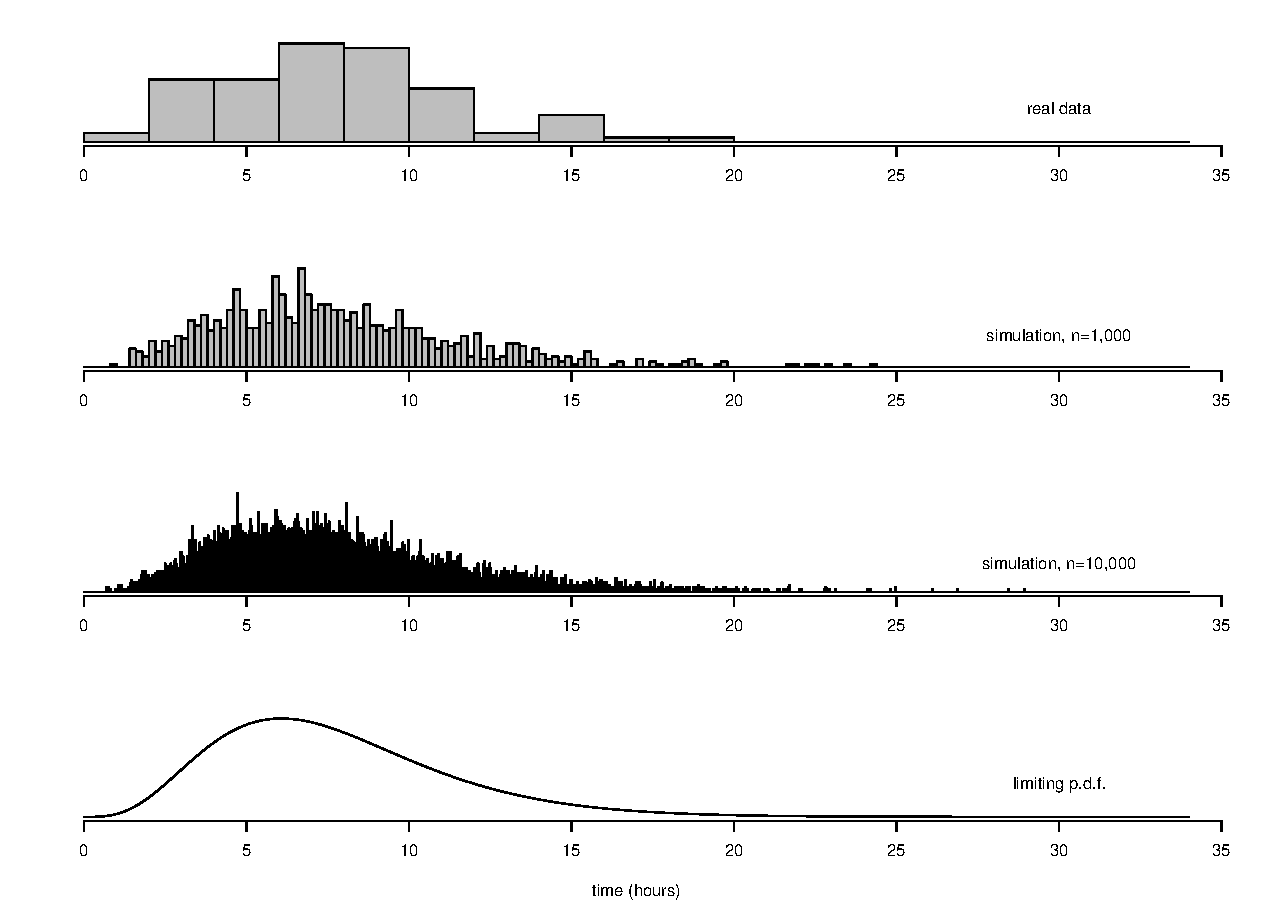
\includegraphics[width=0.75\linewidth]{images/ox_cont_var} 

}

\caption{Top: histogram of the Oxford birth durations. Second from top: histogram of 1,000 values simulated from a distribution fitted to the data. Second from bottom: similarly for 10,000 simulated values. Bottom: p.d.f. of the distribution fitted to the Oxford birth times data.}\label{fig:oxcontvar}
\end{figure}

Suppose that we continue to collect data on birth duration from this hospital, and, as new observations arrive, we add them to the top histogram in Figure \ref{fig:oxcontvar}. We imagine that the times are recorded continuously. As the number of observations \(n\) increases we decrease the bin width of the histogram. As \(n\) increases to infinity the bin width shrinks to zero and the histogram tends to a smooth continuous curve.

This is shown in the bottom 3 plots in Figure \ref{fig:oxcontvar}. The extra data are not real. They are data I have simulated, using a computer, to have a distribution with a similar shape to the histogram of the real data.

Let \(T\) denote the time, in hours, that a woman arriving at the hospital takes to give birth. The smooth continuous curve at the bottom of Figure \ref{fig:oxcontvar} is called the \textbf{probability density function (p.d.f.)} \(f_T(t)\) of the random variable \(T\). Since the total area of the rectangles in a histogram is equal to 1, the area \(\int_{-\infty}^{\infty} f_T(t) \, \mathrm{d}t\) under the p.d.f. \(f_T(t)\) is equal to 1.

\textbf{Definition}. A \textbf{probability density function (p.d.f.)} is a function \(f_{X}(x)\), or simply \(f(x)\), such that

\begin{enumerate}
\def\labelenumi{\arabic{enumi}.}
\tightlist
\item
  \(f_X(x) \geq 0\), for \(-\infty < x < \infty\);
\item
  \(\displaystyle\int_{-\infty}^{\infty} f_X(x) \, \mathrm{d}x = 1\).
\end{enumerate}

Therefore, p.d.f.s are always non-negative and integrate to 1. The support of a continuous random variable is the set of values for which the p.d.f. is positive. Suppose that we wish to find \(P(4 < T \leq 12)\). To find the proportion of times between 4 and 12 using a histogram, we sum the areas of all bins between 4 and 12, that is, we find the area shaded in the histogram in Figure \ref{fig:oxshady}. To do this using the p.d.f. we do effectively the same thing: we find the area under the p.d.f. \(f_T(t)\) between 4 and 12. Since \(f_T(t)\) is a smooth continuous curve, (that is, the bin widths are zero) we integrate \(f_T(t)\) between 4 and 12.

\begin{figure}

{\centering 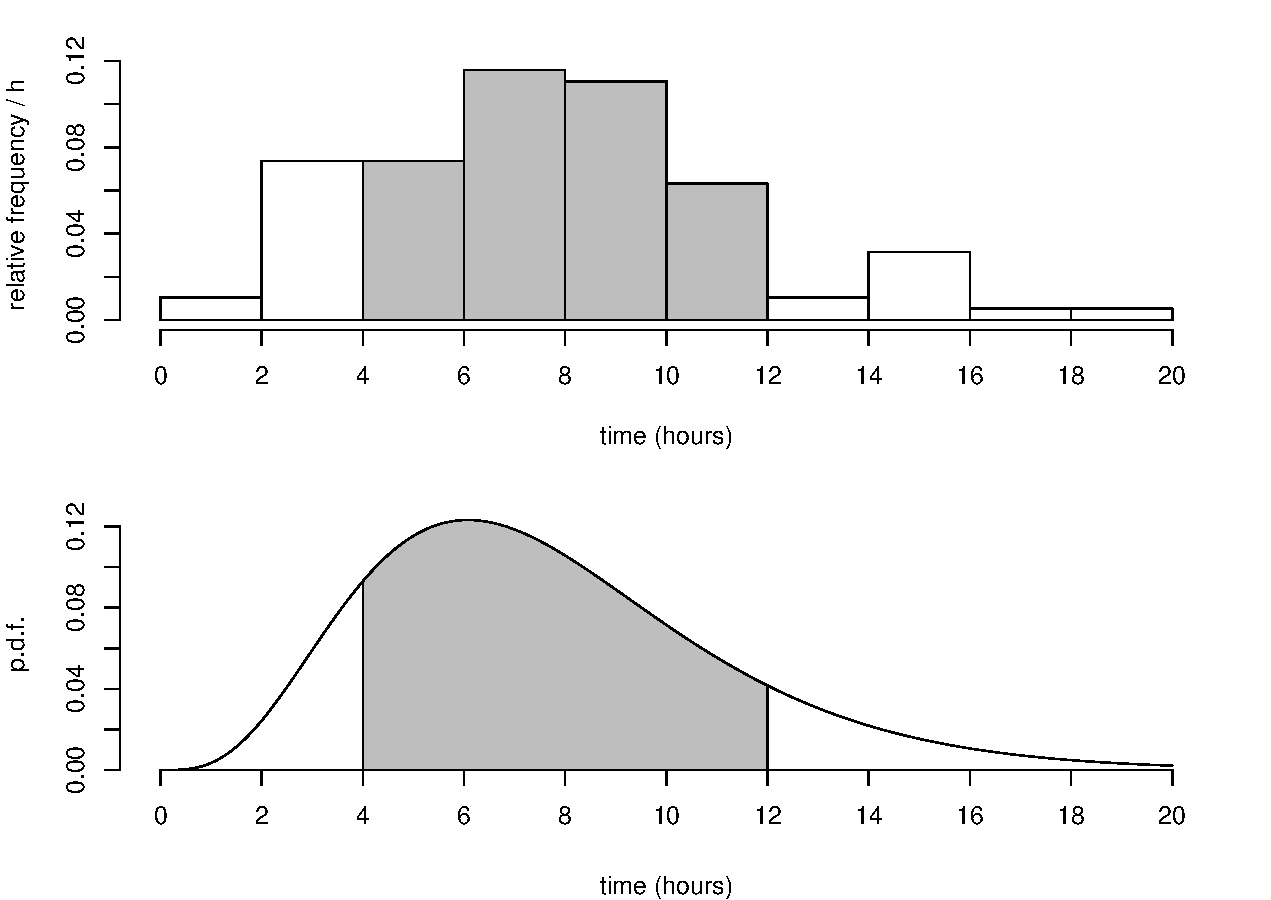
\includegraphics[width=0.75\linewidth]{images/ox_shady} 

}

\caption{Top: histogram of the Oxford birth durations. Bottom: p.d.f. of the distribution fitted to the Oxford birth duration data.}\label{fig:oxshady}
\end{figure}

Therefore
\[ P(4 < T \leq 12) = \displaystyle\int_4^{12} f_T(t) \,\mathrm{d}t = F_T(12)-F_T(4). \]

More generally,
\[ P(a < T \leq b) = \displaystyle\int_a^b f_T(t) \,\mathrm{d}t = F_T(b)-F_T(a). \]

\textbf{Definition}. A random variable \(X\) is a \textbf{continuous random variable} if there exists a p.d.f. \(f_X(x)\) such that
\[
P(a < X \leq b) = \int_{a}^{b} f_X(x) \,\mathrm{d}x,
\]
for all \(a\) and \(b\) such that \(a < b\).

Figure \ref{fig:pdfshady} illustrates the properties of a p.d.f..

\begin{figure}

{\centering 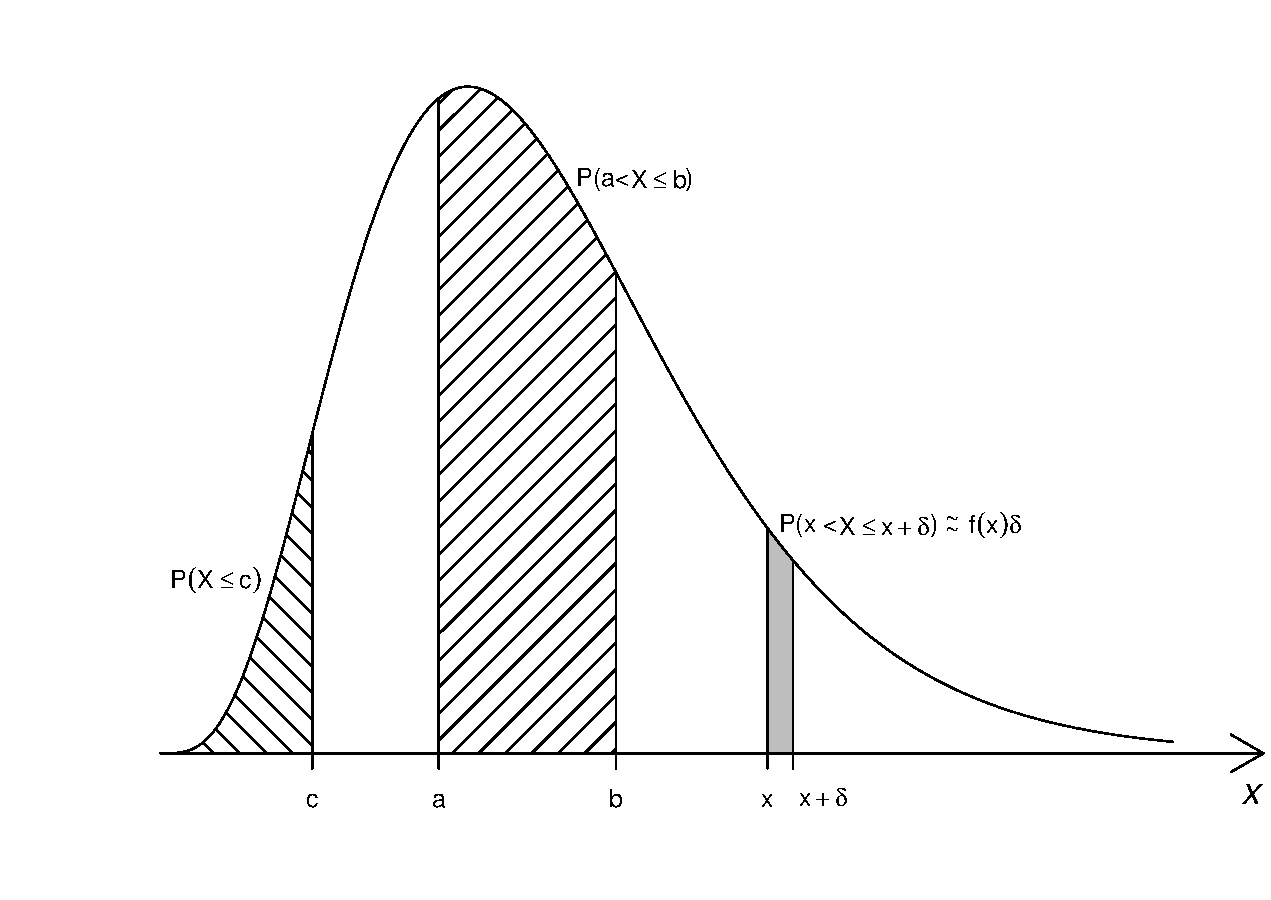
\includegraphics[width=0.75\linewidth]{images/pdf_shady} 

}

\caption{Properties of a p.d.f.. The areas that correspond to the probability that a random variable takes a value in a given interval are shaded.}\label{fig:pdfshady}
\end{figure}

Notes

\begin{itemize}
\tightlist
\item
  It is very important to appreciate that \(f_X(x)\) is \textbf{not} a probability: it does \textbf{not} give \(P(X=x)\). In fact \(P(X=x)=0\): the probability that a continuous random variable \(X\) takes the value \(x\) is zero.
\item
  Indeed, it is possible for a p.d.f. to be greater than 1. Consider a continuous random variable \(X\) with p.d.f.
  \[ f_X(x) = \left\{ \begin{array}{ll} 2\,(1-x) & \,0 \leq x \leq 1, \\ 0 & \,\mbox{otherwise}.\end{array}\right. \]
  For this random variable \(f_X(x)>1\) for any \(x \in [0, 1/2)\) .
\item
  Since \(P(X=x)=0\)
  \[ P(a < X \leq b) = P(a \leq X \leq b) = P(a \leq X < b) = P(a < X < b). \]
\item
  \(f_X(x)\) is a probability \textbf{density}. The probability that \(X\) lies in a very small interval of length \(\delta\) near \(x\) is approximately \(f_X(x) \delta\). For the p.d.f. at the bottom of figure \ref{fig:oxcontvar}, \(f_T(6) > f_T(12)\), indicating that a randomly chosen woman is more likely to spend approximately 6 hours giving birth than approximately
  12 hours.
\end{itemize}

\textbf{Relationship between the c.d.f. and p.d.f. of a continuous random variable}. For a continuous random variable
\[ F_X(x) = P(X \leq x) = \int_{-\infty}^x f_X(u) \,\mathrm{d}u. \]
Therefore,
\[ f_X(x) = \frac{\mathrm{d}}{\mathrm{d}x} F_X(x). \]

\hypertarget{expectation}{%
\section{Expectation}\label{expectation}}

The expectation of a random variable is a measure of the location of its distribution.

\hypertarget{expectation-of-a-discrete-random-variable}{%
\subsection{Expectation of a discrete random variable}\label{expectation-of-a-discrete-random-variable}}

\textbf{Example}. We return to the space shuttle example.

Again we consider test flights conducted at a particular temperature, say 53\(^\circ\)F. Suppose that NASA are able to conduct a very large number \(n\) of test flights at 53\(^\circ\)F, producing a sample \(x_1,\ldots,x_n\) of numbers of damaged O-rings.

Let \(n(x)\) be the number of test flights on which \(x\) of the 6 O-rings were damaged. We can write the sample mean \(\bar{x}\) of \(x_1,\ldots,x_n\) as
\begin{eqnarray*}
\bar{x} &=& \frac{0 \times n(0) + 1 \times n(1) + \cdots + 6 \times n(6)}{n}, \\
&=& \sum_{x=0}^6 x\,\frac{n(x)}{n}.
\end{eqnarray*}
As the sample size \(n\) increases to infinity, the sample proportion \(n(x)/n\) tends to \(P(X=x)\), for \(x=0,1,\ldots,6\). Therefore, in the limit as \(n \rightarrow \infty\), \(\bar{x}\) tends to
\begin{eqnarray}
\sum_{x=0}^6 x\,P(X=x). 
\label{eq:shuttlemean}
\end{eqnarray}
This is known as the mean of the probability distribution of \(X\). It is a measure of the location of the distribution.

The quantity in equation \eqref{eq:shuttlemean} is the value of the sample mean \(\bar{x}\) that we would expect to get from a very large sample. Therefore it is often called the \textbf{expectation} or \textbf{expected value} of the random variable \(X\) and it is denoted \(\mathrm{E}(X)\).

\textbf{Definition}. The \textbf{expectation} (or \textbf{expected value} or \textbf{mean}) \(\mathrm{E}(X)\) of a discrete random variable \(X\) is given by
\begin{eqnarray}
\mathrm{E}(X) &=& \sum_x x\,P(X=x). 
\label{eq:discmean}
\end{eqnarray}
This is a weighted average of the values that \(X\) can take, each value being weighted by \(P(X=x)\).

Note:

\begin{itemize}
\tightlist
\item
  We often write \(\mu\) or \(\mu_X\) for \(\mathrm{E}(X)\).
\item
  Units: the units of \(\mathrm{E}(X)\) are the same as those of \(X\). For example, if \(X\) is measured in hours then \(\mathrm{E}(X)\) is measured in hours.
\item
  \(\mathrm{E}(X)\) exists only if \(\sum_x |x|\,P(X=x) < \infty\). If the number of values \(X\) can take is finite then \(\mathrm{E}(X)\) will always exist.
\end{itemize}

\hypertarget{expectation-of-a-continuous-random-variable}{%
\subsection{Expectation of a continuous random variable}\label{expectation-of-a-continuous-random-variable}}

We can define the expectation of a continuous random variable in a similar way to a discrete random variable, replacing summation with integration.

\textbf{Definition}.
The expectation \(\mathrm{E}(X)\) of a continuous random variable \(X\) is given by
\begin{eqnarray}
\mathrm{E}(X) = \int_{-\infty}^{\infty} x\,f_X(x) \,\mathrm{d}x. 
\label{eq:contmean}
\end{eqnarray}
Note:

\begin{itemize}
\tightlist
\item
  Like the discrete case, this is a weighted average of the values that \(X\) can take, but now each value is weighted by the
  p.d.f. \(f_X(x)\).
\item
  The range of integration in equation \eqref{eq:contmean} is over the whole real line but, in practice, integration will be over the range of possible values of \(X\).
\item
  \(\mathrm{E}(X)\) exists only if \(\int_{-\infty}^{\infty} |x|\,f_X(x) \,\mathrm{d}x < \infty\).
\end{itemize}

\hypertarget{properties-of-mathrmex}{%
\subsection{\texorpdfstring{Properties of \(\mathrm{E}(X)\)}{Properties of \textbackslash mathrm\{E\}(X)}}\label{properties-of-mathrmex}}

If \(a\) and \(b\) are constants then
\[ \mathrm{E}(a\,X+b) = a\,\mathrm{E}(X)+b. \]
This makes sense. If we multiply all observations by \(a\) their mean will also be multiplied by \(a\). If we add \(b\) to all observations their mean will be increased by \(b\), that is, the distribution of \(X\) shifts up by \(b\).

\begin{itemize}
\tightlist
\item
  If \(X \geq 0\) then \(\mathrm{E}(X) \geq 0\).
\item
  If \(X\) is a constant \(c\), that is, \(P(X=c)=1\) then \(\mathrm{E}(X)=c\).
\item
  It can be shown that
  \[ \mathrm{E}(X_1 + X_2 + \cdots + X_n) = \mathrm{E}(X_1) + \mathrm{E}(X_2) + \cdots + \mathrm{E}(X_n). \]
\end{itemize}

\hypertarget{EgX}{%
\subsection{\texorpdfstring{The expectation of \(g(X)\)}{The expectation of g(X)}}\label{EgX}}

Suppose that \(Y=g(X)\) is a function of of \(X\), such as \(aX+b\), \(X^2\) or \(\log X\). Then \(Y\) is also a random variable. If we find the p.m.f (if \(Y\) is discrete) or p.d.f. (if \(Y\) is continuous) of \(Y\) then we can find the expectation of \(Y\) using equation \eqref{eq:discmean} or \eqref{eq:contmean} as appropriate. Alternatively, and often more easily, we can use

\begin{equation}
\mathrm{E}(Y) = \mathrm{E}[g(X)] =
\begin{cases} 
\displaystyle\sum_x g(x)\,P(X=x) & \text{if } X \text{ is discrete}, \\
\int_{-\infty}^{\infty} g(x)\,f_X(x) \,\mathrm{d}x & \text{if } X \text{ is continuous}.
\end{cases}
\label{eq:expfn}
\end{equation}

Note: for a non-linear function \(g(X)\), it is usually the case that
\[ \mathrm{E}[g(X)] \neq g[\mathrm{E}(X)] \]
although there are exceptions.

\hypertarget{variance}{%
\section{Variance}\label{variance}}

The variance of a random variable is a measure of the spread of its distribution.

\hypertarget{variance-of-a-discrete-random-variable}{%
\subsection{Variance of a discrete random variable}\label{variance-of-a-discrete-random-variable}}

\textbf{Example}. We return the space shuttle example.

As before we let \(n(x)\) be the number of test flights on which \(x\) of the 6 O-rings were damaged. We saw in Section \ref{meanstdev} that a measure of the spread of a sample \(x_1,\ldots,x_n\) is the sample variance \(s_X^2\) which, in this example, can be written as

\begin{eqnarray*}
s_X^2 &=& \frac{1}{n-1}\,\left\{
(0-\bar{x})^2\,n(0)+(1-\bar{x})^2\,n(1)+\cdots+(6-\bar{x})^2\,n(6) \right\},
\\
      &=& \sum_{x=0}^6 (x-\bar{x})^2\,\frac{n(x)}{n-1}. 
\end{eqnarray*}
As the sample size \(n\) increases to infinity, \(\frac{n(x)}{n-1}\) tends to \(P(X=x)\), for \(x=0,1,\ldots,6\) and \(\bar{x}\) tends to \(\mu\)=\(\mathrm{E}(X)\).

Therefore, as \(n \rightarrow \infty\), \(s_X^2\) tends to

\begin{equation}
\sum_{x=0}^6 (x-\mu)^2\,P(X=x). 
\label{eq:shuttlevar}
\end{equation}

This is known as the variance of the probability distribution of \(X\). It is a measure of the spread of the distribution. The quantity in equation \eqref{eq:shuttlevar} is the value of the sample variance \(s_X^2\) that we would expect to get from a very large sample.

\textbf{Definition}. The variance \(\mathrm{var}(X)\) of a discrete random variable \(X\) with mean \(\mathrm{E}(X)=\mu\) is given by

\begin{equation}
\mathrm{var}(X) = \sum_x\,(x-\mu)^2\,P(X=x). 
\label{eq:varidisc}
\end{equation}

This is a weighted average of the squared differences between the values that \(X\) can take and its mean \(\mu\), each value being weighted by \(P(X=x)\).

A variance can be infinite. If the number of values that \(X\) can take is finite then \(\mathrm{var}(X)\) will always be finite.

\hypertarget{variance-of-a-continuous-random-variable}{%
\subsection{Variance of a continuous random variable}\label{variance-of-a-continuous-random-variable}}

We can define the variance of a continuous random variable in a similar way to a discrete random variable, replacing summation with integration.

\textbf{Definition}. The variance \(\mathrm{var}(X)\) of a continuous random variable \(X\) with mean \(\mathrm{E}(X)=\mu\) is given by

\begin{equation}
\mathrm{var}(X) = \int_{-\infty}^{\infty} (x-\mu)^2 f_X(x) \,\mathrm{d}x. 
\label{eq:varicont}
\end{equation}

\hypertarget{variance-and-standard-deviation}{%
\subsection{Variance and standard deviation}\label{variance-and-standard-deviation}}

\textbf{Definition}. Let \(X\) be a random variable with \(\mathrm{E}(X)=\mu\). The variance \(\mathrm{var}(X)\) is given by
\[ \mathrm{var}(X) = \mathrm{E}\left[(X-\mu)^2\right]. \]
This follows from equations \eqref{eq:varidisc} and \eqref{eq:varicont} and the expression in equation \eqref{eq:expfn} for the expectation of a function \(g(X)\) of a random variable \(X\).

There is an alternative way to calculate \(\mathrm{var}(X)\):
\[ \mathrm{var}(X) = \mathrm{E}\left(X^2\right) - [\mathrm{E}(X)]^2. \]

\textbf{Exercise}. Prove this.

\textbf{Definition}. The standard deviation sd\((X)\) of \(X\) is given by sd(\(X\))=\(+\sqrt{\mathrm{var}(X)}\).

Notes on \(\mathrm{var}(X)\) and sd(\(X\)):

\begin{itemize}
\tightlist
\item
  \(\mathrm{var}(X) \geq 0\) and \(\mathrm{sd}(X) \geq 0\). Variances and standard deviations cannot be negative.\\
\item
  The units of \(\mathrm{var}(X)\) are the square of those of \(X\). For example, if \(X\) is measured in hours then \(\mathrm{var}(X)\) is measured in hours\(^2\) (and sd(\(X\)) is measured in hours). The units of \(\mathrm{sd}(X)\) are the same as those of \(X\).
\item
  We often write \(\sigma^2\) or \(\sigma_X^2\) for \(\mathrm{var}(X)\) and
  \(\sigma\) or \(\sigma_X\) for \(\mathrm{sd}(X)\).
\item
  \(\mathrm{var}(X)\) exists only if \(\mu\) exists.
\end{itemize}

\hypertarget{properties-of-mathrmvarx}{%
\subsection{\texorpdfstring{Properties of \(\mathrm{var}(X)\)}{Properties of \textbackslash mathrm\{var\}(X)}}\label{properties-of-mathrmvarx}}

\begin{itemize}
\tightlist
\item
  If \(a\) and \(b\) are constants then
  \[ \mathrm{var}(a\,X+b) = a^2\,\mathrm{var}(X). \]
  This makes sense. If we multiply all observations by \(a\) their variance, which is measured square units, will be multiplied by \(a^2\). If we add \(b\) to all observations their variance will be unchanged because the distribution simply shifts up by \(b\) and its spread is unaffected.
\item
  If \(X\) is a constant \(c\), that is, \(P(X=c)=1\) then \(\mathrm{var}(X)=0\): the distribution of \(X\) has zero spread.
\item
  It can also be shown that \textbf{if the random variables \(X_1, X_2, \ldots X_n\) are independent} (see \textbf{An Aside} below) then
\end{itemize}

\begin{equation}
\mathrm{var}(X_1 + X_2 + \cdots + X_n) = \mathrm{var}(X_1) + \mathrm{var}(X_2) + \cdots + \mathrm{var}(X_n). 
\label{eq:varsum}
\end{equation}

\textbf{Note}. Independence is sufficient for this result to hold but it is not necessary. Taking \(n=2\) as an example, in generality we have
\[ \mathrm{var}(X_1 + X_2) = \mathrm{var}(X_1) + \mathrm{var}(X_2) + 2\,\mathrm{cov}(X_1,X_2), \]
where \(\mathrm{cov}(X_1,X_2)\) is the \textbf{covariance} between the random variables \(X_1\) and \(X_2\). Covariance is a measure of the strength of \textbf{linear} association. If \(X_1\) and \(X_2\) are independent (have no association of any kind) then \(\mathrm{cov}(X_1,X_2)=0\), because they have no linear association. However, it is possible for \(X_1\) and \(X_2\) to be dependent but \(\mathrm{cov}(X_1,X_2)=0\), because, although they have some kind of association, they have no \textbf{linear} association. Thus, independence is a stronger requirement than zero covariance.

Returning to general \(n\) we have
\[ \mathrm{var}(X_1 + X_2 + \cdots + X_n) = \mathrm{var}(X_1) + \mathrm{var}(X_2) + \cdots + \mathrm{var}(X_n) + 2 \mathop{\sum\sum}_{i < j} \mathrm{cov}(X_i,X_j). \]
If \(\mathrm{cov}(X_i,X_j)=0\) for all \(i < j\) then equation \eqref{eq:varsum} holds. We will study covariance, and its standardised form \textbf{correlation}, in Chapter \ref{correlationchapter}.

\hypertarget{an-aside}{%
\subsubsection{An aside}\label{an-aside}}

(This is beyond the scope of STAT0002. It is included here for completeness and in case you are interested.) To consider more formally what it means for random variables \(X_1, ..., X_n\) to be independent we define their \textbf{joint c.d.f.} \(F_{X_1, ..., X_n}(x_1, ..., x_n) = P(X_1 \leq x_1, ..., X_n \leq x_n)\). The random variables \(X_1, ..., X_n\) are (mutually) independent if \(F_{X_1, ..., X_n}(x_1, ..., x_n) = F_{X_1}(x_1) \times \cdots \times F_{X_n}(x_n)\), that is, \(P(X_1 \leq x_1, ..., X_n \leq x_n) = P(X_1 \leq x_1) \times \cdots \times P(X_n \leq x_n)\), for any set of values \((x_1, .., x_n)\). The random variables \(X_1, ..., X_n\) are pairwise independent if, \(F_{X_i, X_j}(x_i, x_j) = F_{X_i}(x_i) F_{X_j}(x_j)\), that is, \(P(X_i \leq x_i, X_j \leq x_j) = P(X_i \leq x_i) P(X_j \leq x_j)\), for every pair \((X_i, X_j)\) of variables that we could select from \(X_1, ..., X_n\) and for any pair of values \((x_i, x_j)\).

\hypertarget{locations}{%
\section{Other measures of location}\label{locations}}

\hypertarget{the-median-of-a-random-variable}{%
\subsection{The median of a random variable}\label{the-median-of-a-random-variable}}

Recall that the sample median of a set of observations is the middle observation when the observations are arranged in order of size. We define the median of a random variable \(X\) as a value, median(\(X\)), such that

\[ P(X < \mathrm{median}(X)) \leq \frac12 \leq P(X \leq \mathrm{median}(X)). \]

In other words, \(\mathrm{median}(X)\) is a value where a plot of the c.d.f. \(F_X(x)=P(X \leq x)\) hits \(1/2\).

For a continuous random variable \(X\) we have
\[  F_X(\mathrm{median}(X)) = P(X \leq \mathrm{median}(X)) =\frac12. \]
and a median will divide the distribution into two parts, each with probability 1/2:
\[ P(X < \mathrm{median}(X)) = P(X > \mathrm{median}(X)) = \frac12. \]

This will not necessarily hold for a discrete distribution. For example, suppose that
\[ P(X=0)=\frac16, \qquad  P(X=1)=\frac12, \qquad P(X=2)=\frac13. \]

Then
\begin{eqnarray*}
F_X(x) = P(X \leq x) = \left\{\begin{array}{ll}
0 & \mbox{for } x <0, \\
\frac16 & \mbox{for } 0 \leq x < 1, \\
\frac23 & \mbox{for } 1 \leq x < 2, \\
1 & \mbox{for } x \geq 2, 
\end{array}\right.
\end{eqnarray*}

Figure \ref{fig:discretecdf} is plot of the c.d.f. of this discrete random variable.

\begin{figure}

{\centering \includegraphics[width=0.75\linewidth]{stat0002book_files/figure-latex/discretecdf-1} 

}

\caption{Plot of the c.d.f. of a discrete random variable that takes the values {0, 1, 2} with respective probabilities {1/6, 1/2, 1/3}. The dashed lines indicate the location of the median (1).}\label{fig:discretecdf}
\end{figure}

Therefore, \(\mathrm{median}(X) = 1\). However, \(P(X<1)=\frac16\) and \(P(X>1)=\frac13\).

\hypertarget{the-mode-of-a-random-variable}{%
\subsection{The mode of a random variable}\label{the-mode-of-a-random-variable}}

Recall that the sample mode of categorical or discrete data is the value (or values) which occurs most often. We define the mode, mode(\(X\)), of a random variable as follows.

For a discrete random variable \(X\), the mode is the value which has the highest probability of occurring: \(P(X=\mathrm{mode}(X))\) will be larger than for any other value \(X\) can have. In other words, \(\mathrm{mode}(X)\) is the value at which the p.m.f. is maximised.

For a continuous random variable \(X\), the mode is the value at which the p.d.f. is maximised. \textbf{If the maximum occurs at a turning point of \(f_X(x)\)} then it can be found by solving the equation
\[ \frac{\mathrm{d}}{\mathrm{d}x} f_X(x)  = 0, \]
and checking that you have indeed found a maximum.

\hypertarget{quantiles}{%
\section{Quantiles}\label{quantiles}}

To keep things simple we consider a \textbf{continuous} random variable \(X\). For \(0 < p < 1\), a \(100p\%\) quantile of \(X\) is defined to be a value \(x_p\) such that
\[ F_X(x_p)=P(X \leq x_p) = p. \]
Another way to express this is to say that \(x_p\) is \(F_X^{-1}(p)\), where \(F_X^{-1}\) is the inverse c.d.f. of \(X\). The inverse c.d.f. \(F_X^{-1}\) is also called the quantile function \(Q\) of \(X\), so we could write \(x_p = Q(p)\).

Thus, \(x_{1/4}=F_X^{-1}(1/4)\) is the lower quartile of \(X\), \(x_{1/2}=F_X^{-1}(1/2)\) is the median of \(X\) and \(x_{3/4}=F_X^{-1}(3/4)\) is the upper quartile of \(X\).

The inter-quartile range is \(x_{3/4}-x_{1/4}=F_X^{-1}(3/4)-F_X^{-1}(1/4)\), which is a measure of spread.

\hypertarget{measures-of-shape}{%
\section{Measures of shape}\label{measures-of-shape}}

The \textbf{moment coefficient of skewness} of a random variable \(X\) with mean \(\mu\) and standard deviation \(\sigma\) is given by
\[ \mathrm{E}\left[\left(\frac{X - \mu}{\sigma}\right)^3\right] = \displaystyle\frac{\mathrm{E}\left[\left(X- \mu\right)^3\right]}{\sigma^3}, \]
provided that \(\mathrm{E}[\left(X- \mu\right)^3]\) exists.

The \textbf{quartile skewness} of a random variable \(X\) with c.d.f \(F_X(x)\) is given by
\[ \frac{(x_{3/4}-x_{1/2}) - (x_{1/2}-x_{1/4})}{x_{3/4}-x_{1/4}} = \frac{[F^{-1}_X(3/4) - F^{-1}_X(1/2)] - [F^{-1}_X(1/2) - F^{-1}_X(1/4)]}{F^{-1}_X(3/4) - F^{-1}_X(1/4)}. \]

\hypertarget{simple}{%
\chapter{Simple distributions}\label{simple}}

We use a simple dataset to introduce some commonly-used simple distributions. We will study the \textbf{discrete} distributions: Bernoulli, binomial, geometric and Poisson. We will also study the \textbf{continuous} distributions: uniform, exponential, normal.

\hypertarget{australian-births-data}{%
\section{Australian births data}\label{australian-births-data}}

Steele, S. (December 21, 1997), Babies by the Dozen for Christmas: 24-Hour Baby Boom, The Sunday Mail (Brisbane), page 7

According to this article, a record 44 babies (18 girls and 26 boys) were born in one 24-hour period at the Mater Mothers' Hospital, Brisbane, Australia, on 18th December 1997. The article listed the time of birth, the sex, and the weight in grams for each of the 44 babies. These data are given in Table \ref{tab:abirths}.

 
  \providecommand{\huxb}[2]{\arrayrulecolor[RGB]{#1}\global\arrayrulewidth=#2pt}
  \providecommand{\huxvb}[2]{\color[RGB]{#1}\vrule width #2pt}
  \providecommand{\huxtpad}[1]{\rule{0pt}{#1}}
  \providecommand{\huxbpad}[1]{\rule[-#1]{0pt}{#1}}

\begin{table}[ht]
\begin{centerbox}
\begin{threeparttable}
\captionsetup{justification=centering,singlelinecheck=off}
\caption{\label{tab:abirths} Australian births data.  Times are minutes since midnight.  Weights are in grams.}
 \setlength{\tabcolsep}{0pt}
\begin{tabularx}{0.9\textwidth}{p{0.075\textwidth} p{0.075\textwidth} p{0.075\textwidth} p{0.075\textwidth} p{0.075\textwidth} p{0.075\textwidth} p{0.075\textwidth} p{0.075\textwidth} p{0.075\textwidth} p{0.075\textwidth} p{0.075\textwidth} p{0.075\textwidth}}


\hhline{>{\huxb{0, 0, 0}{3}}=>{\huxb{0, 0, 0}{3}}=>{\huxb{0, 0, 0}{3}}=>{\huxb{0, 0, 0}{3}}=>{\huxb{0, 0, 0}{3}}=>{\huxb{0, 0, 0}{3}}=>{\huxb{0, 0, 0}{3}}=>{\huxb{0, 0, 0}{3}}=>{\huxb{0, 0, 0}{3}}=>{\huxb{0, 0, 0}{3}}=>{\huxb{0, 0, 0}{3}}=>{\huxb{0, 0, 0}{3}}=}
\arrayrulecolor{black}

\multicolumn{1}{!{\huxvb{0, 0, 0}{0}}p{0.075\textwidth}!{\huxvb{0, 0, 0}{0.1}}}{\cellcolor[RGB]{255, 255, 255}\hspace{6pt}\parbox[b]{0.075\textwidth-6pt-6pt}{\huxtpad{0pt + 1em}\centering time\huxbpad{0pt}}} &
\multicolumn{1}{p{0.075\textwidth}!{\huxvb{0, 0, 0}{0.1}}}{\cellcolor[RGB]{255, 255, 255}\hspace{6pt}\parbox[b]{0.075\textwidth-6pt-6pt}{\huxtpad{0pt + 1em}\centering 5\huxbpad{0pt}}} &
\multicolumn{1}{p{0.075\textwidth}!{\huxvb{0, 0, 0}{0.1}}}{\cellcolor[RGB]{255, 255, 255}\hspace{6pt}\parbox[b]{0.075\textwidth-6pt-6pt}{\huxtpad{0pt + 1em}\centering 64\huxbpad{0pt}}} &
\multicolumn{1}{p{0.075\textwidth}!{\huxvb{0, 0, 0}{0.1}}}{\cellcolor[RGB]{255, 255, 255}\hspace{6pt}\parbox[b]{0.075\textwidth-6pt-6pt}{\huxtpad{0pt + 1em}\centering 78\huxbpad{0pt}}} &
\multicolumn{1}{p{0.075\textwidth}!{\huxvb{0, 0, 0}{0.1}}}{\cellcolor[RGB]{255, 255, 255}\hspace{6pt}\parbox[b]{0.075\textwidth-6pt-6pt}{\huxtpad{0pt + 1em}\centering 115\huxbpad{0pt}}} &
\multicolumn{1}{p{0.075\textwidth}!{\huxvb{0, 0, 0}{0.1}}}{\cellcolor[RGB]{255, 255, 255}\hspace{6pt}\parbox[b]{0.075\textwidth-6pt-6pt}{\huxtpad{0pt + 1em}\centering 177\huxbpad{0pt}}} &
\multicolumn{1}{p{0.075\textwidth}!{\huxvb{0, 0, 0}{0.1}}}{\cellcolor[RGB]{255, 255, 255}\hspace{6pt}\parbox[b]{0.075\textwidth-6pt-6pt}{\huxtpad{0pt + 1em}\centering 245\huxbpad{0pt}}} &
\multicolumn{1}{p{0.075\textwidth}!{\huxvb{0, 0, 0}{0.1}}}{\cellcolor[RGB]{255, 255, 255}\hspace{6pt}\parbox[b]{0.075\textwidth-6pt-6pt}{\huxtpad{0pt + 1em}\centering 247\huxbpad{0pt}}} &
\multicolumn{1}{p{0.075\textwidth}!{\huxvb{0, 0, 0}{0.1}}}{\cellcolor[RGB]{255, 255, 255}\hspace{6pt}\parbox[b]{0.075\textwidth-6pt-6pt}{\huxtpad{0pt + 1em}\centering 262\huxbpad{0pt}}} &
\multicolumn{1}{p{0.075\textwidth}!{\huxvb{0, 0, 0}{0.1}}}{\cellcolor[RGB]{255, 255, 255}\hspace{6pt}\parbox[b]{0.075\textwidth-6pt-6pt}{\huxtpad{0pt + 1em}\centering 271\huxbpad{0pt}}} &
\multicolumn{1}{p{0.075\textwidth}!{\huxvb{0, 0, 0}{0.1}}}{\cellcolor[RGB]{255, 255, 255}\hspace{6pt}\parbox[b]{0.075\textwidth-6pt-6pt}{\huxtpad{0pt + 1em}\centering 428\huxbpad{0pt}}} &
\multicolumn{1}{p{0.075\textwidth}!{\huxvb{0, 0, 0}{0}}}{\cellcolor[RGB]{255, 255, 255}\hspace{6pt}\parbox[b]{0.075\textwidth-6pt-6pt}{\huxtpad{0pt + 1em}\centering 455\huxbpad{0pt}}} \tabularnewline[-0.5pt]


\hhline{>{\huxb{0, 0, 0}{0.1}}->{\huxb{0, 0, 0}{0.1}}->{\huxb{0, 0, 0}{0.1}}->{\huxb{0, 0, 0}{0.1}}->{\huxb{0, 0, 0}{0.1}}->{\huxb{0, 0, 0}{0.1}}->{\huxb{0, 0, 0}{0.1}}->{\huxb{0, 0, 0}{0.1}}->{\huxb{0, 0, 0}{0.1}}->{\huxb{0, 0, 0}{0.1}}->{\huxb{0, 0, 0}{0.1}}->{\huxb{0, 0, 0}{0.1}}-}
\arrayrulecolor{black}

\multicolumn{1}{!{\huxvb{0, 0, 0}{0}}p{0.075\textwidth}!{\huxvb{0, 0, 0}{0.1}}}{\cellcolor[RGB]{255, 255, 255}\hspace{6pt}\parbox[b]{0.075\textwidth-6pt-6pt}{\huxtpad{0pt + 1em}\centering sex\huxbpad{0pt}}} &
\multicolumn{1}{p{0.075\textwidth}!{\huxvb{0, 0, 0}{0.1}}}{\cellcolor[RGB]{255, 255, 255}\hspace{6pt}\parbox[b]{0.075\textwidth-6pt-6pt}{\huxtpad{0pt + 1em}\centering girl\huxbpad{0pt}}} &
\multicolumn{1}{p{0.075\textwidth}!{\huxvb{0, 0, 0}{0.1}}}{\cellcolor[RGB]{255, 255, 255}\hspace{6pt}\parbox[b]{0.075\textwidth-6pt-6pt}{\huxtpad{0pt + 1em}\centering girl\huxbpad{0pt}}} &
\multicolumn{1}{p{0.075\textwidth}!{\huxvb{0, 0, 0}{0.1}}}{\cellcolor[RGB]{255, 255, 255}\hspace{6pt}\parbox[b]{0.075\textwidth-6pt-6pt}{\huxtpad{0pt + 1em}\centering boy\huxbpad{0pt}}} &
\multicolumn{1}{p{0.075\textwidth}!{\huxvb{0, 0, 0}{0.1}}}{\cellcolor[RGB]{255, 255, 255}\hspace{6pt}\parbox[b]{0.075\textwidth-6pt-6pt}{\huxtpad{0pt + 1em}\centering boy\huxbpad{0pt}}} &
\multicolumn{1}{p{0.075\textwidth}!{\huxvb{0, 0, 0}{0.1}}}{\cellcolor[RGB]{255, 255, 255}\hspace{6pt}\parbox[b]{0.075\textwidth-6pt-6pt}{\huxtpad{0pt + 1em}\centering boy\huxbpad{0pt}}} &
\multicolumn{1}{p{0.075\textwidth}!{\huxvb{0, 0, 0}{0.1}}}{\cellcolor[RGB]{255, 255, 255}\hspace{6pt}\parbox[b]{0.075\textwidth-6pt-6pt}{\huxtpad{0pt + 1em}\centering girl\huxbpad{0pt}}} &
\multicolumn{1}{p{0.075\textwidth}!{\huxvb{0, 0, 0}{0.1}}}{\cellcolor[RGB]{255, 255, 255}\hspace{6pt}\parbox[b]{0.075\textwidth-6pt-6pt}{\huxtpad{0pt + 1em}\centering girl\huxbpad{0pt}}} &
\multicolumn{1}{p{0.075\textwidth}!{\huxvb{0, 0, 0}{0.1}}}{\cellcolor[RGB]{255, 255, 255}\hspace{6pt}\parbox[b]{0.075\textwidth-6pt-6pt}{\huxtpad{0pt + 1em}\centering boy\huxbpad{0pt}}} &
\multicolumn{1}{p{0.075\textwidth}!{\huxvb{0, 0, 0}{0.1}}}{\cellcolor[RGB]{255, 255, 255}\hspace{6pt}\parbox[b]{0.075\textwidth-6pt-6pt}{\huxtpad{0pt + 1em}\centering boy\huxbpad{0pt}}} &
\multicolumn{1}{p{0.075\textwidth}!{\huxvb{0, 0, 0}{0.1}}}{\cellcolor[RGB]{255, 255, 255}\hspace{6pt}\parbox[b]{0.075\textwidth-6pt-6pt}{\huxtpad{0pt + 1em}\centering boy\huxbpad{0pt}}} &
\multicolumn{1}{p{0.075\textwidth}!{\huxvb{0, 0, 0}{0}}}{\cellcolor[RGB]{255, 255, 255}\hspace{6pt}\parbox[b]{0.075\textwidth-6pt-6pt}{\huxtpad{0pt + 1em}\centering boy\huxbpad{0pt}}} \tabularnewline[-0.5pt]


\hhline{>{\huxb{0, 0, 0}{0.1}}->{\huxb{0, 0, 0}{0.1}}->{\huxb{0, 0, 0}{0.1}}->{\huxb{0, 0, 0}{0.1}}->{\huxb{0, 0, 0}{0.1}}->{\huxb{0, 0, 0}{0.1}}->{\huxb{0, 0, 0}{0.1}}->{\huxb{0, 0, 0}{0.1}}->{\huxb{0, 0, 0}{0.1}}->{\huxb{0, 0, 0}{0.1}}->{\huxb{0, 0, 0}{0.1}}->{\huxb{0, 0, 0}{0.1}}-}
\arrayrulecolor{black}

\multicolumn{1}{!{\huxvb{0, 0, 0}{0}}p{0.075\textwidth}!{\huxvb{0, 0, 0}{0.1}}}{\cellcolor[RGB]{255, 255, 255}\hspace{6pt}\parbox[b]{0.075\textwidth-6pt-6pt}{\huxtpad{0pt + 1em}\centering weight\huxbpad{0pt}}} &
\multicolumn{1}{p{0.075\textwidth}!{\huxvb{0, 0, 0}{0.1}}}{\cellcolor[RGB]{255, 255, 255}\hspace{6pt}\parbox[b]{0.075\textwidth-6pt-6pt}{\huxtpad{0pt + 1em}\centering 3837\huxbpad{0pt}}} &
\multicolumn{1}{p{0.075\textwidth}!{\huxvb{0, 0, 0}{0.1}}}{\cellcolor[RGB]{255, 255, 255}\hspace{6pt}\parbox[b]{0.075\textwidth-6pt-6pt}{\huxtpad{0pt + 1em}\centering 3334\huxbpad{0pt}}} &
\multicolumn{1}{p{0.075\textwidth}!{\huxvb{0, 0, 0}{0.1}}}{\cellcolor[RGB]{255, 255, 255}\hspace{6pt}\parbox[b]{0.075\textwidth-6pt-6pt}{\huxtpad{0pt + 1em}\centering 3554\huxbpad{0pt}}} &
\multicolumn{1}{p{0.075\textwidth}!{\huxvb{0, 0, 0}{0.1}}}{\cellcolor[RGB]{255, 255, 255}\hspace{6pt}\parbox[b]{0.075\textwidth-6pt-6pt}{\huxtpad{0pt + 1em}\centering 3838\huxbpad{0pt}}} &
\multicolumn{1}{p{0.075\textwidth}!{\huxvb{0, 0, 0}{0.1}}}{\cellcolor[RGB]{255, 255, 255}\hspace{6pt}\parbox[b]{0.075\textwidth-6pt-6pt}{\huxtpad{0pt + 1em}\centering 3625\huxbpad{0pt}}} &
\multicolumn{1}{p{0.075\textwidth}!{\huxvb{0, 0, 0}{0.1}}}{\cellcolor[RGB]{255, 255, 255}\hspace{6pt}\parbox[b]{0.075\textwidth-6pt-6pt}{\huxtpad{0pt + 1em}\centering 2208\huxbpad{0pt}}} &
\multicolumn{1}{p{0.075\textwidth}!{\huxvb{0, 0, 0}{0.1}}}{\cellcolor[RGB]{255, 255, 255}\hspace{6pt}\parbox[b]{0.075\textwidth-6pt-6pt}{\huxtpad{0pt + 1em}\centering 1745\huxbpad{0pt}}} &
\multicolumn{1}{p{0.075\textwidth}!{\huxvb{0, 0, 0}{0.1}}}{\cellcolor[RGB]{255, 255, 255}\hspace{6pt}\parbox[b]{0.075\textwidth-6pt-6pt}{\huxtpad{0pt + 1em}\centering 2846\huxbpad{0pt}}} &
\multicolumn{1}{p{0.075\textwidth}!{\huxvb{0, 0, 0}{0.1}}}{\cellcolor[RGB]{255, 255, 255}\hspace{6pt}\parbox[b]{0.075\textwidth-6pt-6pt}{\huxtpad{0pt + 1em}\centering 3166\huxbpad{0pt}}} &
\multicolumn{1}{p{0.075\textwidth}!{\huxvb{0, 0, 0}{0.1}}}{\cellcolor[RGB]{255, 255, 255}\hspace{6pt}\parbox[b]{0.075\textwidth-6pt-6pt}{\huxtpad{0pt + 1em}\centering 3520\huxbpad{0pt}}} &
\multicolumn{1}{p{0.075\textwidth}!{\huxvb{0, 0, 0}{0}}}{\cellcolor[RGB]{255, 255, 255}\hspace{6pt}\parbox[b]{0.075\textwidth-6pt-6pt}{\huxtpad{0pt + 1em}\centering 3380\huxbpad{0pt}}} \tabularnewline[-0.5pt]


\hhline{>{\huxb{0, 0, 0}{3}}=>{\huxb{0, 0, 0}{3}}=>{\huxb{0, 0, 0}{3}}=>{\huxb{0, 0, 0}{3}}=>{\huxb{0, 0, 0}{3}}=>{\huxb{0, 0, 0}{3}}=>{\huxb{0, 0, 0}{3}}=>{\huxb{0, 0, 0}{3}}=>{\huxb{0, 0, 0}{3}}=>{\huxb{0, 0, 0}{3}}=>{\huxb{0, 0, 0}{3}}=>{\huxb{0, 0, 0}{3}}=}
\arrayrulecolor{black}

\multicolumn{1}{!{\huxvb{0, 0, 0}{0}}p{0.075\textwidth}!{\huxvb{0, 0, 0}{0.1}}}{\cellcolor[RGB]{255, 255, 255}\hspace{6pt}\parbox[b]{0.075\textwidth-6pt-6pt}{\huxtpad{0pt + 1em}\centering time\huxbpad{0pt}}} &
\multicolumn{1}{p{0.075\textwidth}!{\huxvb{0, 0, 0}{0.1}}}{\cellcolor[RGB]{255, 255, 255}\hspace{6pt}\parbox[b]{0.075\textwidth-6pt-6pt}{\huxtpad{0pt + 1em}\centering 492\huxbpad{0pt}}} &
\multicolumn{1}{p{0.075\textwidth}!{\huxvb{0, 0, 0}{0.1}}}{\cellcolor[RGB]{255, 255, 255}\hspace{6pt}\parbox[b]{0.075\textwidth-6pt-6pt}{\huxtpad{0pt + 1em}\centering 494\huxbpad{0pt}}} &
\multicolumn{1}{p{0.075\textwidth}!{\huxvb{0, 0, 0}{0.1}}}{\cellcolor[RGB]{255, 255, 255}\hspace{6pt}\parbox[b]{0.075\textwidth-6pt-6pt}{\huxtpad{0pt + 1em}\centering 549\huxbpad{0pt}}} &
\multicolumn{1}{p{0.075\textwidth}!{\huxvb{0, 0, 0}{0.1}}}{\cellcolor[RGB]{255, 255, 255}\hspace{6pt}\parbox[b]{0.075\textwidth-6pt-6pt}{\huxtpad{0pt + 1em}\centering 635\huxbpad{0pt}}} &
\multicolumn{1}{p{0.075\textwidth}!{\huxvb{0, 0, 0}{0.1}}}{\cellcolor[RGB]{255, 255, 255}\hspace{6pt}\parbox[b]{0.075\textwidth-6pt-6pt}{\huxtpad{0pt + 1em}\centering 649\huxbpad{0pt}}} &
\multicolumn{1}{p{0.075\textwidth}!{\huxvb{0, 0, 0}{0.1}}}{\cellcolor[RGB]{255, 255, 255}\hspace{6pt}\parbox[b]{0.075\textwidth-6pt-6pt}{\huxtpad{0pt + 1em}\centering 653\huxbpad{0pt}}} &
\multicolumn{1}{p{0.075\textwidth}!{\huxvb{0, 0, 0}{0.1}}}{\cellcolor[RGB]{255, 255, 255}\hspace{6pt}\parbox[b]{0.075\textwidth-6pt-6pt}{\huxtpad{0pt + 1em}\centering 693\huxbpad{0pt}}} &
\multicolumn{1}{p{0.075\textwidth}!{\huxvb{0, 0, 0}{0.1}}}{\cellcolor[RGB]{255, 255, 255}\hspace{6pt}\parbox[b]{0.075\textwidth-6pt-6pt}{\huxtpad{0pt + 1em}\centering 729\huxbpad{0pt}}} &
\multicolumn{1}{p{0.075\textwidth}!{\huxvb{0, 0, 0}{0.1}}}{\cellcolor[RGB]{255, 255, 255}\hspace{6pt}\parbox[b]{0.075\textwidth-6pt-6pt}{\huxtpad{0pt + 1em}\centering 776\huxbpad{0pt}}} &
\multicolumn{1}{p{0.075\textwidth}!{\huxvb{0, 0, 0}{0.1}}}{\cellcolor[RGB]{255, 255, 255}\hspace{6pt}\parbox[b]{0.075\textwidth-6pt-6pt}{\huxtpad{0pt + 1em}\centering 785\huxbpad{0pt}}} &
\multicolumn{1}{p{0.075\textwidth}!{\huxvb{0, 0, 0}{0}}}{\cellcolor[RGB]{255, 255, 255}\hspace{6pt}\parbox[b]{0.075\textwidth-6pt-6pt}{\huxtpad{0pt + 1em}\centering 846\huxbpad{0pt}}} \tabularnewline[-0.5pt]


\hhline{>{\huxb{0, 0, 0}{0.1}}->{\huxb{0, 0, 0}{0.1}}->{\huxb{0, 0, 0}{0.1}}->{\huxb{0, 0, 0}{0.1}}->{\huxb{0, 0, 0}{0.1}}->{\huxb{0, 0, 0}{0.1}}->{\huxb{0, 0, 0}{0.1}}->{\huxb{0, 0, 0}{0.1}}->{\huxb{0, 0, 0}{0.1}}->{\huxb{0, 0, 0}{0.1}}->{\huxb{0, 0, 0}{0.1}}->{\huxb{0, 0, 0}{0.1}}-}
\arrayrulecolor{black}

\multicolumn{1}{!{\huxvb{0, 0, 0}{0}}p{0.075\textwidth}!{\huxvb{0, 0, 0}{0.1}}}{\cellcolor[RGB]{255, 255, 255}\hspace{6pt}\parbox[b]{0.075\textwidth-6pt-6pt}{\huxtpad{0pt + 1em}\centering sex\huxbpad{0pt}}} &
\multicolumn{1}{p{0.075\textwidth}!{\huxvb{0, 0, 0}{0.1}}}{\cellcolor[RGB]{255, 255, 255}\hspace{6pt}\parbox[b]{0.075\textwidth-6pt-6pt}{\huxtpad{0pt + 1em}\centering boy\huxbpad{0pt}}} &
\multicolumn{1}{p{0.075\textwidth}!{\huxvb{0, 0, 0}{0.1}}}{\cellcolor[RGB]{255, 255, 255}\hspace{6pt}\parbox[b]{0.075\textwidth-6pt-6pt}{\huxtpad{0pt + 1em}\centering girl\huxbpad{0pt}}} &
\multicolumn{1}{p{0.075\textwidth}!{\huxvb{0, 0, 0}{0.1}}}{\cellcolor[RGB]{255, 255, 255}\hspace{6pt}\parbox[b]{0.075\textwidth-6pt-6pt}{\huxtpad{0pt + 1em}\centering girl\huxbpad{0pt}}} &
\multicolumn{1}{p{0.075\textwidth}!{\huxvb{0, 0, 0}{0.1}}}{\cellcolor[RGB]{255, 255, 255}\hspace{6pt}\parbox[b]{0.075\textwidth-6pt-6pt}{\huxtpad{0pt + 1em}\centering boy\huxbpad{0pt}}} &
\multicolumn{1}{p{0.075\textwidth}!{\huxvb{0, 0, 0}{0.1}}}{\cellcolor[RGB]{255, 255, 255}\hspace{6pt}\parbox[b]{0.075\textwidth-6pt-6pt}{\huxtpad{0pt + 1em}\centering girl\huxbpad{0pt}}} &
\multicolumn{1}{p{0.075\textwidth}!{\huxvb{0, 0, 0}{0.1}}}{\cellcolor[RGB]{255, 255, 255}\hspace{6pt}\parbox[b]{0.075\textwidth-6pt-6pt}{\huxtpad{0pt + 1em}\centering girl\huxbpad{0pt}}} &
\multicolumn{1}{p{0.075\textwidth}!{\huxvb{0, 0, 0}{0.1}}}{\cellcolor[RGB]{255, 255, 255}\hspace{6pt}\parbox[b]{0.075\textwidth-6pt-6pt}{\huxtpad{0pt + 1em}\centering boy\huxbpad{0pt}}} &
\multicolumn{1}{p{0.075\textwidth}!{\huxvb{0, 0, 0}{0.1}}}{\cellcolor[RGB]{255, 255, 255}\hspace{6pt}\parbox[b]{0.075\textwidth-6pt-6pt}{\huxtpad{0pt + 1em}\centering boy\huxbpad{0pt}}} &
\multicolumn{1}{p{0.075\textwidth}!{\huxvb{0, 0, 0}{0.1}}}{\cellcolor[RGB]{255, 255, 255}\hspace{6pt}\parbox[b]{0.075\textwidth-6pt-6pt}{\huxtpad{0pt + 1em}\centering boy\huxbpad{0pt}}} &
\multicolumn{1}{p{0.075\textwidth}!{\huxvb{0, 0, 0}{0.1}}}{\cellcolor[RGB]{255, 255, 255}\hspace{6pt}\parbox[b]{0.075\textwidth-6pt-6pt}{\huxtpad{0pt + 1em}\centering boy\huxbpad{0pt}}} &
\multicolumn{1}{p{0.075\textwidth}!{\huxvb{0, 0, 0}{0}}}{\cellcolor[RGB]{255, 255, 255}\hspace{6pt}\parbox[b]{0.075\textwidth-6pt-6pt}{\huxtpad{0pt + 1em}\centering girl\huxbpad{0pt}}} \tabularnewline[-0.5pt]


\hhline{>{\huxb{0, 0, 0}{0.1}}->{\huxb{0, 0, 0}{0.1}}->{\huxb{0, 0, 0}{0.1}}->{\huxb{0, 0, 0}{0.1}}->{\huxb{0, 0, 0}{0.1}}->{\huxb{0, 0, 0}{0.1}}->{\huxb{0, 0, 0}{0.1}}->{\huxb{0, 0, 0}{0.1}}->{\huxb{0, 0, 0}{0.1}}->{\huxb{0, 0, 0}{0.1}}->{\huxb{0, 0, 0}{0.1}}->{\huxb{0, 0, 0}{0.1}}-}
\arrayrulecolor{black}

\multicolumn{1}{!{\huxvb{0, 0, 0}{0}}p{0.075\textwidth}!{\huxvb{0, 0, 0}{0.1}}}{\cellcolor[RGB]{255, 255, 255}\hspace{6pt}\parbox[b]{0.075\textwidth-6pt-6pt}{\huxtpad{0pt + 1em}\centering weight\huxbpad{0pt}}} &
\multicolumn{1}{p{0.075\textwidth}!{\huxvb{0, 0, 0}{0.1}}}{\cellcolor[RGB]{255, 255, 255}\hspace{6pt}\parbox[b]{0.075\textwidth-6pt-6pt}{\huxtpad{0pt + 1em}\centering 3294\huxbpad{0pt}}} &
\multicolumn{1}{p{0.075\textwidth}!{\huxvb{0, 0, 0}{0.1}}}{\cellcolor[RGB]{255, 255, 255}\hspace{6pt}\parbox[b]{0.075\textwidth-6pt-6pt}{\huxtpad{0pt + 1em}\centering 2576\huxbpad{0pt}}} &
\multicolumn{1}{p{0.075\textwidth}!{\huxvb{0, 0, 0}{0.1}}}{\cellcolor[RGB]{255, 255, 255}\hspace{6pt}\parbox[b]{0.075\textwidth-6pt-6pt}{\huxtpad{0pt + 1em}\centering 3208\huxbpad{0pt}}} &
\multicolumn{1}{p{0.075\textwidth}!{\huxvb{0, 0, 0}{0.1}}}{\cellcolor[RGB]{255, 255, 255}\hspace{6pt}\parbox[b]{0.075\textwidth-6pt-6pt}{\huxtpad{0pt + 1em}\centering 3521\huxbpad{0pt}}} &
\multicolumn{1}{p{0.075\textwidth}!{\huxvb{0, 0, 0}{0.1}}}{\cellcolor[RGB]{255, 255, 255}\hspace{6pt}\parbox[b]{0.075\textwidth-6pt-6pt}{\huxtpad{0pt + 1em}\centering 3746\huxbpad{0pt}}} &
\multicolumn{1}{p{0.075\textwidth}!{\huxvb{0, 0, 0}{0.1}}}{\cellcolor[RGB]{255, 255, 255}\hspace{6pt}\parbox[b]{0.075\textwidth-6pt-6pt}{\huxtpad{0pt + 1em}\centering 3523\huxbpad{0pt}}} &
\multicolumn{1}{p{0.075\textwidth}!{\huxvb{0, 0, 0}{0.1}}}{\cellcolor[RGB]{255, 255, 255}\hspace{6pt}\parbox[b]{0.075\textwidth-6pt-6pt}{\huxtpad{0pt + 1em}\centering 2902\huxbpad{0pt}}} &
\multicolumn{1}{p{0.075\textwidth}!{\huxvb{0, 0, 0}{0.1}}}{\cellcolor[RGB]{255, 255, 255}\hspace{6pt}\parbox[b]{0.075\textwidth-6pt-6pt}{\huxtpad{0pt + 1em}\centering 2635\huxbpad{0pt}}} &
\multicolumn{1}{p{0.075\textwidth}!{\huxvb{0, 0, 0}{0.1}}}{\cellcolor[RGB]{255, 255, 255}\hspace{6pt}\parbox[b]{0.075\textwidth-6pt-6pt}{\huxtpad{0pt + 1em}\centering 3920\huxbpad{0pt}}} &
\multicolumn{1}{p{0.075\textwidth}!{\huxvb{0, 0, 0}{0.1}}}{\cellcolor[RGB]{255, 255, 255}\hspace{6pt}\parbox[b]{0.075\textwidth-6pt-6pt}{\huxtpad{0pt + 1em}\centering 3690\huxbpad{0pt}}} &
\multicolumn{1}{p{0.075\textwidth}!{\huxvb{0, 0, 0}{0}}}{\cellcolor[RGB]{255, 255, 255}\hspace{6pt}\parbox[b]{0.075\textwidth-6pt-6pt}{\huxtpad{0pt + 1em}\centering 3430\huxbpad{0pt}}} \tabularnewline[-0.5pt]


\hhline{>{\huxb{0, 0, 0}{3}}=>{\huxb{0, 0, 0}{3}}=>{\huxb{0, 0, 0}{3}}=>{\huxb{0, 0, 0}{3}}=>{\huxb{0, 0, 0}{3}}=>{\huxb{0, 0, 0}{3}}=>{\huxb{0, 0, 0}{3}}=>{\huxb{0, 0, 0}{3}}=>{\huxb{0, 0, 0}{3}}=>{\huxb{0, 0, 0}{3}}=>{\huxb{0, 0, 0}{3}}=>{\huxb{0, 0, 0}{3}}=}
\arrayrulecolor{black}

\multicolumn{1}{!{\huxvb{0, 0, 0}{0}}p{0.075\textwidth}!{\huxvb{0, 0, 0}{0.1}}}{\cellcolor[RGB]{255, 255, 255}\hspace{6pt}\parbox[b]{0.075\textwidth-6pt-6pt}{\huxtpad{0pt + 1em}\centering time\huxbpad{0pt}}} &
\multicolumn{1}{p{0.075\textwidth}!{\huxvb{0, 0, 0}{0.1}}}{\cellcolor[RGB]{255, 255, 255}\hspace{6pt}\parbox[b]{0.075\textwidth-6pt-6pt}{\huxtpad{0pt + 1em}\centering 847\huxbpad{0pt}}} &
\multicolumn{1}{p{0.075\textwidth}!{\huxvb{0, 0, 0}{0.1}}}{\cellcolor[RGB]{255, 255, 255}\hspace{6pt}\parbox[b]{0.075\textwidth-6pt-6pt}{\huxtpad{0pt + 1em}\centering 873\huxbpad{0pt}}} &
\multicolumn{1}{p{0.075\textwidth}!{\huxvb{0, 0, 0}{0.1}}}{\cellcolor[RGB]{255, 255, 255}\hspace{6pt}\parbox[b]{0.075\textwidth-6pt-6pt}{\huxtpad{0pt + 1em}\centering 886\huxbpad{0pt}}} &
\multicolumn{1}{p{0.075\textwidth}!{\huxvb{0, 0, 0}{0.1}}}{\cellcolor[RGB]{255, 255, 255}\hspace{6pt}\parbox[b]{0.075\textwidth-6pt-6pt}{\huxtpad{0pt + 1em}\centering 914\huxbpad{0pt}}} &
\multicolumn{1}{p{0.075\textwidth}!{\huxvb{0, 0, 0}{0.1}}}{\cellcolor[RGB]{255, 255, 255}\hspace{6pt}\parbox[b]{0.075\textwidth-6pt-6pt}{\huxtpad{0pt + 1em}\centering 991\huxbpad{0pt}}} &
\multicolumn{1}{p{0.075\textwidth}!{\huxvb{0, 0, 0}{0.1}}}{\cellcolor[RGB]{255, 255, 255}\hspace{6pt}\parbox[b]{0.075\textwidth-6pt-6pt}{\huxtpad{0pt + 1em}\centering 1017\huxbpad{0pt}}} &
\multicolumn{1}{p{0.075\textwidth}!{\huxvb{0, 0, 0}{0.1}}}{\cellcolor[RGB]{255, 255, 255}\hspace{6pt}\parbox[b]{0.075\textwidth-6pt-6pt}{\huxtpad{0pt + 1em}\centering 1062\huxbpad{0pt}}} &
\multicolumn{1}{p{0.075\textwidth}!{\huxvb{0, 0, 0}{0.1}}}{\cellcolor[RGB]{255, 255, 255}\hspace{6pt}\parbox[b]{0.075\textwidth-6pt-6pt}{\huxtpad{0pt + 1em}\centering 1087\huxbpad{0pt}}} &
\multicolumn{1}{p{0.075\textwidth}!{\huxvb{0, 0, 0}{0.1}}}{\cellcolor[RGB]{255, 255, 255}\hspace{6pt}\parbox[b]{0.075\textwidth-6pt-6pt}{\huxtpad{0pt + 1em}\centering 1105\huxbpad{0pt}}} &
\multicolumn{1}{p{0.075\textwidth}!{\huxvb{0, 0, 0}{0.1}}}{\cellcolor[RGB]{255, 255, 255}\hspace{6pt}\parbox[b]{0.075\textwidth-6pt-6pt}{\huxtpad{0pt + 1em}\centering 1134\huxbpad{0pt}}} &
\multicolumn{1}{p{0.075\textwidth}!{\huxvb{0, 0, 0}{0}}}{\cellcolor[RGB]{255, 255, 255}\hspace{6pt}\parbox[b]{0.075\textwidth-6pt-6pt}{\huxtpad{0pt + 1em}\centering 1149\huxbpad{0pt}}} \tabularnewline[-0.5pt]


\hhline{>{\huxb{0, 0, 0}{0.1}}->{\huxb{0, 0, 0}{0.1}}->{\huxb{0, 0, 0}{0.1}}->{\huxb{0, 0, 0}{0.1}}->{\huxb{0, 0, 0}{0.1}}->{\huxb{0, 0, 0}{0.1}}->{\huxb{0, 0, 0}{0.1}}->{\huxb{0, 0, 0}{0.1}}->{\huxb{0, 0, 0}{0.1}}->{\huxb{0, 0, 0}{0.1}}->{\huxb{0, 0, 0}{0.1}}->{\huxb{0, 0, 0}{0.1}}-}
\arrayrulecolor{black}

\multicolumn{1}{!{\huxvb{0, 0, 0}{0}}p{0.075\textwidth}!{\huxvb{0, 0, 0}{0.1}}}{\cellcolor[RGB]{255, 255, 255}\hspace{6pt}\parbox[b]{0.075\textwidth-6pt-6pt}{\huxtpad{0pt + 1em}\centering sex\huxbpad{0pt}}} &
\multicolumn{1}{p{0.075\textwidth}!{\huxvb{0, 0, 0}{0.1}}}{\cellcolor[RGB]{255, 255, 255}\hspace{6pt}\parbox[b]{0.075\textwidth-6pt-6pt}{\huxtpad{0pt + 1em}\centering girl\huxbpad{0pt}}} &
\multicolumn{1}{p{0.075\textwidth}!{\huxvb{0, 0, 0}{0.1}}}{\cellcolor[RGB]{255, 255, 255}\hspace{6pt}\parbox[b]{0.075\textwidth-6pt-6pt}{\huxtpad{0pt + 1em}\centering girl\huxbpad{0pt}}} &
\multicolumn{1}{p{0.075\textwidth}!{\huxvb{0, 0, 0}{0.1}}}{\cellcolor[RGB]{255, 255, 255}\hspace{6pt}\parbox[b]{0.075\textwidth-6pt-6pt}{\huxtpad{0pt + 1em}\centering girl\huxbpad{0pt}}} &
\multicolumn{1}{p{0.075\textwidth}!{\huxvb{0, 0, 0}{0.1}}}{\cellcolor[RGB]{255, 255, 255}\hspace{6pt}\parbox[b]{0.075\textwidth-6pt-6pt}{\huxtpad{0pt + 1em}\centering boy\huxbpad{0pt}}} &
\multicolumn{1}{p{0.075\textwidth}!{\huxvb{0, 0, 0}{0.1}}}{\cellcolor[RGB]{255, 255, 255}\hspace{6pt}\parbox[b]{0.075\textwidth-6pt-6pt}{\huxtpad{0pt + 1em}\centering boy\huxbpad{0pt}}} &
\multicolumn{1}{p{0.075\textwidth}!{\huxvb{0, 0, 0}{0.1}}}{\cellcolor[RGB]{255, 255, 255}\hspace{6pt}\parbox[b]{0.075\textwidth-6pt-6pt}{\huxtpad{0pt + 1em}\centering boy\huxbpad{0pt}}} &
\multicolumn{1}{p{0.075\textwidth}!{\huxvb{0, 0, 0}{0.1}}}{\cellcolor[RGB]{255, 255, 255}\hspace{6pt}\parbox[b]{0.075\textwidth-6pt-6pt}{\huxtpad{0pt + 1em}\centering girl\huxbpad{0pt}}} &
\multicolumn{1}{p{0.075\textwidth}!{\huxvb{0, 0, 0}{0.1}}}{\cellcolor[RGB]{255, 255, 255}\hspace{6pt}\parbox[b]{0.075\textwidth-6pt-6pt}{\huxtpad{0pt + 1em}\centering boy\huxbpad{0pt}}} &
\multicolumn{1}{p{0.075\textwidth}!{\huxvb{0, 0, 0}{0.1}}}{\cellcolor[RGB]{255, 255, 255}\hspace{6pt}\parbox[b]{0.075\textwidth-6pt-6pt}{\huxtpad{0pt + 1em}\centering girl\huxbpad{0pt}}} &
\multicolumn{1}{p{0.075\textwidth}!{\huxvb{0, 0, 0}{0.1}}}{\cellcolor[RGB]{255, 255, 255}\hspace{6pt}\parbox[b]{0.075\textwidth-6pt-6pt}{\huxtpad{0pt + 1em}\centering boy\huxbpad{0pt}}} &
\multicolumn{1}{p{0.075\textwidth}!{\huxvb{0, 0, 0}{0}}}{\cellcolor[RGB]{255, 255, 255}\hspace{6pt}\parbox[b]{0.075\textwidth-6pt-6pt}{\huxtpad{0pt + 1em}\centering boy\huxbpad{0pt}}} \tabularnewline[-0.5pt]


\hhline{>{\huxb{0, 0, 0}{0.1}}->{\huxb{0, 0, 0}{0.1}}->{\huxb{0, 0, 0}{0.1}}->{\huxb{0, 0, 0}{0.1}}->{\huxb{0, 0, 0}{0.1}}->{\huxb{0, 0, 0}{0.1}}->{\huxb{0, 0, 0}{0.1}}->{\huxb{0, 0, 0}{0.1}}->{\huxb{0, 0, 0}{0.1}}->{\huxb{0, 0, 0}{0.1}}->{\huxb{0, 0, 0}{0.1}}->{\huxb{0, 0, 0}{0.1}}-}
\arrayrulecolor{black}

\multicolumn{1}{!{\huxvb{0, 0, 0}{0}}p{0.075\textwidth}!{\huxvb{0, 0, 0}{0.1}}}{\cellcolor[RGB]{255, 255, 255}\hspace{6pt}\parbox[b]{0.075\textwidth-6pt-6pt}{\huxtpad{0pt + 1em}\centering weight\huxbpad{0pt}}} &
\multicolumn{1}{p{0.075\textwidth}!{\huxvb{0, 0, 0}{0.1}}}{\cellcolor[RGB]{255, 255, 255}\hspace{6pt}\parbox[b]{0.075\textwidth-6pt-6pt}{\huxtpad{0pt + 1em}\centering 3480\huxbpad{0pt}}} &
\multicolumn{1}{p{0.075\textwidth}!{\huxvb{0, 0, 0}{0.1}}}{\cellcolor[RGB]{255, 255, 255}\hspace{6pt}\parbox[b]{0.075\textwidth-6pt-6pt}{\huxtpad{0pt + 1em}\centering 3116\huxbpad{0pt}}} &
\multicolumn{1}{p{0.075\textwidth}!{\huxvb{0, 0, 0}{0.1}}}{\cellcolor[RGB]{255, 255, 255}\hspace{6pt}\parbox[b]{0.075\textwidth-6pt-6pt}{\huxtpad{0pt + 1em}\centering 3428\huxbpad{0pt}}} &
\multicolumn{1}{p{0.075\textwidth}!{\huxvb{0, 0, 0}{0.1}}}{\cellcolor[RGB]{255, 255, 255}\hspace{6pt}\parbox[b]{0.075\textwidth-6pt-6pt}{\huxtpad{0pt + 1em}\centering 3783\huxbpad{0pt}}} &
\multicolumn{1}{p{0.075\textwidth}!{\huxvb{0, 0, 0}{0.1}}}{\cellcolor[RGB]{255, 255, 255}\hspace{6pt}\parbox[b]{0.075\textwidth-6pt-6pt}{\huxtpad{0pt + 1em}\centering 3345\huxbpad{0pt}}} &
\multicolumn{1}{p{0.075\textwidth}!{\huxvb{0, 0, 0}{0.1}}}{\cellcolor[RGB]{255, 255, 255}\hspace{6pt}\parbox[b]{0.075\textwidth-6pt-6pt}{\huxtpad{0pt + 1em}\centering 3034\huxbpad{0pt}}} &
\multicolumn{1}{p{0.075\textwidth}!{\huxvb{0, 0, 0}{0.1}}}{\cellcolor[RGB]{255, 255, 255}\hspace{6pt}\parbox[b]{0.075\textwidth-6pt-6pt}{\huxtpad{0pt + 1em}\centering 2184\huxbpad{0pt}}} &
\multicolumn{1}{p{0.075\textwidth}!{\huxvb{0, 0, 0}{0.1}}}{\cellcolor[RGB]{255, 255, 255}\hspace{6pt}\parbox[b]{0.075\textwidth-6pt-6pt}{\huxtpad{0pt + 1em}\centering 3300\huxbpad{0pt}}} &
\multicolumn{1}{p{0.075\textwidth}!{\huxvb{0, 0, 0}{0.1}}}{\cellcolor[RGB]{255, 255, 255}\hspace{6pt}\parbox[b]{0.075\textwidth-6pt-6pt}{\huxtpad{0pt + 1em}\centering 2383\huxbpad{0pt}}} &
\multicolumn{1}{p{0.075\textwidth}!{\huxvb{0, 0, 0}{0.1}}}{\cellcolor[RGB]{255, 255, 255}\hspace{6pt}\parbox[b]{0.075\textwidth-6pt-6pt}{\huxtpad{0pt + 1em}\centering 3428\huxbpad{0pt}}} &
\multicolumn{1}{p{0.075\textwidth}!{\huxvb{0, 0, 0}{0}}}{\cellcolor[RGB]{255, 255, 255}\hspace{6pt}\parbox[b]{0.075\textwidth-6pt-6pt}{\huxtpad{0pt + 1em}\centering 4162\huxbpad{0pt}}} \tabularnewline[-0.5pt]


\hhline{>{\huxb{0, 0, 0}{3}}=>{\huxb{0, 0, 0}{3}}=>{\huxb{0, 0, 0}{3}}=>{\huxb{0, 0, 0}{3}}=>{\huxb{0, 0, 0}{3}}=>{\huxb{0, 0, 0}{3}}=>{\huxb{0, 0, 0}{3}}=>{\huxb{0, 0, 0}{3}}=>{\huxb{0, 0, 0}{3}}=>{\huxb{0, 0, 0}{3}}=>{\huxb{0, 0, 0}{3}}=>{\huxb{0, 0, 0}{3}}=}
\arrayrulecolor{black}

\multicolumn{1}{!{\huxvb{0, 0, 0}{0}}p{0.075\textwidth}!{\huxvb{0, 0, 0}{0.1}}}{\cellcolor[RGB]{255, 255, 255}\hspace{6pt}\parbox[b]{0.075\textwidth-6pt-6pt}{\huxtpad{0pt + 1em}\centering time\huxbpad{0pt}}} &
\multicolumn{1}{p{0.075\textwidth}!{\huxvb{0, 0, 0}{0.1}}}{\cellcolor[RGB]{255, 255, 255}\hspace{6pt}\parbox[b]{0.075\textwidth-6pt-6pt}{\huxtpad{0pt + 1em}\centering 1187\huxbpad{0pt}}} &
\multicolumn{1}{p{0.075\textwidth}!{\huxvb{0, 0, 0}{0.1}}}{\cellcolor[RGB]{255, 255, 255}\hspace{6pt}\parbox[b]{0.075\textwidth-6pt-6pt}{\huxtpad{0pt + 1em}\centering 1189\huxbpad{0pt}}} &
\multicolumn{1}{p{0.075\textwidth}!{\huxvb{0, 0, 0}{0.1}}}{\cellcolor[RGB]{255, 255, 255}\hspace{6pt}\parbox[b]{0.075\textwidth-6pt-6pt}{\huxtpad{0pt + 1em}\centering 1191\huxbpad{0pt}}} &
\multicolumn{1}{p{0.075\textwidth}!{\huxvb{0, 0, 0}{0.1}}}{\cellcolor[RGB]{255, 255, 255}\hspace{6pt}\parbox[b]{0.075\textwidth-6pt-6pt}{\huxtpad{0pt + 1em}\centering 1210\huxbpad{0pt}}} &
\multicolumn{1}{p{0.075\textwidth}!{\huxvb{0, 0, 0}{0.1}}}{\cellcolor[RGB]{255, 255, 255}\hspace{6pt}\parbox[b]{0.075\textwidth-6pt-6pt}{\huxtpad{0pt + 1em}\centering 1237\huxbpad{0pt}}} &
\multicolumn{1}{p{0.075\textwidth}!{\huxvb{0, 0, 0}{0.1}}}{\cellcolor[RGB]{255, 255, 255}\hspace{6pt}\parbox[b]{0.075\textwidth-6pt-6pt}{\huxtpad{0pt + 1em}\centering 1251\huxbpad{0pt}}} &
\multicolumn{1}{p{0.075\textwidth}!{\huxvb{0, 0, 0}{0.1}}}{\cellcolor[RGB]{255, 255, 255}\hspace{6pt}\parbox[b]{0.075\textwidth-6pt-6pt}{\huxtpad{0pt + 1em}\centering 1264\huxbpad{0pt}}} &
\multicolumn{1}{p{0.075\textwidth}!{\huxvb{0, 0, 0}{0.1}}}{\cellcolor[RGB]{255, 255, 255}\hspace{6pt}\parbox[b]{0.075\textwidth-6pt-6pt}{\huxtpad{0pt + 1em}\centering 1283\huxbpad{0pt}}} &
\multicolumn{1}{p{0.075\textwidth}!{\huxvb{0, 0, 0}{0.1}}}{\cellcolor[RGB]{255, 255, 255}\hspace{6pt}\parbox[b]{0.075\textwidth-6pt-6pt}{\huxtpad{0pt + 1em}\centering 1337\huxbpad{0pt}}} &
\multicolumn{1}{p{0.075\textwidth}!{\huxvb{0, 0, 0}{0.1}}}{\cellcolor[RGB]{255, 255, 255}\hspace{6pt}\parbox[b]{0.075\textwidth-6pt-6pt}{\huxtpad{0pt + 1em}\centering 1407\huxbpad{0pt}}} &
\multicolumn{1}{p{0.075\textwidth}!{\huxvb{0, 0, 0}{0}}}{\cellcolor[RGB]{255, 255, 255}\hspace{6pt}\parbox[b]{0.075\textwidth-6pt-6pt}{\huxtpad{0pt + 1em}\centering 1435\huxbpad{0pt}}} \tabularnewline[-0.5pt]


\hhline{>{\huxb{0, 0, 0}{0.1}}->{\huxb{0, 0, 0}{0.1}}->{\huxb{0, 0, 0}{0.1}}->{\huxb{0, 0, 0}{0.1}}->{\huxb{0, 0, 0}{0.1}}->{\huxb{0, 0, 0}{0.1}}->{\huxb{0, 0, 0}{0.1}}->{\huxb{0, 0, 0}{0.1}}->{\huxb{0, 0, 0}{0.1}}->{\huxb{0, 0, 0}{0.1}}->{\huxb{0, 0, 0}{0.1}}->{\huxb{0, 0, 0}{0.1}}-}
\arrayrulecolor{black}

\multicolumn{1}{!{\huxvb{0, 0, 0}{0}}p{0.075\textwidth}!{\huxvb{0, 0, 0}{0.1}}}{\cellcolor[RGB]{255, 255, 255}\hspace{6pt}\parbox[b]{0.075\textwidth-6pt-6pt}{\huxtpad{0pt + 1em}\centering sex\huxbpad{0pt}}} &
\multicolumn{1}{p{0.075\textwidth}!{\huxvb{0, 0, 0}{0.1}}}{\cellcolor[RGB]{255, 255, 255}\hspace{6pt}\parbox[b]{0.075\textwidth-6pt-6pt}{\huxtpad{0pt + 1em}\centering boy\huxbpad{0pt}}} &
\multicolumn{1}{p{0.075\textwidth}!{\huxvb{0, 0, 0}{0.1}}}{\cellcolor[RGB]{255, 255, 255}\hspace{6pt}\parbox[b]{0.075\textwidth-6pt-6pt}{\huxtpad{0pt + 1em}\centering boy\huxbpad{0pt}}} &
\multicolumn{1}{p{0.075\textwidth}!{\huxvb{0, 0, 0}{0.1}}}{\cellcolor[RGB]{255, 255, 255}\hspace{6pt}\parbox[b]{0.075\textwidth-6pt-6pt}{\huxtpad{0pt + 1em}\centering boy\huxbpad{0pt}}} &
\multicolumn{1}{p{0.075\textwidth}!{\huxvb{0, 0, 0}{0.1}}}{\cellcolor[RGB]{255, 255, 255}\hspace{6pt}\parbox[b]{0.075\textwidth-6pt-6pt}{\huxtpad{0pt + 1em}\centering girl\huxbpad{0pt}}} &
\multicolumn{1}{p{0.075\textwidth}!{\huxvb{0, 0, 0}{0.1}}}{\cellcolor[RGB]{255, 255, 255}\hspace{6pt}\parbox[b]{0.075\textwidth-6pt-6pt}{\huxtpad{0pt + 1em}\centering boy\huxbpad{0pt}}} &
\multicolumn{1}{p{0.075\textwidth}!{\huxvb{0, 0, 0}{0.1}}}{\cellcolor[RGB]{255, 255, 255}\hspace{6pt}\parbox[b]{0.075\textwidth-6pt-6pt}{\huxtpad{0pt + 1em}\centering boy\huxbpad{0pt}}} &
\multicolumn{1}{p{0.075\textwidth}!{\huxvb{0, 0, 0}{0.1}}}{\cellcolor[RGB]{255, 255, 255}\hspace{6pt}\parbox[b]{0.075\textwidth-6pt-6pt}{\huxtpad{0pt + 1em}\centering boy\huxbpad{0pt}}} &
\multicolumn{1}{p{0.075\textwidth}!{\huxvb{0, 0, 0}{0.1}}}{\cellcolor[RGB]{255, 255, 255}\hspace{6pt}\parbox[b]{0.075\textwidth-6pt-6pt}{\huxtpad{0pt + 1em}\centering boy\huxbpad{0pt}}} &
\multicolumn{1}{p{0.075\textwidth}!{\huxvb{0, 0, 0}{0.1}}}{\cellcolor[RGB]{255, 255, 255}\hspace{6pt}\parbox[b]{0.075\textwidth-6pt-6pt}{\huxtpad{0pt + 1em}\centering girl\huxbpad{0pt}}} &
\multicolumn{1}{p{0.075\textwidth}!{\huxvb{0, 0, 0}{0.1}}}{\cellcolor[RGB]{255, 255, 255}\hspace{6pt}\parbox[b]{0.075\textwidth-6pt-6pt}{\huxtpad{0pt + 1em}\centering girl\huxbpad{0pt}}} &
\multicolumn{1}{p{0.075\textwidth}!{\huxvb{0, 0, 0}{0}}}{\cellcolor[RGB]{255, 255, 255}\hspace{6pt}\parbox[b]{0.075\textwidth-6pt-6pt}{\huxtpad{0pt + 1em}\centering girl\huxbpad{0pt}}} \tabularnewline[-0.5pt]


\hhline{>{\huxb{0, 0, 0}{0.1}}->{\huxb{0, 0, 0}{0.1}}->{\huxb{0, 0, 0}{0.1}}->{\huxb{0, 0, 0}{0.1}}->{\huxb{0, 0, 0}{0.1}}->{\huxb{0, 0, 0}{0.1}}->{\huxb{0, 0, 0}{0.1}}->{\huxb{0, 0, 0}{0.1}}->{\huxb{0, 0, 0}{0.1}}->{\huxb{0, 0, 0}{0.1}}->{\huxb{0, 0, 0}{0.1}}->{\huxb{0, 0, 0}{0.1}}-}
\arrayrulecolor{black}

\multicolumn{1}{!{\huxvb{0, 0, 0}{0}}p{0.075\textwidth}!{\huxvb{0, 0, 0}{0.1}}}{\cellcolor[RGB]{255, 255, 255}\hspace{6pt}\parbox[b]{0.075\textwidth-6pt-6pt}{\huxtpad{0pt + 1em}\centering weight\huxbpad{0pt}}} &
\multicolumn{1}{p{0.075\textwidth}!{\huxvb{0, 0, 0}{0.1}}}{\cellcolor[RGB]{255, 255, 255}\hspace{6pt}\parbox[b]{0.075\textwidth-6pt-6pt}{\huxtpad{0pt + 1em}\centering 3630\huxbpad{0pt}}} &
\multicolumn{1}{p{0.075\textwidth}!{\huxvb{0, 0, 0}{0.1}}}{\cellcolor[RGB]{255, 255, 255}\hspace{6pt}\parbox[b]{0.075\textwidth-6pt-6pt}{\huxtpad{0pt + 1em}\centering 3406\huxbpad{0pt}}} &
\multicolumn{1}{p{0.075\textwidth}!{\huxvb{0, 0, 0}{0.1}}}{\cellcolor[RGB]{255, 255, 255}\hspace{6pt}\parbox[b]{0.075\textwidth-6pt-6pt}{\huxtpad{0pt + 1em}\centering 3402\huxbpad{0pt}}} &
\multicolumn{1}{p{0.075\textwidth}!{\huxvb{0, 0, 0}{0.1}}}{\cellcolor[RGB]{255, 255, 255}\hspace{6pt}\parbox[b]{0.075\textwidth-6pt-6pt}{\huxtpad{0pt + 1em}\centering 3500\huxbpad{0pt}}} &
\multicolumn{1}{p{0.075\textwidth}!{\huxvb{0, 0, 0}{0.1}}}{\cellcolor[RGB]{255, 255, 255}\hspace{6pt}\parbox[b]{0.075\textwidth-6pt-6pt}{\huxtpad{0pt + 1em}\centering 3736\huxbpad{0pt}}} &
\multicolumn{1}{p{0.075\textwidth}!{\huxvb{0, 0, 0}{0.1}}}{\cellcolor[RGB]{255, 255, 255}\hspace{6pt}\parbox[b]{0.075\textwidth-6pt-6pt}{\huxtpad{0pt + 1em}\centering 3370\huxbpad{0pt}}} &
\multicolumn{1}{p{0.075\textwidth}!{\huxvb{0, 0, 0}{0.1}}}{\cellcolor[RGB]{255, 255, 255}\hspace{6pt}\parbox[b]{0.075\textwidth-6pt-6pt}{\huxtpad{0pt + 1em}\centering 2121\huxbpad{0pt}}} &
\multicolumn{1}{p{0.075\textwidth}!{\huxvb{0, 0, 0}{0.1}}}{\cellcolor[RGB]{255, 255, 255}\hspace{6pt}\parbox[b]{0.075\textwidth-6pt-6pt}{\huxtpad{0pt + 1em}\centering 3150\huxbpad{0pt}}} &
\multicolumn{1}{p{0.075\textwidth}!{\huxvb{0, 0, 0}{0.1}}}{\cellcolor[RGB]{255, 255, 255}\hspace{6pt}\parbox[b]{0.075\textwidth-6pt-6pt}{\huxtpad{0pt + 1em}\centering 3866\huxbpad{0pt}}} &
\multicolumn{1}{p{0.075\textwidth}!{\huxvb{0, 0, 0}{0.1}}}{\cellcolor[RGB]{255, 255, 255}\hspace{6pt}\parbox[b]{0.075\textwidth-6pt-6pt}{\huxtpad{0pt + 1em}\centering 3542\huxbpad{0pt}}} &
\multicolumn{1}{p{0.075\textwidth}!{\huxvb{0, 0, 0}{0}}}{\cellcolor[RGB]{255, 255, 255}\hspace{6pt}\parbox[b]{0.075\textwidth-6pt-6pt}{\huxtpad{0pt + 1em}\centering 3278\huxbpad{0pt}}} \tabularnewline[-0.5pt]


\hhline{>{\huxb{0, 0, 0}{0.1}}->{\huxb{0, 0, 0}{0.1}}->{\huxb{0, 0, 0}{0.1}}->{\huxb{0, 0, 0}{0.1}}->{\huxb{0, 0, 0}{0.1}}->{\huxb{0, 0, 0}{0.1}}->{\huxb{0, 0, 0}{0.1}}->{\huxb{0, 0, 0}{0.1}}->{\huxb{0, 0, 0}{0.1}}->{\huxb{0, 0, 0}{0.1}}->{\huxb{0, 0, 0}{0.1}}->{\huxb{0, 0, 0}{0.1}}-}
\arrayrulecolor{black}
\end{tabularx}
\end{threeparttable}\par\end{centerbox}

\end{table}
 

Figure \ref{fig:babyintro} summarises the birth times of boy and girl babies.

\begin{figure}

{\centering \includegraphics[width=0.75\linewidth]{images/baby_intro} 

}

\caption{Birth times of babies on 18th December 1997 by sex.}\label{fig:babyintro}
\end{figure}

\hypertarget{the-bernoulli-distribution}{%
\section{The Bernoulli distribution}\label{the-bernoulli-distribution}}

Consider the first birth. The outcome is either a boy \(B\) or a girl \(G\). We define a random variable

\begin{equation}
X_1 =
\begin{cases} 
0 & \text{ if the first baby is a girl} \\
1 & \text{ if the first baby is a boy}.
\end{cases}
\end{equation}

\(X_1\) is the outcome of a \textbf{Bernoulli trial}, that is, an experiment that has two possible outcomes. Here, we have mapped the birth of a girl to the value 0 and the birth of a boy to the value 1. This is arbitrary: we could have done this the other way round.

Let
\begin{eqnarray*}
P(X_1=0)&=&1-p \\
P(X_1=1)&=&p. 
\end{eqnarray*}
Therefore,

\begin{equation}
X_1 =
\begin{cases} 
0 & \text{ with probability (w.p.)} \,\,1-p \\
1 & \text{ with probability (w.p.)} \,\,p.
\end{cases}
\end{equation}

\(X_1\) has a Bernoulli distribution with parameter \(p\), \((0 \leq p \leq 1)\), or, for short,
\[ X_1 \sim
\,\mbox{Bernoulli}(p). 
\]
Here, ``\(\sim\)'' means ``is distributed as''.

Similarly, we define the random variables
\begin{eqnarray*}
X_i &=& \left\{ \begin{array}{ll}0&\mbox{  if the $i$th baby is a girl}; \\
                                 1&\mbox{  if the $i$th baby is a boy,} \quad\mbox{for}\,\,\,i=1,\ldots,44.\end{array}\right.
\end{eqnarray*}
If we assume that the probability of a boy is the same for each birth then
\[ X_i \sim \mbox{Bernoulli}(p), \qquad \mbox{for}\,\,\,i=1,\ldots,44. \]

In this example the sample values \(x_1, \ldots, x_{44}\) of \(X_1,\ldots,X_{44}\) are
\[ x_1=0, \quad x_2=0, \quad x_3=1, \quad \ldots \quad x_{44}=0. \]

\hypertarget{summary-of-the-bernoullip-distribution}{%
\subsection{\texorpdfstring{Summary of the Bernoulli(\(p\)) distribution}{Summary of the Bernoulli(p) distribution}}\label{summary-of-the-bernoullip-distribution}}

\begin{itemize}
\tightlist
\item
  \textbf{Situation}: an experiment with exactly 2 possible outcomes (a Bernoulli trial), mapped to the values 0 and 1.
\item
  If \(X\) is a discrete random variable with p.m.f.
\end{itemize}

\[ P(X=x) \,=\, p^x\,(1-p)^{1-x}, \qquad x=0,1, \]
for some \(p\), \(0 \leq p \leq 1\), then \(X \sim \mbox{Bernoulli}(p)\).

\begin{itemize}
\tightlist
\item
  Parameter: \(p \in [0,1]\).
\item
  \(\mbox{E}(X)=p\), \(\mbox{var}(X)=p\,(1-p)\). (\textbf{Exercise})
\end{itemize}

\hypertarget{binomial}{%
\section{The binomial distribution}\label{binomial}}

We have seen that the 44 births are 44 Bernoulli trials. We define a random variable \(Y\) equal to the total number of boys in the 44 births, that is,
\[ Y = X_1 + X_2 + \cdots + X_{44} = \sum_{i=1}^{44} X_i. \]
We assume that the outcome of each birth is independent of the outcomes of all the other births, that is, the random variables \(X_1, \ldots, X_{44}\) are mutually independent. Therefore, we have assumed that \(X_1, \ldots, X_{44}\) are independent and identically distributed, or i.i.d. for short. `Identically distributed' means that \(X_1, \ldots, X_{44}\) have exactly the same distribution, including the values of any unknown parameters. We may write

\[ X_i \,\stackrel{{\rm i.i.d.}}{\sim}\, \mbox{Bernoulli}(p), \qquad i=1, ... , 44. \]
or
\[ X_i \,\stackrel{{\rm indep}}{\sim}\, \mbox{Bernoulli}(p), \qquad i=1, ... , 44. \]

\(X_1, ... , X_{44}\) are a \textbf{random sample} from a Bernoulli(\(p\)) distribution.

What is \(P(Y=0)\)?

For \(Y=0\) to occur we need all of the 44 births to be girls, that is,
\[ X_1=X_2=\cdots=X_{44}=0.\]

We have assumed that the events \(X_1=0, X_2=0, \ldots, X_{44}=0\) are independent of each other. Using the multiplication rule for independent events gives
\begin{eqnarray*}
P(Y=0)&=&P(X_1=X_2=\cdots=X_{44}=0), \\
      &=&P(X_1=0) \times P(X_2=0) \times \cdots \times P(X_{44}=0), \\
      &=&(1-p) \times (1-p) \times \cdots \times (1-p), \\
      &=&(1-p)^{44}.
\end{eqnarray*}

What is \(P(Y=1)\)?

For \(Y=1\) to occur we need 43 girls and 1 boy to be born. One way for this to happen is
\[ X_1=1, X_2=0, X_3=0, \ldots, X_{44}=0. \]
Under the assumption of independence, this combination of events has probability \(p\,(1-p)^{43}\).
In fact, there are 44 different ways to get \(Y=1\): the 1 boy could be born 1st, 2nd, 3rd, \ldots, 44th.
Therefore,
\[ P(Y=1) = 44\,p\,(1-p)^{43}. \]
We can continue this argument to find that
\[ 
P(Y=y)={44 \choose y} 
p^y\,(1-p)^{44-y}, \qquad y=0,1,\ldots,44. 
\]
The combinatorial term \({44 \choose y}={}^{44}C_y=\frac{44!}{(44-y)!y!}\)
gives the number of ways in which \(y\) boys births can be positioned among the 44 births.

\(Y\) has a binomial distribution with parameters \(44\) and \(p\), \((0 \leq p \leq 1)\), or, for short,
\[ Y \sim \,\mbox{binomial}(44,p). \]
In this example the observed value of \(Y\) is \(y=26\).

As is usually the case, in this example we know the value of the first parameter, the number of trials, but we do not know the value of the second parameter, the probability \(p\) that a trial results in a 1. Suppose that the 44 babies born on 18th December 2007 at this hospital in Brisbane are representative of babies from some wider population, perhaps the population of babies born (or to be born) in a December in Australia in the 21st century. We want to use these data to estimate the probability \(p\) that a baby chosen randomly from this population is a boy, or equivalently, the proportion \(p\) of babies in this population who are boys.

\textbf{Exercise}. We use \(\hat{p} = 26/44\) as an estimate of \(p\). Why is this a sensible estimate?

Putting a ``hat'' \(\hat{}\) on a quantity indicates that the quantity is being estimated using data. Here, \(\hat{p}\) means ``an estimate of \(p\)''.

Figure \ref{fig:babybinompmfs} shows the p.m.f.s of 4 binomial(44,\(p\)) distributions, for different values of \(p\). One way to think about choosing an estimate of \(p\) is to see for which value of \(p\) the observed data are most likely. In this case we have only one sample value, \(y=26\). Looking at Figure \ref{fig:babybinompmfs} we can see that \(y=26\) is very unlikely for \(p=0.1\) and \(p=0.9\), more likely for \(p=0.5\) and even more likely for \(p=\hat{p}\). In addition to making sense because it is the observed proportion of boy babies, \(\hat{p}\) has the property that the observed data are more likely for \(p=\hat{p}\) than for any other value of \(p\).

\begin{figure}

{\centering \includegraphics[width=0.75\linewidth]{images/binom_pmf1} \includegraphics[width=0.75\linewidth]{images/binom_pmf2} \includegraphics[width=0.75\linewidth]{images/binom_pmf3} \includegraphics[width=0.75\linewidth]{images/binom_pmf4} 

}

\caption{Binomial($44,p$) p.m.f.s: $p=0.1$ (top); $p=1/2$ (second from top); $p=0.591$ (second from bottom); $p=0.9$ (bottom).  The sample value $y=26$ has been shaded in black.}\label{fig:babybinompmfs}
\end{figure}

\hypertarget{binominf}{%
\subsection{\texorpdfstring{A brief look at statistical inference about \(p\)}{A brief look at statistical inference about p}}\label{binominf}}

\textbf{This section of the notes is not part of STAT0002. It introduces ideas surrounding hypothesis testing and confidence intervals. If you take STAT0003 then you will cover these ideas in more detail. This section is included because you may find it interesting to think about these ideas now.}

We have observed more boys than girls. If \(p=1/2\) we would expect roughly equal numbers of boys and girls. Even if it is true that \(p=1/2\), we would only occasionally get equal numbers of boys and girls born on each day. We might like to quantify how unlikely is the event of a 26:18 split in 44 independent Bernoulli(1/2) trials. If this is very unlikely we might think that perhaps \(p \neq 1/2\) after all. This is an example of \textbf{statistical inference}, that is, making an inference about the true value of \(p\). We will study statistical inference in Chapter \ref{inference}.

In this example we might want to infer whether or not \(p=0.5\). We wish to judge whether the estimate \(\hat{p}\) is far enough from 0.5 for us to conclude that \(p \neq 0.5\). We need to take into account how reliable (a term that we will use in Chapter \ref{inference} is how \textbf{precise}) the estimation of \(p\) is. For a given true value of \(p\) the larger the sample size \(n\) (here \(n = 44\)) the greater the precision. If you take STAT0003 then you will study this in some detail. Here, we introduce two main approaches to this problem. They will seem rather similar, but there is a subtle difference.

\hypertarget{if-p0.5-then-how-surprising-is-hatp0.591}{%
\subsubsection*{\texorpdfstring{1. If \(p=0.5\) then how surprising is \(\hat{p}=0.591\)?}{1. If p=0.5 then how surprising is \textbackslash hat\{p\}=0.591?}}\label{if-p0.5-then-how-surprising-is-hatp0.591}}
\addcontentsline{toc}{subsubsection}{1. If \(p=0.5\) then how surprising is \(\hat{p}=0.591\)?}

Suppose that the \textbf{null hypothesis} \(H_0: p=0.5\) is true. How unlikely it is that a sample of size \(44\) produces an estimate of \(p\) as far, or further from, 0.5 than \(\hat{p}=0.591\)?

You could think of this as `standing' on the null hypothesis \(H_0\) and looking to see how far away are the data.

If \(p=0.5\), \(P(Y \geq 26\mbox{ or }Y \leq 18) = 0.15+0.15=0.30\). Figure \ref{fig:binominf} illustrates the calculation of this probability. This (the value 0.30 here) is called a \textbf{\(p\)-value}. A \(p\)-value is a measure of our surprise at seeing the data if the null hypothesis is true. The smaller the \(p\)-value the greater our surprise. We could decide to reject the null hypothesis \(H_0\) that \(p=0.5\) if the \(p\)-value is sufficiently small. Otherwise, we do not reject \(H_0\).

\begin{figure}

{\centering \includegraphics[width=0.75\linewidth]{images/binom_inference_1b} 

}

\caption{A binomial($44,1/2$) p.m.f. with the probabilities satisfying $Y$ less than or equal to 18 or greater than or equal to 26 shaded in black.}\label{fig:binominf}
\end{figure}

A traditional cutoff for ``sufficiently small'' is 0.05, but it is not possible to argue that this is generally better than other choices of cutoff. Based on this cutoff we would not reject \(H_0\), because \(0.3 > 0.05\).

\hypertarget{is-p0.5-plausible-based-on-inferences-made-about-p-using-the-data}{%
\subsubsection*{\texorpdfstring{2. Is \(p=0.5\) plausible based on inferences made about \(p\) using the data?}{2. Is p=0.5 plausible based on inferences made about p using the data?}}\label{is-p0.5-plausible-based-on-inferences-made-about-p-using-the-data}}
\addcontentsline{toc}{subsubsection}{2. Is \(p=0.5\) plausible based on inferences made about \(p\) using the data?}

We estimate \(p\) and then see how close the estimate is to 0.5. In this example \(\hat{p}=26/44=0.591\). To quantify whether this is significantly different from 0.5 we can calculate an interval estimate of \(p\), called a \textbf{confidence interval}, and see whether or not this interval contains 0.5. If it does not contain 0.5 then we could decide to reject the null hypothesis \(H_0\) that \(p=0.5\). Otherwise, we do not reject \(H_0\).

You could think of this as `standing' on the data and looking to see how far away is the null hypothesis \(H_0.\)

A confidence interval is a realisation (the observed value) of a random interval that has a certain probability of covering the true value of \(p\). The interval is random because before we collect the data we do not know what the interval will be. For example, A 95\% confidence interval for \(p\) has a probability of 0.95 of covering the true value of \(p\).

An approximate 95\% confidence interval for \(p\) based on these data is \((0.45,0.74)\) which does contain 0.5. Therefore, we do not reject \(H_0\). You can think of a 95\% confidence interval as a range of values of \(p\) that are consistent with the data, in the sense that we would not reject \(H_0: p = p_0\) for any \(p_0\) contained in this interval if we used approach 1. above with a cutoff of 0.05.

In modern Statistics method 2. (\textbf{interval estimation}) is often preferred to 1. (\textbf{hypothesis testing}) because it gives an interval estimate for \(p\) rather than just a decision of whether or not to reject \(H_0: p=0.5\).

\hypertarget{summary-of-the-binomialnp-distribution}{%
\subsection{\texorpdfstring{Summary of the binomial(\(n,p\)) distribution}{Summary of the binomial(n,p) distribution}}\label{summary-of-the-binomialnp-distribution}}

\begin{itemize}
\tightlist
\item
  \textbf{Situation}: the number of 1s in \(n\) independent Bernoulli trials,
  each trial having the same probability \(p\) of obtaining a 1.
\item
  If \(Y\) is a discrete random variable with p.m.f.
  \[ P(Y=y) \,=\, {n \choose y} p^y\,(1-p)^{n-y}, \qquad y=0,1,\ldots,n, \]
  for some \(p\), \(0 \leq p \leq 1\), then \(Y \sim \mbox{binomial}(n,p)\).
\item
  Parameters: \(n\) (usually known) and \(p \in [0,1]\).
\item
  \(\mbox{E}(Y)=n\,p\), \(\mbox{var}(Y)=n\,p\,(1-p)\). (\textbf{Exercise}. Note that \(Y=X_1 + \cdots + X_n\), where \(X_i, i=1, \ldots, n\) are independent Bernoulli(\(p\)) random variables.)
\end{itemize}

A binomial(1,\(p\)) distribution is the same as a Bernoulli(\(p\)) distribution.

\hypertarget{the-geometric-distribution}{%
\section{The geometric distribution}\label{the-geometric-distribution}}

The ordering of the arrivals of the boy and girl babies is
\[ G G B B B G G B B B B B G G B G G B B B B G G G G B B B G B G B B B B B G B B B B G G G \]

Suppose that are interested in the arrival of the 1st baby boy. We define the random variable \(W_1\) to be the number of births up to and including the birth of the 1st boy. In the current example, the 1st boy is born on the 3rd birth, so the sample value of \(W_1\) is \(w_1=3\).

Now we define \(W_2\) to be the number of births, after the birth of the 1st boy, up to and including the birth of the 2nd boy. In this example the sample value of \(W_2\) is \(w_2=1\).

Similarly, we define \(W_i\) to be the number of births, after the birth of the \((i-1)\)th boy, up to and including the birth of the \(i\)th boy.

This leads to values \(w_1, w_2, \ldots, w_{26}\):
\[ 3, 1, 1, 3, 1, 1, 1, 1, 3, 3, 1, 1, 1, 5, 1, 1, 2, 2, 1, 1, 1, 1, 2, 1, 1, 1 \]
The last 3 observations (\(GGG\)) do not contribute here because we do not know when the next boy arrived. The frequencies of these values appear in column 2 of Table \ref{tab:geom}. In column 4 we have divided these \textbf{observed frequencies} by 26 to obtain the \textbf{relative frequencies}. We explain the contents of columns 3 and 5 of this table later.

 
  \providecommand{\huxb}[2]{\arrayrulecolor[RGB]{#1}\global\arrayrulewidth=#2pt}
  \providecommand{\huxvb}[2]{\color[RGB]{#1}\vrule width #2pt}
  \providecommand{\huxtpad}[1]{\rule{0pt}{#1}}
  \providecommand{\huxbpad}[1]{\rule[-#1]{0pt}{#1}}

\begin{table}[ht]
\begin{centerbox}
\begin{threeparttable}
\captionsetup{justification=centering,singlelinecheck=off}
\caption{\label{tab:geom} Observed frequencies and relative frequencies and their fitted values under a geometric(0.591) distribution.}
 \setlength{\tabcolsep}{0pt}
\begin{tabularx}{0.9\textwidth}{p{0.18\textwidth} p{0.18\textwidth} p{0.18\textwidth} p{0.18\textwidth} p{0.18\textwidth}}


\hhline{>{\huxb{255, 255, 255}{0.1}}->{\huxb{255, 255, 255}{0.1}}->{\huxb{255, 255, 255}{0.1}}->{\huxb{255, 255, 255}{0.1}}->{\huxb{255, 255, 255}{0.1}}-}
\arrayrulecolor{black}

\multicolumn{1}{!{\huxvb{0, 0, 0}{0}}p{0.18\textwidth}!{\huxvb{0, 0, 0}{0.1}}}{\cellcolor[RGB]{255, 255, 255}\hspace{6pt}\parbox[b]{0.18\textwidth-6pt-6pt}{\huxtpad{0pt + 1em}\centering number of births\huxbpad{0pt}}} &
\multicolumn{1}{p{0.18\textwidth}!{\huxvb{0, 0, 0}{0.1}}}{\cellcolor[RGB]{255, 255, 255}\hspace{6pt}\parbox[b]{0.18\textwidth-6pt-6pt}{\huxtpad{0pt + 1em}\centering observed\huxbpad{0pt}}} &
\multicolumn{1}{p{0.18\textwidth}!{\huxvb{0, 0, 0}{0.1}}}{\cellcolor[RGB]{255, 255, 255}\hspace{6pt}\parbox[b]{0.18\textwidth-6pt-6pt}{\huxtpad{0pt + 1em}\centering estimated expected\huxbpad{0pt}}} &
\multicolumn{1}{p{0.18\textwidth}!{\huxvb{0, 0, 0}{0.1}}}{\cellcolor[RGB]{255, 255, 255}\hspace{6pt}\parbox[b]{0.18\textwidth-6pt-6pt}{\huxtpad{0pt + 1em}\centering relative\huxbpad{0pt}}} &
\multicolumn{1}{p{0.18\textwidth}!{\huxvb{0, 0, 0}{0}}}{\cellcolor[RGB]{255, 255, 255}\hspace{6pt}\parbox[b]{0.18\textwidth-6pt-6pt}{\huxtpad{0pt + 1em}\centering estimated\huxbpad{0pt}}} \tabularnewline[-0.5pt]


\hhline{>{\huxb{255, 255, 255}{0.1}}->{\huxb{255, 255, 255}{0.1}}->{\huxb{255, 255, 255}{0.1}}->{\huxb{255, 255, 255}{0.1}}->{\huxb{255, 255, 255}{0.1}}-}
\arrayrulecolor{black}

\multicolumn{1}{!{\huxvb{0, 0, 0}{0}}p{0.18\textwidth}!{\huxvb{0, 0, 0}{0.1}}}{\cellcolor[RGB]{255, 255, 255}\hspace{6pt}\parbox[b]{0.18\textwidth-6pt-6pt}{\huxtpad{0pt + 1em}\centering until boy born\huxbpad{0pt}}} &
\multicolumn{1}{p{0.18\textwidth}!{\huxvb{0, 0, 0}{0.1}}}{\cellcolor[RGB]{255, 255, 255}\hspace{6pt}\parbox[b]{0.18\textwidth-6pt-6pt}{\huxtpad{0pt + 1em}\centering frequency\huxbpad{0pt}}} &
\multicolumn{1}{p{0.18\textwidth}!{\huxvb{0, 0, 0}{0.1}}}{\cellcolor[RGB]{255, 255, 255}\hspace{6pt}\parbox[b]{0.18\textwidth-6pt-6pt}{\huxtpad{0pt + 1em}\centering frequency\huxbpad{0pt}}} &
\multicolumn{1}{p{0.18\textwidth}!{\huxvb{0, 0, 0}{0.1}}}{\cellcolor[RGB]{255, 255, 255}\hspace{6pt}\parbox[b]{0.18\textwidth-6pt-6pt}{\huxtpad{0pt + 1em}\centering frequency\huxbpad{0pt}}} &
\multicolumn{1}{p{0.18\textwidth}!{\huxvb{0, 0, 0}{0}}}{\cellcolor[RGB]{255, 255, 255}\hspace{6pt}\parbox[b]{0.18\textwidth-6pt-6pt}{\huxtpad{0pt + 1em}\centering probability\huxbpad{0pt}}} \tabularnewline[-0.5pt]


\hhline{>{\huxb{0, 0, 0}{0.1}}->{\huxb{0, 0, 0}{0.1}}->{\huxb{0, 0, 0}{0.1}}->{\huxb{0, 0, 0}{0.1}}->{\huxb{0, 0, 0}{0.1}}-}
\arrayrulecolor{black}

\multicolumn{1}{!{\huxvb{0, 0, 0}{0}}p{0.18\textwidth}!{\huxvb{0, 0, 0}{0.1}}}{\cellcolor[RGB]{255, 255, 255}\hspace{6pt}\parbox[b]{0.18\textwidth-6pt-6pt}{\huxtpad{0pt + 1em}\centering 1\huxbpad{0pt}}} &
\multicolumn{1}{p{0.18\textwidth}!{\huxvb{0, 0, 0}{0.1}}}{\cellcolor[RGB]{255, 255, 255}\hspace{6pt}\parbox[b]{0.18\textwidth-6pt-6pt}{\huxtpad{0pt + 1em}\centering 18\huxbpad{0pt}}} &
\multicolumn{1}{p{0.18\textwidth}!{\huxvb{0, 0, 0}{0.1}}}{\cellcolor[RGB]{255, 255, 255}\hspace{6pt}\parbox[b]{0.18\textwidth-6pt-60pt}{\huxtpad{0pt + 1em}\raggedleft 15.36\huxbpad{0pt}}} &
\multicolumn{1}{p{0.18\textwidth}!{\huxvb{0, 0, 0}{0.1}}}{\cellcolor[RGB]{255, 255, 255}\hspace{6pt}\parbox[b]{0.18\textwidth-6pt-6pt}{\huxtpad{0pt + 1em}\centering 0.69\huxbpad{0pt}}} &
\multicolumn{1}{p{0.18\textwidth}!{\huxvb{0, 0, 0}{0}}}{\cellcolor[RGB]{255, 255, 255}\hspace{6pt}\parbox[b]{0.18\textwidth-6pt-6pt}{\huxtpad{0pt + 1em}\centering 0.59\huxbpad{0pt}}} \tabularnewline[-0.5pt]


\hhline{>{\huxb{255, 255, 255}{0.1}}->{\huxb{255, 255, 255}{0.1}}->{\huxb{255, 255, 255}{0.1}}->{\huxb{255, 255, 255}{0.1}}->{\huxb{255, 255, 255}{0.1}}-}
\arrayrulecolor{black}

\multicolumn{1}{!{\huxvb{0, 0, 0}{0}}p{0.18\textwidth}!{\huxvb{0, 0, 0}{0.1}}}{\cellcolor[RGB]{255, 255, 255}\hspace{6pt}\parbox[b]{0.18\textwidth-6pt-6pt}{\huxtpad{0pt + 1em}\centering 2\huxbpad{0pt}}} &
\multicolumn{1}{p{0.18\textwidth}!{\huxvb{0, 0, 0}{0.1}}}{\cellcolor[RGB]{255, 255, 255}\hspace{6pt}\parbox[b]{0.18\textwidth-6pt-6pt}{\huxtpad{0pt + 1em}\centering 3\huxbpad{0pt}}} &
\multicolumn{1}{p{0.18\textwidth}!{\huxvb{0, 0, 0}{0.1}}}{\cellcolor[RGB]{255, 255, 255}\hspace{6pt}\parbox[b]{0.18\textwidth-6pt-60pt}{\huxtpad{0pt + 1em}\raggedleft 6.28\huxbpad{0pt}}} &
\multicolumn{1}{p{0.18\textwidth}!{\huxvb{0, 0, 0}{0.1}}}{\cellcolor[RGB]{255, 255, 255}\hspace{6pt}\parbox[b]{0.18\textwidth-6pt-6pt}{\huxtpad{0pt + 1em}\centering 0.12\huxbpad{0pt}}} &
\multicolumn{1}{p{0.18\textwidth}!{\huxvb{0, 0, 0}{0}}}{\cellcolor[RGB]{255, 255, 255}\hspace{6pt}\parbox[b]{0.18\textwidth-6pt-6pt}{\huxtpad{0pt + 1em}\centering 0.24\huxbpad{0pt}}} \tabularnewline[-0.5pt]


\hhline{>{\huxb{255, 255, 255}{0.1}}->{\huxb{255, 255, 255}{0.1}}->{\huxb{255, 255, 255}{0.1}}->{\huxb{255, 255, 255}{0.1}}->{\huxb{255, 255, 255}{0.1}}-}
\arrayrulecolor{black}

\multicolumn{1}{!{\huxvb{0, 0, 0}{0}}p{0.18\textwidth}!{\huxvb{0, 0, 0}{0.1}}}{\cellcolor[RGB]{255, 255, 255}\hspace{6pt}\parbox[b]{0.18\textwidth-6pt-6pt}{\huxtpad{0pt + 1em}\centering 3\huxbpad{0pt}}} &
\multicolumn{1}{p{0.18\textwidth}!{\huxvb{0, 0, 0}{0.1}}}{\cellcolor[RGB]{255, 255, 255}\hspace{6pt}\parbox[b]{0.18\textwidth-6pt-6pt}{\huxtpad{0pt + 1em}\centering 4\huxbpad{0pt}}} &
\multicolumn{1}{p{0.18\textwidth}!{\huxvb{0, 0, 0}{0.1}}}{\cellcolor[RGB]{255, 255, 255}\hspace{6pt}\parbox[b]{0.18\textwidth-6pt-60pt}{\huxtpad{0pt + 1em}\raggedleft 2.57\huxbpad{0pt}}} &
\multicolumn{1}{p{0.18\textwidth}!{\huxvb{0, 0, 0}{0.1}}}{\cellcolor[RGB]{255, 255, 255}\hspace{6pt}\parbox[b]{0.18\textwidth-6pt-6pt}{\huxtpad{0pt + 1em}\centering 0.15\huxbpad{0pt}}} &
\multicolumn{1}{p{0.18\textwidth}!{\huxvb{0, 0, 0}{0}}}{\cellcolor[RGB]{255, 255, 255}\hspace{6pt}\parbox[b]{0.18\textwidth-6pt-6pt}{\huxtpad{0pt + 1em}\centering 0.10\huxbpad{0pt}}} \tabularnewline[-0.5pt]


\hhline{>{\huxb{255, 255, 255}{0.1}}->{\huxb{255, 255, 255}{0.1}}->{\huxb{255, 255, 255}{0.1}}->{\huxb{255, 255, 255}{0.1}}->{\huxb{255, 255, 255}{0.1}}-}
\arrayrulecolor{black}

\multicolumn{1}{!{\huxvb{0, 0, 0}{0}}p{0.18\textwidth}!{\huxvb{0, 0, 0}{0.1}}}{\cellcolor[RGB]{255, 255, 255}\hspace{6pt}\parbox[b]{0.18\textwidth-6pt-6pt}{\huxtpad{0pt + 1em}\centering 4\huxbpad{0pt}}} &
\multicolumn{1}{p{0.18\textwidth}!{\huxvb{0, 0, 0}{0.1}}}{\cellcolor[RGB]{255, 255, 255}\hspace{6pt}\parbox[b]{0.18\textwidth-6pt-6pt}{\huxtpad{0pt + 1em}\centering 0\huxbpad{0pt}}} &
\multicolumn{1}{p{0.18\textwidth}!{\huxvb{0, 0, 0}{0.1}}}{\cellcolor[RGB]{255, 255, 255}\hspace{6pt}\parbox[b]{0.18\textwidth-6pt-60pt}{\huxtpad{0pt + 1em}\raggedleft 1.05\huxbpad{0pt}}} &
\multicolumn{1}{p{0.18\textwidth}!{\huxvb{0, 0, 0}{0.1}}}{\cellcolor[RGB]{255, 255, 255}\hspace{6pt}\parbox[b]{0.18\textwidth-6pt-6pt}{\huxtpad{0pt + 1em}\centering 0.00\huxbpad{0pt}}} &
\multicolumn{1}{p{0.18\textwidth}!{\huxvb{0, 0, 0}{0}}}{\cellcolor[RGB]{255, 255, 255}\hspace{6pt}\parbox[b]{0.18\textwidth-6pt-6pt}{\huxtpad{0pt + 1em}\centering 0.04\huxbpad{0pt}}} \tabularnewline[-0.5pt]


\hhline{>{\huxb{255, 255, 255}{0.1}}->{\huxb{255, 255, 255}{0.1}}->{\huxb{255, 255, 255}{0.1}}->{\huxb{255, 255, 255}{0.1}}->{\huxb{255, 255, 255}{0.1}}-}
\arrayrulecolor{black}

\multicolumn{1}{!{\huxvb{0, 0, 0}{0}}p{0.18\textwidth}!{\huxvb{0, 0, 0}{0.1}}}{\cellcolor[RGB]{255, 255, 255}\hspace{6pt}\parbox[b]{0.18\textwidth-6pt-6pt}{\huxtpad{0pt + 1em}\centering 5\huxbpad{0pt}}} &
\multicolumn{1}{p{0.18\textwidth}!{\huxvb{0, 0, 0}{0.1}}}{\cellcolor[RGB]{255, 255, 255}\hspace{6pt}\parbox[b]{0.18\textwidth-6pt-6pt}{\huxtpad{0pt + 1em}\centering 1\huxbpad{0pt}}} &
\multicolumn{1}{p{0.18\textwidth}!{\huxvb{0, 0, 0}{0.1}}}{\cellcolor[RGB]{255, 255, 255}\hspace{6pt}\parbox[b]{0.18\textwidth-6pt-60pt}{\huxtpad{0pt + 1em}\raggedleft 0.43\huxbpad{0pt}}} &
\multicolumn{1}{p{0.18\textwidth}!{\huxvb{0, 0, 0}{0.1}}}{\cellcolor[RGB]{255, 255, 255}\hspace{6pt}\parbox[b]{0.18\textwidth-6pt-6pt}{\huxtpad{0pt + 1em}\centering 0.04\huxbpad{0pt}}} &
\multicolumn{1}{p{0.18\textwidth}!{\huxvb{0, 0, 0}{0}}}{\cellcolor[RGB]{255, 255, 255}\hspace{6pt}\parbox[b]{0.18\textwidth-6pt-6pt}{\huxtpad{0pt + 1em}\centering 0.02\huxbpad{0pt}}} \tabularnewline[-0.5pt]


\hhline{>{\huxb{255, 255, 255}{0.1}}->{\huxb{255, 255, 255}{0.1}}->{\huxb{255, 255, 255}{0.1}}->{\huxb{255, 255, 255}{0.1}}->{\huxb{255, 255, 255}{0.1}}-}
\arrayrulecolor{black}

\multicolumn{1}{!{\huxvb{0, 0, 0}{0}}p{0.18\textwidth}!{\huxvb{0, 0, 0}{0.1}}}{\cellcolor[RGB]{255, 255, 255}\hspace{6pt}\parbox[b]{0.18\textwidth-6pt-6pt}{\huxtpad{0pt + 1em}\centering 6+\huxbpad{0pt}}} &
\multicolumn{1}{p{0.18\textwidth}!{\huxvb{0, 0, 0}{0.1}}}{\cellcolor[RGB]{255, 255, 255}\hspace{6pt}\parbox[b]{0.18\textwidth-6pt-6pt}{\huxtpad{0pt + 1em}\centering 0\huxbpad{0pt}}} &
\multicolumn{1}{p{0.18\textwidth}!{\huxvb{0, 0, 0}{0.1}}}{\cellcolor[RGB]{255, 255, 255}\hspace{6pt}\parbox[b]{0.18\textwidth-6pt-60pt}{\huxtpad{0pt + 1em}\raggedleft 0.30\huxbpad{0pt}}} &
\multicolumn{1}{p{0.18\textwidth}!{\huxvb{0, 0, 0}{0.1}}}{\cellcolor[RGB]{255, 255, 255}\hspace{6pt}\parbox[b]{0.18\textwidth-6pt-6pt}{\huxtpad{0pt + 1em}\centering 0.00\huxbpad{0pt}}} &
\multicolumn{1}{p{0.18\textwidth}!{\huxvb{0, 0, 0}{0}}}{\cellcolor[RGB]{255, 255, 255}\hspace{6pt}\parbox[b]{0.18\textwidth-6pt-6pt}{\huxtpad{0pt + 1em}\centering 0.01\huxbpad{0pt}}} \tabularnewline[-0.5pt]


\hhline{>{\huxb{0, 0, 0}{0.1}}->{\huxb{0, 0, 0}{0.1}}->{\huxb{0, 0, 0}{0.1}}->{\huxb{0, 0, 0}{0.1}}->{\huxb{0, 0, 0}{0.1}}-}
\arrayrulecolor{black}

\multicolumn{1}{!{\huxvb{0, 0, 0}{0}}p{0.18\textwidth}!{\huxvb{0, 0, 0}{0.1}}}{\cellcolor[RGB]{255, 255, 255}\hspace{6pt}\parbox[b]{0.18\textwidth-6pt-6pt}{\huxtpad{0pt + 1em}\centering total\huxbpad{0pt}}} &
\multicolumn{1}{p{0.18\textwidth}!{\huxvb{0, 0, 0}{0.1}}}{\cellcolor[RGB]{255, 255, 255}\hspace{6pt}\parbox[b]{0.18\textwidth-6pt-6pt}{\huxtpad{0pt + 1em}\centering 26\huxbpad{0pt}}} &
\multicolumn{1}{p{0.18\textwidth}!{\huxvb{0, 0, 0}{0.1}}}{\cellcolor[RGB]{255, 255, 255}\hspace{6pt}\parbox[b]{0.18\textwidth-6pt-60pt}{\huxtpad{0pt + 1em}\raggedleft 26\hphantom{0}\hphantom{0}\hphantom{0}\huxbpad{0pt}}} &
\multicolumn{1}{p{0.18\textwidth}!{\huxvb{0, 0, 0}{0.1}}}{\cellcolor[RGB]{255, 255, 255}\hspace{6pt}\parbox[b]{0.18\textwidth-6pt-6pt}{\huxtpad{0pt + 1em}\centering 1\huxbpad{0pt}}} &
\multicolumn{1}{p{0.18\textwidth}!{\huxvb{0, 0, 0}{0}}}{\cellcolor[RGB]{255, 255, 255}\hspace{6pt}\parbox[b]{0.18\textwidth-6pt-6pt}{\huxtpad{0pt + 1em}\centering 1\huxbpad{0pt}}} \tabularnewline[-0.5pt]


\hhline{>{\huxb{0, 0, 0}{0.1}}|>{\huxb{0, 0, 0}{0.1}}|>{\huxb{0, 0, 0}{0.1}}|>{\huxb{0, 0, 0}{0.1}}|}
\arrayrulecolor{black}
\end{tabularx}
\end{threeparttable}\par\end{centerbox}

\end{table}
 

\textbf{Question}: Why have I written `\(\geq\) 6' in the first column of Table \ref{tab:geom} rather than `6'?

The observed frequencies are plotted in Figure \ref{fig:geombar}.

\begin{figure}

{\centering \includegraphics[width=0.75\linewidth]{images/baby_geom_bar} 

}

\caption{Bar plot of numbers of births between successive baby boys (including the next baby boy).}\label{fig:geombar}
\end{figure}

Now we find the probability distribution of \(W_1, W_2, \ldots\). First we consider \(W_1\). Recall that the outcomes \(X_1,\ldots,X_{44}\) of the 44 births are assumed to be independent Bernoulli trials.

What is \(P(W_1=1)\)?.

For \(W_1=1\) to occur we need the next birth to be a boy. Therefore, \(P(W_1=1)=p\).

What is \(P(W_1=2)\)?.

For \(W_1=2\) to occur we need a girl followed by a boy. Therefore, \(P(W_1=2)=(1-p)\,p\).

We can continue this argument to find

\begin{equation}
P(W_1=w) = (1-p)^{w-1}\,p, \qquad w=1,2,\ldots.  
\label{eq:geom}
\end{equation}

\(W_1\) has a geometric distribution with parameter \(p\), \((0 < p \leq 1)\), or, for short,
\[ W_1 \sim \mbox{geometric}(p). \]
We exclude \(p=0\) because in this case we would never get a 1 and the \eqref{eq:geom} would sum to zero not one.

Since \(W_2\) relates to exactly the same situation as \(W_1\), that is, the number of births until the next boy is born, \(W_2\) has the same distribution as \(W_1\). (We may write \(W_1 \,\stackrel{{\rm d}}{=}\, W_2\) for ``\(W_1\) has the same distribution as \(W_2\)''.) Similarly \(W_3,W_4,\ldots\) also have the same distribution as \(W_1\).

The outcomes of the births are assumed to be mutually independent.\\
\[ W_i \,\stackrel{{\rm i.i.d.}}{\sim}\, \mbox{geometric}(p), \qquad i=1,\ldots,26. \]
\(W_1, \ldots, W_{26}\) are a \textbf{random sample} from a geometric(\(p\)) distribution.

We do not know the value of \(p\) but we have an estimate \(\hat{p}=26/44\) of \(p\). We substitute this estimate of \(p\) into equation \eqref{eq:geom} to calculate the \textbf{estimated probabilities} in column 5 of Table \ref{tab:geom}.
Multiplying the estimated probabilities by 26 gives the \textbf{expected} frequencies in column 3. That is,

Estimated probabilities: \((1-\hat{p})^{w-1}\,\hat{p}, \quad w=1,2,\ldots.\)

Estimated expected frequencies: \(26 \times (1-\hat{p})^{w-1}\,\hat{p}, \quad w=1,2,\ldots.\)

Figure \ref{fig:geomfit} shows that the observed and estimated expected frequencies are in reasonably close agreement. We do not expect exact agreement. Formal methods for assessing how closely observed and estimated expected frequencies agree are not part of STAT0002. Figure \ref{fig:geomfit} also shows the general shape of the geometric distribution. It is positively skewed.

\begin{figure}

{\centering \includegraphics[width=0.75\linewidth]{images/baby_geom_fit} 

}

\caption{Observed frequencies and estimated expected frequencies under a geometric(0.591) distribution.}\label{fig:geomfit}
\end{figure}

\hypertarget{summary-of-the-geometricp-distribution}{%
\subsection{\texorpdfstring{Summary of the geometric(\(p\)) distribution}{Summary of the geometric(p) distribution}}\label{summary-of-the-geometricp-distribution}}

\begin{itemize}
\tightlist
\item
  \textbf{Situation}: the number of trials up to and including the first value of 1 in a sequence of independent Bernoulli trials, each trial having the same probability \(p\) of obtaining a 1.
\item
  If \(W\) is a discrete random variable with p.m.f.
  \[ P(W=w) \,=\, (1-p)^{w-1}\,p, \qquad w=1,2,\ldots \]
  for some \(p\), \(0 < p \leq 1\), then \(W \sim \mbox{geometric}(p)\).
\item
  Parameter: \(p \in (0,1]\).
\item
  \(\mbox{E}(W)=\displaystyle\frac1p\), \(\mbox{var}(W)=\displaystyle\frac{1-p}{p^2}\). (\textbf{Exercise})
\end{itemize}

An alternative formulation is where a random variable \(V\) is defined as the number of trials performed \textbf{before} the first 1 occurs. Therefore, the support of \(V\) is \(0, 1, 2, ...\) and \(V = W - 1\). The \texttt{dgeom()} function in R relates to a random variable like \(V\), not \(W\).

\hypertarget{Poisson}{%
\section{The Poisson distribution}\label{Poisson}}

Now we look at the numbers \(N_1, \ldots, N_{24}\) of births that occur in each hour of the 24 hours on the day December 18, 1997. This produces a \textbf{count} for each hour. We have split the 24-hour period into 24 time periods of the same length. We could equally have chosen to split it into 12 time periods, each of length 2 hours.

The frequencies of these counts appear in column 2 of Table \ref{tab:pois}. In column 4 we have divided these \textbf{observed frequencies} by 24 to obtain the \textbf{relative frequencies}. We explain the contents of columns 3 and 5 of this table later.

 
  \providecommand{\huxb}[2]{\arrayrulecolor[RGB]{#1}\global\arrayrulewidth=#2pt}
  \providecommand{\huxvb}[2]{\color[RGB]{#1}\vrule width #2pt}
  \providecommand{\huxtpad}[1]{\rule{0pt}{#1}}
  \providecommand{\huxbpad}[1]{\rule[-#1]{0pt}{#1}}

\begin{table}[ht]
\begin{centerbox}
\begin{threeparttable}
\captionsetup{justification=centering,singlelinecheck=off}
\caption{\label{tab:pois} Observed frequencies and relative frequencies and their fitted values for a Poisson(1.83) distribution.}
 \setlength{\tabcolsep}{0pt}
\begin{tabularx}{0.9\textwidth}{p{0.18\textwidth} p{0.18\textwidth} p{0.18\textwidth} p{0.18\textwidth} p{0.18\textwidth}}


\hhline{>{\huxb{255, 255, 255}{0.1}}->{\huxb{255, 255, 255}{0.1}}->{\huxb{255, 255, 255}{0.1}}->{\huxb{255, 255, 255}{0.1}}->{\huxb{255, 255, 255}{0.1}}-}
\arrayrulecolor{black}

\multicolumn{1}{!{\huxvb{0, 0, 0}{0}}p{0.18\textwidth}!{\huxvb{0, 0, 0}{0.1}}}{\cellcolor[RGB]{255, 255, 255}\hspace{6pt}\parbox[b]{0.18\textwidth-6pt-6pt}{\huxtpad{0pt + 1em}\centering number of births\huxbpad{0pt}}} &
\multicolumn{1}{p{0.18\textwidth}!{\huxvb{0, 0, 0}{0.1}}}{\cellcolor[RGB]{255, 255, 255}\hspace{6pt}\parbox[b]{0.18\textwidth-6pt-6pt}{\huxtpad{0pt + 1em}\centering observed\huxbpad{0pt}}} &
\multicolumn{1}{p{0.18\textwidth}!{\huxvb{0, 0, 0}{0.1}}}{\cellcolor[RGB]{255, 255, 255}\hspace{6pt}\parbox[b]{0.18\textwidth-6pt-6pt}{\huxtpad{0pt + 1em}\centering estimated expected\huxbpad{0pt}}} &
\multicolumn{1}{p{0.18\textwidth}!{\huxvb{0, 0, 0}{0.1}}}{\cellcolor[RGB]{255, 255, 255}\hspace{6pt}\parbox[b]{0.18\textwidth-6pt-6pt}{\huxtpad{0pt + 1em}\centering observed\huxbpad{0pt}}} &
\multicolumn{1}{p{0.18\textwidth}!{\huxvb{0, 0, 0}{0}}}{\cellcolor[RGB]{255, 255, 255}\hspace{6pt}\parbox[b]{0.18\textwidth-6pt-6pt}{\huxtpad{0pt + 1em}\centering estimated\huxbpad{0pt}}} \tabularnewline[-0.5pt]


\hhline{>{\huxb{255, 255, 255}{0.1}}->{\huxb{255, 255, 255}{0.1}}->{\huxb{255, 255, 255}{0.1}}->{\huxb{255, 255, 255}{0.1}}->{\huxb{255, 255, 255}{0.1}}-}
\arrayrulecolor{black}

\multicolumn{1}{!{\huxvb{0, 0, 0}{0}}p{0.18\textwidth}!{\huxvb{0, 0, 0}{0.1}}}{\cellcolor[RGB]{255, 255, 255}\hspace{6pt}\parbox[b]{0.18\textwidth-6pt-6pt}{\huxtpad{0pt + 1em}\centering in 1 hour\huxbpad{0pt}}} &
\multicolumn{1}{p{0.18\textwidth}!{\huxvb{0, 0, 0}{0.1}}}{\cellcolor[RGB]{255, 255, 255}\hspace{6pt}\parbox[b]{0.18\textwidth-6pt-6pt}{\huxtpad{0pt + 1em}\centering frequency\huxbpad{0pt}}} &
\multicolumn{1}{p{0.18\textwidth}!{\huxvb{0, 0, 0}{0.1}}}{\cellcolor[RGB]{255, 255, 255}\hspace{6pt}\parbox[b]{0.18\textwidth-6pt-6pt}{\huxtpad{0pt + 1em}\centering frequency\huxbpad{0pt}}} &
\multicolumn{1}{p{0.18\textwidth}!{\huxvb{0, 0, 0}{0.1}}}{\cellcolor[RGB]{255, 255, 255}\hspace{6pt}\parbox[b]{0.18\textwidth-6pt-6pt}{\huxtpad{0pt + 1em}\centering proportion\huxbpad{0pt}}} &
\multicolumn{1}{p{0.18\textwidth}!{\huxvb{0, 0, 0}{0}}}{\cellcolor[RGB]{255, 255, 255}\hspace{6pt}\parbox[b]{0.18\textwidth-6pt-6pt}{\huxtpad{0pt + 1em}\centering probability\huxbpad{0pt}}} \tabularnewline[-0.5pt]


\hhline{>{\huxb{0, 0, 0}{0.1}}->{\huxb{0, 0, 0}{0.1}}->{\huxb{0, 0, 0}{0.1}}->{\huxb{0, 0, 0}{0.1}}->{\huxb{0, 0, 0}{0.1}}-}
\arrayrulecolor{black}

\multicolumn{1}{!{\huxvb{0, 0, 0}{0}}p{0.18\textwidth}!{\huxvb{0, 0, 0}{0.1}}}{\cellcolor[RGB]{255, 255, 255}\hspace{6pt}\parbox[b]{0.18\textwidth-6pt-6pt}{\huxtpad{0pt + 1em}\centering 0\huxbpad{0pt}}} &
\multicolumn{1}{p{0.18\textwidth}!{\huxvb{0, 0, 0}{0.1}}}{\cellcolor[RGB]{255, 255, 255}\hspace{6pt}\parbox[b]{0.18\textwidth-6pt-6pt}{\huxtpad{0pt + 1em}\centering 3\huxbpad{0pt}}} &
\multicolumn{1}{p{0.18\textwidth}!{\huxvb{0, 0, 0}{0.1}}}{\cellcolor[RGB]{255, 255, 255}\hspace{6pt}\parbox[b]{0.18\textwidth-6pt-60pt}{\huxtpad{0pt + 1em}\raggedleft 3.84\huxbpad{0pt}}} &
\multicolumn{1}{p{0.18\textwidth}!{\huxvb{0, 0, 0}{0.1}}}{\cellcolor[RGB]{255, 255, 255}\hspace{6pt}\parbox[b]{0.18\textwidth-6pt-6pt}{\huxtpad{0pt + 1em}\centering 0.12\huxbpad{0pt}}} &
\multicolumn{1}{p{0.18\textwidth}!{\huxvb{0, 0, 0}{0}}}{\cellcolor[RGB]{255, 255, 255}\hspace{6pt}\parbox[b]{0.18\textwidth-6pt-6pt}{\huxtpad{0pt + 1em}\centering 0.16\huxbpad{0pt}}} \tabularnewline[-0.5pt]


\hhline{>{\huxb{255, 255, 255}{0.1}}->{\huxb{255, 255, 255}{0.1}}->{\huxb{255, 255, 255}{0.1}}->{\huxb{255, 255, 255}{0.1}}->{\huxb{255, 255, 255}{0.1}}-}
\arrayrulecolor{black}

\multicolumn{1}{!{\huxvb{0, 0, 0}{0}}p{0.18\textwidth}!{\huxvb{0, 0, 0}{0.1}}}{\cellcolor[RGB]{255, 255, 255}\hspace{6pt}\parbox[b]{0.18\textwidth-6pt-6pt}{\huxtpad{0pt + 1em}\centering 1\huxbpad{0pt}}} &
\multicolumn{1}{p{0.18\textwidth}!{\huxvb{0, 0, 0}{0.1}}}{\cellcolor[RGB]{255, 255, 255}\hspace{6pt}\parbox[b]{0.18\textwidth-6pt-6pt}{\huxtpad{0pt + 1em}\centering 8\huxbpad{0pt}}} &
\multicolumn{1}{p{0.18\textwidth}!{\huxvb{0, 0, 0}{0.1}}}{\cellcolor[RGB]{255, 255, 255}\hspace{6pt}\parbox[b]{0.18\textwidth-6pt-60pt}{\huxtpad{0pt + 1em}\raggedleft 7.04\huxbpad{0pt}}} &
\multicolumn{1}{p{0.18\textwidth}!{\huxvb{0, 0, 0}{0.1}}}{\cellcolor[RGB]{255, 255, 255}\hspace{6pt}\parbox[b]{0.18\textwidth-6pt-6pt}{\huxtpad{0pt + 1em}\centering 0.33\huxbpad{0pt}}} &
\multicolumn{1}{p{0.18\textwidth}!{\huxvb{0, 0, 0}{0}}}{\cellcolor[RGB]{255, 255, 255}\hspace{6pt}\parbox[b]{0.18\textwidth-6pt-6pt}{\huxtpad{0pt + 1em}\centering 0.29\huxbpad{0pt}}} \tabularnewline[-0.5pt]


\hhline{>{\huxb{255, 255, 255}{0.1}}->{\huxb{255, 255, 255}{0.1}}->{\huxb{255, 255, 255}{0.1}}->{\huxb{255, 255, 255}{0.1}}->{\huxb{255, 255, 255}{0.1}}-}
\arrayrulecolor{black}

\multicolumn{1}{!{\huxvb{0, 0, 0}{0}}p{0.18\textwidth}!{\huxvb{0, 0, 0}{0.1}}}{\cellcolor[RGB]{255, 255, 255}\hspace{6pt}\parbox[b]{0.18\textwidth-6pt-6pt}{\huxtpad{0pt + 1em}\centering 2\huxbpad{0pt}}} &
\multicolumn{1}{p{0.18\textwidth}!{\huxvb{0, 0, 0}{0.1}}}{\cellcolor[RGB]{255, 255, 255}\hspace{6pt}\parbox[b]{0.18\textwidth-6pt-6pt}{\huxtpad{0pt + 1em}\centering 6\huxbpad{0pt}}} &
\multicolumn{1}{p{0.18\textwidth}!{\huxvb{0, 0, 0}{0.1}}}{\cellcolor[RGB]{255, 255, 255}\hspace{6pt}\parbox[b]{0.18\textwidth-6pt-60pt}{\huxtpad{0pt + 1em}\raggedleft 6.45\huxbpad{0pt}}} &
\multicolumn{1}{p{0.18\textwidth}!{\huxvb{0, 0, 0}{0.1}}}{\cellcolor[RGB]{255, 255, 255}\hspace{6pt}\parbox[b]{0.18\textwidth-6pt-6pt}{\huxtpad{0pt + 1em}\centering 0.25\huxbpad{0pt}}} &
\multicolumn{1}{p{0.18\textwidth}!{\huxvb{0, 0, 0}{0}}}{\cellcolor[RGB]{255, 255, 255}\hspace{6pt}\parbox[b]{0.18\textwidth-6pt-6pt}{\huxtpad{0pt + 1em}\centering 0.27\huxbpad{0pt}}} \tabularnewline[-0.5pt]


\hhline{>{\huxb{255, 255, 255}{0.1}}->{\huxb{255, 255, 255}{0.1}}->{\huxb{255, 255, 255}{0.1}}->{\huxb{255, 255, 255}{0.1}}->{\huxb{255, 255, 255}{0.1}}-}
\arrayrulecolor{black}

\multicolumn{1}{!{\huxvb{0, 0, 0}{0}}p{0.18\textwidth}!{\huxvb{0, 0, 0}{0.1}}}{\cellcolor[RGB]{255, 255, 255}\hspace{6pt}\parbox[b]{0.18\textwidth-6pt-6pt}{\huxtpad{0pt + 1em}\centering 3\huxbpad{0pt}}} &
\multicolumn{1}{p{0.18\textwidth}!{\huxvb{0, 0, 0}{0.1}}}{\cellcolor[RGB]{255, 255, 255}\hspace{6pt}\parbox[b]{0.18\textwidth-6pt-6pt}{\huxtpad{0pt + 1em}\centering 4\huxbpad{0pt}}} &
\multicolumn{1}{p{0.18\textwidth}!{\huxvb{0, 0, 0}{0.1}}}{\cellcolor[RGB]{255, 255, 255}\hspace{6pt}\parbox[b]{0.18\textwidth-6pt-60pt}{\huxtpad{0pt + 1em}\raggedleft 3.94\huxbpad{0pt}}} &
\multicolumn{1}{p{0.18\textwidth}!{\huxvb{0, 0, 0}{0.1}}}{\cellcolor[RGB]{255, 255, 255}\hspace{6pt}\parbox[b]{0.18\textwidth-6pt-6pt}{\huxtpad{0pt + 1em}\centering 0.17\huxbpad{0pt}}} &
\multicolumn{1}{p{0.18\textwidth}!{\huxvb{0, 0, 0}{0}}}{\cellcolor[RGB]{255, 255, 255}\hspace{6pt}\parbox[b]{0.18\textwidth-6pt-6pt}{\huxtpad{0pt + 1em}\centering 0.16\huxbpad{0pt}}} \tabularnewline[-0.5pt]


\hhline{>{\huxb{255, 255, 255}{0.1}}->{\huxb{255, 255, 255}{0.1}}->{\huxb{255, 255, 255}{0.1}}->{\huxb{255, 255, 255}{0.1}}->{\huxb{255, 255, 255}{0.1}}-}
\arrayrulecolor{black}

\multicolumn{1}{!{\huxvb{0, 0, 0}{0}}p{0.18\textwidth}!{\huxvb{0, 0, 0}{0.1}}}{\cellcolor[RGB]{255, 255, 255}\hspace{6pt}\parbox[b]{0.18\textwidth-6pt-6pt}{\huxtpad{0pt + 1em}\centering 4\huxbpad{0pt}}} &
\multicolumn{1}{p{0.18\textwidth}!{\huxvb{0, 0, 0}{0.1}}}{\cellcolor[RGB]{255, 255, 255}\hspace{6pt}\parbox[b]{0.18\textwidth-6pt-6pt}{\huxtpad{0pt + 1em}\centering 3\huxbpad{0pt}}} &
\multicolumn{1}{p{0.18\textwidth}!{\huxvb{0, 0, 0}{0.1}}}{\cellcolor[RGB]{255, 255, 255}\hspace{6pt}\parbox[b]{0.18\textwidth-6pt-60pt}{\huxtpad{0pt + 1em}\raggedleft 1.81\huxbpad{0pt}}} &
\multicolumn{1}{p{0.18\textwidth}!{\huxvb{0, 0, 0}{0.1}}}{\cellcolor[RGB]{255, 255, 255}\hspace{6pt}\parbox[b]{0.18\textwidth-6pt-6pt}{\huxtpad{0pt + 1em}\centering 0.12\huxbpad{0pt}}} &
\multicolumn{1}{p{0.18\textwidth}!{\huxvb{0, 0, 0}{0}}}{\cellcolor[RGB]{255, 255, 255}\hspace{6pt}\parbox[b]{0.18\textwidth-6pt-6pt}{\huxtpad{0pt + 1em}\centering 0.07\huxbpad{0pt}}} \tabularnewline[-0.5pt]


\hhline{>{\huxb{255, 255, 255}{0.1}}->{\huxb{255, 255, 255}{0.1}}->{\huxb{255, 255, 255}{0.1}}->{\huxb{255, 255, 255}{0.1}}->{\huxb{255, 255, 255}{0.1}}-}
\arrayrulecolor{black}

\multicolumn{1}{!{\huxvb{0, 0, 0}{0}}p{0.18\textwidth}!{\huxvb{0, 0, 0}{0.1}}}{\cellcolor[RGB]{255, 255, 255}\hspace{6pt}\parbox[b]{0.18\textwidth-6pt-6pt}{\huxtpad{0pt + 1em}\centering 5+\huxbpad{0pt}}} &
\multicolumn{1}{p{0.18\textwidth}!{\huxvb{0, 0, 0}{0.1}}}{\cellcolor[RGB]{255, 255, 255}\hspace{6pt}\parbox[b]{0.18\textwidth-6pt-6pt}{\huxtpad{0pt + 1em}\centering 0\huxbpad{0pt}}} &
\multicolumn{1}{p{0.18\textwidth}!{\huxvb{0, 0, 0}{0.1}}}{\cellcolor[RGB]{255, 255, 255}\hspace{6pt}\parbox[b]{0.18\textwidth-6pt-60pt}{\huxtpad{0pt + 1em}\raggedleft 0.93\huxbpad{0pt}}} &
\multicolumn{1}{p{0.18\textwidth}!{\huxvb{0, 0, 0}{0.1}}}{\cellcolor[RGB]{255, 255, 255}\hspace{6pt}\parbox[b]{0.18\textwidth-6pt-6pt}{\huxtpad{0pt + 1em}\centering 0.00\huxbpad{0pt}}} &
\multicolumn{1}{p{0.18\textwidth}!{\huxvb{0, 0, 0}{0}}}{\cellcolor[RGB]{255, 255, 255}\hspace{6pt}\parbox[b]{0.18\textwidth-6pt-6pt}{\huxtpad{0pt + 1em}\centering 0.04\huxbpad{0pt}}} \tabularnewline[-0.5pt]


\hhline{>{\huxb{0, 0, 0}{0.1}}->{\huxb{0, 0, 0}{0.1}}->{\huxb{0, 0, 0}{0.1}}->{\huxb{0, 0, 0}{0.1}}->{\huxb{0, 0, 0}{0.1}}-}
\arrayrulecolor{black}

\multicolumn{1}{!{\huxvb{0, 0, 0}{0}}p{0.18\textwidth}!{\huxvb{0, 0, 0}{0.1}}}{\cellcolor[RGB]{255, 255, 255}\hspace{6pt}\parbox[b]{0.18\textwidth-6pt-6pt}{\huxtpad{0pt + 1em}\centering total\huxbpad{0pt}}} &
\multicolumn{1}{p{0.18\textwidth}!{\huxvb{0, 0, 0}{0.1}}}{\cellcolor[RGB]{255, 255, 255}\hspace{6pt}\parbox[b]{0.18\textwidth-6pt-6pt}{\huxtpad{0pt + 1em}\centering 24\huxbpad{0pt}}} &
\multicolumn{1}{p{0.18\textwidth}!{\huxvb{0, 0, 0}{0.1}}}{\cellcolor[RGB]{255, 255, 255}\hspace{6pt}\parbox[b]{0.18\textwidth-6pt-60pt}{\huxtpad{0pt + 1em}\raggedleft 24\hphantom{0}\hphantom{0}\hphantom{0}\huxbpad{0pt}}} &
\multicolumn{1}{p{0.18\textwidth}!{\huxvb{0, 0, 0}{0.1}}}{\cellcolor[RGB]{255, 255, 255}\hspace{6pt}\parbox[b]{0.18\textwidth-6pt-6pt}{\huxtpad{0pt + 1em}\centering 1\huxbpad{0pt}}} &
\multicolumn{1}{p{0.18\textwidth}!{\huxvb{0, 0, 0}{0}}}{\cellcolor[RGB]{255, 255, 255}\hspace{6pt}\parbox[b]{0.18\textwidth-6pt-6pt}{\huxtpad{0pt + 1em}\centering 1\huxbpad{0pt}}} \tabularnewline[-0.5pt]


\hhline{>{\huxb{0, 0, 0}{0.1}}|>{\huxb{0, 0, 0}{0.1}}|>{\huxb{0, 0, 0}{0.1}}|>{\huxb{0, 0, 0}{0.1}}|}
\arrayrulecolor{black}
\end{tabularx}
\end{threeparttable}\par\end{centerbox}

\end{table}
 

The observed frequencies are plotted in Figure \ref{fig:poisbar}.

\begin{figure}

{\centering \includegraphics[width=0.75\linewidth]{images/baby_pois_bar} 

}

\caption{Bar plot of numbers of births in each hour of the 24 hours of December 18, 1997.}\label{fig:poisbar}
\end{figure}

We make assumptions about the way in which the births occur over time. Suppose that births occur

\begin{itemize}
\tightlist
\item
  one at a time
\item
  independently of each other
\item
  uniformly, that is, at a constant rate \(\lambda\) per hour
\item
  randomly.
\end{itemize}

This is an informal description of a \textbf{Poisson process} of rate \(\lambda\).

It can be shown (STAT0007) that if births arrive in a Poisson process of rate \(\lambda\) per hour then the number of births that occur in a time
interval of length \(h\) hours has a particular kind of distribution called a Poisson distribution with mean \(\mu=\lambda h\). In our example, we have \(h=1\), because we have counted the number of births that occur in time periods of length 1 hour.

Consider \(N_1\), the number of births in the first hour. Under the assumptions of the Poisson process, \(N_1\) has a Poisson distribution with mean parameter \(\lambda\), (\(\lambda >0\)), or, for short,
\[N_1 \sim \mbox{Poisson}(\lambda).\]\\
The probability mass function (p.m.f.) of \(N_1\) is given by
\begin{equation}
P(N_1=n) = \frac{\lambda^n\,e^{-\lambda}}{n!}, \qquad n=0,1,2,\ldots. \label{eq:pois}
\end{equation}

These arguments also apply to \(N_2, N_3, ... , N_{24}\). Therefore,
\[ N_i \,\stackrel{{\rm i.i.d.}}{\sim}\, \mbox{Poisson}(\lambda), \qquad i=1,\ldots,24, \]
that is, \(N_1,\ldots,N_{24}\) are a random sample from a Poisson (\(\lambda\)) distribution.

The sample values \(n_1, n_2, \ldots, n_{24}\) of \(N_1, N_2, \ldots, N_{24}\) are
\[ n_1=1, \quad n_2=3, \quad \ldots, \quad n_{24}=2. \]

We do not know the value of \(\lambda\), but we can estimate it using \(\hat{\lambda} = 44 / 24 \approx 1.83\) births per hour.

\textbf{Exercise}. Why is this a sensible estimate of \(\lambda\)?

We substitute this estimate of \(\lambda\) into equation \eqref{eq:pois} to calculate the estimated probabilities in column 5 of Table Table \ref{tab:pois}. Multiplying the estimated probabilities by 24 gives the estimated expected frequencies in column 3. That is,

Estimated probabilities: \(\displaystyle\frac{\hat{\lambda}^n\, e^{-\hat{\lambda}}}{n!}, \quad n=0,1,2,\ldots.\)

Estimated expected frequencies: \(24 \times \displaystyle\frac{\hat{\lambda}^n\,e^{-\hat{\lambda}}}{n!}, \quad n=0,1,2,\ldots.\)

Figure \ref{fig:poisfit} shows that the observed and estimated expected frequencies
are in reasonably close agreement.

\begin{figure}

{\centering \includegraphics[width=0.75\linewidth]{images/baby_pois_fit} 

}

\caption{Observed frequencies and the estimated expected frequencies under a Poisson(1.83) distribution.}\label{fig:poisfit}
\end{figure}

Figure \ref{fig:poispmfs} shows 3 different Poisson p.m.f.s. As \(\lambda\) increases the Poisson p.m.f. becomes increasingly symmetric. The middle plot shows the p.m.f. of the Poisson distribution we have fitted to the hourly baby totals. This plot has approximately the same shape as the frequency distribution of hourly baby totals in Figure \ref{fig:poisbar}.

\begin{figure}

{\centering \includegraphics[width=0.75\linewidth]{images/poisson_pmf1} \includegraphics[width=0.75\linewidth]{images/poisson_pmf2} \includegraphics[width=0.75\linewidth]{images/poisson_pmf3} 

}

\caption{Poisson p.m.f.s: mean = 0.5 (top); mean = 1.83 (middle); mean = 5 (bottom).}\label{fig:poispmfs}
\end{figure}

\hypertarget{summary-of-the-poissonmu-distribution}{%
\subsection{\texorpdfstring{Summary of the Poisson(\(\mu\)) distribution}{Summary of the Poisson(\textbackslash mu) distribution}}\label{summary-of-the-poissonmu-distribution}}

\begin{itemize}
\tightlist
\item
  Situation: the number events occurring during a time period of fixed duration.
\item
  If \(N\) is a discrete random variable with p.m.f.
  \[ P(N=n) = \frac{\mu^n\, e^{-\mu}}{n!}, \qquad n=0,1,2,\ldots, \]
  for some \(\mu\), then \(N \sim \mbox{Poisson}(\mu)\).
\item
  Parameter: \(\mu > 0\).
\end{itemize}

{[}\(\mu = 0\) is valid but not interesting: \(P(N = 0) = 1\).{]}

\begin{itemize}
\tightlist
\item
  \(\mbox{E}(N)=\mu\), \(\mbox{var}(N)=\mu\).
\end{itemize}

\hypertarget{summary-of-these-discrete-distributions}{%
\section{Summary of these discrete distributions}\label{summary-of-these-discrete-distributions}}

We have studied 4 common discrete distributions:

\begin{itemize}
\tightlist
\item
  \textbf{Bernoulli}. A single trial with a binary outcome (0/1 variable).
\item
  \textbf{binomial}: The total number of 1s in a sequence of independent and Bernoulli trials, with a common probability of obtaining a 1.\\
\item
  \textbf{geometric}: The number of independent Bernoulli trials, with a common probability of obtaining a 1, until the first 1 is obtained.
\item
  \textbf{Poisson}: used for counts of events that arrive in a Poisson process.
\end{itemize}

\hypertarget{uniform}{%
\section{The uniform distribution}\label{uniform}}

Now suppose that we are interested in the \textbf{times} at which the babies are born. Previously we assumed that births occur in a Poisson process: singly, independently and randomly at a constant rate.

If, as we have assumed, births occur in a Poisson process, that is, singly, independently and randomly at a constant rate, we would expect the times of birth to be scattered randomly over the interval (0, 24) hours. We would not expect all the births to be between, for example, 12h and 18h. However, births should not be regularly spaced: there will be periods of time when there are large numbers of births, and other periods of time when there are only small numbers. At first glance, the times of birth in Figure \ref{fig:babyintro} do appear to be approximately consistent with being randomly scattered over (0, 24) hours.

Consider a single birth chosen at random from the 44 births. Let \(U_1\) be the time, in hours since midnight, of birth of this baby. We know that this birth occurred somewhere in the time interval (0,24). Therefore, \(0 < U_1 < 24\). All births are assumed to occur at a constant rate over (0,24). Therefore, this birth is no more likely to have occurred at a particular time in (0,24) than at any other time. In other words, the time of this birth is equally likely to lie anywhere in the interval (0,24). Since time is continuous \(U_1\) is a continuous random variable.

The discussion above should make it clear that, if births occur in a Poisson process, the p.d.f. of \(U_1\) is given by
\[ f_{U_1}(u) = \frac1{24}, \qquad 0 < u < 24. \]
This p.d.f. is plotted in Figure \ref{fig:unifpdf}.

\begin{figure}

{\centering \includegraphics[width=0.75\linewidth]{images/unif_pdf} 

}

\caption{The p.d.f. of a U(0, 24) distribution.}\label{fig:unifpdf}
\end{figure}

This is the p.d.f. of a (continuous) uniform distribution over the interval (0,24), or, for short,
\[ U_1 \sim \mbox{U}(0,24). \]\\
A uniform distribution is sometimes called a rectangular distribution. The uniform distribution has 2 parameters: the lower and upper end points of the interval over which it is defined. In this example the values of both the parameters are known.

Suppose that we choose another time of birth \(U_2\) from the remaining 43 births. The arguments we made about \(U_1\) apply equally to \(U_2\). Therefore \(U_2 \sim \mbox{U}(0,24)\). Similarly \(U_3, U_4, \ldots, U_{44} \sim \mbox{U}(0,24)\). The assumption that the births occur independently of each other means that
\[ U_i \,\stackrel{{\rm i.i.d.}}{\sim}\, \mbox{U}(0,24), \qquad i=1,\ldots,44, \]
that is, \(U_1,\ldots,U_{44}\) are a random sample from a \(\mbox{U}(0,24)\) distribution.

How else (in addition to looking at Figure \ref{fig:babyintro}) can we examine whether the sample times of birth \(u_1, \ldots, u_{44}\) look like a random sample from a \(\mbox{U}(0,24)\) distribution?

One way is to look at a histogram of the times of birth to see whether it is approximately flat. Figure \ref{fig:unifhists} shows 4 histograms, with different bin widths. Although the shape of the histogram changes slightly depending on the choice of bin width, all the plots suggest that there are are greater numbers of births in the afternoon and early evening periods than at other times. Another way is to look at a \textbf{uniform QQ plot}. We do this in Section \ref{qq}.

\begin{figure}

{\centering \includegraphics[width=0.75\linewidth]{images/baby_unif_hist_freq} 

}

\caption{Histograms of times of birth, with U(0,24) p.d.f. superimposed.}\label{fig:unifhists}
\end{figure}

\textbf{Exercise}. Why might births not occur at the same rate throughout the day?

\hypertarget{summary-of-the-uniformab-distribution}{%
\subsection{\texorpdfstring{Summary of the uniform(\(a,b\)) distribution}{Summary of the uniform(a,b) distribution}}\label{summary-of-the-uniformab-distribution}}

\begin{itemize}
\tightlist
\item
  \textbf{Situation}: a continuous random variable for which all values between \(a\) and \(b\) are equally likely.
\item
  If \(U\) is a continuous random variable with p.d.f.
  \[ f_{U}(u) \,=\, \frac{1}{b-a}, \qquad a < u < b, \]
  for \(b > a\), then \(U \sim \mbox{U}(a,b)\).
\item
  Parameters: \(-\infty < a < b < \infty\).
\item
  \(\mbox{E}(U)=\displaystyle\frac{a+b}{2}\), \(\mbox{var}(U)=\displaystyle\frac{(b-a)^2}{12}\).
\end{itemize}

\hypertarget{exponential}{%
\section{The exponential distribution}\label{exponential}}

Now suppose that we are interested in the length of time \(T_1\) until the
first birth. Look at Table \ref{tab:abirths}. In this example the observed value \(t_1\) of \(T_1\) is 5 minutes.

It can be shown (STAT0007) that if the times of birth form a Poisson process of rate \(\lambda\) per hour then the continuous random variable \(T_1\) has p.d.f.
\[ f_{T_1}(t) = \lambda\,e^{-\lambda t}, \qquad t \geq 0. \]
\(T_1\) has exponential distribution with parameter \(\lambda\), or, for short,
\[ T_1 \sim \mbox{exp}(\lambda). \]
Let \(T_2\) be the time between the 1st birth and the 2nd birth; and \(T_3\) be the time between the 2nd birth and the 3rd birth; and so on. Observed values \(t_2\) and \(t_3\) of \(T_2\) and \(T_3\) are \(t_2\)=59 minutes and \(t_3\)=14 minutes.

Figure \ref{fig:babyexpplots} shows a histogram and boxplot of these sample values. The distribution of the times between the events is clearly positively skewed.

\begin{figure}

{\centering \includegraphics[width=0.45\linewidth]{images/baby_exp_hist} \includegraphics[width=0.45\linewidth]{images/baby_exp_box} 

}

\caption{Histogram (left) and boxplot (right) of the sample times between births.}\label{fig:babyexpplots}
\end{figure}

It can be shown (STAT0007) that if the times of birth form a Poisson process
of rate \(\lambda\) per hour then
\[ T_i \,\stackrel{{\rm i.i.d.}}{\sim}\, \mbox{exponential}(\lambda), \qquad i=1,\ldots,44, \]
that is, \(T_1,\ldots,T_{44}\) are a random sample from an \(\mbox{exponential}(\lambda)\) distribution.

There is more than one to estimate \(\lambda\). One approach is to note that the parameter \(\lambda\) here is the same as the parameter \(\lambda\) in Section \ref{Poisson}. Therefore, we could the estimate \(\hat{\lambda}=44/24\approx 1.83\) births per hour.

Alternatively, we could use the fact that the mean of an \(\mbox{exponential}(\lambda)\) distribution is \(1/\lambda\). The sample mean of the 44 times \(t_1,\ldots,t_{44}\) between births is
\[ \frac{\displaystyle\sum_{i=1}^{44}t_i}{44}=\frac{\mbox{time of last birth}}{44}=\frac{1435}{44}\approx 32.61 \mbox{ minutes} 
\approx 0.543 \mbox{ hours}. \]
Rearranging
\[ \mbox{E}(T) = \frac{1}{\lambda}, \]
gives
\[ \lambda = \frac{1}{{\rm E}(T)}. \]
Therefore a sensible estimate of \(\lambda\) is given by
\[ \tilde{\lambda} = \frac{1}{0.543} \approx 1.840 \mbox{ births per hour}. \]
We have used \(\tilde{\lambda}\) to denote the estimate of \(\lambda\) to distinguish it from \(\hat{\lambda}\).

How well does the exponential distribution fit these data? We could compare an estimate of the p.d.f. from a histogram of the data with the fitted exponential(\(\hat{\lambda}\)) p.d.f. or look at an \textbf{exponential QQ plot} (see Section \ref{qq}). Figure \ref{fig:exppdf} enables us to do the former. This plot suggests that the exponential distribution fits the data well.

\begin{figure}

{\centering \includegraphics[width=0.75\linewidth]{images/baby_exp_hist_dens} 

}

\caption{Histogram of sample inter-birth times with superimposed p.d.f. of an exponential(1.840) distribution. Note that 1.840 is the estimated birth rate per hour.}\label{fig:exppdf}
\end{figure}

\hypertarget{three-ways-to-check-the-poisson-process-assumption}{%
\subsubsection*{Three ways to check the Poisson process assumption}\label{three-ways-to-check-the-poisson-process-assumption}}
\addcontentsline{toc}{subsubsection}{Three ways to check the Poisson process assumption}

We have used the data in three different ways (based on the Poisson, uniform and exponential distributions) to check same assumption: that the births occur in a Poisson process. It is possible that one check suggests that this assumption is reasonable but another suggests that it is not. For example, if the births were regularly spaced (e.g.~one birth exactly every half hour) then a histogram would look flat, or very close to being flat, depending a little on the bin width. However, the times between births are equal and therefore do not look at all like a random sample from an exponential distribution. The numbers of births in each of the 24 hours will not look like a random sample from Poisson distribution: they will be much less variable than they should be. The moral of this story: the fact that the particular way you have chosen to assess the fit of your distribution looks OK does not imply that the distribution is true. Another way to assess the fit might reveal a big problem.

\textbf{Exercise}. Based on the exponential distribution that we fitted to the Australian births data, what is the probability that the time gap between 2 births is longer than 90 minutes?

\hypertarget{summary-of-the-exponentiallambda-distribution}{%
\subsection{\texorpdfstring{Summary of the exponential(\(\lambda\)) distribution}{Summary of the exponential(\textbackslash lambda) distribution}}\label{summary-of-the-exponentiallambda-distribution}}

\begin{itemize}
\tightlist
\item
  A situation in which this distribution arises:

  \begin{itemize}
  \tightlist
  \item
    the time until the first event in a Poisson process of rate \(\lambda\)
  \item
    and the times between events in a Poisson process of rate \(\lambda\)
  \end{itemize}
\item
  If \(T\) is a continuous random variable with p.d.f.
  \[ f_{T}(t) = \lambda\,e^{-\lambda t}, \qquad t \geq 0, \]
  for \(\lambda > 0\), then \(T \sim \mbox{exponential}(\lambda)\).
\item
  Parameters: \(\lambda > 0\).
\item
  \(\mbox{E}(T)=\displaystyle\frac{1}{\lambda}\), \(\mbox{var}(T)=\displaystyle\frac{1}{\lambda^2}\).
\end{itemize}

\hypertarget{normal}{%
\section{The normal distribution}\label{normal}}

Suppose now that we are interested in the birth weights \(Z_1,\ldots,Z_{44}\) of the babies. Figure \ref{fig:babynormalplots} shows a histogram and a boxplot of the of the sample birth weights \(z_1,\ldots,z_n\). I have converted the weights from grams to pounds (1 pound \(\approx\) 453.5g).

\begin{figure}

{\centering \includegraphics[width=0.45\linewidth]{images/baby_normal_histnew} \includegraphics[width=0.45\linewidth]{images/baby_normal_box} 

}

\caption{Histogram (left) and boxplot (right) of the sample birth weights.}\label{fig:babynormalplots}
\end{figure}

The most obvious feature of Figure \ref{fig:babynormalplots} is that the empirical distribution of birth weights is not symmetric. The data are negatively skewed. The tail of light babies on the left is longer than the tail of heavy babies on the right. This could be the result of some babies being born prematurely or with a condition that tends to lower birth weight.

A distribution that is commonly used to model continuous variables such as weight is the normal distribution. This is also known as the Gaussian distribution. A continuous random variable \(Z\) has a normal distribution with parameters \(\mu\) and \(\sigma^{2}\) if its probability density function is given by
\[ f_Z(z) = \displaystyle\frac{1}{\sigma\sqrt{2\pi}} \,\exp\!\left[ -\,\frac{1}{2\sigma^2}
(z-\mu)^{2} \right],
\qquad \mbox{for}\,\,\,-\infty < z < \infty. \]
We write
\[ Z \sim \mbox{N}(\mu,\sigma^{2}). \]

The p.d.f. of a normal distribution is sometimes described as `bell-shaped' as in the top left plot in Figure \ref{fig:shapes}.

One of the key properties of the normal distribution is that its p.d.f. is symmetric about its mean \(\mu\). Therefore, the plots in Figure \ref{fig:babynormalplots} suggest that it may not be reasonable to suppose that the birth weights of these babies behave like a random sample from a normal distribution.

Nevertheless, we consider how we could to fit a normal distribution to these data - even though it does not appear that a normal distribution is appropriate in this case.

It makes sense to estimate

\begin{itemize}
\tightlist
\item
  the mean of a distribution by the sample mean;
\item
  the variance of a distribution by the sample variance.
\end{itemize}

In this example we get
\[ \hat{\mu}=7.22 \mbox{ pounds} \qquad \mbox{and} \qquad \hat{\sigma}^2=1.36 \mbox{ pounds}^2. \]

In Figure \ref{fig:normalpdf} the fitted normal \(\mbox{N}(\hat{\mu},\hat{\sigma}^{2})\) p.d.f. superimposed on the histogram of the sample birth weights.

\begin{figure}

{\centering \includegraphics[width=0.75\linewidth]{images/baby_normal_fitnew} 

}

\caption{Histogram of sample birth weights, with a fitted normal p.d.f. superimposed.}\label{fig:normalpdf}
\end{figure}

As we expect the fit if not particularly good. In particular, there are more low birth weight babies than we would expect based on the fitted normal distribution. In Section \ref{qq} we will use a \textbf{normal QQ plot} to assess the fit of a normal distribution to these data.

\hypertarget{summary-of-the-mboxnmusigma2-distribution}{%
\subsection{\texorpdfstring{Summary of the \(\mbox{N}(\mu,\sigma^2)\) distribution}{Summary of the \textbackslash mbox\{N\}(\textbackslash mu,\textbackslash sigma\^{}2) distribution}}\label{summary-of-the-mboxnmusigma2-distribution}}

\begin{itemize}
\tightlist
\item
  Situation: used widely in Statistics

  \begin{itemize}
  \tightlist
  \item
    to model continuous variables, perhaps after transformation;
  \item
    as a model for measurement error;
  \item
    (under certain conditions) as an approximation to other random variables;
  \item
    as a model for data that can be viewed as sums or averages of a large number of random variables (owing to the Central Limit Theorem).
  \end{itemize}
\item
  If \(Z\) is a continuous random variable with p.d.f.
  \[ f_Z(z) = \displaystyle\frac{1}{\sigma\sqrt{2\pi}} \,\exp\!\left[ -\,\frac{1}{2\sigma^2}
  (z-\mu)^2 \right],
  \,\, \mbox{for}\,-\infty < z < \infty, \]
  for \(\sigma >0\), then \(Z \sim \mbox{N}(\mu,\sigma^{2})\).
\item
  Parameters: \(-\infty < \mu < \infty\), \(\sigma^2 > 0\).
\item
  \(\mbox{E}(Z)=\mu\), \(\mbox{var}(Z)=\sigma^2\).
\end{itemize}

\hypertarget{the-standard-normal-disribution}{%
\subsection{The standard normal disribution}\label{the-standard-normal-disribution}}

The \(N(0,1)\) distribution is called the \textbf{standard normal} distribution. We write \(\phi(x)\) for its p.d.f. and \(\Phi(x)\) for its c.d.f., so that
\[ \phi(x)=\frac{1}{\sqrt{2\pi}} \,{\rm e}^{-\frac{1}{2}\,x^{2}}, \quad -\infty < x < \infty, \]
and
\[ \Phi(x) =
\int_{-\infty}^{x} \displaystyle\frac{1}{\sqrt{2\pi}} \,{\rm e}^{-\frac{1}{2}\,t^{2}} {\rm ~d}t, \quad 
\quad -\infty < x < \infty. \]

\hypertarget{evaluating-the-normal-c.d.f.-and-quantiles}{%
\subsection{Evaluating the normal c.d.f. and quantiles}\label{evaluating-the-normal-c.d.f.-and-quantiles}}

Suppose that \(W \sim N(7.22, 1.36)\), that is, \(\mbox{E}(W)=7.22\) and \(\mbox{var}(W)=1.36\) and we want to calculate \(P(W \leq 10)\). Then

\[
\begin{aligned}
P(W \leq 10) = \int_{-\infty}^{10} \displaystyle\frac{1}{1.36\sqrt{2\pi}} 
\,\exp\!\left[ -\,\frac{1}{2\times 1.36}(w-7.22)^2 \right] {\rm ~d}w. 
\end{aligned}
\]

It is not possible to express this integral in terms of simple functions. Instead, numerical algorithms are used to calculate its value. In R the function \texttt{pnorm()} does this.

Historically, that is, before the advent of modern computing, a probability like this was evaluated by noting that if \(W \sim N(\mu, \sigma^2)\) then \(Z = \displaystyle\frac{W - \mu}{\sigma} \sim N(0, 1)\). Then the following calculation was performed.

\[
\begin{aligned}
P(W \leq 10)
&= P\left(\frac{W-7.22}{\sqrt{1.36}} \leq \frac{10-7.22}{\sqrt{1.36}} \right) \\
&\approx P\left(Z \leq 2.38 \right) \qquad\qquad \mbox{where } Z \sim N(0, 1) \\
&= \Phi(2.38)
\end{aligned}
\]

Then the value of \(\Phi(2.38)\) was found in a book of statistical tables. Now it is easier to use R.

\begin{Shaded}
\begin{Highlighting}[]
\NormalTok{value }\OtherTok{\textless{}{-}}\NormalTok{ (}\DecValTok{10} \SpecialCharTok{{-}} \FloatTok{7.22}\NormalTok{) }\SpecialCharTok{/} \FunctionTok{sqrt}\NormalTok{(}\FloatTok{1.36}\NormalTok{)}
\FunctionTok{pnorm}\NormalTok{(value)}
\end{Highlighting}
\end{Shaded}

\begin{verbatim}
## [1] 0.9914333
\end{verbatim}

We can get even R to do the standardisation to the N(0, 1) case for us.

\begin{Shaded}
\begin{Highlighting}[]
\FunctionTok{pnorm}\NormalTok{(}\DecValTok{10}\NormalTok{, }\AttributeTok{mean =} \FloatTok{7.22}\NormalTok{, }\AttributeTok{sd =} \FunctionTok{sqrt}\NormalTok{(}\FloatTok{1.36}\NormalTok{))}
\end{Highlighting}
\end{Shaded}

\begin{verbatim}
## [1] 0.9914333
\end{verbatim}

Suppose now that we want to find the 95\% quantile of \(W\), that is, \(w\) for which \(P(W \leq w) = 0.95\). If we standardise \(W\) to \(Z\) as above then we find that \(w = 7.22 + \sqrt{1.36}\,\Phi^{-1}(0.95)\). The \texttt{qnorm()} function calculates the inverse c.d.f. \(\Phi^{-1}\) (or quantile function).

\begin{Shaded}
\begin{Highlighting}[]
\NormalTok{value }\OtherTok{\textless{}{-}}\NormalTok{ (}\DecValTok{10} \SpecialCharTok{{-}} \FloatTok{7.22}\NormalTok{) }\SpecialCharTok{/} \FunctionTok{sqrt}\NormalTok{(}\FloatTok{1.36}\NormalTok{)}
\FloatTok{7.22} \SpecialCharTok{+} \FunctionTok{sqrt}\NormalTok{(}\FloatTok{1.36}\NormalTok{) }\SpecialCharTok{*} \FunctionTok{qnorm}\NormalTok{(}\FloatTok{0.95}\NormalTok{)}
\end{Highlighting}
\end{Shaded}

\begin{verbatim}
## [1] 9.138212
\end{verbatim}

\begin{Shaded}
\begin{Highlighting}[]
\FunctionTok{qnorm}\NormalTok{(}\FloatTok{0.95}\NormalTok{, }\AttributeTok{mean =} \FloatTok{7.22}\NormalTok{, }\AttributeTok{sd =} \FunctionTok{sqrt}\NormalTok{(}\FloatTok{1.36}\NormalTok{))}
\end{Highlighting}
\end{Shaded}

\begin{verbatim}
## [1] 9.138212
\end{verbatim}

\hypertarget{interpretation-of-sigma}{%
\subsection{\texorpdfstring{Interpretation of \(\sigma\)}{Interpretation of \textbackslash sigma}}\label{interpretation-of-sigma}}

Suppose that \(X \sim N(\mu,\sigma^{2})\). Let \(p_k = P(|X-\mu| < k\sigma)\), so that \(p_k\) is the probability that \(X\) lies within \(k\) standard deviations of its mean. We have \(p_1 = 0.6826\), \(p_2 = 0.9545\) and \(p_3 = 0.9973\). Therefore, for a large sample from a normal distribution
approximately 68\% of observations will fall within 1 standard deviation of the mean, and approximately 95\% within 2 standard deviations of the mean.

\hypertarget{summary-of-these-continuous-distributions}{%
\section{Summary of these continuous distributions}\label{summary-of-these-continuous-distributions}}

We have studied 3 common continuous distributions:

\begin{itemize}
\tightlist
\item
  \textbf{uniform}: a random variable for which all values in an interval are equally likely.
\item
  \textbf{exponential}: a positive random variable, which arises as the times between events in a Poisson process.
\item
  \textbf{normal}: a symmetric random variable often used as a model for measurement errors or data that arise as the sums or averages of a large number of random variables.
\end{itemize}

\hypertarget{qq}{%
\section{QQ plots}\label{qq}}

We have seen that we can use a plot, for example, a histogram to examine the shape of the frequency distribution of data. Sometimes we are interested in deciding whether the data appear to have come from a particular distribution, with a particular shape.

For example, many traditional statistical methods are based on an assumption that the data come from a normal distribution. It can be fairly easy to see from a plot whether the data appear to be symmetric or skewed, but judging whether whether a plot of the data has approximately the characteristic bell-shape of a normal distribution may be more difficult.

Another way to compare the distribution of a sample with a particular distribution is to use a \textbf{quantile-quantile plot} or \textbf{QQ plot} for short. This plot is based on comparing sample quantiles (Section \ref{fivenumber}) and theoretical quantiles (Section \ref{quantiles}). The following example is based on a normal distribution, but a QQ plot can be based on any \textbf{continuous} distribution.

\hypertarget{normal-qq-plots}{%
\subsection{Normal QQ plots}\label{normal-qq-plots}}

Before we describe how to produce a QQ plot we return to the Oxford birth times example. The sample quartiles (\(q_L, m, q_U\)) are 4.95, 7.50, and 9.75 hours. Also, the sample mean is 7.72 hours and the sample standard deviation is 3.57 hours. We suppose that these data have been sampled from a normal distribution with a mean of 7.72 hours and a standard deviation of 3.57 hours. We calculate the (theoretical) quartiles of this normal N(7.72,3.57\(^2\)) distribution and compare them in Table \ref{tab:compareqs} to the sample quartiles of Oxford births data.

\begin{longtable}[]{@{}crrr@{}}
\caption{\label{tab:compareqs} Comparison of sample and theoretical quantiles.}\tabularnewline
\toprule()
& \(q_L\) & \(m\) & \(q_U\) \\
\midrule()
\endfirsthead
\toprule()
& \(q_L\) & \(m\) & \(q_U\) \\
\midrule()
\endhead
sample & \(4.95\) & \(7.50\) & \(9.75\) \\
\(N(7.72, 3.57^2)\) & \(5.32\) & \(7.72\) & \(10.13\) \\
\bottomrule()
\end{longtable}

If the data have been sampled from \(N(7.72, 3.57^2)\) distribution the values in the first row of Table \ref{tab:compareqs} should be close to the corresponding values in the second row. We can see that they are not very different but that
the quartiles of the normal distribution are greater than the empirical quartiles. A QQ plot performs exactly the same kind of comparison but

\begin{itemize}
\tightlist
\item
  we use a plot instead of a table
\item
  instead of using only the sample quartiles, \(q_L, m, q_U\), we use \textbf{all} the data.
\end{itemize}

The general idea is to plot \textbf{sample} quantiles against the \textbf{theoretical} quantiles of the distribution from which we think the data may have been sampled. If the data have been sampled from this distribution then the sample empirical and theoretical quantiles should be similar and the points in the plot should lie roughly on the identity line.

\textbf{Which empirical quantiles should we use?}

In section \ref{fivenumber} we said that, for \(0 < p < 1\) the \(100p\%\) sample quantile is \(x_{(p(n+1))}\). If we substitute \(p = \frac{1}{n+1}, \frac{2}{n+1}, ..., \frac{n}{n+1}\) in \(x_{(p(n+1))}\) then we obtain \(x_{(1)}, x_{(2)}, ..., x_{(n)}\). Therefore, the \textbf{ordered sampled values} or \textbf{order statistics} \(x_{(1)}, x_{(2)}, ..., x_{(n)}\) are the \(100\frac{1}{n+1}\%, 100\frac{2}{n+1}\%, ..., 100\frac{n}{n+1}\%\) sample quantiles.

\textbf{How do we calculate the theoretical quantiles?}

For simplicity we suppose that the sample size \(n=9\). Therefore we want to calculate the \(10\%, 20\%, \ldots, 90\%\) quantiles of a \(N(7.72, 3.57^2)\) distribution. In R we would do the following.

\begin{Shaded}
\begin{Highlighting}[]
\FunctionTok{qnorm}\NormalTok{((}\DecValTok{1}\SpecialCharTok{:}\DecValTok{9}\NormalTok{) }\SpecialCharTok{/} \DecValTok{10}\NormalTok{, }\AttributeTok{mean =} \FloatTok{7.72}\NormalTok{, }\AttributeTok{sd =} \FloatTok{3.57}\NormalTok{)}
\end{Highlighting}
\end{Shaded}

\begin{verbatim}
## [1]  3.144861  4.715412  5.847890  6.815551  7.720000  8.624449  9.592110
## [8] 10.724588 12.295139
\end{verbatim}

In Figure \ref{fig:qqpic} these quantiles are superimposed on the p.d.f. of a \(N(7.72, 3.57^2)\) distribution.

\begin{figure}

{\centering \includegraphics[width=0.75\linewidth]{images/qq_picture} 

}

\caption{A normal p.d.f. with the 10\%, 20\%, ..., 90\% quantiles indicated with vertical lines.}\label{fig:qqpic}
\end{figure}

For \(n=9\) the 9 quantiles \(3.14, 4.72, \ldots, 12.30\) split the \(N(7.72, 3.57^2)\) distribution into 10 intervals. The area under the p.d.f. on each of these intervals is equal to 1/10. For the Oxford births data \(n=95\). Therefore the 95 quantiles we will use later to produce a QQ plot split the distribution into 96 intervals. In each interval the area under the p.d.f. is 1/96.

\hypertarget{constructing-a-qq-plot}{%
\subsubsection*{Constructing a QQ plot}\label{constructing-a-qq-plot}}
\addcontentsline{toc}{subsubsection}{Constructing a QQ plot}

To produce a QQ plot based on a continuous distribution (not necessarily a normal distribution) we plot, for \(i = 1, \ldots, n\)
\[ x_{(i)}  \,\,\mbox{ against the }\,\, 100\frac{i}{n+1}\% \, \mbox{ theoretical quantile}, \]
that is, the order statistics against the corresponding values we might expect
from a sample from the distribution of interest. If the points on this scatter plot are close to a line of equality then it may be reasonable to suppose that the data have been sampled from the this distribution.

Figure \ref{fig:qqschem} shows an example normal QQ plot based on a sample of size \(n=9\).

\begin{figure}

{\centering \includegraphics[width=0.75\linewidth]{images/qq_schematic} 

}

\caption{Example normal QQ plot for a sample of size $n = 9$.  The dashed line is a line of equality.}\label{fig:qqschem}
\end{figure}

We should \textbf{not} expect the points to lie \textbf{exactly} on this straight line. Even if the data are sampled from the suggested distribution, points will lie away from this line owing to random variability. The question we need to ask ourselves is

``Does this plot look like the kind of plot we would get if the data really are sampled from the suggested distribution?''

How can we decide this? Well, we need to know what such QQ plots would look like. If we have a sample that we \textbf{know} is sampled from a normal distribution then we can produce a normal QQ plot and see what it looks like. If we have many different samples of data we can see a whole range of different QQ plots.

We use a computer to \textbf{simulate} 95 values from a \(N(7.72,3.57^2)\) distribution. We do this 9 times and produce a normal QQ plot for each set of simulated data. Figure \ref{fig:oxqqsim} shows these QQ plots.

\begin{figure}

{\centering \includegraphics[width=0.75\linewidth]{images/ox_qq_sim} 

}

\caption{Normal QQ plots of 9 samples of size 95 simulated from a $N(7.72, 3.57^2)$ distribution.}\label{fig:oxqqsim}
\end{figure}

Generally the points on these plots lie quite close to the line of equality. However,

\begin{itemize}
\tightlist
\item
  some plots have points which lie further from the line than others;
\item
  the extreme (small and large) points tend to lie further from the line than the points in the middle
\end{itemize}

When judging whether a QQ plot of real data looks `OK' or not simulated data can be helpful. Look at Figure \ref{fig:oxqqsimenv}.

\begin{figure}

{\centering \includegraphics[width=0.6\linewidth]{images/ox_qq_simenv} 

}

\caption{A simulation envelope produced using 19 datasets of size 95 from a $N(7.75,3.57^2)$ distibution.}\label{fig:oxqqsimenv}
\end{figure}

This plot shows \textbf{simulation envelopes}. We have simulated 19 different samples of size 95 from a \(N(7.75,3.57^2)\) distribution and produced a
normal QQ plot for each sample. Imagine plotting all these QQ plots on the same plot. For each normal quantile on the horizontal axis there are 19 different values on the vertical axis. We plot only the smallest and largest of these values.

Simulation envelopes give us an appreciation of where we expect the largest departures from the line of equality to be owing only to random variability, that is when the values really are sampled from the distribution of interest. They help us to judge informally whether departures from the line of equality are so large that it is not reasonable to suppose that the values are sampled from this distribution.

We have used 19 simulated datasets. This number is motivated by the idea that the QQ plot will contain information from 20 different datasets: 1 real dataset and 19 simulated datasets. A very approximate justification for using 19 simulated datasets is to consider the question

``Are the values from the real data unusual enough that we wouldn't expect to see them appear in approximately 1 in every 20 datasets simulated from the suggested distribution?''

1 in 20 is the 5\% that crops up often in Statistics.

We have already seen that the Oxford birth times appear to be positively skewed and, therefore, it may not be reasonable to suppose that they have been sampled from might not come from a normal distribution. However, perhaps there is a \textbf{transformation} of these data which look more like a sample from a normal distribution.

Figure \ref{fig:oxhisttrans} shows histograms of the original data and 3 different transformations of the data. Which of these histograms looks most symmetric?

\begin{figure}

{\centering \includegraphics[width=0.75\linewidth]{images/ox_hist_trans} 

}

\caption{Histograms of the Oxford birth times and transformations of those data.}\label{fig:oxhisttrans}
\end{figure}

Figure \ref{fig:oxqqtrans} shows QQ plots corresponding to each of the histograms in Figure \ref{fig:oxhisttrans}.

\begin{figure}

{\centering \includegraphics[width=0.75\linewidth]{images/ox_qq_trans} 

}

\caption{Normal QQ plots of the Oxford birth durations and transformations.}\label{fig:oxqqtrans}
\end{figure}

Do these plots confirm your thoughts about the histograms? Can you work out what the directions of the departures of the points in the QQ plot from the straight line mean in terms of the shape of the distribution. You can use the Figure \ref{fig:oxhisttrans} to help you.

In Figure \ref{fig:oxqqtimeenv} simulation envelopes based on 19 simulated samples have been added to the QQ plot of the Oxford birth times. Although the points mainly lie within the simulation envelopes, the plot is clearly curved. We may refer to the ends of a distribution, from where the relatively small and large values are sampled, as the \textbf{tails}. The relatively small values come from the lower tail, or left tail. The relatively large values come from the upper tail, or right tail. In this plot we can see that the observed birth times are larger in the \textbf{tails} than would be expected if they were sampled from a \(N(7.75,3.57^2)\) distribution.

\begin{figure}

{\centering \includegraphics[width=0.6\linewidth]{images/ox_qq_time_env} 

}

\caption{Normal QQ plot of the Oxford birth durations with simulation envelopes.}\label{fig:oxqqtimeenv}
\end{figure}

In Figure \ref{fig:oxqqsqrttimeenv} we see that after a square root transformation the normal QQ plot looks much straighter, suggesting that we might suppose that the square roots of the birth times behave approximately like
a sample from a normal distribution.

\begin{figure}

{\centering \includegraphics[width=0.6\linewidth]{images/ox_qq_sqrttime_env} 

}

\caption{Normal QQ plot of the square roots of the Oxford birth durations with simulation envelopes.}\label{fig:oxqqsqrttimeenv}
\end{figure}

Two practical points:

\begin{enumerate}
\def\labelenumi{\arabic{enumi}.}
\item
  If we use a N(0,1), a \textbf{standard normal} distribution when plotting the normal QQ plot, that is we plot the order statistics against quantiles from a N(0,1) distribution, the shape of the plot will not change. This is what most statistical computer packages do. The pattern of points in the plot does not depend on the mean and standard deviation of the normal distribution.
\item
  In the plots above we have drawn a line of equality to illustrate the idea that we are comparing the values of sample quantiles to corresponding theoretical quantiles. For a normal QQ plot, it is more common to plot a straight line through the points \((Q_L,q_L)\) and \((Q_U,q_U)\), where \(q_L\) and \(q_U\) are the sample lower and upper quartiles and \(Q_L\) and \(Q_U\) are the theoretical lower and upper quartiles. By drawing a line through the points corresponding to the central 50\% of the distribution, we can more easily see any departures in the tails of the distribution, which is where we expect the larger departures in a normal QQ plot. This is illustrated in Figure \ref{fig:oxqqlinequart}. In this example, the position of this line is not very different from the line of equality. However, for plots (b)-(f) in Figure \ref{fig:QQtypes}, where there are clear and large departures from normality, a line drawn through the lower and upper quartiles is more helpful than a line of equality would be.
\end{enumerate}

\begin{figure}

{\centering \includegraphics[width=0.6\linewidth]{images/ox_qq_linequart} 

}

\caption{Normal QQ plot of the Oxford birth durations with a dashed line drawn through the sample and theoretical lower and upper quartiles.}\label{fig:oxqqlinequart}
\end{figure}

\hypertarget{departures-from-normality}{%
\subsubsection*{Departures from normality}\label{departures-from-normality}}
\addcontentsline{toc}{subsubsection}{Departures from normality}

The normal distribution provides a useful benchmark against which to assess the shape of a distribution. Figure \ref{fig:QQtypes} includes some normal QQ plots based on data simulated from distributions that are not normal. From a normal QQ plot we can assess whether

\begin{itemize}
\tightlist
\item
  the distribution of the data is approximately symmetric;
\item
  the distribution of the data has tails which are heavier (more extreme observations), lighter (fewer extreme observations) or approximately the same as a normal distribution.
\item
  if there are any atypical observations.
\end{itemize}

\begin{figure}

{\centering \includegraphics[width=0.75\linewidth]{images/QQtypes} 

}

\caption{Normal QQ plots of normal and non-normal data.  The dashed lines dashed lines are drawn through the sample and thereoretical lower and upper quartiles.}\label{fig:QQtypes}
\end{figure}

A summary of these plots:

\textbf{(a)} A normal distribution. The points are close to a straight line.

\textbf{(b)} A normal distribution with one unusually large observation added. All but one of the points lie close to the straight line.

\textbf{(c)} A heavy-tailed (symmetric) distribution. The small values are smaller than expected and the large values larger than expected than from a normal distribution, giving points below the straight line on the left of the plot and above the line on the right. (Distribution used : Student's \(t\) distribution with 2 degrees of freedom -- see STAT0003).

\textbf{(d)} A light-tailed (symmetric) distribution. The small values are larger than expected and the large values smaller than expected than from a normal distribution, giving points above the straight line on the left of the plot and below the line on the right. (Distribution used: uniform distribution on the interval (-0.75,0.75)).

\textbf{(e)} A positively skewed distribution. The small values are larger than expected and the large values larger than expected than from a normal distribution, giving points above the straight line on the left of the plot and above the line on the right. (Distribution used: gamma distribution with shape parameter 2 and scale parameter 1).

\textbf{(f)} A negatively skewed distribution. The small values are smaller than expected and the large values smaller than expected than from a normal distribution, giving points below the straight line on the left of the plot and below the line on the right. (Distribution used: \(10-X\), where \(X\) has the distribution used in (e) above).

\hypertarget{the-australian-births-data}{%
\subsubsection{The Australian births data}\label{the-australian-births-data}}

As a further example consider the QQ plot in Figure \ref{fig:babynormalqqenv}. The points clearly do not lie on a straight line. The small birth weights in the sample are smaller than expected under the normal distribution fitted to the data, suggesting that the distribution of the data is negatively skewed (see plot (f) in Figure \ref{fig:QQtypes}).

\begin{figure}

{\centering \includegraphics[width=0.6\linewidth]{images/baby_normal_qq_env} 

}

\caption{Normal QQ plot to compare the Australian birth weights with a $N(7.22,1.36)$ distribution.  The dashed line is a line of equality.}\label{fig:babynormalqqenv}
\end{figure}

\hypertarget{uniform-qq-plots}{%
\subsection{Uniform QQ plots}\label{uniform-qq-plots}}

Recall that in the Australian births data we wondered whether the time at which a randomly-chosen baby is born might be sampled from a uniform distribution on the interval (0, 24) hours. To examine this we could produce a uniform QQ plot, by plotting the ordered sample values
\[ u_{(1)},\,  u_{(2)},\, \ldots,\, u_{(43)},\,  u_{(44)} \]
against the uniform U(0,24) quantiles
\[  \frac{1}{45} \times 24,\,\, \frac{2}{45} \times 24,\,\, \ldots,\,\, 
\frac{43}{45} \times 24,\,\, \frac{44}{45} \times 24. \]

This QQ plot is shown in Figure \ref{fig:unifqq}. The dashed line is a line of equality.

\begin{figure}

{\centering \includegraphics[width=0.6\linewidth]{images/baby_unif_qq_simenv} 

}

\caption{Uniform(0,24) QQ plot with simulation envelopes based on 19 simulated datasets.}\label{fig:unifqq}
\end{figure}

Like the histogram we saw in Section \ref{uniform} the QQ plot also suggests that babies tend to be born later in the day than would be expected: in the middle of the horizontal axis the times of births are greater than the corresponding quantiles of the \(U(0,24)\) distribution. Notice that the simulation envelopes in this QQ plot show that we expect the largest departures from the straight line in the middle of the distribution than near the ends.

\hypertarget{exponential-qq-plots}{%
\subsection{Exponential QQ plots}\label{exponential-qq-plots}}

Recall that in the Australian births data we wondered whether the times between the birth might be sampled from an exponential(\(\lambda\)) distribution. We estimated \(\lambda\) using \(\hat{\lambda} = 1.84\).

Here, \(n=44\). For \(i=1, \ldots, n\) we plot the \(i\)th smallest observation \(t_{(i)}\) against the \(100\frac{i}{n+1}\%\) theoretical quantile \(q_i\) of an exponential(\(\hat{\lambda}\)) distribution. To find the theoretical quantiles we solve \(\hat{F}_T(q_i)=1-e^{-\hat{\lambda}q_i }=i/(n+1)\) for \(q_i\) to give
\[ q_i = -\frac{1}{\hat{\lambda}} \ln \left( 1-\frac{i}{n+1} \right). \]

The points in the exponential QQ plot in Figure \ref{fig:expqq} are generally close to the straight line apart from the few largest sample values. In the exponential case it is common for the largest sample values in a QQ plot to be further from the straight line than the smallest sample values. This is because the largest sample values are more free to vary that the smallest sample values, which will tend to be close to zero but cannot lie below zero. This is reflected by the simulation envelopes being further apart for the larger values on the horizontal axis.

\begin{figure}

{\centering \includegraphics[width=0.6\linewidth]{images/exp_simenv} 

}

\caption{Exponential QQ plot with simulation envelopes based on 19 simulated datasets. Note the axis scales are in minutes but 1.840 is the estimated birth rate per hour.}\label{fig:expqq}
\end{figure}

\hypertarget{inference}{%
\chapter{Statistical Inference}\label{inference}}

Statistics is the science of collecting, analysing and interpreting data.
Statistical inference makes use of information from a sample to draw conclusions
(inferences) about the population from which the sample was taken.

\hypertarget{the-story-so-far}{%
\section{The story so far}\label{the-story-so-far}}

In Chapter \ref{descriptive} we considered ways to describe and summarise \textbf{sample data}. In Chapter \ref{probability} we introduced the concept of the \textbf{probability} of an event and in Chapter \ref{rvs} we defined a \textbf{random variable} to be a mapping of each value in the sample space to a real number. In Chapter \ref{simple} we considered some examples of some simple \textbf{probability distributions} for random variables that may describe the behaviour of a random quantity under certain special situations. When we use a probability distribution in this way we may refer to it as a \textbf{probability model}. In this chapter we consider how to use a probability model to make inferences about quantities of interest using sample data.

\hypertarget{sample-and-populations}{%
\section{Sample and populations}\label{sample-and-populations}}

Suppose that we are interested in the distribution of some aspect of a population, for example, the outcomes of successive tosses of a coin. In many cases it is not possible to collect information on the entire population. Therefore, a subset of the population, a \textbf{sample}, is selected. The aim is to generalise from the particular sample collected to the population from which it came. The sample should be representative of the population. This is often achieved most straightforwardly by random sampling, where each member of the population has an equal chance of being chosen and different selections from the population are independent.

\hypertarget{probmodels}{%
\section{Probability models}\label{probmodels}}

Often we makes inferences about a population using probability models. We view the data \(X_1, X_2,...,X_n\) as random variables sampled randomly from a probability distribution. The probability distribution often involves unknown constants, or \textbf{parameters}. We use the data to estimate the values of these parameters. We should also quantify how uncertain we are about the values of the parameters. Generally speaking, the more data we have the more certain we can be about the approximate value of the parameters. This process of is called \textbf{statistical inference}, because we are trying to infer the unknown population distribution and its parameters based on sample statistics.

Consider the coin-tossing example near the start of Chapter \ref{probability}. The population of interest is the infinite set of outcomes which would be produced if Kerrich were able to toss the coin forever. The sample is results of the 10,000 tosses which Kerrich actually carried out. The population parameter of interest is the proportion \(p\) of tosses on which a head is obtained. If we assume that successive coin tosses are independent and that the probability \(p\) of a head is the same on each toss, then the distribution of the total number \(X\) of heads is binomial(\(10000, p\)). This binomial distribution is our probability model and \(p\) is its unknown parameter. Possible questions of interest are:
What is our `best' estimate of \(p\)? Can we provide an interval to quantify our uncertainty about \(p\)? Is it plausible that \(p=1/2\)?

\textbf{Summary}

\begin{itemize}
\tightlist
\item
  We are interested in the distribution of a random variable \(X\).
\item
  Data: a random sample \(X_1=x_1, \ldots, X_n=x_n\).
\item
  We assume that \(X\) has a probability distribution with parameter \(\theta\). We might write \(X \sim p(x; \theta)\).
\item
  We use data to make inferences about \(\theta\) and therefore about the
  distribution of \(X\).
\end{itemize}

This is summarised in Figure \ref{inference}.

\begin{figure}

{\centering \includegraphics[width=0.8\linewidth]{images/inference} 

}

\caption{A schematic to describe the idea of statistical inference.}\label{fig:inference}
\end{figure}

When using a probability model we should always bear in mind the following famous quote.

``\ldots{} all models are wrong, some are useful.'' George Box.

By its nature a probability model is a simplification of reality. The real data are not generated from our probability model. However, if a probability model is a reasonable approximation to reality it can aid our understanding of the real world. As the model is simpler than reality it should be easier to understand. If the aim of modelling is to predict the future then we may not care whether the model is true or not as long as it predicts accurately enough for our purposes.

A less well-known, but no less true, quote is:

``All data are wrong.'' Richard Chandler.

We have seen (at least) one example of data which are wrong: we have good reason to believe that the vote for Buchanan in Palm Beach County is much larger than it should be. An important part of a statistical analysis is to check for errors or problems in the data. Some errors will be obvious (e.g.~resulting from a decimal point being in the wrong place); others will be more difficult to spot. Simple graphical checks are often very effective for this purpose. Preliminary graphical descriptions of the can also indicate how best to analyse the data more formally.

\hypertarget{fitting-models}{%
\section{Fitting models}\label{fitting-models}}

Usually a probability model involves unknown parameters, that is, constants whose values we do not know. We use data to estimate the values of unknown parameters. We have already seen several examples of this.

Often there is an obvious estimate. For example,

\begin{itemize}
\tightlist
\item
  in Section \ref{binomial} we estimated the probability \(p\) that a birth produces a baby boy by the sample proportion, 26/44, of babies who are boys.\\
\item
  in section \ref{normal} we estimated the population mean birth weight \(\mu\) of babies by the sample mean birth weight \(\bar{z}\) and the population standard deviation birth weight \(\sigma\) by the sample standard deviation \(s_z\).
\end{itemize}

In both these examples the parameter is clearly interpretable as a theoretical
property of a population: we estimate this property using the equivalent property of the observations.

There is a subtle, but important, difference between the words \textbf{estimator} and \textbf{estimate}.

\begin{itemize}
\tightlist
\item
  An \textbf{estimator} is \textbf{rule} that, \textbf{before} we observe any data, we plan use to estimate a parameter. For example, if we will observe \(X_1, \ldots, X_n\) from a distribution with mean \(\mu\) then an estimator of \(\mu\) is
  \[ \hat{\mu}=\displaystyle\frac1n\sum_{i=1}^n X_i = \overline{X}. \]
  An estimator is a random variable: before we observe data we do not know which value the estimator will have.
\item
  An \textbf{estimate} is the value of an estimator \textbf{after} the data have been observed. Once we have observed \(X_1=x_1, X_2,=x_2, \ldots, X_n=x_n\) the estimate of \(\mu\) is
  \[ \hat{\mu} = \displaystyle\frac1n\sum_{i=1}^n x_i = \overline{x}. \]
  An estimate is not a random variable, it is a constant.
\end{itemize}

Here, I have used the same notation, \(\hat{\mu}\) for the estimator and the estimate. However, the difference is clear from the fact that I have used capital \(X\)s to define the estimator and lower case \(x\)s to define the estimate.

\textbf{Point estimates and interval estimates}

A single value given as an estimate of a parameter is a \textbf{point estimate}. It is good practice to give, in addition, an \textbf{interval estimate} or \textbf{confidence interval}. The general idea of a confidence interval is described in Section \ref{binominf}.

There are many ways to create estimators of a parameter. We will not study them here. However, one general principle is often applied: we estimate the parameter by the value for which the data we observed are most likely. This is the idea behind a method of estimation called maximum likelihood estimation.

\hypertarget{uncertainty-in-estimation}{%
\section{Uncertainty in estimation}\label{uncertainty-in-estimation}}

We have already considered uncertainty in estimation in the space shuttle example. Here we recap the main ideas using the coin-tossing example. In his coin-tossing experiment Jon Kerrich produced 5067 heads in 10,000 coin tosses. This produced an estimate \(\hat{p}=0.5067\) of the probability of heads. We are not certain that this is the true value of \(p\): we are \textbf{uncertain} about the true value.

Suppose that Kerrich repeated his experiment a second time. It is very unlikely that he would obtain exactly 5067 heads in the second experiment. This makes it clear that the outcome of Kerrich's experiment is a random variable: before he tossed the coin no one knew what the outcome would be. Therefore the estimator, \(\hat{p}\), of \(p\) resulting from the experiment is a random variable and has a distribution. The distribution of an estimator is called its \textbf{sampling distribution} and its variability is called \textbf{sampling variability}.

\hypertarget{simulation-coin-tossing-example}{%
\subsection{Simulation: coin-tossing example}\label{simulation-coin-tossing-example}}

To study the sampling distribution of the estimator \(\hat{p}\) we imagine Kerrich repeating his experiment a large number of times. Each time the experiment is carried out the proportion of heads is calculated. These values are a random sample from the sampling distribution of \(\hat{p}\). We cannot actually get Kerrich to repeat his experiment a large number of times. However, we can use a computer to simulate his experiment. We do this 100,000 times,
assuming that the coin is fair, that is, \(p=P(H)=1/2\). Figure \ref{fig:coinsim} shows a histogram of the 100,000 estimates of \(p\). This histogram illustrates the sampling distribution of \(\hat{p}\) if \(p=1/2\).

\begin{figure}

{\centering \includegraphics[width=0.8\linewidth]{images/coin_sim} 

}

\caption{Histogram of the proportions of heads obtained when Kerrich's coin tossing experiment is simulated 100,000 times, using $p=P(H)=1/2$.}\label{fig:coinsim}
\end{figure}

We can see that the estimates of \(p\) vary approximately symmetrically about \(p=1/2\). We also see that estimates that are larger than Kerrich's are only obtained quite rarely, in fact, only approximately 8.7\% of the time. So, if \(p=1/2\), Kerrich's estimate of \(p\) was quite unusual, but is it so unusual that we might doubt that \(p=1/2\)? This kind of question will be answered in STAT0003 using hypothesis testing.

\hypertarget{simnorm}{%
\subsection{Simulation: estimating the parameters of a normal distribution}\label{simnorm}}

Suppose that we have a random sample of size \(n\) from a normal distribution with unknown mean \(\mu\) and variance \(\sigma^2\). That is,
\[ X_1, \ldots, X_n \,\stackrel{{\rm i.i.d.}}{\sim}\, N(\mu,\sigma^2). \]
We take the Australian birth weights data as an example, where we had \(n=44\). For these data the sample mean is 7.22 pounds and the sample variance is 1.36 pounds\(^2\). We use \(\mu = 7.22\) and \(\sigma^2 = 1.36\) when we simulate data, but we would obtain the same general findings for other values of \(\mu\) and \(\sigma^2\).

To study the sampling distribution of the estimators
\[ \hat{\mu} = \frac1n \displaystyle\sum_{i=1}^n X_i = \overline{X} \qquad \mbox{and} \qquad 
\hat{\sigma}^2 = \frac{1}{n-1} \displaystyle\sum_{i=1}^n \left(X_i-\overline{X}\right)^2, \]
we simulate samples of size 44 from a \(N(7.22,1.36)\) distribution. We do this 100,000 times and plot a histogram of the estimates of \(\mu\) and \(\sigma^2\).

The results are in the third row of Figure \ref{fig:normalsim}. For comparison we also give the histograms for sample sizes of 3, 10 and 100.

\begin{figure}

{\centering \includegraphics[width=0.45\linewidth]{images/normal_sim_3_mean} \includegraphics[width=0.45\linewidth]{images/normal_sim_3_var} \includegraphics[width=0.45\linewidth]{images/normal_sim_10_mean} \includegraphics[width=0.45\linewidth]{images/normal_sim_10_var} \includegraphics[width=0.45\linewidth]{images/normal_sim_44_mean} \includegraphics[width=0.45\linewidth]{images/normal_sim_44_var} \includegraphics[width=0.45\linewidth]{images/normal_sim_100_mean} \includegraphics[width=0.45\linewidth]{images/normal_sim_100_var} 

}

\caption{The sampling distribution of $\hat{\mu}$ and $\hat{\sigma}^2$ based on 100,000 independent simulations from a $N(7.22,1.36)$ distribution.  Left: mean.  Right: variance.  The dotted line in the top left plot is the p.d.f. of the $N(7.22,1.36)$ distribution. The sample size is given in the titles of the plots.}\label{fig:normalsim}
\end{figure}

We can see that

\begin{itemize}
\tightlist
\item
  as the sample size increases the variance of \(\hat{\mu}\) and \(\hat{\sigma}^2\) decreases: the estimators become more \textbf{precise};
\item
  the sampling distributions of \(\hat{\mu}\) appear to be normal (in fact it can be shown that \(\hat{\mu}\) is normally distributed with a mean of \(\mu\) and a variance of \(\sigma^2/n\)) with means close to 7.22 pounds;
\item
  the sampling distribution of \(\hat{\sigma}^2\) is positively skewed for small sample sizes but becomes more symmetric as the sample sizes increases.
\end{itemize}

In practice we only have \textbf{one} dataset, providing \textbf{one} estimate. Recall (from the space shuttle example) that variability (variance) and uncertainty are closely related. Small variance results in small uncertainty: the estimate should not be far from the truth, whereas large variance results in large uncertainty: the estimate could be far from the truth.

\hypertarget{simexp}{%
\subsection{Simulation: estimating the parameters of an exponential distribution}\label{simexp}}

Now we carry out exactly the same exercise for a random sample of size \(n\) from an exponential distribution with unknown mean \(\mu=1/\lambda\) and variance \(\sigma^2=1/\lambda^2\). That is,
\[ X_1,\ldots , X_n \,\stackrel{{\rm i.i.d.}}{\sim}\, \mbox{exponential}(\lambda). \]
We take times between births in the Australian births dataset as an example, where we had \(n=44\). We estimate \(\mu\) using the sample mean, giving
\[ \hat{\mu} = 0.543 \mbox{ hours}, \quad \mbox{that is,  } \hat{\lambda}=1/0.543=1.84. \]
Although we know that for the exponential distribution the variance is the square of the mean, we estimate separately the variance of this distribution using the sample variance. The results are given in Figure \ref{fig:expsim}.

\begin{figure}

{\centering \includegraphics[width=0.45\linewidth]{images/exponential_sim_3_mean} \includegraphics[width=0.45\linewidth]{images/exponential_sim_3_var} \includegraphics[width=0.45\linewidth]{images/exponential_sim_10_mean} \includegraphics[width=0.45\linewidth]{images/exponential_sim_10_var} \includegraphics[width=0.45\linewidth]{images/exponential_sim_44_mean} \includegraphics[width=0.45\linewidth]{images/exponential_sim_44_var} \includegraphics[width=0.45\linewidth]{images/exponential_sim_100_mean} \includegraphics[width=0.45\linewidth]{images/exponential_sim_100_var} 

}

\caption{The sampling distribution of $\hat{\mu}$ and $\hat{\sigma}^2$ based on 100,000 independent simulations from an exponential(1.84) distribution.  Left: mean.  Right: variance.  The dotted line in the top left plot is the p.d.f. of the exponential(1.84) distribution. The sample size is given in the titles of the plots.}\label{fig:expsim}
\end{figure}

We see the same general behaviour as in the normal example (estimators become more precise as the sample size increases) but

\textbf{(i)} the sampling distribution of the sample mean is not exactly normal, but becomes closer to being normal as the sample size increases;

\textbf{(ii)} the sampling distribution of the sample variance is very positively skewed for small sample sizes but becomes more symmetric as the sample size increases.

\hypertarget{central-limit-theorem}{%
\subsection{Central Limit Theorem}\label{central-limit-theorem}}

Point (i) illustrates an important result called the \textbf{Central Limit Theorem}, whose consequence is that the sample mean of a \textbf{very large} random sample from a distribution with a finite mean and a finite positive variance is approximately normally distributed, regardless of the shape of the population distribution. In short, sample means (or indeed sample sums) may have approximately a normal distribution provided that the sample size is large enough. The sample size required depends on the shape of the population distribution: the closer the population distribution is to being normal the smaller is the sample size needed for the sample mean to be approximately normal.

\hypertarget{good}{%
\section{Properties of estimators}\label{good}}

In Sections \ref{simnorm} and \ref{simexp} we saw that increasing the sample size \(n\) reduced the variances of the estimators and made them more precise. In practice, we may not be able to increase the sample size because we are given a dataset of a certain size. However, we can choose which estimator we use. How can we choose a `good' one, or even the `best', according to some measure of quality? A general idea is that a good estimator \(T\) of a parameter \(\theta\) has a sampling distribution that is as concentrated as closely as possible about \(\theta\). We consider some properties of an estimator using the following running example.

\textbf{Estimating mean of a normal distribution}

Suppose that
\[X_1, \,\ldots,X_n \,\stackrel{{\rm i.i.d.}}{\sim}\, N(\mu,\sigma^2),\]
where \(\sigma^2\) is positive and finite. We define the estimator \(\hat{\mu}=\overline{X}=\displaystyle\frac{1}{n}\sum_{i=1}^n\,X_i\) of \(\mu\).

\hypertarget{bias}{%
\subsection{Bias}\label{bias}}

An estimator \(T\) is \textbf{unbiased} for a parameter \(\theta\) if \(\mbox{E}(T)=\theta\) for all possible values of \(\theta\). The \textbf{bias} of \(T\) is \(\mbox{bias}(T)=\mbox{E}(T)-\theta\). If \(T\) is unbiased then \(\mbox{bias}(T)=0\).

We have seen that
\[\hat{\mu} =\overline{X} \sim N\left(\mu,\frac{\sigma^2}{n}\right).\]
Therefore, \(\mbox{E}(\overline{X}) = \mu\) and \(\overline{X}\) is unbiased for \(\mu\).

\hypertarget{varianceofestimator}{%
\subsection{Variance}\label{varianceofestimator}}

Suppose that \(T\) is unbiased for \(\theta\). If \(\mbox{var}(T)\) is small then the sampling distribution of \(T\) is concentrated closely about \(\theta\).

Suppose that we compare 2 unbiased estimators \(T_1\) and \(T_2\). If \(\mbox{var}(T_1) < \mbox{var}(T_2)\) then we may prefer \(T_1\) to \(T_2\). Both estimators have the property that the mean of sampling distribution is located at \(\theta\) but \(T_1\) varies less about this mean than \(T_2\), as judged the sampling variance of the estimators.

Suppose now that we compare two estimators, \(T_u\) and \(T_b\), where \(T_u\) is unbiased and \(T_b\) is biased. Based on this information alone, we might choose \(T_u\). However, if we find that \(\mbox{var}(T_b) < \mbox{var}(T_u)\) then which estimator should we choose? One estimator wins on one property and the other estimator wins on the other property. One solution is to combine these two properties into one property.

\hypertarget{mean-squared-error-mse}{%
\subsection{Mean squared error (MSE)}\label{mean-squared-error-mse}}

The mean squared error \(\mbox{MSE}(T)\)) of an estimator \(T\) is defined as
\[ \mbox{MSE}(T) = \mbox{E}[(T - \theta)^2]. \]
We can show that
\begin{equation}
\mbox{MSE}(T) = \mbox{var}(T) + [\mbox{bias}(T)] ^ 2. 
\label{eq:mse}
\end{equation}
This is one way that we could combine bias and variance into one quantity. If, for example, \(\mbox{MSE}(T_b) < \mbox{MSE}(T_u)\) then, based on the \(\mbox{MSE}\) criterion, we prefer \(T_b\) to \(T_u\).

\hypertarget{standard-error}{%
\subsection{Standard error}\label{standard-error}}

We have seen that the variance, or standard deviation, of an estimator is of interest. Often, \(\mbox{var}(T)\) depends on unknown parameters that need to be estimated from the data. In cases like this we need to estimate the standard deviation of \(T\) by substituting estimates for the unknown parameters in \(\sqrt{\mbox{var}(T)}\). This is then called the estimated \textbf{standard error} of \(T\), or \(\mbox{SE}(T)\).

For example, we found that \(\mbox{var}(\hat{\mu})=\sigma^2/n\). We estimate \(\sigma\) using the sample standard deviation \(\hat{\sigma} = \sqrt{\frac{1}{n-1}\sum_{i=1}^n (x_i-\overline{x})^2}\). Therefore, \(\mbox{SE}(\hat{\mu})=\hat{\sigma}/\sqrt{n}\).

\hypertarget{consistency}{%
\subsection{Consistency}\label{consistency}}

\textbf{Definition}. An estimator \(T\) is (weakly) consistent for \(\theta\) if
\begin{equation}
P(| T-\theta |>\epsilon) \rightarrow 0 \quad \mbox{  as  } n \rightarrow \infty,
\label{eq:consistency}
\end{equation}
for any \(\epsilon>0\) and for any possible value of \(\theta\). We refer to the property of weak consistency as simply \textbf{consistency}.

As the sample size \(n\) increases to infinity we require that the probability that \(T\) is arbitrarily close to \(\theta\) increases to 1. This is because \(P(| T - \theta | \, \leq \epsilon) = 1 - P(| T - \theta | > \epsilon)\). You may also see this idea expressed as ``\(T\) converges in probability to \(\theta\)'' or \(T \overset{p}{\to} \theta\), for short.

\textbf{Exercise}. Use the condition in equation \eqref{eq:consistency} to show that, for our running example based on a random sample from a \(N(\mu, \sigma^2)\) distribution, \(\overline{X}\) is a consistent estimator of \(\mu\).

The normality assumption is not necessary here, owing to the weak law of large numbers.

\textbf{The weak law of large numbers}. If \(X_1, ..., X_n\) are i.i.d. with \(\mbox{E}(X_i)=\mu\), for \(i=1, ..., n\) then \(\overline{X} \overset{p}{\to} \mu,\) that is, \(\overline{X}\) is a consistent estimator of \(\mu\).

For an estimator \(T\) to be consistent it is \textbf{necessary} for the condition in equation \eqref{eq:consistency} to hold. However, in many cases it is easier to prove that \(T\) is consistent for \(\theta\) in a different way. If \(\mbox{MSE}(T) \rightarrow 0\) as \(n \rightarrow \infty\) then it can be shown that the condition in equation \eqref{eq:consistency} holds, which provides a \textbf{sufficient} condition for \(T\) to be consistent for \(\theta\). If we can find \(\mbox{MSE}(T)\) and show that it tends to zero as \(n\) tends to infinity then we have shown that \(T\) is consistent for \(\theta\). Owing to equation \eqref{eq:mse}, we could, equivalently, show that \(\mbox{E}(T) \rightarrow \theta\) as \(n \rightarrow \infty\) and \(\mbox{var}(T) \rightarrow 0\) as \(n \rightarrow \infty\). If \(\mbox{bias}(T) \rightarrow 0\) as \(n \rightarrow \infty\) then we say that \(T\) is asymptotically unbiased for \(\theta\).

Note that if \(\mbox{MSE}(T)\) does not tend to zero as \(n\) tends to infinity then this does \textbf{not} mean that \(T\) is not consistent for \(\theta\). It just means that we need to use the condition in equation \eqref{eq:consistency} to establish whether or not \(T\) is consistent. It is possible for \(T\) to be consistent even thought \(\mbox{MSE}(T)\) does not tend to zero as \(n\) tends to infinity.

We return to our example. We have seen that \(\mbox{E}(\overline{X})=\mu\), so that \(\mbox{bias}(\overline{X})=0\) for all \(n\). Also, \(\mbox{var}(\overline{X}) = \sigma^2 / n\), which tends to zero as \(n\) tends to infinity. Therefore, \(\mbox{var}(\overline{X}) \rightarrow 0\) as \(n \rightarrow \infty\) and \(\overline{X}\) is a consistent estimator of \(\mu\).

How good is \(\overline{X}\) as an estimator of \(\mu\)? Is there an unbiased estimator of \(\mu\) that has a smaller variance than the sample mean \(\overline{X}\)? The answer is ``No''. This is covered in the second year module STAT0005.

Which other estimator of \(\mu\) could we use? The \(N(\mu,\sigma^2)\) distribution is symmetric about \(\mu\), so \[ \mbox{median}(X)=\mbox{E}(X)=\mu.\]
Therefore, we could use the sample median \(\widetilde{\mu}\) to estimate \(\mu\).

How much better an estimator of \(\mu\) is the sample mean than the sample median?
It can be shown that \(\widetilde{\mu}\) is unbiased and, for large \(n\),
\[ \mbox{var}(\widetilde{\mu}) \approx 1.57\,\frac{\sigma^2}{n}, \]
compared to
\[ \mbox{var}(\overline{X}) = \frac{\sigma^2}{n}. \]

This is illustrated in Figure \ref{fig:meanmedian}. Note that this result relies on the assumption that the random sample is from a normal distribution. If the data are sampled from another distribution then the sample mean may not have a smaller variance that the sample median.

\begin{figure}

{\centering \includegraphics[width=0.75\linewidth]{images/normal_mean_median} 

}

\caption{The sampling distribution of the sample mean and the approximate large sample sampling distribution of the sample median for a random sample from a $N(7.22, 1.36)$.  A sample size of 44 is used for illustration.}\label{fig:meanmedian}
\end{figure}

\textbf{Estimating variance of a normal distribution}

Consider the following two estimators of \(\sigma^2\).

\[ 
S^2 = \frac{1}{n-1} \displaystyle\sum_{i=1}^n \left(X_i-\overline{X}\right)^2 
\quad \mbox{and} \quad
S_n^2 = \frac{1}{n} \displaystyle\sum_{i=1}^n \left(X_i-\overline{X}\right)^2. 
\]

It can be shown that
\[ \mbox{E}(S^2) = \sigma^2 \qquad \mbox{and} \qquad \mbox{var}(S^2)=\frac{2}{n-1}\,\sigma^4. \]

Noting that \(S_n^2 = \displaystyle\frac{n-1}{n}\,S^2\) we can infer that

\[ \mbox{E}(S_n^2) = \frac{n-1}{n}\,\sigma^2 \,\,< \sigma^2 \qquad \mbox{and} \qquad 
\mbox{var}(S_n^2)=\left( \frac{n-1}{n} \right)^2 \frac{2}{n-1}\,\sigma^4 \,\,< \mbox{var}(S^2). \]

Therefore, \(S^2\) is unbiased for \(\sigma^2\), whereas \(S_n^2\) is biased, but \(\mbox{var}(S_n^2) < \mbox{var}(S^2)\).

\textbf{Exercise}. Which of \(S^2\) and \(S_n^2\) has the smaller MSE?

How crucial is the assumption of normality in our current example?

We remove the assumption of normality, so that we have \(X_1, \ldots, X_n\) are i.i.d. and sampled from an (unspecified) distribution with an unknown mean \(\mu\) and unknown variance \(\sigma^2\).

Under these weaker assumptions it is still true that \(\mbox{E}(\overline{X})=\mu\), \(\mbox{var}(\overline{X})=\sigma^2/n\) and \(\mbox{E}(S^2)=\sigma^2\). However, the expression that we gave for \(\mbox{var}(S^2)\) \textbf{does} rely on the assumption of normality.

\hypertarget{assessing-goodness-of-fit}{%
\section{Assessing goodness-of-fit}\label{assessing-goodness-of-fit}}

Once we have fitted a model to data a natural question to ask is: ``How well does the model fit these data?''

Statistical modelling is an iterative process. We fit a model and examine how well this model fits the data. In other words, we \textbf{check} the model. If there is some aspect of the model which doesn't fit the data well, then we may try to improve the model and fit it again. Sometimes several iterations are required before we obtain a model with which we are happy. There are two ways in which a model may fail to fit the data well.

\textbf{Isolated lack-of-fit}. Individual data points fall outside the general pattern of the data. For example, in the 2000 US Presidential election example it was clear that Buchanan's vote in Palm Beach county did not fit in the with the pattern of the rest of the data.

\textbf{Systematic lack-of-fit}. The \textbf{overall} behaviour of the data is different from that of the model. For example, in section \ref{normal} our probability model for birth weights was a normal distribution with unknown mean and variance. However, the histogram and normal QQ plot of birth weights we plotted suggest that this model does not fit the data well. The lack-of-fit is not due to any particular set of observations - it is because the distribution of the data is fairly obviously skewed.

\hypertarget{residuals}{%
\subsection{Residuals}\label{residuals}}

Residuals are measures of how closely a model agrees with the observed data.
The simplest kind of residuals are the differences between observations the \(y_1, \ldots, y_n\) and the fitted values \(\hat{y}_1,\ldots,\hat{y}_n\) under a model, that is,
\[ r_i = y_i-\hat{y}_i, \qquad i=1,\ldots,n. \]
The residuals \(r_1,\ldots, r_n\) give measures of how closely the model agrees with each of the observations. A small residual indicates that the observed data value is close the fitted value under the model. A large residual indicates that the observed data value is not close the fitted value under the model.

One very large residual might indicate an isolated departure from the model. The Buchanan's vote in Palm Beach county has a very large residual under the model fitted by Smith (2002). Looking at residuals can also reveal systematic departures from the model. We will consider this in sections \ref{contingency} and \ref{linreg}.

As a simple example we return Australian births data. Recall that we fitted a Poisson(\(\lambda\)) distribution to the numbers of babies born in each of the 24 hours of the day, leading to \(\hat{\lambda} = 1.83\). Table \ref{tab:poissonfit} shows the residuals for this fit.

\begin{longtable}[]{@{}
  >{\centering\arraybackslash}p{(\columnwidth - 14\tabcolsep) * \real{0.1212}}
  >{\centering\arraybackslash}p{(\columnwidth - 14\tabcolsep) * \real{0.1212}}
  >{\centering\arraybackslash}p{(\columnwidth - 14\tabcolsep) * \real{0.1364}}
  >{\centering\arraybackslash}p{(\columnwidth - 14\tabcolsep) * \real{0.1212}}
  >{\centering\arraybackslash}p{(\columnwidth - 14\tabcolsep) * \real{0.1212}}
  >{\centering\arraybackslash}p{(\columnwidth - 14\tabcolsep) * \real{0.1212}}
  >{\centering\arraybackslash}p{(\columnwidth - 14\tabcolsep) * \real{0.1364}}
  >{\centering\arraybackslash}p{(\columnwidth - 14\tabcolsep) * \real{0.1212}}@{}}
\caption{\label{tab:poissonfit} Observed values and fitted values (estimated expected frequencies) and residuals for a Poisson distribution fitted to the counts of babies born in each of the 24 hours in the Australian births data.}\tabularnewline
\toprule()
\begin{minipage}[b]{\linewidth}\centering
number of births
\end{minipage} & \begin{minipage}[b]{\linewidth}\centering
0
\end{minipage} & \begin{minipage}[b]{\linewidth}\centering
1
\end{minipage} & \begin{minipage}[b]{\linewidth}\centering
2
\end{minipage} & \begin{minipage}[b]{\linewidth}\centering
3
\end{minipage} & \begin{minipage}[b]{\linewidth}\centering
4
\end{minipage} & \begin{minipage}[b]{\linewidth}\centering
\(\geq 5\)
\end{minipage} & \begin{minipage}[b]{\linewidth}\centering
total
\end{minipage} \\
\midrule()
\endfirsthead
\toprule()
\begin{minipage}[b]{\linewidth}\centering
number of births
\end{minipage} & \begin{minipage}[b]{\linewidth}\centering
0
\end{minipage} & \begin{minipage}[b]{\linewidth}\centering
1
\end{minipage} & \begin{minipage}[b]{\linewidth}\centering
2
\end{minipage} & \begin{minipage}[b]{\linewidth}\centering
3
\end{minipage} & \begin{minipage}[b]{\linewidth}\centering
4
\end{minipage} & \begin{minipage}[b]{\linewidth}\centering
\(\geq 5\)
\end{minipage} & \begin{minipage}[b]{\linewidth}\centering
total
\end{minipage} \\
\midrule()
\endhead
\(y_i\) & 3 & 8 & 6 & 4 & 3 & 0 & 24 \\
\(\hat{y}_i\) & 3.8 & 7.0 & 6.4 & 3.9 & 1.8 & 0.9 & 24 \\
\(r_i\) & -0.8 & 1.0 & -0.4 & 0.1 & 1.2 & -0.9 & 0 \\
\bottomrule()
\end{longtable}

There are no very large residuals and there is no obvious pattern in the signs of the residuals. Overall, the Poisson distribution seems to fit well. Of course, this is only an informal assessment.

\hypertarget{standardised-residuals}{%
\subsection{Standardised residuals}\label{standardised-residuals}}

It is common to \textbf{standardise} residuals so that they each have approximately the same variance: usually a variance of 1. Note: before we observe the data the residuals are random variables. In some cases, for example for a linear regression model, standardised residuals should look like they have been sampled from a normal distribution, if the model is true. If they do not, this suggests that the model is not true.

In this course we assess goodness-of-fit informally, using graphs and tables. We have already seen examples of this. For discrete data we compared observed proportions with theoretical probabilities and observed frequencies with estimated expected frequencies. For continuous data we compared a histogram of the data with fitted p.d.f.s and looked at QQ plots. Looking at graphs and tables can be useful, because if the fit is not good then they can help us to judge how we might need to improve the model.

\hypertarget{contingency}{%
\chapter{Contingency tables}\label{contingency}}

In this chapter, and the next chapter on linear regression, we explore the relationships between two, or more, variables. In this chapter we consider the situation where all variables are categorical. In Chapter \ref{linreg} the main variable of interest is continuous.

Suppose that for each of a number of objects/people/experimental units we record the value of 2 of more categorical variables. For each variable the categories must be mutually exclusive and exhaustive. For example, in the Berkeley admissions data for each applicant we record the sex (Male/Female) and the outcome of the application (Accept/Reject). We present these data in a \textbf{contingency table}, which summarises the number (\textbf{frequency} or \textbf{count}) of subjects falling into each of the possible categories defined by the categorical variables. A \textbf{contingency} is an event that may occur a possibility. A contingency table is a summary of the frequencies with which combinations of such events occur.

The main aim of analysing data in a contingency table is to examine whether the values of the categorical variables are associated with each other, and, if they are associated, \textbf{how} they are associated. In other words, we ask the question: ``How does the distribution of one variable depend on the value of the other variable?''.

Note that association does not imply causation. Just because two variables are associated it does not mean that one variable affects (causes) the other directly. It may be that the association between the two variables is due to each of their relationships with another variable. This seems to be the case for the Berkeley admissions data. We will consider 2-way contingency tables - where subjects are classified according to 2 categorical variables - and 3-way contingency table - where they are classified according to 3 categorical variables.

We return to the Berkeley admissions data. We have already seen the 2-way contingency table in Figure \ref{fig:berk2way}.

\begin{figure}

{\centering \includegraphics[width=0.5\linewidth]{images/berk_2way} 

}

\caption{2-way contingency table for the Berkeley admissions data.}\label{fig:berk2way}
\end{figure}

This is a 2 \(\times\) 2 (or 2 by 2), contingency table: there are 2 row categories (\(M\) and \(F\)) and 2 column categories (\(A\) and \(R\)). The 4 squares in the middle of the table are called the \textbf{cells}. The sums of the numbers in the cells across the rows are called the \textbf{row totals}. For these data the row totals 2691 and 1835. Similarly, the \textbf{column totals} are 1755 and 2771.

These Berkeley admissions data also contain the department to which the applicants applied. We include this information to extend the 2-way contingency table in Figure \ref{fig:berk2way} to produce the 3-way contingency table in Figure \ref{fig:berk3way} at the start of Section \ref{way3}.

In Chapter \ref{probability} we defined the population of interest to be graduate applications to Berkeley in 1973. We calculated, for example, the probability that an applicant chosen at random from this population is accepted. Now we will be more adventurous. We are interested in graduate applications to Berkeley \textbf{in general}. We wish to make inferences about the probabilities of acceptance for males and females, generally, not just those who happened to apply in 1973. The applications from 1973 are merely a (hopefully representative) sample of data which we use to make inferences about these probabilities. We wish to examine whether sex and the outcome of the application are associated. We do this in Section \ref{way2}. We also wish to consider how the department to which the applicant applies affects things. We do this in Section \ref{way3}. We will see that when there are more than two variables there are several ways to study the association between them.

\hypertarget{way2}{%
\section{2-way contingency tables}\label{way2}}

We analyse the data in Figure \ref{fig:berk2way}. We will consider two questions.

\textbf{Question 1: independence}. Are the random variables outcome and sex independent?

\textbf{Question 2: comparing probabilities}. Is the probability of acceptance equal for males and females?

These questions are very similar, but there is a subtle distinction between them. Question 1 treats both outcome and sex as random variables. In Question 2 we condition on the sex of the applicant and compare the probabilities of acceptance that we obtain in each case.

We will see that the calculations performed to answer Question 1 are the same as those performed to answer Question 2. Therefore, you may wonder why we bother to make this distinction. The reason is that there are situations where it is not appropriate to treat both variables as random variables. There are contingency tables where some of the totals are are fixed in advance before the data are collected. For example, it may be that the row totals are known in advance. In the current context, this would mean that Berkeley decided in advance to consider exactly 2691 applications from males and 1835 applications from females. In that event we cannot treat sex as a random variable, because the numbers of males and females is not random.

This is clearly not what would have happened in this example. Nevertheless, we consider both questions because there are examples where totals are fixed. An example is a case-control study, in which potential risk factors for a disease are studied by looking for differences in characteristics between people who have the disease, the cases, and those who do not, the controls. We return to this in Section \ref{measures}.

\hypertarget{indep}{%
\subsection{Independence}\label{indep}}

\textbf{Question 1: independence}. Are the random variables outcome and sex independent?

In the Berkeley example we have two categorical random variables; sex (2 levels: \(M\) and \(F\)) and outcome (2 levels: \(A\) and \(R\)). We wish to examine whether the categorical random variables sex (rows of the table) and outcome (columns of the table) are independent. To do this we compare the observed frequencies with the frequencies we expect if the random variables sex and outcome are independent.

How can we estimate the expected frequencies? If the random variables sex and outcome are independent then
\[ P(M, A) = P(M)P(A), \quad P(F, A)=P(F)P(A), \]
\[ P(M, R) = P(M)P(R), \quad P(F, R)=P(F)P(R).  \]

To get the expected frequencies we multiply these probabilities by 4526. We do not know these probabilities. Therefore, we estimate them using proportions in the observed data:
\[ \hat{P}(M)=\frac{2691}{4526}, \,\, \hat{P}(F)=\frac{1835}{4526}, \,\,
\hat{P}(A)=\frac{1755}{4526}, \,\, \hat{P}(R)=\frac{2771}{4526}.  \]

Therefore, the expected frequency for sex=\(M\) and outcome=\(A\) is estimated as
\[ \frac{2691}{4526} \times \frac{1755}{4526} \times 4526 = \frac{2691 \times 1755}{4526} = 1,043.46. \]

The other expected frequencies are estimated similarly to give Figure \ref{fig:berkoe}.

\begin{figure}

{\centering \includegraphics[width=0.5\linewidth]{images/berk_2way_oe} 

}

\caption{Observed frequencies and estimated expected frequencies (in brackets) under independence of sex and outcome.}\label{fig:berkoe}
\end{figure}

Note that the row totals of the estimated expected frequencies are equal to the observed row totals, and similarly for the column totals. In other words the estimated expected frequencies preserve the row and column totals.

We can see that more males are accepted than expected (1,198 accepted compared to the 1,043.5 expected) and fewer females are accepted than expected (557 accepted compared to the 711.5 expected). The fact that the observed frequencies are different from the estimated expected frequencies does not mean that sex and outcome are dependent. However, if the observed and estimated expected frequencies are very different then we might doubt that sex and outcome are independent.

\textbf{Notation }

We define some general notation for use with an \(I \times J\) contingency tables. Let

\begin{itemize}
\tightlist
\item
  \(X\) be the random variable on the rows of the table. (\(X=1,2,\ldots, I-1\) or \(I\)).
\item
  \(Y\) be the random variable on the columns of the table. (\(Y=1,2,\ldots, J-1\) or \(J\)).
\item
  \(n_{ij}\) be the observed frequency for the event \(\{X=i\) and \(Y=j\}\).
\item
  \(n_{i+}=\displaystyle\sum_{j=1}^J n_{ij}\), the sum of the frequencies in row \(i\).
\item
  \(n_{+j}=\displaystyle\sum_{i=1}^I n_{ij}\), the sum of the frequencies in column \(j\).
\item
  \(n\) be the sample size.
\end{itemize}

Figure \ref{fig:notation} illustrates this notation.

\begin{figure}

{\centering \includegraphics[width=0.75\linewidth]{images/ct_notation} 

}

\caption{Notation for a 2-way contingency table.}\label{fig:notation}
\end{figure}

\textbf{Calculating estimated expected frequencies under independence}

For \(i=1,\ldots,I\) and \(j=1,\ldots,J\) the observed frequency \(n_{ij}\) is the sample value of a random variable \(N_{ij}\) with expected value \(\mu_{ij}\).

Let
\[ p_{ij} = P(X=i,  Y=j) \]
and
\[ p_{i+}=\displaystyle\sum_{j=1}^J p_{ij}=P(X=i) \quad \mbox{and} \quad p_{+j}=\displaystyle\sum_{i=1}^I p_{ij}=P(Y=j). \]

\[ p_{i+} \mbox{ is the probability of being in row }i \]

\[ p_{+j} \mbox{ is the probability of being in column }j \]

If \(X\) and \(Y\) are independent then

\[ p_{ij} = P(X=i,  Y=j) = P(X=i)\,P(Y=j) = p_{i+}\,p_{+j}. \]

Therefore the expected frequency for the \((i,j)\)th cell in the table is given by

\[ \mu_{ij} = n\,p_{ij} = n\,p_{i+}\,p_{+j}. \]

We estimate \(p_{i+}\) and \(p_{+j}\) using

\[ \hat{p}_{i+} = \frac{n_{i+}}{n}, \quad \mbox{and} \quad \hat{p}_{+j} = \frac{n_{+j}}{n}, \]

to give the estimated expected frequency

\[ \hat{\mu}_{ij} = n\,\hat{p}_{i+}\,\hat{p}_{+j} = n\,\frac{n_{i+}}{n}\,\frac{n_{+j}}{n} = \frac{n_{i+}\,n_{+j}}{n}. \]

\textbf{Residuals}

To help us compare the observed and estimated expected frequencies we can use residuals. We define, for \(i=1,\ldots,I,\,j=1,\ldots,J\), (estimated) residuals:
\[ r_{ij} = n_{ij}-\hat{\mu}_{ij}. \]
However, the residuals will tend to be larger for cells with larger estimated expected frequencies. Instead we can use \textbf{Pearson residuals}
\[ r^P_{ij} = \frac{n_{ij}-\hat{\mu}_{ij}}{\sqrt{\hat{\mu}_{ij}}}, \]
or \textbf{standardised Pearson residuals}
\[ r^{S}_{ij} = \frac{n_{ij}-\hat{\mu}_{ij}}{\sqrt{\hat{\mu}_{ij}\,
\left(1-\hat{p}_{i+}\right)\,\left(1-\hat{p}_{+j}\right)}}. \]

\textbf{Example calculation of residuals for cell (1,1)}

\[ \hat{p}_{1+} = \frac{2691}{4526} = 0.59, \qquad \hat{p}_{+1}=\frac{1755}{4526} = 0.39. \]

\[ \hat{\mu}_{11} = \frac{n_{1+}\,n_{+1}}{n} = \frac{2691 \times 1755}{4526} = 1043.46. \]

\[ r_{11} = n_{11}-\hat{\mu}_{11} = 1198 - 1043.46 = 154.54. \]

\[ r_{11}^P = \frac{r_{11}}{\sqrt{\hat{\mu}_{11}}} = \frac{154.54}{\sqrt{1043.46}} = 4.78. \]

\[ r_{11}^S = \frac{r_{11}^P}{\sqrt{(1-\hat{p}_{1+})\,(1-\hat{p}_{+1})}} 
= \frac{4.78}{\sqrt{\left(1-\displaystyle\frac{2691}{4526}\right)\,\left(1-\displaystyle\frac{1755}{4526}\right)}}=9.60. \]

We have found that the observed frequencies are different to those expected if outcome and sex are independent, producing non-zero residuals. Even if outcome and sex \textbf{are} independent it is very unlikely that the residuals will be exactly zero. The question is whether these residuals are so large to suggest that outcome and sex are not independent. To assess this we need to know what kind of residuals tend to occur when outcome and sex are independent. If residuals that are as large or larger then the ones that we have observed are unlikely to occur then it suggests that outcome and sex are not independent.

If \(X\) and \(Y\) are independent, and if the expected frequencies are large enough (a check is that all the estimated expected frequencies are greater than 5), each Pearson residual, and each standardised Pearson residual, has approximately a normal distribution with mean 0. In addition the standardised Pearson residuals have an approximate variance of 1. So, \textbf{if these assumptions are true}, the standardised Pearson residuals are approximately N(0,1). Owing to the properties of the N(0,1) distribution, most (approximately 95\%) of the residuals should lie in the range \((-2, 2)\). The presence of residuals that have a large magnitude would be surprising and may suggest that \(X\) and \(Y\) are not independent.

The residuals, Pearson residuals and standarised Pearson residuals for the Berkeley admissions example are given in Figure \ref{fig:berkres}. The residuals show that approximately 155 more males, and 155 fewer females, are accepted than expected. The standardised Pearson residuals are much larger in magnitude than 2 suggesting that outcome is not independent of sex. This may seem like a very informal way to make an assessment, but we will see that in this case this is equivalent to a more formal-looking approach based on an hypothesis test.

\begin{figure}

{\centering \includegraphics[width=0.8\linewidth]{images/berkresnew2} 

}

\caption{Residuals, Pearson residuals and standardised Pearson residuals for the 2-way Berkeley admissions contingency table.}\label{fig:berkres}
\end{figure}

Notice that the residuals are equal in magnitude - so really there is only one residual. The row sums and the column sums of the residuals are equal to zero because the estimated expected frequencies preserve the row and column totals. The residuals have this property for all \(I \times J\) contingency tables. In the \(2 \times 2\) case this means that only 1 of the estimated expected frequencies is free to vary, in the sense that it we calculate one of the estimated expected frequencies then the values of the other 3 estimated expected frequencies follow directly from the fact that the residuals sum to 0 across the rows and down the columns. We say that there is only 1 degree of freedom. This is why, if we perform an hypothesis like the one outlined below, the test statistic is related to the distribution of a chi-squared distribution with 1 degree of freedom.

Things are not so simple for standardised Pearson residuals, but it is true that the sums of the standardised Pearson residuals over a variable will be equal to zero if that variable has two levels. In this \(2 \times 2\) case both the row sums and column sums of the standardised Pearson residuals are equal to zero.

Now we assess whether outcome and sex are independent in a more formal way, using an hypothesis test.

\textbf{A brief outline of hypothesis testing in this case}

General idea:

\begin{itemize}
\tightlist
\item
  assume that sex and outcome are independent (\textbf{null hypothesis} \(H_0\));
\item
  calculate the expected frequencies assuming that sex and income are independent;
\item
  compare the observed frequencies with the expected frequencies;
\item
  assess whether the observed and expected counts are so different that they suggest that sex and outcome are not independent. Above we used standardised residuals to help us assess this.
\end{itemize}

This is an outline of an \textbf{hypothesis test}. You will see that the test is based on
\[ X^2 = \sum_{i,j} \left(r_{ij}^P\right)^2 = \sum_{i,j} \frac{\left(n_{ij}-\hat{\mu}_{ij}\right)^2}{\hat{\mu}_{ij}}, \]
which combines the Pearson residuals into a single value.

It can be shown that if the null hypothesis \(H_0\) is true (and the expected
frequencies are sufficiently large: again we check that the estimated expected frequencies are greater than 5) then, before we have observed the data, the
random variable \(X^2\) has (approximately) a chi-squared distribution with 1 degree of freedom, denoted \(\chi^2_1\).

To demonstrate that this is the case we use simulation. We simulate 1000 2 \(\times\) 2 tables of data, like those in Figure \ref{fig:berk2way} except that the data have been simulated assuming that outcome and sex are independent. Figure \ref{fig:berksim} is a histogram of the resulting 1000 values of the \(X^2\) statistic. Also shown is the p.d.f. of a \(\chi^2_1\) random variable.

\begin{figure}

{\centering \includegraphics[width=0.8\linewidth]{images/berk_sim} 

}

\caption{Histogram of the $X^2$ statistic values from 1000 simulated 2 $\times$ 2 contingency tables, where the row and column variables are independent.}\label{fig:berksim}
\end{figure}

We can see that values of \(X^2\) above 4 are rare. It can be shown that, under \(H_0\) a value above 3.84 will only occur 5\% of the time. The value of \(X^2\) from the \textbf{real} data is 92.21. Clearly a value as large as this is very unlikely to occur if \(H_0\) is true. In fact, the probability (a \(p\)-value) of observing a value of \(X^2\) greater than 92.21 is less than \(2.2 \times 10^{-16}\). A \(p\)-value is a measure of our surprise at seeing the data we observe if \(H_0\) is true. This very small \(p\)-value suggests that \(H_0\) is not true, so we would reject \(H_0\).

It is not a coincidence that the square root of the \(X^2\) statistic, \(\sqrt{92.21}\), is equal to \(9.60\), the magnitude of the standardised Pearson residual. In the \(2 \times 2\) case assessing the magnitude of the standard Pearson residuals is equivalent to performing the hypothesis test based on the \(X^2\) statistic.

Now suppose that the real data had given a value of 0.45, for example. The histogram suggests that under \(H_0\) a value as large as this is quite likely to occur (in fact 0.45 is the median of the \(\chi^2_1\) distribution) so we would not reject \(H_0\).

\hypertarget{compprob}{%
\subsection{Comparing probabilities}\label{compprob}}

\textbf{Question 2: comparing probabilities}. Is the probability of acceptance equal for males and females?

Now suppose that Berkeley used method 3 to collect the data. If this is the case we cannot estimate \(P(M)\) (or \(P(F)\)), or \textbf{joint} probabilities such as \(P(M, A)\). It is not meaningful to ask whether sex and outcome are independent because sex is not a random variable; the proportions of males and females have been fixed in advance by Berkeley.

However, it is \textbf{meaningful} to look at the conditional distribution of the random variable outcome for each sex. In other words, is the probability of acceptance equal for males and females? In Section \ref{indep} we treated the random variables outcome and sex symmetrically, that is, on an equal basis. Now we treat outcome as a \textbf{response} variable and sex as an \textbf{explanatory} variable. We examine how the distribution of the response variable outcome depends on the value of the explanatory variable sex. In this example it makes sense to do this: we can imagine that sex could affect the outcome; not the other way round.

Therefore, we have to change slightly the question we ask. Instead of asking whether sex and outcome are independent, we ask whether the probability of acceptance is the same for males and for females. In other words is
\[ P(A~|~M) = P(A~|~F) = P(A)\,? \]

We estimate these probabilities:
\[ \hat{P}(A~|~M) = \frac{1198}{2691} = 0.445, \quad \hat{P}(A~|~F) =  \frac{557}{1835} = 0.304, \quad \hat{P}(A) =  \frac{1755}{4526}= 0.388. \]

These estimates come from the \textbf{row proportions} of the 2 \(\times\) 2 contingency table. The row proportions give the the proportions of applicants who were accepted/rejected in a given row of the table, that is, for males and for females.

\begin{figure}

{\centering \includegraphics[width=0.25\linewidth]{images/berk_row} 

}

\caption{Row proportions for the Berkeley 2 $\times$ 2 contingency table.}\label{fig:berkrow}
\end{figure}

The \textbf{column proportions} could also be calculated, but they are not meaningful
if method 3 is used to collect the data. For example, the proportion of accepted applicants who are male depends on the number of male applicants and, if method 3 is used, this number is decided by Berkeley. Even if method 1 or method 2 was used it makes more sense to look at row proportions, which shows how the response (outcome) depends on the explanatory variable (sex).

It is true that
\[ \hat{P}(A~|~M) > \hat{P}(A~|~F). \]
However, is \(\hat{P}(A~|~M)\) so much greater than \(\hat{P}(A~|~F)\) to suggest that \(P(A~|~M) > P(A~|~F)\)? To answer this question we compare the frequencies we expect if \(P(A~|~M) = P(A~|~F)\) with the observed frequencies. What are the expected frequencies if \(P(A~|~M)=P(A~|~F)=P(A)\)?

Consider the 2691 males. The expected frequency for accepted applicants is \(P(A) \times 2691\) and for rejected applicants is \(P(R) \times 2691\). Similarly, for the 1835 females the estimated expected frequencies are \(P(A) \times 1835\) and \(P(R) \times 1835\) respectively. We do not know \(P(A)\), but we can estimate it using
\[ \hat{P}(A) = \frac{1755}{4526}. \]
Then, if \(P(A~|~M)=P(A~|~F)=P(A)\), the estimated expected frequency for sex=\(M\) and outcome=\(A\) is
\[ \hat{P}(A) \times 2691 = \frac{1755}{4526} \times 2691 = 1043.46. \]
This is exactly the same estimated expected frequency as in question 1. The estimated expected frequencies (and the residuals and standardised Pearson residuals) under the assumption that \(P(A~|~M)=P(A~|~F)\) are identical to those under the assumption that sex and outcome are independent. This makes sense: if outcome (\(Y\)) is independent of sex (\(X\)) then the probability distribution of outcome is the same for each sex. The calculations used to answer Question 1 are the same as the calculations used to answer Question 2.

\hypertarget{measures}{%
\subsection{Measures of association}\label{measures}}

If we decide that the probability of acceptance depends on sex then we should also indicate \textbf{how} it depends on sex and \textbf{how much}. How can we compare the values of 2 probabilities: \(P(A~|~M)\) and \(P(A~|~F)\)?

\textbf{The difference in the probability of acceptance}

\[P(A~|~M)-P(A~|~F),\]
which is equal to 0 if \(P(A~|~M)=P(A~|~F)\). For the Berkeley data the estimate is \(0.445 - 0.304 \approx 0.14\).

A problem with using \(P(A~|~M)-P(A~|~F)\) is that if \(P(A~|~M)\) and \(P(A~|~F)\) are very near 0 or very near 1, the value of \(P(A~|~M)-P(A~|~F)\) will be small. For example, if

\begin{itemize}
\tightlist
\item
  \(P(A~|~M)=0.01\) and \(P(A~|~F)=0.001\) then \(P(A~|~M)-P(A~|~F)=0.009\);
\item
  \(P(A~|~M)=0.41\) and \(P(A~|~F)=0.401\) then \(P(A~|~M)-P(A~|~F)=0.009\).
\end{itemize}

Although the differences are the same, the former difference seems more important since \(P(A~|~M)\) is 10 times greater than \(P(A~|F)\). The following alternatives, \textbf{relative risk} and \textbf{odds ratio}, do not have this problem.

\textbf{The relative risk, a ratio of probabilities}

\[\frac{P(A~|~M)}{P(A~|~F)} \qquad \left( \,\mbox{or} \qquad \frac{P(R~|~M)}{P(R~|~F)} \,\right)\]
which is equal to 1 if \(P(A~|~M)=P(A~|~F)\). For the Berkeley data the relative risk of acceptance is \(\hat{P}(A~|~M)/\hat{P}(A~|~F) \approx 1.47\). The relative risk of rejection is \(\hat{P}(R~|~M)/\hat{P}(R~|~F) \approx 0.79\).

Note: we cannot infer \(\hat{P}(R~|~M)/\hat{P}(R~|~F)\) from (only) the value of \(\hat{P}(A~|~M)/\hat{P}(A~|~F)\). Therefore, it matters whether we choose to work with conditional probabilities of \(A\) or of \(R\).

\textbf{The odds ratio, a ratio of odds}

\[\frac{P(A~|~M)}{1-P(A~|~M)}\,\,\Bigg/\,\,\frac{P(A~|~F)}{1-P(A~|~F)},\]
which is equal to 1 if \(P(A~|~M)=P(A~|~F)\). For the Berkeley data the estimate is \(\approx\) 1.84.

The \textbf{odds} of an event \(B\) is the ratio of the probability \(P(B)\) that the event occurs to the probability \(P(\mbox{not}B) = 1 - P(B)\) that it does not occur. If \(P(B) = \frac12\) then \(B\) and \(\mbox{not}B\) are are equally likely and so the odds of event \(B\) equals 1. If \(P(B) = \frac23\) then \(B\) has double the probability of \(\mbox{not}B\) and so the odds of event \(B\) equals 2. Some other simple cases are summarised in Figure \ref{fig:odds}.

\begin{figure}

{\centering \includegraphics[width=0.5\linewidth]{images/odds} 

}

\caption{The value of the odds of an event for different probabilities $p$ of that event.}\label{fig:odds}
\end{figure}

{[}In the book Ross, S. (2010) A First Course in Probability, the odds ratio of an event \(B\) is defined (incorrectly in my view) as \(P(B) / (1 - P(B))\). This is a ratio of probabilities. The conventional use of the term odds ratio is for a ratio of odds.{]}

An odds ratio tells us how much greater the odds of an event are in one group compared to another group. The estimated odds of \(A\) for \(M\) are
\(\hat{P}(A~|~M)/[1-\hat{P}(A~|~M)] \approx 0.802.\) The estimated odds of \(A\) for \(F\) are \(\hat{P}(A~|F)/[1-\hat{P}(A~|~F)] \approx 0.436.\) Therefore, the odds ratio of acceptance, comparing \(M\) to \(F\), is \(1.84 (\approx 0.802/0.436)\). The estimated odds of acceptance for males are approximately 2 times those for females.
We could instead work with the conditional probabilities of the event \(R\), instead of the event \(A\). The estimated odds of \(R\) for \(M\) are \(\hat{P}(R~|~M)/[1-\hat{P}(R~|~M)] \approx 1.25 \,\,\,(=1/0.802).\) The estimated odds of \(R\) for \(F\) are \(\hat{P}(R~|F)/[1-\hat{P}(R~|~F)] \approx 2.29 \,\,\,(=1/0.436).\) When we change from considering \(A\) to \(R\), the effect is to take the reciprocal of the odds. That is,

\[ \frac{P(R \mid M)}{1 - P(R \mid M)} = \left[\frac{P(A \mid M)}{1 - P(A \mid M)}\right]^{-1} \quad \mbox{and} \quad \frac{P(R \mid F)}{1 - P(R \mid F)} = \left[\frac{P(A \mid F)}{1 - P(A \mid F)}\right]^{-1}. \]
Therefore, the estimated odds of \(R\), comparing males to females, is the reciprocal of the odds of \(A\) comparing males to females. Since \(1/1.84 \approx 1/2\), we could say that the estimated odds of rejection for males are approximately a half of those for females.

The main point is that, when estimating the odds ratio, it doesn't matter whether we work with \(P(A~|~M)\) and \(P(A~|~F)\) or \(P(R~|~M)\) and \(P(R~|~F)\), provided that we remember when we interpret the estimate of the odds.

\textbf{Odds ratio and relative risk}

There are two more reasons to \textbf{prefer the odds ratio}.

\begin{itemize}
\item
  The value of the odds ratio does not change if we treat sex as the response variable instead of outcome. This is not true of the relative risk. It can be shown, using Bayes' theorem, that
  \[ \displaystyle\frac{\displaystyle\frac{P(A~|~M)}{1-P(A~|~M)}}{\displaystyle\frac{P(A~|~F)}{1-P(A~|~F)}} 
  \,\,\,=\,\,\, \frac{\displaystyle\frac{P(M~|~A)}{1-P(M~|~A)}}{\displaystyle\frac{P(M~|~R)}{1-P(M~|~R)}}, \]
  that is, the odds ratio of acceptance, comparing males to females, is equal to the odds ratio of being male, comparing acceptance to rejection. With odds ratios it doesn't matter which variable we treat as the response
\item
  For some datasets it is not possible to estimate the relative risk. Consider the 2-way contingency table in Figure \ref{fig:casecontrol}.
\end{itemize}

\begin{figure}

{\centering \includegraphics[width=0.5\linewidth]{images/case_control} 

}

\caption{Example data from a case-control study.  Source: Dorn, H.F. (1954) The relationship of cancer of the lung and the use of tobacco. American Statistician, 8, 7–13.}\label{fig:casecontrol}
\end{figure}

These data comes from a very old case-control study, designed to investigate the link between smoking and lung cancer. The idea is to compare the smoking habits of people with lung cancer (the \textbf{cases}) and people without lung cancer, but who are otherwise similar to the cases (the \textbf{controls}). The people conducting the study decided to have equal number of cases and controls: 86 of each. That is, they fixed both column totals at 86. Therefore, this is \textbf{not} a random sample of people from the population: if we did sample people randomly from the population then we would expect to obtain far fewer people with lung cancer than people without lung cancer. Each person was asked whether they were a smoker or non-smoker.

Let \(L\) be the event that a person has lung cancer and let \(S\) the event that a person is a smoker. We can estimate \(P(S \mid L)\) and \(P(S \mid \mbox{not}L)\): \(\hat{P}(S \mid L) = 83/86 \approx 0.97\) and \(\hat{P}(S \mid \mbox{not}L) = 83/86 \approx 0.84\). If we condition on \(L\) or on \(\mbox{not}L\) then we can treat smoking status as being randomly-sampled from the populations of people with and without lung cancer, because the row totals were not fixed. Both these estimates are high, because smoking was more prevalent in the 1950s, and \(\hat{P}(S \mid L) > \hat{P}(S \mid \mbox{not}L)\), that is, smoking is more prevalent among people with lung cancer than those who do not have lung cancer. We can estimate the odds ratio of smoking, comparing smokers to non-smokers, using
\[ \displaystyle\frac{\displaystyle\frac{\hat{P}(S \mid L)}{1-\hat{P}(S \mid L)}}{\displaystyle\frac{\hat{P}(S \mid \mbox{not}L)}{1-\hat{P}(S \mid \mbox{not}L)}}
= \displaystyle\frac{\displaystyle\frac{83/86}{3/86}}{\displaystyle\frac{72/86}{14/86}}
= \frac{83 \times 14}{72 \times 3} = 5.38. \]

Can we estimate the relative risk? No we cannot. In this example, the relative risk of interest is \(P(L \mid S) / P(L \mid \mbox{not}S)\): we compare the probabilities of developing lung cancer for smokers and non-smokers. However, the way that these data have been sampled means that they provide no information about \(P(L)\), that is, the proportion of people \textbf{in the population} who have lung cancer. The proportion of people \textbf{in the sample} who have lung cancer has been fixed at \(1/2\) by the people who designed the study, because they fixed the column totals. Similarly, we cannot use these data to estimate \(P(L \mid S)\) or \(P(L \mid \mbox{not}S)\), the proportion of people with lung cancer will also be artificially high within the smoker and for non-smoker categories.

However, \textbf{can} estimate the odds ratio that we would like, that is, the odds ratio of lung cancer, comparing smoker to non-smokers, because this is equal to the estimate of 5.38 that we calculated above, owing to

\[ \displaystyle\frac{\displaystyle\frac{P(L \mid S)}{1-P(L \mid S)}}{\displaystyle\frac{P(L \mid \mbox{not}S)}{1-P(L \mid \mbox{not}S)}} 
\,\,\,=\,\,\, \frac{\displaystyle\frac{P(S \mid L)}{1-P(S \mid L)}}{\displaystyle\frac{P(S \mid \mbox{not}L)}{1-P(S \mid \mbox{not}L)}}. \]

Finally, we note that in cases where the events of interest happen very rarely, that is, they have very small probabilities, then the relative risk and the odds ratio have similar values. This is because when a probability \(p\) is close to \(0\), \(p/(1-p) \approx p\). Therefore, in studies of a rare disease an estimated odds ratio is often taken as an estimate of a relative risk.

\hypertarget{way3}{%
\section{3-way contingency tables}\label{way3}}

Figure \ref{fig:berk3way} shows the 2 \(\times\) 2 \(\times\) 6 contingency table that results from classifying applicants according to 3 categorical variables: sex (\(X\)), outcome (\(Y\)) and department (\(Z\)). We now have a 2-way contingency table, like the one we analysed in Section \ref{way2}, in each of the 6 departments.

\begin{figure}

{\centering \includegraphics[width=0.5\linewidth]{images/berk_3way} 

}

\caption{3-way contingency table for the Berkeley admissions data.}\label{fig:berk3way}
\end{figure}

In a 3-way contingency table there are many possible associations that we could examine. We consider the following cases.

\textbf{Mutual independence}. We consider 3 variables at once, that is, outcome, sex and department.

\textbf{Marginal independence}. We consider 2 variables, ignoring the value of the third variable, that is, outcome and sex (we have already done this), outcome and department, sex and department;

\textbf{Conditional independence}. We consider 2 variables separately for each value of the third variable, e.g.~outcome and sex separately with each department.

\hypertarget{mutual-independence}{%
\subsection{Mutual independence}\label{mutual-independence}}

We examine whether the categorical random variables sex, outcome and department are mutually independent, that is, there are no relationships between these three variables. We have already seen in Section \ref{way2} that the data suggest that outcome and sex are not independent. If outcome and sex are not independent then outcome, sex and department cannot be mutually independent.

We consider how to estimate expected frequencies under the assumption that outcome, sex and department are mutually independent. (We will not actually calculate them though.) The approach we use is the same one we used for the 2-way table: we estimate the expected frequencies under the assumption that these variables are mutually independent.

How can we estimate these expected frequencies?

We take sex=\(M\), outcome=\(A\) and department=\(D_1\) as an example. If sex, outcome and department are mutually independent then
\[ P(M, A, D_1) = P(M)\,P(A)\,P(D_1). \]
We do not know \(P(M), P(A)\) or \(P(D_1)\), so we estimate them using the proportions in the observed data:
\[ \hat{P}(M)=\frac{2691}{4526}, \quad \hat{P}(A)=\frac{1755}{4526}, \quad \hat{P}(D_1)=\frac{933}{4526}. \]
Therefore, the expected frequency for sex=\(M\), outcome=\(A\) and department=\(D_1\) is estimated by
\[ \frac{2691}{4526} \times \frac{1755}{4526} \times \frac{933}{4526} \times 4526 
= \frac{2691 \times 1755 \times 933}{4526^2} = 215.1. \]
The other expected frequencies are estimated similarly. Extending our previous notation in an obvious way we have
\[ \hat{\mu}_{ijk} = n\,\hat{p}_{i++}\,\hat{p}_{+j+}\,\hat{p}_{++k} = \frac{n_{i++}\,n_{+j+}\,n_{++k}}{n^2}, \]
where
\[ \hat{p}_{i++} = \frac{n_{i++}}{n}, \qquad \hat{p}_{+j+} = \frac{n_{+j+}}{n}, \qquad 
\hat{p}_{++k} = \frac{n_{++k}}{n}. \]

\hypertarget{marginal-independence}{%
\subsection{Marginal independence}\label{marginal-independence}}

We produce \textbf{marginal} 2-way contingency tables by ignoring one of variables, and examine the association between the remaining 2 variables. We have already looked at the association between outcome and sex.

Firstly we look at the association between sex and department. This gives a 2 \(\times\) 6 contingency table. The observed and estimated expected frequencies and the standardised Pearson residuals are given in Figures \ref{fig:berkmarg1} and \ref{fig:berkmarg2}.

\begin{figure}

{\centering \includegraphics[width=0.65\linewidth]{images/berkmarg1} 

}

\caption{Observed and estimated expected values for sex and department.}\label{fig:berkmarg1}
\end{figure}

\begin{figure}

{\centering \includegraphics[width=0.5\linewidth]{images/berkmarg2} 

}

\caption{Standardised Pearson residuals for sex and department.}\label{fig:berkmarg2}
\end{figure}

Note: the

\begin{itemize}
\tightlist
\item
  estimated expected frequencies preserve the row and column totals;
\item
  residuals sum to zero across rows and down columns.
\item
  standardised Pearson residuals sum to zero down columns.
\end{itemize}

We can see that many more males apply to departments 1 and 2, and many more females apply to departments 3 and 5 than we could expect if sex and department are independent. We can also see this from the estimated conditional probabilities in Figure \ref{fig:berkmarg3}.

\begin{figure}

{\centering \includegraphics[width=0.85\linewidth]{images/berkmarg3} 

}

\caption{Estimated conditional probabilities of department given sex.}\label{fig:berkmarg3}
\end{figure}

There does appear to be an association between sex and department. It seems that males prefer to apply to department 1 and 2 while females prefer to apply to departments 3 and 5.

Is there association between department and outcome? It turns out that department and outcome do appear to be associated. In particular the probability of acceptance in departments 1 and 2 seem to be much greater than the probability of acceptance in department 3 and 5, as we can see from the estimates in Figure \ref{fig:berkmarg4}.

\begin{figure}

{\centering \includegraphics[width=0.75\linewidth]{images/berkmarg4} 

}

\caption{Estimated conditional probabilities of acceptance given department.}\label{fig:berkmarg4}
\end{figure}

\hypertarget{conditional-independence}{%
\subsection{Conditional independence}\label{conditional-independence}}

Now we look at the association between sex and outcome separately within each department. We simply analyse each of the six 2 \(\times\) 2 tables in Figure \ref{fig:berk3way}. In other words we \textbf{condition} on the value of department, for example, department=1, ignoring the data from other departments. Then we examine whether sex and outcome are conditionally independent given that department=1.
We do this for each department in turn.

Since it is likely that decisions to accept or reject a candidate are taken within each department, it makes sense to ask whether there is any sexual discrimination within each department. Figure \ref{fig:berkcond1} summarises the observed frequencies and estimated expected frequencies under the assumption that outcome is independent of sex and the standardised Pearson residuals.

\begin{figure}

{\centering \includegraphics[width=0.75\linewidth]{images/berkcond1} 

}

\caption{Left: 2 $\times$ 2 contingency table for department 1.  Right: standardised residuals.}\label{fig:berkcond1}
\end{figure}

The size of the standardised Pearson residual suggests that outcome and sex are not independent. In fact more females are accepted to department 1 than would be expected if outcome and sex are independent. We can also see this from the estimated conditional probabilities in Figure \ref{fig:berkcond2}.

\begin{figure}

{\centering \includegraphics[width=0.75\linewidth]{images/berkcond2} 

}

\caption{Estimated conditional probabilities of acceptance given sex and department.}\label{fig:berkcond2}
\end{figure}

We leave the calculation of estimated expected frequencies and residuals for departments 2 to 6 as an exercise. The Figure \ref{fig:berkcond3} gives the standardised Pearson residuals for the \((M, A)\) cell.

\begin{figure}

{\centering \includegraphics[width=0.75\linewidth]{images/berkcond3} 

}

\caption{Standardised Pearson residuals for the $(M, A)$ cell by department.}\label{fig:berkcond3}
\end{figure}

A positive value indicates that more males were accepted than would be expected if outcome and sex are independent, whereas a negative value indicates that more females were accepted than would be expected. In only one department, department 1, do the data seem inconsistent with outcome and sex being independent. In this department females seem to have a higher probability of acceptance. Note, this may not be a result of discrimination in favour of females: there may be other data that explain why this happens.

\hypertarget{confounding-variables}{%
\subsection{Confounding variables}\label{confounding-variables}}

We have observed the following.

\begin{itemize}
\tightlist
\item
  Analysis of the 2-way table of outcome and sex suggests that the probability of acceptance is greater for males than for females.
\item
  Analysis of the six 2-way tables of outcome and sex within each department suggests that in departments 2 to 6 outcome and sex are independent, and in department 1 females have a higher probability of acceptance.
\end{itemize}

In other words, the association between outcome and sex is different in the marginal 2 \(\times\) 2 table than in the six conditional 2 \(\times\) 2 tables.

Is there an explanation for this? The data suggest that

\begin{itemize}
\tightlist
\item
  department is dependent on sex: females tend to apply to different departments to males;
\item
  outcome is dependent on department: some departments have lower acceptances rates than others.
\end{itemize}

The apparent association between sex and outcome seems actually to be a combined effect of (a) sex affecting department, and (b) department affecting outcome. Sex does not seem to affect outcome directly. Females are more likely than males to apply to the departments into which it is more difficult to be accepted.

The estimated association between sex and outcome depends on the value of the variable department. It is not uncommon for the estimated association between two variables to change depending on the value of a third variable, a so-called \textbf{confounding} or \textbf{lurking} variable. To confound means to confuse, surprise or mix up. To lurk means to hide in the background, perhaps with sinister intent! In this example, department is the confounding variable. \textbf{Simpson's paradox} describes extreme cases of this, where the direction or nature of the estimated association changes or perhaps disappears. Misleading inferences could be produced if we are not aware of the effects of the confounding variable.

The moral is that it can be dangerous to `collapse' a 3-way contingency table down to a 2-way contingency table, by ignoring a variable. If we move from a 3-way table to a 2-way table without analysing the 3-way table we may be throwing away important data.

\hypertarget{linreg}{%
\chapter{Linear regression}\label{linreg}}

In this chapter, and Chapter \ref{correlationchapter}, we examine the relationship between 2 continuous variables. First we consider \textbf{regression} problems, where the distribution of a \textbf{response variable} \(Y\) is thought to be dependent on the value of an \textbf{explanatory variable} \(X\). Possible aims are (a) to understand the relationship between \(Y\) and \(X\), or (b) to predict \(Y\) from the value of \(X\). We examine the conditional distribution of the random variable \(Y\) given that \(X=x\), that is, \(Y \mid X=x\). In particular, we study a \textbf{simple linear regression model} in which the conditional mean \(\mbox{E}(Y \mid X=x)\) of \(Y\) given that \(X=x\) is assumed to be a linear function of \(x\) and the conditional variance \(\mbox{var}(Y \mid X=x)\) of \(Y\) is assumed to be constant. That is,
\[ \mbox{E}(Y \mid X=x) = \alpha+\beta\,x \qquad \mbox{and} \qquad \mbox{var}(Y \mid X=x)=\sigma^2, \]
for some constants \(\alpha, \beta\) and \(\sigma^2\).

In many cases it is clear which variable should be the response variable \(Y\) and which should be the explanatory variable \(X\). For example,

\begin{itemize}
\tightlist
\item
  If changes in \(x\) cause changes in \(Y\), so that the direction of dependence is clear. For example, \(x\)=river depth influencing \(Y\)=flow rate.
\item
  If the values of \(X\) are controlled by an experimenter and then the value of \(Y\) is observed. For example, \(x\)=dosage of drug and \(Y\)=reduction in blood pressure. This is sometimes called \textbf{regression sampling}.
\item
  If we wish to predict \(Y\) using \(x\). For example, \(x\)=share value today and \(Y\)=share value tomorrow.
\end{itemize}

In a related, but different, problem the 2 random variables \(Y\) and \(X\) are treated symmetrically. The question is how these random variables are associated. A measure of strength of \textbf{linear} association between 2 variables is given by a \textbf{correlation coefficient} (see Chapter \ref{correlationchapter}).

Regression answers the question ``How does the conditional distribution of the random variable \(Y\) depend on the value \(x\) of \(X\)?''. Correlation answers the question ``How strong is any \textbf{linear} association between the random variables \(Y\) and \(X\)?''. In a regression problem we assume that the \(Y\) values are random variables (that is, subject to random variability) but the \(x\) values are not. When using a correlation coefficient we assume that both \(X\) and \(Y\) are random variables.

\hypertarget{simple-linear-regression}{%
\section{Simple linear regression}\label{simple-linear-regression}}

We use a small set of data, and some physical theory, to estimate the age of the Universe! In 1929 the famous astronomer Edwin Hubble published a paper (\citet{Hubble1929}) reporting a relationship he had observed (using a telescope) between the distance of a nebula (a star) from the Earth and the velocity (the \textbf{recession velocity}) with which it was moving away from the Earth. Hubble's data are given in Table \ref{fig:tablehubble}. A scatter plot of distance against velocity is given in Figure \ref{fig:hubblescatter}.

\begin{figure}

{\centering \includegraphics[width=0.75\linewidth]{images/hubbletable} 

}

\caption{Hubble's data. 1 MPc = 1 megaparsec = $3.086 \times 10^{19}$ km. A megaparsec is a long distance: the distance from the Earth to the Sun is 'only' $1.5 \times 10^8$ km.}\label{fig:tablehubble}
\end{figure}

\begin{figure}

{\centering \includegraphics[width=0.75\linewidth]{images/hubble_scatter} 

}

\caption{Scatter plot of distance against recession velocity.}\label{fig:hubblescatter}
\end{figure}

It appears that distance and velocity are \textbf{positively associated}: the values of distance tend to be larger for nebulae with large velocities than for nebulae with smaller velocities. Also, this relationship appears to be approximately linear, at least over the range of velocities available.

Scientists then wondered how the positive linear association between distance and velocity could have arisen. The result was `Big Bang' theory. This theory proposes that the Universe started with a Big Bang at a single point in space a very long time ago, scattering material around the surface of an ever-expanding sphere. If Big Bang theory is correct then the relationship between distance (\(Y\)) and recession velocity (\(X\)) should be of the form
\[ Y = T X, \]
where \(T\) is the age of the Universe when the observations were made. This is called Hubble's Law. In other words, distance, \(Y\), should depend linearly on velocity, \(X\). \(H=1/T\) is called \textbf{Hubble's constant}.

The points in Figure \ref{fig:hubblescatter} do not lie exactly on a straight line, partly because the values of distance are not exact: they include measurement error. Also, there may have been astronomical events since the Big Bang which have weakened further the supposed linear relationships between distance and velocity. If we look at nebulae with the same value, \(x\), of velocity the measured value of distance, \(Y\), varies from one nebulae to another. For example, the 4 nebulae with velocities of 500 km/sec have have distances 0.9, 1.1, 1.4 and 2.0 MPc. So, for a given value of velocity there is variability in their distances from the Earth. Therefore, \(Y \mid X=x\) is a random variable, with conditional mean \(\mbox{E}(Y \mid X=x)\) and conditional variance \(\mbox{var}(Y \mid X=x)\).

In Figure \ref{fig:hubblescatter} it looks possible that there is a straight line relationship between \(\mbox{E}(Y \mid X=x)\) and \(x\). Therefore we consider fitting a simple linear regression model of \(Y\) on \(x\). You could think of this as a way to draw a `line of best fit' through the points in Figure \ref{fig:hubblescatter}.

\hypertarget{simple-linear-regression-model}{%
\subsection{Simple linear regression model}\label{simple-linear-regression-model}}

We assume that
\begin{equation}
Y_i = \alpha + \beta\,x_i +  \epsilon_i, \qquad i=1,\ldots,n, 
\label{eq:regeqn}
\end{equation}
where \(\epsilon_i, i=1, \ldots, n\) are error terms, representing random `noise'. The \(\alpha + \beta\,x_i\) part of the model is the \textbf{systematic} part. The \(\epsilon_i\) is the \textbf{random} part of the model. It is assumed that, for \(i = 1, ..., n\),
\[  \mbox{E}( \epsilon_i)=0, \qquad \mbox{and} \qquad  \mbox{var}( \epsilon_i)=\sigma^2, \]
and that \(\epsilon_1, \ldots, \epsilon_n\) are \textbf{uncorrelated}. We will study \textbf{correlation} in the next section. It is a measure of the degree of \textbf{linear} association between two random variables. Uncorrelated random variables have no linear association. \(\epsilon_1, \ldots, \epsilon_n\) are \textbf{uncorrelated} if each pair of these variables is uncorrelated.

Another way to write down this model is, for \(i=1,\ldots,n\),
\[  \mbox{E}(Y_i \mid X=x_i) = \alpha+\beta\,x_i, \qquad\quad  (\mbox{straight line relationship}), \]
and
\[ \qquad  \mbox{var}(Y_i \mid X=x_i)=\sigma^2, \qquad\quad (\mbox{constant variance}), \]
where, given the values \(x_1,\ldots,x_n\), the random variables \(Y_1, \ldots, Y_n\) are uncorrelated.

Figure \ref{fig:regschematic} shows how the conditional distribution
of \(Y\) is assumed to vary with the value of \(x\).

\begin{figure}

{\centering \includegraphics[width=0.75\linewidth]{images/regschematic} 

}

\caption{Conditional distribution of $Y$ given $X=x$ for a linear regression model.}\label{fig:regschematic}
\end{figure}

\textbf{Interpretation of parameters}

\begin{itemize}
\tightlist
\item
  Intercept: \(\alpha\). The expected value (mean) of \(Y\) when \(X=0\), that is, \(\mbox{E}(Y~|~X=0)\).
\item
  Gradient or slope: \(\beta\). The amount by which the mean of \(Y\) given \(X=x\), \(\mbox{E}(Y~|~X=x)\),
  increases when \(x\) is increased by 1 unit. That is,
  \[ \beta =  \mbox{E}(Y~|~X=x+1)- \mbox{E}(Y~|~X=x). \]
\item
  Error variance: \(\sigma^2\). The variability of the response about the linear regression line (in the vertical direction).
\end{itemize}

\hypertarget{least-squares-estimation-of-alpha-and-beta}{%
\subsection{\texorpdfstring{Least squares estimation of \(\alpha\) and \(\beta\)}{Least squares estimation of \textbackslash alpha and \textbackslash beta}}\label{least-squares-estimation-of-alpha-and-beta}}

Suppose that we have paired data \((x_1,y_1), \ldots, (x_n,y_n)\). How can we fit a simple linear regression model to these data? Initially, our aim is to use estimators \(\hat{\alpha}\) and \(\hat{\beta}\) of \(\alpha\) and \(\beta\) to produce an estimated regression line
\[ y= \hat{\alpha}+\hat{\beta}\,x. \]
There are many possible estimators of \(\alpha\) and \(\beta\) that could be used. A standard approach, which produces estimators with some nice properties is \textbf{least squares estimation}. Firstly, we rearrange equation \eqref{eq:regeqn} to define \textbf{residuals}
\[ R_i = Y_i-(\hat{\alpha}+\hat{\beta}\,x_i) = Y_i-\hat{Y}_i, \qquad i=1,\ldots,n, \]
the differences between the observed values \(Y_i, i = 1, \ldots, n\) and the \textbf{fitted values} \(\hat{Y}_i=\hat{\alpha}+\hat{\beta}\,x_i\), \(i = 1, \ldots, n\) given by the estimated regression line.

The least squares estimators have the property that they minimise the sum of squared residuals:
\[ \sum_{i=1}^n \left(Y_i-\hat{\alpha}-\hat{\beta}\,x_i\right)^2. \]

It is possible to do this by hand to give
\begin{equation}
\hat{\beta}=\frac{\displaystyle\sum_{i=1}^n \left(x_i- \overline{x}\right)\,\left(Y_i- \overline{Y}\right)}
{\displaystyle\sum_{i=1}^n \left(x_i- \overline{x}\right)^2} = \frac{C_{xY}}{C_{xx}} \qquad
\mbox{and} \qquad  
\hat{\alpha}=  \overline{Y} - \hat{\beta}\, \overline{x}, 
\end{equation}
where \(\overline{Y} = (1/n)\sum_{i=1}^n Y_i\) and \(\overline{x} = (1/n)\sum_{i=1}^n x_i\). Note: \(\hat{\alpha}\) and \(\hat{\beta}\) are each linear combinations of\(Y_1,\ldots,Y_n\).

For a given set of data the minimised sum of squared residuals is called the \textbf{residual sum of squares (RSS)}, that is,
\[ RSS = \sum_{i=1}^n \left(Y_i-\hat{\alpha}-\hat{\beta}\,x_i\right)^2 = \sum_{i=1}^n r_i^{\,\,2} 
= \sum_{i=1}^n \left(Y_i-\hat{Y}_i\right)^2. \]

\textbf{Estimating \(\sigma^2\)}. There is one remaining parameter to estimate; the error variance \(\sigma^2\). The usual estimator is
\begin{equation}
\hat{\sigma}^2 = \frac{RSS}{n-2}.
\end{equation}
An estimate of \(\sigma^2\) is important because it quantifies how much variability there is about the assumed straight line relationship between \(Y\) and \(x\).

\textbf{Properties of estimators.} It can be shown that
\[  \mbox{E}(\hat{\alpha})=\alpha, \quad  \mbox{E}(\hat{\beta})=\beta, \quad  \mbox{E}(\hat{\sigma}^2)=\sigma^2, \]
that is, these estimators are unbiased for the parameters they are intended to estimate. It can also be shown that the least squares estimators \(\hat{\alpha}\) and \(\hat{\beta}\) have the smallest possible variances of all unbiased estimators of \(\alpha\) and \(\beta\) which are linear combinations of the response \(Y_1,\ldots,Y_n\).

\textbf{Coefficient of determination.} We may wish to quantify how much of the variability in the responses \(Y_1,\ldots,Y_n\) is explained by the values \(x_1,\ldots,x_n\) of the explanatory variable. To do this we can compare the variance of the residuals \(\{r_i\}\) with the variance of the original observations \(\{Y_i\}\), producing the \textbf{coefficient of determination}, \(R^2\), given by
\[ R^2 = 1- \frac{RSS}{\displaystyle\sum_{i=1}^n \left(Y_i-\bar{Y}\right)^2} 
= 1-\frac{\mbox{variability in $Y$ not explained by $x$}}
{\mbox{total variability of $Y$ about $\bar{Y}$}}, \]
where \(0 \leq R^2 \leq 1\): \(R^2=1\) indicates a perfect fit; \(R^2=0\) indicates that none of the variability in \(Y_1,\ldots,Y_n\) is explained by \(x_1,\ldots,x_n\), producing a horizontal regression line (\(\hat{\beta}=0\)). The value of \(R^2\), perhaps expressed as a percentage, is often quoted when a simple linear regression model is fitted. This gives an estimate of the percentage of variability in \(Y\) that is explained by \(x\).

\hypertarget{least-squares-fitting-to-hubbles-data}{%
\subsection{Least squares fitting to Hubble's data}\label{least-squares-fitting-to-hubbles-data}}

Figures \ref{fig:hubblefitflat}, \ref{fig:hubblefitorigin} and \ref{fig:hubblefit} show least squares regression lines under 3 different models:

\begin{itemize}
\tightlist
\item
  Model 1. \(Y\) does not depend on \(X\), so that
\end{itemize}

\[ Y_i = \alpha_1 + \epsilon_i, \qquad i=1,\ldots, n. \]

\begin{itemize}
\tightlist
\item
  Model 2. \(Y\) depends on \(X\) according to Hubble's law, so that
\end{itemize}

\[ Y_i = \beta_2\,x_i + \epsilon_i, \qquad i=1,\ldots, n, \]

where \(\beta_2=T\) is the age of the Universe.

\begin{itemize}
\tightlist
\item
  Model 3. \(Y\) depends on \(X\) according to the full linear regression model
\end{itemize}

\[ Y_i = \alpha_3+\beta_3\,x_i + \epsilon_i, \qquad i=1,\ldots, n. \]

\begin{figure}

{\centering \includegraphics[width=0.75\linewidth]{images/hubble_fit_flat} 

}

\caption{Scatter plot of distance against recession velocity, with least squares fit of a horizontal line.}\label{fig:hubblefitflat}
\end{figure}
\begin{figure}

{\centering \includegraphics[width=0.75\linewidth]{images/hubble_fit_origin} 

}

\caption{Scatter plot of distance against recession velocity, with least squares fit of a line through the origin.}\label{fig:hubblefitorigin}
\end{figure}
\begin{figure}

{\centering \includegraphics[width=0.75\linewidth]{images/hubble_fit} 

}

\caption{Scatter plot of distance against recession velocity, with least squares fit of an unconstrained line.}\label{fig:hubblefit}
\end{figure}

These figures also shows the sizes of the residuals and the residual sums of squares \(RSS\). From the plots, and the relative sizes of \(RSS\), it seems clear that velocity \(x\) explains some of the variability in the values of distance \(Y\). The residual sum of squares, \(RSS_3\), of Model 3 is smaller than the residual sum of squares, \(RSS_2\), of Model 2. It is impossible that \(RSS_3 > RSS_2\).

A key question is whether \(RSS_3\) is so much smaller than \(RSS_2\) that we would choose Model 3 over Model 2, which is a question that is considered in STAT0003. Model 2 is an example of \textbf{regression through the origin}, where it is assumed that the intercept equals 0. We should only fit this kind of model if we have a good reason to. Here Hubble's Law gives us a good reason. Note that for a regression through the origin, we use \(\hat{\sigma}^2 = RSS/(n-1)\).

Since we want to estimate the age of the Universe, we use the estimated regression line for Model 2:
\[ y = 0.00192\,x.  \]
Therefore, the estimated age of the Universe is given by
\[ \hat{T}=0.00192 \mbox{ Mpc/km/sec}. \]
To clarify the units of \(\hat{T}\) we need to convert MPcs to kms by multiplying by \(3.086 \times 10^{19}\). This gives \(\hat{T}\) in seconds. We convert to years by dividing by \(60 \times 60 \times 24 \times 365.25\):
\[ \hat{T}
= 0.00192 \times \frac{3.086 \times 10^{19}}{60 \times 60 \times 24 \times 365.25} 
\approx 2 \mbox{ billion years}. \]

\textbf{Update}

Since Hubble's work, physicists have obtained more data in order to obtain better estimates of distances of nebulae from the Earth and hence the age of the Universe. Figure \ref{fig:hubblescatternew} shows an example of these data (\citet{Freedman2001}). Using more powerful telescopes, it has been possible to estimate the distances of nebulae which are further from the Earth. Having a wider range of distances gives a better (smaller variance) estimator of the age of the Universe.

\begin{figure}

{\centering \includegraphics[width=0.75\linewidth]{images/hubble_scatter_new} 

}

\caption{Scatter plots of new 'Hubble' data with fitted regression through the origin.}\label{fig:hubblescatternew}
\end{figure}

Using these data we obtain \(\hat{T}=0.0123\) which gives
\[ 
\hat{T} = 
0.0123 \times \frac{3.086 \times 10^{19}}{60 \times 60 \times 24 \times 365.25} \approx 12 \mbox{ billion years}. \]
This estimate agrees more closely with current scientific understanding of the age of the Universe than Hubble original estimate.

\hypertarget{normal-linear-regression-model}{%
\subsection{Normal linear regression model}\label{normal-linear-regression-model}}

It is common to make the extra assumption that the errors are normally distributed:
\[ \epsilon_i \sim N(0,\sigma^2), \qquad i=1,\ldots,n. \]
In other words
\[ Y_i \mid X=x_i \sim N(\alpha+\beta\,x_i,\sigma^2), \qquad i=1,\ldots,n. \]
This assumption can be used to (a) decide whether the explanatory variable \(x\) is needed in the model, and (b) produce interval estimates of \(\alpha, \beta, \sigma^2\) and for predictions made from the model. These tasks are beyond the scope of STAT0002, but are covered in STAT0003.

\hypertarget{lmsummary}{%
\subsection{Summary of the assumptions of a (normal) linear regression model}\label{lmsummary}}

\begin{enumerate}
\def\labelenumi{\arabic{enumi}.}
\tightlist
\item
  \textbf{Linearity}: the conditional mean of \(Y\) given \(x\) is a linear function of \(x\).
\item
  \textbf{Constant error variance}: the variability of \(Y\) is the same for all values of \(x\).
\item
  \textbf{Uncorrelatedness of errors}: the errors are not linearly associated.
\item
  \textbf{Normality of errors}: for a given value of \(x\), \(Y\) has a normal distribution.
\end{enumerate}

\textbf{Uncorrelatedness} and \textbf{independence} are related concepts.\\
If two random variables are independent then they are uncorrelated, that is, independence implies lack of correlation. However, the reverse is not true: two random variables can be uncorrelated but \textbf{not} independent (see Section \ref{correxamples}, that is, lack of correlation does \textbf{not} imply independence. The only exception to this is the (multivariate) normal distribution: for example, if two (jointly) normal random variables are uncorrelated then they are independent. This explains why it is common for an alternative assumption 3. to be used:

\begin{enumerate}
\def\labelenumi{\arabic{enumi}.}
\setcounter{enumi}{2}
\tightlist
\item
  \textbf{Independence of errors}: knowledge that one response \(Y_i\) is larger than expected based on the model does not give us information about whether a different response \(Y_j\) is larger (or smaller) than expected.
\end{enumerate}

Notice that, even in the normal linear regression model, we have not made any assumption about the distribution of the \(x\)s. In some studies the values of \(x\) are chosen by an experimenter, that is, they are not random at all.

\hypertarget{looking}{%
\section{Looking at scatter plots}\label{looking}}

Before fitting a linear regression model we should look at a scatter plot of \(Y\) against \(x\) to see whether the assumptions of the linear regression model appear to be reasonable. Some questions:

\begin{enumerate}
\def\labelenumi{\roman{enumi}.}
\item
  Is the relationship between \(Y\) and \(x\) approximately linear?
\item
  Suppose that we imagine, or draw, a straight line (or a curve if the relationship is non-linear) through the data. Is the variability of \(Y\) (the vertical spread) of points about this straight line approximately constant for all values of \(x\)?
\item
  Are there any points which do not appear to fit in with the general pattern of the rest of the data?
\end{enumerate}

Figure \ref{fig:lmexplplots} gives some example scatter plots.

\begin{figure}

{\centering \includegraphics[width=0.95\linewidth]{images/lm_expl_plots} 

}

\caption{Some scatter plots.(a) (approximately) linear relationship, (approximately) constant spread about line; (b) non-linear relationship, constant spread about curve;(c) non-linear relationship, increasing spread about curve;(d) quadratic relationship, constant spread about curve; (e) linear relationship, increasing spread about line;(f) linear relationship, non-constant spread about line.}\label{fig:lmexplplots}
\end{figure}

We now consider what course of action to take based on each of these plots.

\begin{enumerate}
\def\labelenumi{\alph{enumi}.}
\tightlist
\item
  The assumptions of linearity and constant error variance appear to be reasonable. Therefore, we fit a simple linear regression model to these data.
\item
  The assumption of linearity is not reasonable, but

  \begin{enumerate}
  \def\labelenumii{\roman{enumii}.}
  \tightlist
  \item
    the relationship between \(Y\) and \(x\) is monotonic (increasing), and
  \item
    the variability in \(Y\) is approximately constant for all values of \(x\).
  \end{enumerate}
\end{enumerate}

We could try transforming \(x\) to straighten the scatter plot, because transforming \(x\) will not affect the vertical spread of the points. The plot is like the plot in the top left of Figure \ref{fig:tukey}, so we could try \(\log x\) or \(\sqrt{x}\). (If we transform \(Y\) then (b)(ii) would probably no longer be true.)

\begin{enumerate}
\def\labelenumi{\alph{enumi}.}
\setcounter{enumi}{2}
\tightlist
\item
  The assumption of linearity is not reasonable, but

  \begin{enumerate}
  \def\labelenumii{\roman{enumii}.}
  \tightlist
  \item
    the relationship between \(Y\) and \(x\) is monotonic (increasing), and
  \item
    the variability in \(Y\) increases as \(x\) increases (or, equivalently, as the mean of \(Y\) increases).
  \end{enumerate}
\end{enumerate}

We could try transforming \(Y\) to straighten the scatter plot. Transforming \(Y\) will affect the vertical spread of the points. We may be able to find a transformation of \(Y\) which both straightens the plot and makes the variability in \(Y\) approximately constant for all values of \(x\). The plot is like the plot in the bottom right of Figure \ref{fig:tukey}, so we could try \(\log Y\) or \(\sqrt{Y}\). If not, we may need to transform both \(Y\) and \(x\). (If we transform \(x\) only then the variability of \(Y\) will still increase as \(x\) increases.)

\begin{enumerate}
\def\labelenumi{\alph{enumi}.}
\setcounter{enumi}{3}
\tightlist
\item
  The assumption of linearity is not reasonable, and

  \begin{enumerate}
  \def\labelenumii{\roman{enumii}.}
  \tightlist
  \item
    the relationship between \(Y\) and \(x\) is not monotonic (it is quadratic), and
  \item
    the variability in \(Y\) is approximately constant for all values of \(x\).
  \end{enumerate}
\end{enumerate}

Fit a regression model of the form
\[ Y_i = \alpha+\beta_1\,x_i+\beta_2\,x_i^2 + \epsilon_i, \qquad i=1,\ldots, n. \]
This is beyond the scope of STAT0002. You will study this in STAT0006.

\begin{enumerate}
\def\labelenumi{\alph{enumi}.}
\setcounter{enumi}{4}
\item
  The assumption of linearity is reasonable but the variability in \(Y\) increases as \(x\) increases. A transformation of \(Y\) may be able to make the variability of \(Y\) approximately constant, but it would produce a non-linear relationship. (Transforming both \(Y\) and \(x\) might work.) However, even though the assumption of constant error variance is not reasonable, the least squares estimates of a simple linear regression are sensible (unbiased). However, it is better to use something called \textbf{weighted least squares} estimation (this is beyond the scope
  of STAT0002).
\item
  The assumption of linearity is reasonable but the variability in \(Y\) is small for extreme (small or large) values of \(x\) and large for middling values of \(x\). The comments made in (e) also apply here.
\end{enumerate}

If we use transformation to make the assumptions of the simple linear regression model reasonable then, ideally, the transformation should make sense in terms of the subject matter of the data, and be easy to interpret. When interpreting the results of the modelling we need to take into account any transformation used. We will consider some examples where transformation is needed in Section \ref{linregtrans}. In the next section we consider how to check the assumptions of a model \textbf{after} it has been fitted.

\hypertarget{model-checking}{%
\section{Model checking}\label{model-checking}}

We consider how to use residuals to check the various assumptions of a simple linear regression model. The residual \(r_i\) is a measure of how closely a model agrees with the observation \(y_i\). Recall that we are checking for both isolated lack-of-fit (a few unusual observations) and systematic lack-of-fit (where some more general behaviour of the data is different from the model).

It is best to use graphs to examine the residuals. For many of these plots we can simply use the residuals
\[ r_i = y_i-\hat{y}_i, \qquad i=1,\ldots,n. \]
However, it can be helpful to standardise residuals so that they have approximately
a variance of 1, if the model is true. One possibility is to divide by the estimate of \(\sigma\), that is, \(r_i/\hat{\sigma}\).
However, different \(r_i\)s usually have slightly different variances. To take account of this we can use \textbf{standardised residuals}
\[ r^S_i = \frac{r_i}{\hat{\sigma}\,\sqrt{1-h_{ii}}}, \]
where \(h_{ii}\) is a number between 0 and 1 whose calculation is something that you do not need to know for STAT0002.

We consider each assumption of the model and the plot(s) which can be used to check for systematic departures from the assumption.

\begin{itemize}
\tightlist
\item
  \textbf{Linearity}. The relationship between \(\mbox{E}(Y~|~X=x)\) is linear in \(x\).
\end{itemize}

The initial plot of \(Y\) against \(x\) gives us a good idea about this. We also plot (standardised) residuals against \(x\) (or the fitted values). If the assumption of linearity is valid then we expect a random scatter of points with no obvious
pattern. Patterns in the residuals may indicate a non-linear relationship between
\(Y\) and \(x\).

\begin{itemize}
\tightlist
\item
  \textbf{Constant error variance.} The errors have the same variance, \(\sigma^2\).
\end{itemize}

We plot (standardised) residuals against the fitted values. If the assumption of constant variance is valid then we expect a random scatter of points with no obvious pattern. A common departure is that the variability of the residuals increases/decreases with the fitted values. This suggests that the error variance increases/decreases with \(Y\).

\begin{itemize}
\tightlist
\item
  \textbf{Independent errors.} The errors \(\{\epsilon_i\}\) should be independent.
\end{itemize}

This is an important assumption. However, it can be difficult to check, because there are many ways in which the response data could be dependent. We list some common forms of dependence below.

\begin{itemize}
\item
  \textbf{Serial} dependence (dependence in time). Suppose that if observation \(Y_i\) is larger (smaller) than expected under the model, giving a positive (negative) residual, then observation \(Y_{i+1}\) will tend also to be larger (smaller) than expected. In this case the successive residuals will be positively associated: the value of one residual affects the value of the next residual. In this case, if the residuals are plotted in time order, there will tend to be more groups of positive residuals and groups of negative residuals than there would be if the residuals were independent. Similarly, if the residuals are negatively associated the residuals will tend alternate from positive to negative and back again repeatedly. If the data were collected in time order (and we are given the order) we should produce a scatter plot of \(r^S_{i+1}\) against \(r^S_i\), that is, each residual against the previous residual, to check whether the size of one residual affects the size of the next residual.
\item
  \textbf{Spatial} dependence. This is similar to serial dependence except that the dependence is over space rather than in time. It arises in situations where data are collected at different locations in space. It is common that observations from two nearby locations tend to be more similar to each other than observations from two distant locations. Suppose that we have time series of observations at two locations. We should produce a scatter plot of the residuals at one location against the (corresponding) residuals at the other location.
\item
  \textbf{Cluster} dependence. This may occur when the data have been collected in groups. For example, suppose that we collect data on students from UCL. Two students from the same department may tend to be more similar to each other in their responses than two students from different departments. In such cases we could colour or label the points in the residual plots to reflect the department of each student, and look for patterns.
\end{itemize}

Otherwise, it is important to understand how the data were generated, and what they mean, in order to assess whether (given the values of \(x_1,\ldots x_n\)) the responses, \(Y_1,\ldots,Y_n\), can be assumed to be independent.

\begin{itemize}
\tightlist
\item
  \textbf{Normality}. If the errors \(\{\epsilon_i\}\) are assumed to have a normal distribution then the standardised residuals should have approximately a N(0,1) distribution. We can look at a histogram or a normal QQ plot of residuals.
\end{itemize}

In addition we should check these plots for any points which do not fit in with the pattern of the other residuals.

Figure \ref{fig:resplots} shows the plots of residuals against fitted values after fitting a linear regression model to the scatter plots in Figure \ref{fig:lmexplplots}. (Note that we shouldn't really fit a linear model to the data in plots (b), (c) and (d). We do this here just to show what the residual plots look like.) You should be able to see how the residual plots relate to the original scatter plots.

\begin{figure}

{\centering \includegraphics[width=0.95\linewidth]{images/lm_res_plots} 

}

\caption{Patterns to look out for in residual plots: (a) random scatter (satisfactory); (b) non-linear, constant spread about curve; (c) non-linear, increasing spread about curve; (d) quadratic, constant spread about curve; (e) scatter about line residual=0, increasing spread about line (triangle/funnel); (f) scatter about line residual=0, non-constant spread about line (diamond).}\label{fig:resplots}
\end{figure}

Plot (a) is an example of a residual plot for a model that fits well: a random scatter of points about the horizontal line residual=0, with approximately constant vertical spread for all values on the \(x\)-axis. In Section \ref{looking} we explained, for the other plots, what the patterns in these plots implied about the relationship between the response and the explanatory variable, and we considered actions we could take in these cases.

Note that:

\begin{itemize}
\tightlist
\item
  We must take into account the spread of the points on the \(x\)-axes of these plots. For example, a triangular pattern can be produced just because there are more large fitted values than small fitted values (see Figure \ref{fig:unevenx}).
\item
  The human eye is very good at picking out patterns in plot, even when these patterns do not really exist!
\end{itemize}

\begin{figure}

{\centering \includegraphics[width=0.95\linewidth]{images/uneven} 

}

\caption{Left: scatter plot of $y$ against $x$.  The true relationship is linear with constant error variance.  Right: a triangular residual plot results from uneven distribution of $x$ values.}\label{fig:unevenx}
\end{figure}

Figure \ref{fig:nonnormal} shows a scatter plot where the relationship between \(\mbox{E}(Y \mid X=x)\) and \(x\) is linear and the variability in \(Y\) about this line is approximately constant. However, the distribution of \(Y\) about the line is skewed. We can see this from the scatter plot and, more clearly, in the residual plots in Figure \ref{fig:nonnormalres}. Although transformation of \(Y\) could make the error distribution more symmetric, it will mess up the linearity. Therefore, the action to take is to fit the linear regression model, and report the fact that the error distribution is skewed.

\begin{figure}

{\centering \includegraphics[width=0.75\linewidth]{images/non_normal} 

}

\caption{Scatter plot of $y$ against $x$.  The true relationship is linear but the error distribution skewed (with constant variance).}\label{fig:nonnormal}
\end{figure}

\begin{figure}

{\centering \includegraphics[width=0.95\linewidth]{images/non_normal_res} 

}

\caption{Residual plots from the linear model fitted to the data in Figure \\ref{fig:nonnormal}.}\label{fig:nonnormalres}
\end{figure}

Transformation of \(Y\) could make the error distribution more symmetric, but it will mess up the linearity. Therefore, we fit the linear regression model, and report
the fact that the error distribution is skewed.

\textbf{The Hubble example (continued)}. We return to Hubble's data. Figure \ref{fig:hubblecheck} shows some residual plots for Model 2 and Model 3.

\begin{figure}

{\centering \includegraphics[width=0.95\linewidth]{images/hubble_check_origin} 

}

\caption{Checking the linear regression model fitted to Hubble's data. Model 2, regression through the origin.}\label{fig:hubblecheckorigin}
\end{figure}

\begin{figure}

{\centering \includegraphics[width=0.95\linewidth]{images/hubble_check} 

}

\caption{Checking the linear regression model fitted to Hubble's data. Model 3.}\label{fig:hubblecheck}
\end{figure}

There is no obvious lack-of-fit for Model 3. For Model 2 the main effect of forcing the regression line through the origin is to produce weak linear patterns in the plots of residuals against fitted values and against velocity.

\hypertarget{departures-from-assumptions}{%
\subsection{Departures from assumptions}\label{departures-from-assumptions}}

As we have seen in Section \ref{lmsummary} the main assumptions underlying a (normal) linear regression model are linearity, constant error variance, independence of errors and normality of errors. Since all models are wrong (see Section \ref{probmodels} these assumptions cannot be exactly true. However, we hope that they are approximately true, or at least close enough to being true that the results from the model are useful.

\begin{itemize}
\tightlist
\item
  If one, or more, of these assumptions is not even approximately true, should we be worried? What should we do about it?
\item
  Are these assumptions of equal importance? Or are particular assumptions more important than others, because even a small departure from the assumption results in our inferences being very incorrect?
\end{itemize}

We consider departures from each assumption, and what to do about them, in turn.
For the moment we assume that there is a departure from only one of the assumptions.

\textbf{Linearity}

Departures.

\begin{enumerate}
\def\labelenumi{\alph{enumi}.}
\tightlist
\item
  Systematic departure. A straight line is not appropriate generally: curved relationship or two separate straight lines, e.g.~one for men, one for women.
\item
  Isolated departure. A straight line is appropriate for most of the data but there are a small number of outliers.
\end{enumerate}

Consequences.

\begin{itemize}
\tightlist
\item
  Bias: systematic over/under estimation and prediction of \(\mbox{E}(Y \mid X=x)\).\}
\item
  Misleading inferences: confidence intervals and standard errors (see STAT0003)
  do not reflect the true uncertainty, hypothesis tests of regression parameters
  (see STAT0003) do not have the correct properties.
\end{itemize}

Action.

\begin{enumerate}
\def\labelenumi{\alph{enumi}.}
\tightlist
\item
  Systematic departure. Curved relationship: transform \(Y\) and/or \(x\) to achieve approximate linearity; or fit a non-linear regression model (beyond scope of STAT0002). 2 straight lines: fit two separate regression lines, e.g.~one for males and one for females.
\item
  Isolated departure. Check outliers (see Section \ref{outliers}). If outliers are kept, use a statistical method that is designed to be resistant to the presence of outliers (beyond scope of STAT0002).
\end{enumerate}

\textbf{Constant error variance}

Departures: for example, plots (e) and (f) in Figure \ref{fig:lmexplplots}.

Consequences.

\begin{itemize}
\tightlist
\item
  The least squares estimators are still unbiased for \(\alpha\) and \(\beta\).
\item
  Misleading inferences (as in linearity above).
\end{itemize}

Action: transform \(Y\) to achieve approximate constancy of error variance; or
use weighted least squares (beyond scope of STAT0002).

\textbf{Independence of errors}

Departures: serial, spatial or cluster dependence.

Consequences:

\begin{itemize}
\tightlist
\item
  The least squares estimators are still unbiased for \(\alpha\) and \(\beta\).
\item
  Seriously misleading inferences (as above but more affected). For example, if there is strong dependence between the errors then the amount of information in the data to estimate the model parameters is much different than if the errors are independent. Not taking this into account means that uncertainty in the estimates is misrepresented.
\end{itemize}

Action: more complicated modelling to take into account the form of the dependence (beyond scope of STAT0002).

\textbf{Normality of errors}

Departures: an error distribution which is not normal, for example, skewed (see Figure \ref{fig:nonnormal}, light-tailed or heavy-tailed.

Consequences:

\begin{itemize}
\tightlist
\item
  The least squares estimators are still unbiased for \(\alpha\) and \(\beta\).
\item
  Inferences: confidence intervals, hypothesis tests etc. are OK unless the non-normality is extreme or the sample size is small. This is because the sampling distributions of \(\hat{\alpha}\) and \(\hat{\beta}\) can be approximately normal
  even when the errors are not normal.
\item
  However, prediction intervals for new observations (see STAT0003) are affected because they are based directly on the normality of the errors.
\end{itemize}

Action:

\begin{itemize}
\tightlist
\item
  Fit the model; report the non-normality of the error distribution.
\item
  There may be a good reason to use a model with a different response distribution for \(Y\), for example, if the \(Y\)s are counts we could use a Poisson distribution (beyond the scope of STAT0002).
\end{itemize}

The order of importance of the assumptions for a linear model (most important first) is: linearity and independence, constant error variance, normality of errors. We may find that there are clear departures from more than one assumption, for example, the relationship between \(Y\) and \(x\) is non-linear and the error variance is not constant. If we are lucky we might find a transformation to improve both of these departures.

\hypertarget{outliers}{%
\subsection{Outliers and influential observations}\label{outliers}}

We have already considered the possibility of outliers. We shouldn't remove an observation just because it appears to be an outlier. However, we should consider whether the conclusions of our analysis are not influenced strongly by outliers. An observation which influences strongly the conclusions of a statistical analysis is called an \textbf{influential observation}. We can assess whether an observation (or group of observations) is influential is to carry out the analysis with and without the observation, and see whether the conclusions change by a practically relevant amount. We will see that in a linear regression analysis some types of outlier are influential, whereas others are not.

Figure \ref{fig:lminfluence} shows some examples where there are one or two outlying observations. The greater the influence of the outlier(s) the greater the change in the fitted regression line when the they are removed. Generally speaking, an observation with an outlying (small or large) value of \(x\) has a greater potential (the technical term is \textbf{leverage}) to affect the slope of the fitted regression line than an observation which has an average \(x\) value. This can be seen by comparing plots (a) and (b).

\begin{figure}

{\centering \includegraphics[width=0.95\linewidth]{images/lm_influence} 

}

\caption{Outliers and their influence on the fitted linear regression line. The fitted line for the complete data (---------) and when the outlier(s) are removed (- - - - - -) is drawn on the plots. (a) outlying $x$ value with moderate influence on the fitted regression line; (b) average $x$ value with small influence; (c) 2 outlying $x$s with large influence; (d) outlying $x$ with large influence.}\label{fig:lminfluence}
\end{figure}

\textbf{How to deal with outliers and influential observations}

Before carrying out a statistical analysis the data should be checked for unusual or unexpected observations and, if possible, any errors should be corrected. Suppose that as a result of statistical analyses an observation, or group of observations, are thought to be outlying and/or influential. Then the following procedure should be followed.

\begin{enumerate}
\def\labelenumi{\arabic{enumi}.}
\item
  Do the conclusions change by a practically important amount when the observation is deleted?

  \begin{enumerate}
  \def\labelenumii{\alph{enumii}.}
  \tightlist
  \item
    If ``No'\,': Leave the observation in the dataset;
  \item
    If ``Yes'\,': goto 2.
  \end{enumerate}
\item
  Investigate the observation.

  \begin{enumerate}
  \def\labelenumii{\alph{enumii}.}
  \item
    Is the observation clearly incorrect?

    \begin{enumerate}
    \def\labelenumiii{\roman{enumiii}.}
    \tightlist
    \item
      If ``Yes'\,': if the error cannot be corrected then either use a resistant statistical method or delete the case.
    \item
      If ``No'\,': goto 3.
    \end{enumerate}
  \item
    Is there good reason to believe that the observation does not come from the population of interest?

    \begin{enumerate}
    \def\labelenumiii{\roman{enumiii}.}
    \tightlist
    \item
      If ``Yes'\,': either use a resistant statistical method or delete the case.
    \item
      If ``No'\,': goto 3.
    \end{enumerate}
  \end{enumerate}
\item
  (For linear regression.) Does the observation have an explanatory variable (\(x\)) value which is much smaller or much larger than those of the other observations?

  \begin{enumerate}
  \def\labelenumii{\alph{enumii}.}
  \tightlist
  \item
    If ``Yes'\,': delete the observation; refit the model; report conclusions for the reduced range of explanatory variables.
  \item
    If ``No'\,': more data, or more information about the influential observation, are needed. Perhaps report 2 separate conclusions: one with the influential observation, one without.
  \end{enumerate}
\end{enumerate}

There must be a good reason for deleting an observation.

\hypertarget{linregtrans}{%
\section{Use of transformations}\label{linregtrans}}

In Section \ref{transformation} we found that taking a log transformation of rainfall amounts in the cloud-seeding dataset had two effects: (a) it made the values in the two groups more symmetrically distributed, and (b) made the respective sample variances more similar. In Section \ref{looking} we saw examples where there were clear departures from the assumptions of a linear regression model (see Section \ref{lmsummary}), but where a transformation of \(Y\) and/or \(x\) might be able to improve this.

Suppose that, either before fitting a linear regression model or afterwards (checking the model using residual plots), we find that one, or more, of the assumptions of linearity, constant variance or normality appear not to be valid.We may be able to find transformations of the response variable \(Y\) and/or the explanatory variable \(x\) for which these assumptions are more valid.However, it may not be possible to find transformations for which all the assumptions are approximately valid.

To illustrate this we return to the 2000 US Presidential Election example. We saw that some of the relationships between Pat Buchanan's vote \(Y\) and the explanatory variables were distinctly non-linear. We also concluded that the vote Buchanan received in Palm Beach County was an outlier, explainable by the format of the `Butterfly' ballot paper used in Palm Beach. Therefore, we build a linear regression model for Buchanan's vote based on the election data in Florida, excluding Palm Beach County. We use only one explanatory variable: Total Population, denoted by \(x\).

We consider 4 different models:

\begin{eqnarray*}
\mbox{E}(Y~|~X=x) &=& \alpha_1+\beta_1\,x, \qquad \quad \,\,\,\,\mbox{(model 1)}, \\
\mbox{E}(Y~|~X=x) &=& \alpha_2+\beta_2\,\log x, \qquad \mbox{(model 2)}, \\
\mbox{E}(\log Y~|~X=x) &=& \alpha_3+\beta_3\,\log x, \qquad \mbox{(model 3)}, \\
\mbox{E}(\sqrt{Y}~|~X=x) &=& \alpha_4+\beta_4\,\log x, \qquad \mbox{(model 4)}.
\end{eqnarray*}

Figure \ref{fig:electionLS} shows scatter plots of the variables involved for each of these models, with least squares regression lines.

\begin{figure}

{\centering \includegraphics[width=0.95\linewidth]{images/election_LS} 

}

\caption{Least squares regression lines added to plots of the percentage of the vote for Buchanan against total population. Various transformations have been used.}\label{fig:electionLS}
\end{figure}

Figures \ref{fig:electioncheck1}, \ref{fig:electioncheck2}, \ref{fig:electioncheck3} and \ref{fig:electioncheck4} show residual plots for each of these models.

\begin{figure}

{\centering \includegraphics[width=0.95\linewidth]{images/election_check1} 

}

\caption{Model checking for model 1.}\label{fig:electioncheck1}
\end{figure}

For Model 1 the plots of residuals against fitted values and residuals against Total Population indicate non-linearity and non-constant error variance. Given that the fit is so bad in these respects, it is pointless examining the histogram and normal QQ plot of the residuals. However, these plots indicate that the residuals look very unlike a sample from a normal distribution.

\begin{figure}

{\centering \includegraphics[width=0.95\linewidth]{images/election_check2} 

}

\caption{Model checking for model 2.}\label{fig:electioncheck2}
\end{figure}

The general patterns in the plots for Model 2 are similar to those for Model 1, but the fit is improved compared to Model 1.

\begin{figure}

{\centering \includegraphics[width=0.95\linewidth]{images/election_check3} 

}

\caption{Model checking for model 3.}\label{fig:electioncheck3}
\end{figure}

For Model 3 the plots of residuals against fitted values and against Total Population show a random scatter of points about the residual = 0 horizontal line. This is what we expect to see when the assumptions of linearity and constancy of error variance hold. In addition, the histogram and normal QQ plot of the residuals suggest that the residuals look like a sample from a normal distribution. This suggests that it would be reasonable to assume that the errors in the model are normally distributed.

\begin{figure}

{\centering \includegraphics[width=0.95\linewidth]{images/election_check4} 

}

\caption{Model checking for model 4.}\label{fig:electioncheck4}
\end{figure}

For Model 4 there is a slight suggestion in the plots of residuals against fitted values and residuals against Total Population that the error variance increases with the value of \(Y\), and hence decreases with the value of Total Population.

In summary, transformations may be used to

\begin{itemize}
\tightlist
\item
  make the relationship between two random variables closer to being linear;
\item
  make the variance of a random variable \(Y\) closer to being constant in different groups, or for different values of another variable \(x\);
\item
  make the distribution of a random variable more symmetric;
\item
  make the distribution of a random variable (or an error term in a linear regression model) closer to being normal.
\end{itemize}

However, it may not be possible for a single transformation to achieve all the properties we want. For example, suppose that the relationship between \(Y\) and \(x\) is non-linear and that the variance of \(Y\) depends on the value of \(x\). We may find that

\begin{itemize}
\tightlist
\item
  the relationship between \(\sqrt{Y}\) and \(x\) is approximately linear, and
\item
  the variance of \(\log Y\) is approximately constant for all values of \(x\).
\end{itemize}

If we wish to fit a linear regression model, after transforming \(Y\), a compromise is necessary.

\hypertarget{interpretation-after-transformation}{%
\subsection{Interpretation after transformation}\label{interpretation-after-transformation}}

If we use a transformation we should be careful to interpret the results carefully in light of the transformation used. Often we will want to report the results on the original scale of the data, rather than the transformed scale. We illustrate this using the 2000 US Presidential Election example, using Model 3:
\[ \mbox{E}(\log Y \mid X=x) = \alpha+\beta\,\log x, \]
where \(Y\) is the percentage of the vote obtained by Pat Buchanan and \(\log\) denotes the natural log, that is, log to the base \(e\). Again, we fit the model after excluding the observation from Palm Beach County. The least squares regression line is shown in the bottom left of Figure \ref{fig:electionLS}. The equation of this line is

\[ \widehat{\mbox{E}}(\log Y \mid X=x) = 0.4 - 0.3\,\log x, \]

that is, \(\hat{\alpha} = 0.4\) and \(\hat{\beta} = -0.3\).

This provides an estimate for the way that the mean of \(\log Y\) depends on \(x\). However, we may well be interested in \(Y\), not \(\log Y\). Recall from Section \ref{EgX} that, some special cases aside, \(g[\mbox{E}(Y)] \neq \mbox{E}[g(Y)].\) In the current context,

\[ \log \mbox{E}(Y \mid X=x) \neq \mbox{E}(\log Y \mid X=x) \]
or
\[ \mbox{E}(Y \mid X=x) \neq \exp \left\{ \mbox{E}(\log Y \mid X=x) \right\}. \]
Therefore, if we exponentiate the regression line then we do not obtain \(\mbox{E}(Y \mid X=x)\), at least not exactly.

We will consider two ways to tackle this problem.

\textbf{Inferring \(\mbox{median}(Y \mid X = x).\)} We assume that the error distribution is symmetric about 0, which implies that

\[ \mbox{E}(\log Y \mid X=x) = \mbox{median}(\log Y \mid X=x). \]

Consider a continuous random variable \(W\). If \(P(\log W \leq m) = 1/2\) then \(P(W \leq e^m) = 1/2\). If \(m\) is the median of \(\log W\) then \(e^m\) is the median of \(W\). Therefore,

\[ \mbox{median}(Y \mid X=x) = \exp \left\{ \mbox{median}(\log Y \mid X=x) \right\} = \exp \{ \alpha + \beta \, \log x\} = e^\alpha x^\beta. \]

This leads to the following estimate for the conditional median of \(Y\) given \(X = x\):

\[ \widehat{\mbox{median}}(Y \mid X=x) = e^{0.4 - 0.3\,\log x} = e^{0.4}\,x^{-0.3} = 1.5\,x^{-0.3}. \]

Based on this equation we estimate that if the population \(x\) doubles then the median of the percentage of the vote that Buchanan obtains is multiplied by \(2^{-0.3}=0.8\). Doubling the population is estimated to reduce the median of Buchanan's vote by 20\%, for example 5\% would reduce to 4\%. This provides an interpretation for the estimate \(\hat{\beta} = -0.3\). What about \(\hat{\alpha}=0.4\), or rather \(e^{0.4}=1.5\)? When \(x=1\),
\[ \widehat{\mbox{median}}(Y \mid X=x) = 1.5. \]
We estimate that in populations of size 1000 the median of Buchanan's vote is 1.5\% of the vote. However, The smallest population in the data is 6289 people, so we are extrapolating when we make this interpretation. It would be better to work with population recorded in units of 100,000. Then the intercept relates to a realistic population.

\textbf{Inferring \(\mbox{E}(Y \mid X = x).\)} We assume that the error distribution is normal. Suppose that \(Y\) and \(X\) are Buchanan's percentage of the vote and the population size in an arbitrarily-chosen county. Given that \(X=x\) we have
\[ \log Y = \alpha + \beta \log x + \epsilon, \]
where \(\epsilon \sim N(0,\sigma^2)\). Therefore,
\[ Y = e^\alpha x^\beta e^\epsilon. \]
It can be shown that \(\mbox{E}\left(e^\epsilon\right)=e^{\sigma^2/2}\). Taking expectations gives

\[ \mbox{E}(Y \mid X=x) = \mbox{E}( e^\alpha x^\beta e^\epsilon)
= e^\alpha x^\beta \mbox{E}\left( e^\epsilon \right)
= e^\alpha \, x^\beta \, e^{\sigma^2/2}. \]

Therefore,

\[ \mbox{E}(Y \mid X = x) = e^{\sigma^2/2} \, \mbox{median}(Y \mid X = x). \]

Therefore, if the error variance \(\sigma^2\) is small then \(\mbox{E}(Y \mid X = x) \approx \mbox{median}(Y \mid X = x).\)

\hypertarget{over-fitting}{%
\section{Over-fitting}\label{over-fitting}}

We fitted a straight line model,
\[ \mbox{E}(Y \mid X=x) = \alpha+\beta\,x, \]
to Hubble's data. Even if this model is true, we can (usually) obtain a better fit (smaller RSS) by fitting a quadratic model,
\[\mbox{E}(Y \mid X=x) = \alpha+\beta\,x+\gamma\,x^2.\]

Extending this idea means that we can usually get closer and closer fits to the data by adding to the model a term in \(x^3\), a term in \(x^4\), and so on. Fitting a model with more than one explanatory variable is beyond the scope of STAT0002. However, in Figure \ref{fig:hubblecurves} we show fits to Hubble's data of polynomials of degree 2, 3, 4 and 8.

\begin{figure}

{\centering \includegraphics[width=0.95\linewidth]{images/hubble_curves} 

}

\caption{Fits of polynomial of degrees 2, 3, 4 and 8 to Hubble's data.}\label{fig:hubblecurves}
\end{figure}

As the degree of the polynomial increases the \(RSS\) decreases. Fitting a polynomial of degree 8 gives us a better fit (as judged by the values of RSS) than the linear fit. However, there are several reasons why using a high degree polynomial is a bad idea.

\begin{itemize}
\tightlist
\item
  \textbf{Lack of sense}. Fitting a very wiggly curve to these data doesn't make sense: Hubble's theory says that distance should be a linear function of velocity.
\item
  \textbf{Lack of understanding}. Fitting a model which is too complicated doesn't help our understanding the process which produced the data.
\item
  \textbf{Poor prediction}. A fitted curve that is too complicated will tend to predict new values poorly, because the curve adapts too closely to the random wiggles of the data, rather than getting the general relationship between \(Y\) and \(x\) approximately correct. A model that fits existing data well doesn't necessarily predict new observations well.
\end{itemize}

\hypertarget{correlationchapter}{%
\chapter{Correlation}\label{correlationchapter}}

Now we consider the situation where objects are sampled randomly from a population, and, for each object, we observe the values of random variables \(X\) and \(Y\). Therefore, unlike regression sampling, where the values of \(X\) are chosen by an experimenter, both \(X\) and \(Y\) are random variables. Unlike a regression problem, we treat \(X\) and \(Y\) symmetrically, that is, we do not identify one variable as a response and one as explanatory. We are interested in the relationship between \(X\) and \(Y\). How are they associated, and how strongly?

When estimating correlation from data we will concentrate on the sample correlation coefficient \(r\) defined in equation \eqref{eq:corr} of Section \ref{corr1}, which is a measure of the strength of \textbf{linear} association. However, the general comments that we make will also apply to Spearman's rank correlation coefficient \(r_S\) (also defined in section \ref{corr1}.

\hypertarget{correlation-a-measure-of-linear-association}{%
\section{Correlation: a measure of linear association}\label{correlation-a-measure-of-linear-association}}

\textbf{UK/USA/Canadian exchange rates}

Figure \ref{fig:exchangeraw} is a plot the UK Pound/Canadian dollar exchange rate vs.~the UK Pound/US dollar exchange rate for each day between 2nd January 1997 and 21 November 2000.

\begin{figure}

{\centering \includegraphics[width=0.75\linewidth]{images/exchange_raw} 

}

\caption{Value of 1 UK pound in Canadian dollars against value of 1 UK pound in US dollars.}\label{fig:exchangeraw}
\end{figure}

The relationship between these two variables is complicated. However, when dealing with exchange rates it is common to (a) work with \(\log\)(exchange rate), and (b) use the \textbf{change} in \(\log\)(exchange rate) from one day to the next. This produces quantities called \textbf{log-returns}. In Figure \ref{fig:exchangetrans} the log-returns for the UK Pound/Canadian dollar exchange rate (\(Y\)) are plotted against the log-returns \(X\) for the UK Pound/US exchange rate (\(X\)).

\begin{figure}

{\centering \includegraphics[width=0.75\linewidth]{images/exchange} 

}

\caption{Plot of $Y$ against $X$.  The vertical line is drawn at the sample mean of the $X$ data and the horizontal line at the sample mean of the $Y$ data.}\label{fig:exchangetrans}
\end{figure}

This plot has a much clearer pattern. There is positive, approximately linear, association between \(Y\) and \(X\). Large values of the variables tend to occur together, as do small values. There are more points in the quadrants labelled B and C than in A and D. This positive association is due to the link between the US and Canadian financial markets. If you are investing in these markets it is important that you are aware of this positive association, since it means that when you lose money you are likely to lose it in both the US market and the Canadian market.

Figure \ref{fig:exchangetrans} suggests that \(X\) and \(Y\) are approximately positively, linearly associated. Correlation measures the strength of this linear association.

\hypertarget{covariance-and-correlation}{%
\section{Covariance and correlation}\label{covariance-and-correlation}}

\textbf{Definition}. Let \(\mu_X=\mbox{E}(X)\) and \(\mu_Y=\mbox{E}(Y)\). The \textbf{covariance} \(\mbox{cov}(X,Y)\) between two random variables \(X\) and \(Y\) is given by
\[
\mbox{cov}(X,Y)=\mbox{E}\left[\left(X-\mu_X\right)\left(Y-\mu_Y\right)\right]=\mbox{E}(XY)-\mbox{E}(X)\mbox{E}(Y). 
\]
The value of \(\mbox{cov}(X,Y)\) depends on the scale of measurement of \(X\) and \(Y\). For example, if we were to multiply all the values of \(X\) by 2 then \(\mbox{cov}(X,Y)\) is also multiplied by 2. Therefore we define a standardised version of covariance: correlation.

\textbf{Definition}. The \textbf{correlation (coefficient)} between two random variables \(X\) and \(Y\) is given by
\[
\rho = \mbox{corr}(X,Y) = \frac{\mbox{cov}(X,Y)}{\mbox{sd}(X)\mbox{sd}(Y)} 
= \frac{\mbox{E}\left[\left(X-\mu_X\right)\left(Y-\mu_Y\right)\right]}{\mbox{sd}(X)\mbox{sd}(Y)}, 
\]
provided that both \(\mbox{sd}(X)\) and \(\mbox{sd}(Y)\) are positive. Correlation is dimensionless (it has no units) and its value does not change if we scale \(X\) and/or \(Y\). Correlation (and covariance) are measures of \textbf{linear} association between random variables. They are a sensible measure of the strength of association between two random variables only if there is a linear relationship between them.

Interpretation of \(\rho\):

\begin{itemize}
\tightlist
\item
  \(-1 \leq \rho \leq 1\).
\item
  If \(0 < \rho \leq 1\) then there is positive association between \(X\) and \(Y\).
  The larger the value of \(\rho\) the stronger the positive association.
\item
  If \(-1 \leq \rho < 0\) then there is negative association between \(X\) and \(Y\).
  The smaller the value of \(\rho\) the stronger the negative association.
\item
  If \(|\rho|=1\) there is a perfect linear relationship between \(X\) and \(Y\), that is
  \(Y=\alpha\,X+\beta\). If \(\rho=1\) then \(\alpha>0\). If \(\rho=-1\) then \(\alpha<0\).
\item
  \(\rho = 0\) does \textbf{not} indicate no association, just a lack of
  \textbf{linear} association. If \(\rho\) is zero, or close to zero, it could be that \(X\) and \(Y\) are strongly non-linearly associated.
\item
  If \(\rho=0\) we say that \(X\) and \(Y\) are \textbf{uncorrelated}.
\end{itemize}

\hypertarget{estimation}{%
\subsection{Estimation}\label{estimation}}

Suppose that we have a random sample \((X_1,Y_1), ..., (X_n,Y_n)\) from the joint distribution of \(X\) and \(Y\). The \textbf{sample correlation coefficient}
\[
R = \hat{\rho} = \frac{\displaystyle\sum_{i=1}^n (X_i-\bar{X})(Y_i-\bar{Y})}
{\sqrt{\displaystyle\sum_{i=1}^n (X_i-\bar{X})^2 \displaystyle\sum_{i=1}^n(Y_i-\bar{Y})^2}} 
= \frac{C_{XY}}{\sqrt{C_{XX}\,C_{YY}}}, 
\]
is an estimator of the correlation coefficient \(\rho\).

For the data in Figure \ref{fig:exchangetrans} we get \(r=0.82\). This confirms the quite strong positive linear association apparent in the plot. Why do these data give a value of \(r\) which is positive? We consider contributions of individual data points to the numerator
\[  C_{xy}=\displaystyle\sum_{i=1}^n (x_i-\bar{x})(y_i-\bar{y}) \]
of \(r\). Points in quadrant

\begin{itemize}
\tightlist
\item
  B will have \(x_i-\bar{x}>0\) and \(y_i-\bar{y}>0\). Therefore \((x_i-\bar{x})(y_i-\bar{y})>0\).\\
\item
  C will have \(x_i-\bar{x}<0\) and \(y_i-\bar{y}<0\). Therefore \((x_i-\bar{x})(y_i-\bar{y})>0\).\\
\item
  A will have \(x_i-\bar{x}<0\) and \(y_i-\bar{y}>0\). Therefore \((x_i-\bar{x})(y_i-\bar{y})<0\).\\
\item
  D will have \(x_i-\bar{x}>0\) and \(y_i-\bar{y}<0\). Therefore \((x_i-\bar{x})(y_i-\bar{y})<0\).
\end{itemize}

Therefore, since \(\sqrt{C_{xx}\,C_{yy}}>0\), and \(C_{xy}\) is a sum of contributions from all pairs \((x_i,y_i)\):

\begin{itemize}
\tightlist
\item
  If most of the observed points lie in quadrants B and C then \(r\) is positive.
\item
  If most of the observed points lie in quadrants A and D then \(r\) is negative.
\item
  If the numbers of points in each quadrant are approximately equal then \(r\) is close to 0.
\end{itemize}

\hypertarget{links-between-regression-and-correlation}{%
\subsection{Links between regression and correlation}\label{links-between-regression-and-correlation}}

Regression and correlation answer different questions. However, in the case of simple linear regression there are simple links between them. If we regress \(Y\) on \(x\) then

\begin{enumerate}
\def\labelenumi{\arabic{enumi}.}
\tightlist
\item
  the sample coefficient of determination \(R^2\) (\(R^2\) is just a name: this is not literally the square of a quantity \(R\)) is equal to \(r^2\), the square of the sample correlation coefficient,
\item
  the estimate of the regression slope \(\beta\) is related to the sample correlation coefficient via
  \[ \hat{\beta} = r \,\sqrt{\frac{C_{yy}}{C_{xx}}}. \]
\end{enumerate}

These relationships make general sense.

\begin{itemize}
\tightlist
\item
  If \(R^2\) is large then the linear regression of \(Y\) on \(x\) explains a lot of variability in the \(Y\) data and so the correlation between \(X\) and \(Y\) must be strong.
\item
  The value of \(\hat{\beta}\) and the value of \(r\) have the same sign.
\end{itemize}

\hypertarget{use-and-misuse-of-correlation}{%
\section{Use and misuse of correlation}\label{use-and-misuse-of-correlation}}

We must be careful to use correlation only when it is appropriate. When it is used we must be careful to interpret its value carefully. In this section we give at some examples to show why we must use correlation with care.

One golden rule is that we should \textbf{always plots the data}.

\hypertarget{do-not-use-correlation-for-regression-sampling-schemes}{%
\subsection{Do not use correlation for regression sampling schemes}\label{do-not-use-correlation-for-regression-sampling-schemes}}

We should \textbf{not} to use correlation to summarise association between \(Y\) and \(X\) when regression sampling has been used, that is, where the values of \(X\) are \textbf{chosen} and then the values of \(Y\) are observed. We use simulation to show us why this is. Figure \ref{fig:xdesigncorr0} shows a random sample of size 100 from a joint distribution of \(X\) and \(Y\) for which \(\rho=0.5\). The sample correlation coefficient is 0.51.

\begin{figure}

{\centering \includegraphics[width=0.5\linewidth]{images/design_corr0} 

}

\caption{A random sample of size 100 from a distribution with $\rho=0.5$.}\label{fig:xdesigncorr0}
\end{figure}

In Figure \ref{fig:xdesigncorr} regression samples of size 10 have been taken from the \textbf{same} joint distribution, but

\begin{itemize}
\tightlist
\item
  on the left the values of \(x\) are \textbf{chosen} to be \(-2\) and \(+2\). We get \(r=0.84\).
\item
  on the right the values of \(x\) are \textbf{chosen} to be \(-0.1\) and \(+0.1\). We get \(r=-0.46\).
\end{itemize}

\begin{figure}

{\centering \includegraphics[width=1\linewidth]{images/design_corr} 

}

\caption{Left: $x$-values chosen to be only -2 or 2.  Right: $x$-values chosen to be only -0.1 or 0.1.}\label{fig:xdesigncorr}
\end{figure}

The values chosen for \(x\) have a huge effect on \(r\). By choosing the values of \(x\) to be spread far apart we can make \(r\) as close to \(+1\) as we wish. If the values of \(x\) are chosen to be close together, \(r\) will be quite variable, but close to zero on average.

\textbf{Summary}

If regression sampling is used the value of \(r\) depends on the values of \(x\) chosen.

\hypertarget{correxamples}{%
\subsection{Examples of correlations of different strengths}\label{correxamples}}

Figure \ref{fig:corr8} gives random samples from distributions with correlations \(\rho=0\) (2 of them), \(\rho=\pm 0.3, \rho=\pm 0.7\) and \(\rho=\pm 1\). The data in the bottom plots in Figure \ref{fig:corr8} are both sampled from distributions with \(\rho=0\). However, the associations between the variables are very different. On the left there is no association. On the right there is quite strong non-linear association.

\begin{figure}

{\centering \includegraphics[width=0.8\linewidth]{images/corr8c} \includegraphics[width=0.8\linewidth]{images/corr8d} 

}

\caption{Samples from distributions with correlations $\rho=0$ (2 of them), $\rho=\pm 0.3, \rho=\pm 0.7$ and $\rho=\pm 1$.}\label{fig:corr8}
\end{figure}

\hypertarget{beware-missing-data-codes}{%
\subsection{Beware missing data codes}\label{beware-missing-data-codes}}

Most real datasets have \textbf{missing observations}. For example, people may decide not to answer some of the questions on a questionnaire. It is quite common to use a missing value code (such as -9) to identify a missing value. We need to be careful not to confuse a numerical missing value code with actual data.

Consider the following situation, which is based on a real example.Someone is given data on two variables \(X\) and \(Y\). They calculate the sample correlation coefficient \(r\) and find that it is 0.95. They go back to the person who gave them the data and tell them that\(X\) and \(Y\) are strongly positively associated. The person is surprised: they expected the variables to be negatively associated. So they produce a plot of the data, shown on the left side of Figure \ref{fig:corrmissing}.

\begin{figure}

{\centering \includegraphics[width=0.5\linewidth]{images/corr_missing1} \includegraphics[width=0.5\linewidth]{images/corr_missing2} 

}

\caption{Example data. Left: including the 'datum' (-9,9). Right: with the missing value removed.}\label{fig:corrmissing}
\end{figure}

It is then clear that the large positive value of \(r=0.95\) is due the missing value (-9,-9) being included in the plot. Once this point is removed the sample correlation is negative, \(r=-0.75\), as expected. A plot of the data with the missing value removed in shown on the right side of Figure \ref{fig:corrmissing}.

\hypertarget{more-guessing-sample-correlations}{%
\subsection{More guessing sample correlations}\label{more-guessing-sample-correlations}}

Figure \ref{fig:guesscorr} gives some scatter plots with their sample correlation coefficients.

\begin{figure}

{\centering \includegraphics[width=0.8\linewidth]{images/guess_corr} 

}

\caption{Some scatter plots and their sample correlation coefficient.}\label{fig:guesscorr}
\end{figure}

Based on these plots, you will probably be surprised by the fact that for the data plotted in Figure \ref{fig:guesscorrnew2} the value of the sample correlation coefficient is 0.991. Can you guess what has caused this surprising value?

\begin{figure}

{\centering \includegraphics[width=0.5\linewidth]{images/guess_corr_new2} 

}

\caption{Can you guess the value of the sample correlation coefficient?}\label{fig:guesscorrnew2}
\end{figure}

\hypertarget{summary}{%
\subsection{Summary}\label{summary}}

Correlation can be used when

\begin{itemize}
\tightlist
\item
  the data are a random sample from the joint distribution of \((X,Y)\),
\item
  the association between \(X\) and \(Y\) is approximately linear.
\end{itemize}

Correlation should \textbf{not} be used, that is, it can be misleading, if

\begin{itemize}
\tightlist
\item
  the values of either of the variables are controlled by an experimenter,
\item
  \(X\) and \(Y\) are associated non-linearly.
\end{itemize}

\hypertarget{anscombes-datasets}{%
\subsection{Anscombe's datasets}\label{anscombes-datasets}}

It is very important to plot data before fitting a linear regression model or estimating a correlation coefficient. In 1973 F.J. Anscombe (\citet{Anscombe1973}) created 4 datasets to illustrate the need for this. His data are given in Table \ref{fig:anscombetable}. You discussed these data, and some other examples, in Tutorial 1.

\begin{figure}

{\centering \includegraphics[width=0.6\linewidth]{images/anscombetable} 

}

\caption{Anscombe's datasets.}\label{fig:anscombetable}
\end{figure}

The datasets have many things in common. For each of the 4 datasets:

\begin{itemize}
\tightlist
\item
  the sample size is 11,
\item
  \(\bar{x}=9.00\), \(s_x=3.32\), \(\bar{y}=7.50\) and \(s_y=2.03\),
\item
  the least squares linear regression line is \(y=3+0.5\,x\), with \(RSS\)=13.75,
\item
  the sample correlation coefficient \(r=0.816\).
\item
  (By the way, the values of Spearman's rank correlation coefficient \(r_S\) are
  0.818, 0.691, 0.991 and 0.500 respectively.)
\end{itemize}

Based on these sample statistics we might be tempted to conclude that the association between \(Y\) and \(X\) is similar for each of the 4 datasets. However, when we look at scatter plots of the data (Figure \ref{fig:anscombeplot}) it is clear that this is not the case. This demonstrates that summary statistics alone do not describe adequately a probability distribution.

\begin{figure}

{\centering \includegraphics[width=0.8\linewidth]{images/anscombe} 

}

\caption{Scatter plots of Anscombe's datasets. Top left: approximately linear association.  Top right: perfect non-linear association. Bottom left: Perfect linear association apart from 1 outlier.  Bottom right: the increase of 0.5 units in $y$ for each unit increase in $x$ suggested by the regression equation is due to a single observation.}\label{fig:anscombeplot}
\end{figure}

\hypertarget{we-must-interpret-correlation-with-care.}{%
\subsection{We must interpret correlation with care.}\label{we-must-interpret-correlation-with-care.}}

Suppose that we find that two variables \(X\) and \(Y\) have a sample correlation which is not close to 0 and that a plot of the sample data suggests that \(X\) and \(Y\) may be linearly related. There are several ways that an apparent linear association can arise.

\begin{enumerate}
\def\labelenumi{\arabic{enumi}.}
\tightlist
\item
  Changes in \(X\) cause changes in \(Y\).
\item
  Changes in \(Y\) cause changes in \(X\).
\item
  Changes in a third variable \(Z\) causes changes in both \(X\) and \(Y\).
\item
  The observed association is just a coincidence.
\end{enumerate}

Points 3. and 4. show that correlation does \textbf{not} imply causation.

We finish with an example which may illustrate point 3. We have already seen the time series plots in Figure \ref{fig:fluandFTSE}.

\begin{figure}

{\centering \includegraphics[width=0.8\linewidth]{images/ftse_weekly_tufte} \includegraphics[width=0.8\linewidth]{images/flu_tufte} 

}

\caption{Weekly FTSE 100 closing prices against numbers of people seeing their doctor about flu over 4-week periods.}\label{fig:fluandFTSE}
\end{figure}

For the period of time over which these series overlap, we extract from the FTSE 100 data the weekly closing price that corresponds to each of the 4-weekly flu values. In Figure \ref{fig:fluvsFTSE} we plot (on a log-log scale) these FTSE values against the flu values.

\begin{figure}

{\centering \includegraphics[width=0.6\linewidth]{images/flu_FTSE} 

}

\caption{Weekly FTSE 100 closing prices against numbers of people seeing their doctor about flu over 4-week periods.}\label{fig:fluvsFTSE}
\end{figure}

We see that there is weak negative association (\(r=-0.32\)) between the FTSE 100 and flu values. Does this suggest that flu causes the FTSE 100 share index to drop, or vice versa? This is not a ridiculous suggestion, but the time series plots suggest that the negative association is due to the fact that the FTSE 100 index has \textbf{increased} over time, whereas the number of people seeing their doctor about flu has \textbf{decreased} over time. There is a third variable, time, which causes changes in both the FTSE 100 and the incidence of flu.

\hypertarget{a-general-strategy-for-statistical-modelling}{%
\chapter{A general strategy for statistical modelling}\label{a-general-strategy-for-statistical-modelling}}

It is important to realise that fitting a probability model to data is just one part of the modelling process. Figure \ref{fig:strategy} gives an outline of a general strategy for statistical modelling of data. The process is iterative, since it is rare that the first model is fitted is adequate. It may be necessary to modify the model several times before it can be used to answer the questions of interest. You should always remember the context behind the data and provide an interpretation of the results in non-statistical terms, particularly if your audience contains people who are not statisticians.

\begin{figure}

{\centering \includegraphics[width=0.85\linewidth]{images/stat5_portrait} 

}

\caption{A general strategy for statistical modelling.}\label{fig:strategy}
\end{figure}

STAT0002 does not cover all the areas of Statistics you may need to put this general strategy into practice. STAT0003, STAT0005 and STAT0008 will look in greater detail into the theory of statistical inference. Important practical aspects will be covered in other modules, such as: STAT0006 - linear modelling with more than one covariate, interactions, where the effect of \(x_1\) on \(Y\) depends on the value of \(x_2\); STAT0023 - statistical computing, non-linear models, non-normal response distributions; STAT0024 - design of sample surveys.

  \bibliography{book.bib,packages.bib}

\end{document}
